\documentclass{llncs}
\usepackage[english]{babel}
\usepackage{geometry,amsmath,amssymb,graphicx,hyperref,xcolor}
\geometry{a4paper}

%%%%%%%%%% Start TeXmacs macros
\newcommand{\TeXmacs}{T\kern-.1667em\lower.5ex\hbox{E}\kern-.125emX\kern-.1em\lower.5ex\hbox{\textsc{m\kern-.05ema\kern-.125emc\kern-.05ems}}}
\newcommand{\citetexmacs}[1]{This document has been written using GNU {\TeXmacs} \cite{#1}.}
\newcommand{\infixor}{\text{ or }}
\newcommand{\nobracket}{}
\newcommand{\tmcolor}[2]{{\color{#1}{#2}}}
\newcommand{\tmmathbf}[1]{\ensuremath{\boldsymbol{#1}}}
\newcommand{\tmnote}[1]{\thanks{\textit{Note:} #1}}
\newcommand{\tmop}[1]{\ensuremath{\operatorname{#1}}}
\newcommand{\tmsamp}[1]{\textsf{#1}}
\newcommand{\tmtextit}[1]{\text{{\itshape{#1}}}}
\newcommand{\tmtexttt}[1]{\text{{\ttfamily{#1}}}}
%%%%%%%%%% End TeXmacs macros

\begin{document}

\title{Notes on tokamak equilibrium\tmnote{{\citetexmacs{TeXmacs:website}}}}

\author{Youjun Hu\inst{1}}

\institute{
  Institute of Plasma Physics, Chinese Academy of Sciences\\
  Email: yjhu@ipp.cas.cn
}

\maketitle

\begin{abstract}
  This document discusses the free boundary tokamak equilibrium fitting
  problem, fixed-boundary equilibrium problem, and magnetic coordinates.
\end{abstract}

\section{Introduction}

A routine in tokamak operation is to reconstruct magnetic field under the
constraints of MHD force balance and various measurements. This kind of task
can be done by various codes, e.g., \tmtexttt{EFIT}. I developed a similar
code, \tmtexttt{heq} (github.com/youjunhu/heq). I will discuss details related
to this code.

I also discuss the fixed-boundary equilibrium problem, where the boundary
magnetic surface is given and one is asked to solve the force-balance equation
within that boundray.

Another topic is how to construct spatial coordinates that conform to the
shape of the magnetic surfaces and makes field line equation simple by
defining suitable poloidal/toroidal angles, based on discrete numerical
equilibrium data output by the equilibrium reconstructing codes.

Let us begin with the basics.

\section{ Axisymmetric magnetic field}\label{5-13-1s}

Due to the divergence-free condition, i.e., $\nabla \cdot \mathbf{B}= 0$,
magnetic field can be expressed as the curl of a vector field,
\begin{equation}
  \mathbf{B}= \nabla \times \mathbf{A},
\end{equation}
where $\mathbf{A}$ is called the vector potential of $\mathbf{B}$. (The
usefullness of this representation is that, once $\mathbf{B}$ is in this form,
we do not need to worry about the divergence-free condition.) In cylindrical
coordinates $(R, \phi, Z)$, the above expression is written
\begin{equation}
  \label{4-16-p1} \mathbf{B}= \left( \frac{1}{R} \frac{\partial A_Z}{\partial
  \phi} - \frac{\partial A_{\phi}}{\partial Z} \right) \hat{\mathbf{R}} +
  \left( \frac{1}{R} \frac{\partial (R A_{\phi})}{\partial R} - \frac{1}{R}
  \frac{\partial A_R}{\partial \phi} \right) \hat{\mathbf{Z}} + \left(
  \frac{\partial A_R}{\partial Z} - \frac{\partial A_Z}{\partial R} \right)
  \hat{\tmmathbf{\phi}} .
\end{equation}
We consider axisymmetric magnetic field. The axial symmetry means that, when
expressed in the cylindrical coordinate system $(R, \phi, Z)$, the components
of $\mathbf{B}$, namely $B_R$, $B_Z$, and $B_{\phi}$, are all independent of
$\phi$. For this case, it can be proved that an axisymmetric vector potential
$\mathbf{A}$ suffices for expressing the magnetic field, i.e., all the
components of the vector potential $\mathbf{A}$ can also be taken independent
of $\phi$. Using this, Eq. (\ref{4-16-p1}) is written
\begin{equation}
  \label{9-6-p1} \mathbf{B}= - \frac{\partial A_{\phi}}{\partial Z}
  \hat{\mathbf{R}} + \frac{1}{R} \frac{\partial (R A_{\phi})}{\partial R}
  \hat{\mathbf{Z}} + \left( \frac{\partial A_R}{\partial Z} - \frac{\partial
  A_Z}{\partial R} \right) \hat{\tmmathbf{\phi}} .
\end{equation}
In tokamak literature, $\hat{\tmmathbf{\phi}}$ direction is called the
toroidal direction, and $(R, Z)$ planes (i.e., $\phi = \tmop{const}$ planes)
are called poloidal planes.

\subsection{Poloidal magnetic field}

Equation (\ref{9-6-p1}) indicates that the two poloidal components of
$\mathbf{B}$, namely $B_R$ and $B_Z$, are determined by a single component of
$\mathbf{A}$, namely $A_{\phi}$. This motivates us to define a function $\Psi
(R, Z)$:
\begin{equation}
  \label{2-14-1} \Psi (R, Z) \equiv R A_{\phi} (R, Z) .
\end{equation}
Then Eq. (\ref{9-6-p1}) implies the poloidal components, $B_R$ and $B_Z$, can
be written as
\begin{equation}
  \label{7-14-p1} B_R = - \frac{1}{R} \frac{\partial \Psi}{\partial Z},
\end{equation}
\begin{equation}
  \label{6-9-a4} B_Z = \frac{1}{R} \frac{\partial \Psi}{\partial R} .
\end{equation}
(Note that it is the property of being axisymmetric and divergence-free that
enables us to express the two components of $\mathbf{B}$, namely $B_R$ and
$B_Z$, in terms of a single function $\Psi (R, Z)$.) Furthermore, it is ready
to prove that $\Psi$ is constant along a magnetic field line, i.e. $\mathbf{B}
\cdot \nabla \Psi = 0$. [Proof:
\begin{eqnarray}
  \mathbf{B} \cdot \nabla \Psi & = & \mathbf{B} \cdot \left( \frac{\partial
  \Psi}{\partial R} \hat{\mathbf{R}} + \frac{\partial \Psi}{\partial Z}
  \hat{\mathbf{Z}} \right) \nonumber\\
  & = & - \frac{1}{R} \frac{\partial \Psi}{\partial Z} \frac{\partial
  \Psi}{\partial R} + \frac{1}{R} \frac{\partial \Psi}{\partial R}
  \frac{\partial \Psi}{\partial Z} \nonumber\\
  & = & 0. 
\end{eqnarray}
]

We note that $\Psi$ is related to the poloidal magnetic flux, as we will
discuss in Sec. \ref{9-5-5}.

Using Eqs. (\ref{7-14-p1}) and (\ref{6-9-a4}), the poloidal magnetic field
$\mathbf{B}_p$ is written as
\begin{eqnarray}
  \mathbf{B}_p & = & B_R \hat{\mathbf{R}} + B_Z \hat{\mathbf{Z}} \nonumber\\
  & = & - \frac{1}{R} \frac{\partial \Psi}{\partial Z} \hat{\mathbf{R}} +
  \frac{1}{R} \frac{\partial \Psi}{\partial R} \hat{\mathbf{Z}} \nonumber\\
  & = & \frac{1}{R} \nabla \Psi \times \hat{\tmmathbf{\phi}} \nonumber\\
  & = & \nabla \Psi \times \nabla \phi  \label{20-5-9-p10}
\end{eqnarray}

\subsection{Toroidal magnetic field}

Next, let's examine the toroidal component $B_{\phi}$. Equation (\ref{9-6-p1})
indicates that $B_{\phi}$ involves both $A_R$ and $A_Z$. This indicates that
using the potential form does not enable useful simplification for $B_{\phi}$.
Therfore we will directly use $B_{\phi}$. Define $g \equiv R B_{\phi} (R, Z)$
(the reason that we define this quantity will become clear when we discuss the
forece balance), then the toroidal magnetic field is written as
\begin{equation}
  \label{7-28-1} \mathbf{B}_{\phi} = B_{\phi} \hat{\tmmathbf{\phi}} =
  \frac{g}{R} \hat{\tmmathbf{\phi}} = g \nabla \phi .
\end{equation}

\subsection{General form of axisymmetric magnetic field}

Combining Eqs. (\ref{20-5-9-p10}) and (\ref{7-28-1}), we obtain
\begin{eqnarray}
  \mathbf{B} & = & \mathbf{B}_p +\mathbf{B}_{\phi} \nonumber\\
  & = & \nabla \Psi \times \nabla \phi + g \nabla \phi,  \label{7-28-6}
\end{eqnarray}
which is a general expression of axisymmetric magnetic field. Expression
(\ref{7-28-6}) is a famous formula in tokamak physics.

\subsection{Gauge transform of $\Psi$}

Let us discuss the gauge transformation of $\mathbf{A}$ in the axisymmetric
case. As is well known, magnetic field remains the same under the following
gauge transformation:
\begin{equation}
  \label{7-25-1} \mathbf{A}^{\tmop{new}} =\mathbf{A}+ \nabla f,
\end{equation}
where $f$ is an arbitrary scalar field. Here we require that $\nabla f$ be
axisymmetric because, as mentioned above, an axisymmetric vector potential
suffices for describing an axisymmetric magnetic field. In cylindrical
coordinates, $\nabla f$ is given by
\begin{equation}
  \nabla f = \frac{\partial f}{\partial R} \hat{\mathbf{R}} + \frac{\partial
  f}{\partial Z} \hat{\mathbf{Z}} + \frac{1}{R}  \frac{\partial f}{\partial
  \phi} \hat{\tmmathbf{\phi}} .
\end{equation}
Since $\nabla f$ is axisymmetric, it follows that all the three components of
$\nabla f$ are independent of $\phi$, i.e., $\partial^2 f / \partial R
\partial \phi = 0$, $\partial^2 f / \partial Z \partial \phi = 0$, and
$\partial^2 f / \partial \phi^2 = 0$, which implies that $\partial f /
\partial \phi$ is independent of $R$, $Z$, and $\phi$, i.e., $\partial f /
\partial \phi$ \ is actually a spatial constant. Using this, the $\phi$
component of the gauge transformation (\ref{7-25-1}) is written
\begin{eqnarray}
  A_{\phi}^{\tmop{new}} & = & A_{\phi} + \frac{1}{R}  \frac{\partial
  f}{\partial \phi} \nonumber\\
  & = & A_{\phi} + \frac{C}{R},  \label{7-24-p1}
\end{eqnarray}
where $C$ is a constant. The requirement of being axial symmetry greatly
reduces the degree of freedom of the gauge transformation for $A_{\phi}$.
Multiplying Eq. (\ref{7-24-p1}) with $R$, we obtain the corresponding gauge
transformation for $\Psi$,
\begin{equation}
  \label{7-24-p3} \Psi^{\tmop{new}} = \Psi + C,
\end{equation}
which indicates $\Psi$ is similar to that of electric potential, i.e., adding
a constant to it does not make difference. Note that the definition $\Psi (R,
Z) \equiv R A_{\phi}$ does not imply $\Psi (R = 0, Z) = 0$ because $A_{\phi}$
can adopt $1 / R$ dependence under the gauge transformation (\ref{7-24-p1}).
If $A_{\phi}$ is finite at $R = 0$, then $\Psi$ is zero there. This is the
case we encounter in equilibrium reconstruction.

\subsection{Contours of $\Psi$ in the poloidal plane}\label{20-5-8-p1}

Because $\Psi$ is constant along a magnetic field line and $\Psi$ is
independent of $\phi$, the projection of a magnetic field line onto $(R, Z)$
plane is a contour of $\Psi$. Inversely, a contour of $\Psi$ is also
projections of a magnetic field line onto the plane. [Proof. A contour of
$\Psi$ on $(R, Z)$ plane satisfies
\begin{equation}
  d \Psi = 0,
\end{equation}
i.e.,
\begin{equation}
  \frac{\partial \Psi}{\partial R} d R + \frac{\partial \Psi}{\partial Z} d Z
  = 0.
\end{equation}
\begin{equation}
  \Rightarrow \frac{1}{R}  \frac{\partial \Psi}{\partial R} d R + \frac{1}{R} 
  \frac{\partial \Psi}{\partial Z} d Z = 0.
\end{equation}
Using Eqs. (\ref{7-14-p1}) and (\ref{6-9-a4}), the above equation is written
\begin{equation}
  B_Z d R - B_R d Z = 0,
\end{equation}
i.e.,
\begin{equation}
  \label{8-22-1} \frac{d Z}{d R} = \frac{B_Z}{B_R},
\end{equation}
which is the equation of the projection of a magnetic field line in $(R, Z)$
plane. This proves that contours of $\Psi$ are projections of magnetic field
lines in $(R, Z)$ plane.]

Figure \ref{24-11-15-1} shows typical contours of $\Psi$ in a tokamak (CFETR
tokamak as an example).

\begin{figure}[h]
  \resizebox{0.3\columnwidth}{!}{\includegraphics{/home/yj/theory/nbi/cfetr/fig5b/p.eps}}
  
  \
  \caption{\label{24-11-15-1}Blue lines are contours of $\Psi$. The black
  line is the machine wall. }
\end{figure}

Points where the poloidal field is zero (i.e., $\nabla \Psi$=0) are called
magnetic null points. There are two types of magnetgic null points : O-points
and X-points, which can be visually identified by viewing contours of $\Psi$.
Mathematically, O-points and X-points are distinguished by the sign of $S$
defined by
\begin{equation}
  S (R, Z) = \frac{\partial^2 \Psi}{\partial R^2} \frac{\partial^2
  \Psi}{\partial Z^2} - \left( \frac{\partial^2 \Psi}{\partial R \partial Z}
  \right)^2,
\end{equation}
where $S \geqslant 0$ corresponds to O-points and $S < 0$ corresponds to
X-points.

\subsection{Magnetic surfaces}

Surfaces of revolution generated by rotating $\Psi$ contours around the axis
of symmetry ($Z$ axis) are called magnetic surfaces or flux surfaces. No field
line intersects these surfaces. We are only interested in flux surfaces within
the machine wall. We note that some $\Psi$ contours may intersect the wall
before they can form closed curves. Field lines on the corresponding flux
surfaces are called open field lines.

The value of $\Psi$ is constant on a magnetic surface. Meanwhile, the values
of $\Psi$ on different magnetic surfaces are usually different. These two
properties enable $\Psi$ to be used as labels of magnetic surfaces. In cases
that there are multiple magnetic surfaces of the same value of $\Psi$, the
ambiguity can be resolved by specifying which region the flux surfaces lie in,
e.g., within or outside the last-closed-flux surface region, near the
high-field side or low-field side, in the Scrape-Off Layer or the private flux
region (PFR).

PFR: \ the area between the X-point and the material divertor., i.e, the
region between divertor legs that is unconnected to the plasma.

\subsection{Relation of $\Psi$ with the poloidal magnetic flux}\label{9-5-5}

Note that $\Psi$ is defined by $\Psi = R A_{\phi}$, which is just a component
of the vector potential $\mathbf{A}$, thereby having no obvious physical
meaning. Next, we show that $\Psi$ has a simple relation with the poloidal
magnetic flux that can be be measured in experiments.

\begin{figure}[h]
  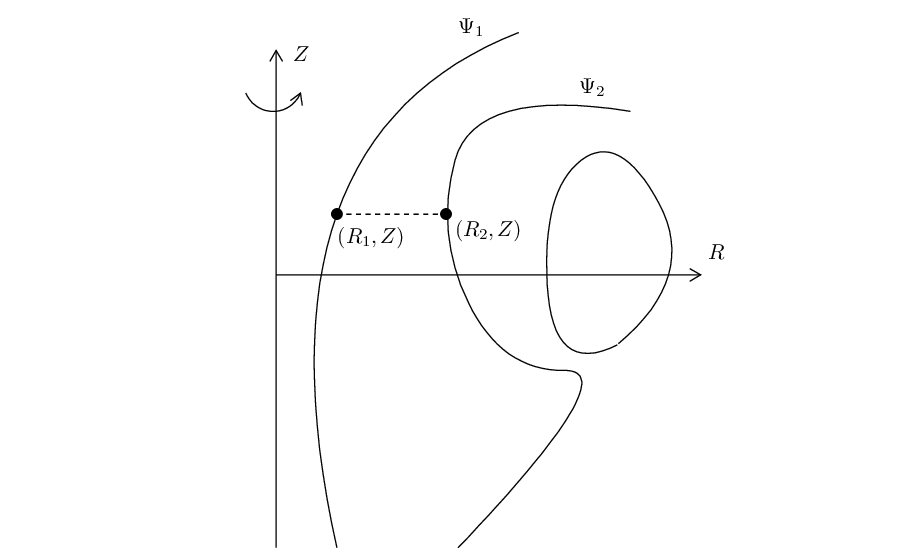
\includegraphics{/home/yj/theory/tokamak_equilibrium/figures/axisymmetrical_magnetic_field-3b.eps}
  \caption{\label{9-8-p1}The poloidal magnetic flux $\Psi_p^{(12)}$ between
  the two magnetic surfaces $\Psi_1$ and $\Psi_2$ is given by $\Psi_p^{(12)} =
  2 \pi (\Psi_2 - \Psi_1)$.}
\end{figure}



In Fig. \ref{9-8-p1}, there are two magnetic surfaces labeled, respectively,
by $\Psi = \Psi_1$ and $\Psi = \Psi_2$. The poloidal magnetic flux through any
toroidal ribbons between the two magnetic surfaces is equal to each other (due
to the magnetic Gauss theorem). Next, we calculate this poloidal magnetic
flux, denoted by $\Psi_p^{(12)}$. To make the calculation easy, we select a
plane perpendicular to the $Z$ axis, as is shown by the dash line in Fig.
(\ref{9-8-p1}). In this case, only $B_Z$ contribute to the poloidal magnetic
flux: (the positive direction of the plane is chosen in the direction of
$\hat{\mathbf{Z}}$)
\begin{eqnarray}
  \Psi_p^{(12)} & = & \int_{R_1}^{R_2} B_z (R, Z) 2 \pi R d R \nonumber\\
  & = & \int_{R_1}^{R_2} \frac{1}{R}  \frac{\partial \Psi}{\partial R} 2 \pi
  R d R \nonumber\\
  & = & 2 \pi \int^{R_2}_{R_1} \frac{\partial \Psi}{\partial R} d R
  \nonumber\\
  & = & 2 \pi [\Psi_2 - \Psi_1] .  \label{7-24-2}
\end{eqnarray}
Equation (\ref{7-24-2}) indicates that the difference of $\Psi$ between two
magnetic surfaces is equal to the poloidal flux divided by $2 \pi$.

In experiments, we measure the poloidal magnetic flux through toroidal loops
around the central symmetric axis (discussed in Sec. \ref{24-11-13-p1}).
Consider one of the loops that located at point $(R, Z)$, then, using
(\ref{7-24-2}), the flux through the loop can be written as
\begin{equation}
  \Psi_p = 2 \pi [\Psi (R, Z) - \Psi (R = 0, Z)],
\end{equation}
The central symmetric axis $(R = 0)$ is a field line. If $A_{\phi}$ is finite
at $R = 0$, then $\Psi = A_{\phi} R$ is zero there. This is the case we
encounter in equilibrium reconstruction. Then this flux is written as
\begin{equation}
  \Psi_p = 2 \pi \Psi (R, Z) .
\end{equation}
Due to this relation, $\Psi$ is often called the poloidal magnetic flux per
radian (SI unit: web/rad). This relation allows the poloidal flux measurements
to be used to constrain the GS equation in the equilibrium reconstrunction
(discussed in Sec. \ref{24-7-5-p1}). Note that the positive normal direction
of the surface (where the magnetic flux $\Psi_p$ is defined) is chosen in the
$+\mathbf{Z}$ direction.

\subsection{Measuring poloidal magnetic flux in
experiments}\label{24-11-13-p1}\label{24-6-26-1}

Tokamaks usually have some toroidal wire loops around the central symmetirc
axis, called flux loops, which are used to measure the poloidal magnetic flux
through the loops. (By measuring the voltage around the loops, we can obtain
the time derivative of the flux and, after integrating over time, the flux
itself.)

Suppose that the loop is located at $(R, Z)$ and denote the magnetic flux
through the loop by $\Psi_p (R, Z, t)$ (only the poloidal magnetic field
contribute to this flux since the loop is in the toroidal direction). Then
Faraday's law gives
\begin{equation}
  \label{8-16-e1} \varepsilon = - \frac{d \Psi_p}{d t},
\end{equation}
where $\varepsilon$ is the emf. If the loop is a coil with $N$ turns, the
induced voltage $V$ in the coil is $N$ times the emf $\varepsilon$, i.e., $V =
N \varepsilon$. Using this, Eq. (\ref{8-16-e1}) is written as
\begin{equation}
  \label{8-16-e2} V = - N \frac{d \Psi_p}{d t} .
\end{equation}
Integrating the above equation over time, we obtain
\begin{equation}
  \label{24-6-25-e1} \Psi_p (R, Z, t) = \Psi_p (R, Z, 0) - \frac{1}{N}
  \int_0^t V dt.
\end{equation}
The starting time $t = 0$ can be chosen as when $\Psi_p (R, Z, 0)$ is easy to
know (e.g., when there is no plasma). Equation (\ref{24-6-25-e1}) tells us how
to calcualte $\Psi_p$ from the measured loop voltage $V$.

There are usually many flux loops (e.g. 35 on EAST{\cite{xiao2007}}) at
different locations in the poloidal plane (see Fig. \ref{19-5-4-p1mm}). They
are outside of the plasma region and thus are \ called ``external magnetic
measurements''. The measured poloidal flux, along with the poloidal field
measurement by magnetic probes, can be used as constraints in reconstructing
the magnetic field within the plasma region. This is discussed in Sec.
\ref{24-7-5-p1}.

\begin{figure}[h]
  \resizebox{0.5\columnwidth}{!}{\includegraphics{/home/yj/theory/heq/fig1b/p.eps}}
  \caption{\label{19-5-4-p1mm}Flux loops (circles) and magnetic probes (blue
  arows) on EAST tokamak. Arrows indicate the positive normal direction of the
  probes.}
\end{figure}

\

\subsection{Closed magnetic surfaces}

In most part of a tokamak plasma, contours of $\Psi$ in $(R, Z)$ plane are
closed before they touch the machine wall. Figure \ref{7-1-p101} shows some
examples of closed flux surfaces.

\begin{figure}[h]
  \resizebox{0.8\columnwidth}{!}{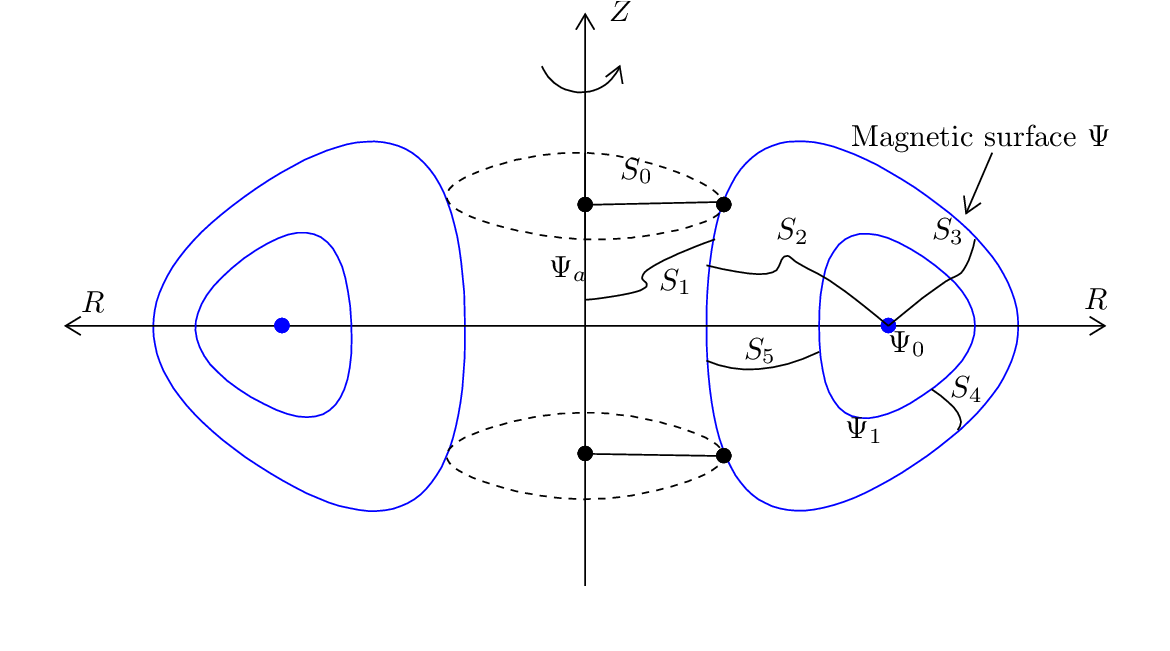
\includegraphics{/home/yj/theory/tokamak_equilibrium/figures/poloidal_flux-1.eps}}
  \caption{\label{7-1-p101}Closed magnetic surfaces (blue) and various
  toroidal surfaces used to define the poloidal magnetic flux. The magnetic
  flux through the toroidal surface $S_2$ and $S_3$ is equal to each other.
  Also the magnetic flux through $S_4$ and $S_5$ is equal to each other; the
  magnetic flux through $S_0$ and $S_1$ is equal to each other.}
\end{figure}

The innermost magnetic surface reduces to a curve, which is called magnetic
axis (in Fig. \ref{7-1-p101}, $\Psi_0$ labels the magnetic axis). $\nabla
\Psi$ is zero at the magnetic axis since $\Psi (R, Z)$ reach maximum/minimum
there. As a result, the poloidal magnetic field is zero there (refer to Eq.
(\ref{20-5-9-p10})).

As is discussed in Sec. \ref{9-5-5}, the poloidal magnetic flux enclosed by a
magnetic surface $\Psi$ (the poloidal magnetic flux through the toroidal
surfaces $S_2$) is given by
\begin{equation}
  \label{12-30-2} \Psi_p^{(\tmop{axis})} = 2 \pi (\Psi_0 - \Psi) .
\end{equation}
Here the positive direction of the surface $S_2$ is defined to be in the
clockwise direction when an observer looks along the direction of
$\hat{\tmmathbf{\phi}}$. In practice, we need to pay attention to the positive
direction chosen (there can be a sign difference when choosing different
positive directions).

Also note, the poloidal magnetic flux enclosed by a closed magnetic surface
can have another definitions: the poloidal magnetic flux through the central
hole of the magnetic surface, i.e., the poloidal flux through $S_1$ in Fig.
\ref{7-1-p101}. In this case, as is discussed in Sec. \ref{9-5-5}, the
poloidal magnetic flux is related to $\Psi$ by
\begin{equation}
  \Psi_p = 2 \pi (\Psi - \Psi (R = 0, Z)) = 2 \pi \Psi,
\end{equation}
where the positive direction of the surface $S_1$ is in the clockwise
direction.

Also note that, since $\mathbf{B}_p = \nabla \Psi \times \nabla \phi$, the
condition $\Psi_{\tmop{LCFS}} - \Psi_{\tmop{axis}} > 0$ means $\mathbf{B}_p$
points in the anticlockwise direction (viewed along $\tmmathbf{\phi}$
direction), and $\Psi_{\tmop{LCFS}} - \Psi_{\tmop{axis}} < 0$ means
$\mathbf{B}_p$ points in the clockwise direction.

\

\section{Non-axisymmetric magnetic perturbations}

In the above, the magnetic field is assumed to be axisymmetric. With this
assumption, the poloidal magnetic field (having two components) can be
expressed in terms of a single component of the vector potential $\mathbf{A}$,
$A_{\phi}$ (specifically via $\Psi \equiv A_{\phi} R$). This kind of
simplification is not achievable if the axisymmetricity assumption is dropped,
because other components of the vector potential (namely $A_R$ and $A_Z$) will
appear in the expression of the poloidal magnetic field. Let us re-examine Eq.
(\ref{4-16-p1}) for a general magnetic perturbation:
\begin{eqnarray}
  \delta \mathbf{B} & = & \left( \frac{1}{R} \frac{\partial \delta
  A_Z}{\partial \phi} - \frac{\partial \delta A_{\phi}}{\partial Z} \right)
  \hat{\mathbf{R}} + \left( \frac{1}{R} \frac{\partial (R \delta
  A_{\phi})}{\partial R} - \frac{1}{R} \frac{\partial \delta A_R}{\partial
  \phi} \right) \hat{\mathbf{Z}} \nonumber\\
  & + & \left( \frac{\partial \delta A_R}{\partial Z} - \frac{\partial \delta
  A_Z}{\partial R} \right) \hat{\tmmathbf{\phi}} .  \label{4-16-p1m}
\end{eqnarray}
When studying tearing modes and turbulence, most authors narrow the possible
perturbations by setting $\delta A_R = \delta A_Z = 0$, i.e.,
\begin{equation}
  \delta B_R = - \frac{1}{R} \frac{\partial \delta \Psi}{\partial Z},
\end{equation}
\begin{equation}
  \delta B_Z = \frac{1}{R} \frac{\partial \delta \Psi}{\partial R},
\end{equation}
\begin{equation}
  \delta B_{\phi} = 0.
\end{equation}
where $\delta \Psi = R \delta A_{\phi}$. Therefore this kind of magnetic
perturbation can still be written in the same form of the equilibrium poloidal
magnetic field:
\begin{equation}
  \delta \mathbf{B}= \nabla \delta \Psi \times \nabla \phi .
\end{equation}
The above approximation is widely used in practice, e.g., in turbulence
simulation, where $\delta A_{\phi}$ is replaced by $\delta A_{\parallel}$. (Do
we miss some magnetic perturbations that is important for plasma transport
when using the above specific form?)

The total magnetic field is then written as
\begin{equation}
  \mathbf{B}= \nabla (\Psi + \delta \Psi) \times \nabla \phi + g \nabla \phi .
\end{equation}
**check**Can the projection of the total magnetic field line in the poloidal
plane can be traced by tracing the contour of $\Psi + \delta \Psi$? No. The
contours of $\Psi + \delta \Psi$ will not show island structures in the
poloidal plane. To show the expected island structures, we need to subtract
non-reconnecting poloidal magnetic field from the total poloidal field?
**check** The contours of the so-called helical flux will give the expected
island structures near the resonant surfaces?**check**

Next, we go back to discuss the 2D case (i.e., assuming axisymmetry).

\section{Plasma current density in terms of $\Psi$ and $g$}

When the displacement current term is neglectable (the case we consider here),
the conductive current is just another representation of the magnetic field.
Specifically, the current density is proportional to the curl of the magnetic
field (Amp{\`e}re's law):
\begin{eqnarray}
  \mu_0 \mathbf{J} & = & \nabla \times \mathbf{B} \nonumber\\
  & = & - \frac{\partial B_{\phi}}{\partial Z} \hat{\mathbf{R}} + \frac{1}{R}
  \frac{\partial (R B_{\phi})}{\partial R} \hat{\mathbf{Z}} + \left(
  \frac{\partial B_R}{\partial Z} - \frac{\partial B_Z}{\partial R} \right)
  \hat{\tmmathbf{\phi}},  \label{3-11-p1}
\end{eqnarray}
where $\mu_0$ is vacuum magnetic permeability.

\subsection{Poloidal current density}

Use Eq. (\ref{3-11-p1}) and the definition $g \equiv R B_{\phi}$, the poloidal
components of the current density, $J_Z$ and $J_R$, can be written as
\begin{equation}
  \label{5-2-a2} \mu_0 J_R = - \frac{1}{R} \frac{\partial g}{\partial Z},
\end{equation}
and
\begin{equation}
  \label{5-2-a1} \mu_0 J_Z = \frac{1}{R} \frac{\partial g}{\partial R},
\end{equation}
respectively.

\subsection{Toroidal current density}

Ampere's law (\ref{3-11-p1}) indicates the toroidal current density $J_{\phi}$
is given by
\begin{eqnarray}
  \mu_0 J_{\phi} & = & \frac{\partial B_R}{\partial Z} - \frac{\partial
  B_Z}{\partial R} \nonumber\\
  & = & - \frac{1}{R} \frac{\partial^2 \Psi}{\partial Z^2} -
  \frac{\partial}{\partial R} \left( \frac{1}{R} \frac{\partial \Psi}{\partial
  R} \right) .  \label{9-5-1}
\end{eqnarray}
Define $\triangle^{\star}$ by
\begin{equation}
  \triangle^{\ast} \equiv \frac{\partial^2}{\partial Z^2} + R
  \frac{\partial}{\partial R} \left( \frac{1}{R} \frac{\partial}{\partial R}
  \right),
\end{equation}
which is the Laplace operator in cylindrical coordinates for the axisymmertic
case, then Eq. (\ref{9-5-1}) is written as
\begin{equation}
  \label{6-9-a1} J_{\phi} = - \frac{1}{\mu_0 R} \triangle^{\ast} \Psi .
\end{equation}
(Many authors refer to Eq. (\ref{6-9-a1}) as the Grad-Shafranov (GS) equation.
No, it is not. It is just Ampere's law, which has nothing to do with the
force-balance. Only after you express $J_{\phi}$ in terms of the plasma
pressure, can Eq. (\ref{6-9-a1}) be called the GS equation, as is discussed
Sec. \ref{24-11-11-2}.)

\section{Constraint of force-balance on magnetic field}\label{24-11-11-1}

Let us consider what constraint the force balance imposes on the axisymmetric
magnetic field discussed above. The MHD momentum equation is given by
\begin{equation}
  \label{19-5-5-1} \rho \left( \frac{\partial \mathbf{u}}{\partial t}
  +\mathbf{u} \cdot \nabla \mathbf{u} \right) = \rho_q \mathbf{E}+\mathbf{J}
  \times \mathbf{B}- \nabla \cdot \mathbb{P}
\end{equation}
where $\rho$, $\rho_q$, $\mathbb{P}$, $\mathbf{J}$, $\mathbf{E}$, and
$\mathbf{B}$ are mass density, charge density, thermal pressure tensor,
current density, electric field, and magnetic field, respectively. The
electric field force $\rho_q \mathbf{E}$ is usually ignored due to either
$\rho_q = 0$ or $\mathbf{E}= 0$. Further assume that there is no plasma flow
($\mathbf{u}= 0$, the flow effect is discussed in \ref{20-4-7-p2}) and the
plasma pressure is isotropic, then the steady state momentum equation (force
balance equation) is written as
\begin{equation}
  \label{7-7-force} \mathbf{J} \times \mathbf{B}= \nabla P,
\end{equation}
where $P$ is the scalar plasma pressure.

Is the force balance (\ref{7-7-force}) always satisfied in a real toakamak
discharge? To answer this question, we need to go back to the original
momentum equation (\ref{19-5-5-1}). The imbalance between $\mathbf{J} \times
\mathbf{B}$ and $\nabla P$ will give rise to the compressional Alfven waves,
the time-scale of which, $\tau_A$, is much shorter than the time-scale $\tau$
we are interested in. Therefore, on the time scale $\tau$ (and for slow flow
with $\mathbf{u}< C_s$, where $C_s$ is the the sound speed), the leading order
of the momentum equation is the force balance
(\ref{7-7-force}).{\cite{ysun2012}}.

\subsection{Parallel force balance }

Consider the force balance in the direction of $\mathbf{B}$. Dotting the
equilibrium equation (\ref{7-7-force}) by $\mathbf{B}$, we obtain
\begin{equation}
  \label{15-11-27-1} 0 =\mathbf{B} \cdot \nabla P,
\end{equation}
which implies that $P$ is constant along a magnetic field line. Since $\Psi$
is also constant along a magnetic field line, $P$ can be expressed in terms of
only $\Psi$ on a single magnetic line. Note that this does not necessarily
mean $P$ is a single-valued function of $\Psi$, (i.e. $P = P (\Psi)$). This is
because $P$ still has the freedom of taking different values on different
magnetic field lines with the same value of $\Psi$ while still satisfying
$\mathbf{B} \cdot \nabla P = 0$. This situation can appear when there are
saddle points (X points) in $\Psi$ contours (refer to Sec. \ref{11-2-p4}) and
$P$ takes different functions of $\Psi$ in islands of $\Psi$ sepearated by a X
point. For pressure within a single island of $\Psi$, $P = P (\Psi)$ can be
safely assumed.

On the other hand, if $P = P (\Psi)$, then we obtain
\[ \mathbf{B} \cdot \nabla P = \frac{d P}{d \Psi} \mathbf{B} \cdot \nabla \Psi
   = 0, \]
i.e., Eq. (\ref{15-11-27-1}) is satisfied, indicating $P = P (\Psi)$ is a
sufficient condition for the force balance in the parallel (to the magnetic
field) direction.

\subsection{Toroidal force balance}

Consider the force balance in the toroidal direction. The $\phi$ component of
Eq. (\ref{7-7-force}) is written
\begin{equation}
  \label{15-11-27-2} J_Z B_R - J_R B_Z = \frac{1}{R} \frac{\partial
  P}{\partial \phi} .
\end{equation}
Since $P = P (\Psi)$, which implies $\partial P / \partial \phi = 0$, equation
(\ref{15-11-27-2}) reduces to
\begin{equation}
  \label{7-7-1} J_Z B_R - J_R B_Z = 0
\end{equation}
Using the expressions of the poloidal current density (\ref{5-2-a2}) and
(\ref{5-2-a1}) in the force balance equation (\ref{7-7-1}) yields
\begin{equation}
  \label{7-8-fai} \frac{\partial g}{\partial R} B_R + \frac{\partial
  g}{\partial Z} B_Z = 0,
\end{equation}
which can be further written
\begin{equation}
  \label{9-7-1} \mathbf{B} \cdot \nabla g = 0.
\end{equation}
According to the same reasoning for the pressure, we conclude that $g = g
(\Psi)$ is a sufficient condition for the toroidal force balance. (The
function $g$ defined here is usually called the ``poloidal current function''
in tokamak literature. The reason for this name is discussed in Sec.
\ref{2-14-10}.)

\subsection{Force balance along the major radius}\label{24-11-11-2}

Consider the force balance in $\hat{\mathbf{R}}$ direction. The
$\hat{\mathbf{R}}$ component of Eq. (\ref{7-7-force}) is written
\begin{equation}
  \label{7-8-radia} J_{\phi} B_Z - J_Z B_{\phi} = \frac{\partial P}{\partial
  R}
\end{equation}
Using the expressions of the current density and magnetic field [Eqs.
(\ref{6-9-a4}) and (\ref{5-2-a1})], equation (\ref{7-8-radia}) is written
\begin{equation}
  \label{3-30-1} J_{\phi} \frac{1}{R} \frac{\partial \Psi}{\partial R} -
  \frac{1}{\mu_0 R} \frac{\partial g}{\partial R}  \frac{g}{R} =
  \frac{\partial P}{\partial R} .
\end{equation}
Assuming the sufficient condition discussed above, i.e., $P$ and $g$ are a
function of only $\Psi$, i.e., $P = P (\Psi)$ and $g = g (\Psi)$, Eq.
(\ref{3-30-1}) is written
\begin{equation}
  J_{\phi} \frac{1}{R} \frac{\partial \Psi}{\partial R} - \frac{1}{\mu_0 R}
  \frac{d g}{d \Psi} \frac{\partial \Psi}{\partial R}  \frac{g}{R} = \frac{d
  P}{d \Psi} \frac{\partial \Psi}{\partial R},
\end{equation}
which can be simplified to
\begin{equation}
  \label{24-5-29-p4} J_{\phi} = R \frac{d P}{d \Psi} + \frac{1}{\mu_0 R}
  \frac{d g}{d \Psi} g,
\end{equation}
which is the requirement of force-balance along the major radius. On the other
hand, we know $J_{\phi}$ can be expressed in $\Psi$ via Eq. (\ref{6-9-a1}).
Combining this with Eq. (\ref{24-5-29-p4}) yields
\begin{equation}
  \triangle^{\ast} \Psi = - \mu_0 R^2 \frac{d P}{d \Psi} - \frac{d g}{d \Psi}
  g,
\end{equation}
i.e.,
\begin{equation}
  \label{7-1-p1} \frac{\partial^2 \Psi}{\partial Z^2} + R
  \frac{\partial}{\partial R} \left( \frac{1}{R} \frac{\partial \Psi}{\partial
  R} \right) = - \mu_0 R^2 \frac{d P}{d \Psi} - \frac{d g}{d \Psi} g.
\end{equation}
Equation (\ref{7-1-p1}) is known as Grad-Shafranov (GS) equation.

[Note that the $Z$ component of the force balance equation is written
\[ \begin{array}{l}
     J_R B_{\phi} - J_{\phi} B_R = \frac{\partial P}{\partial Z}\\
     \Rightarrow - \frac{\partial g}{\partial Z} \frac{1}{R} \frac{g}{R} -
     \frac{1}{R} \triangle^{\ast} \Psi \frac{1}{R} \frac{\partial
     \Psi}{\partial Z} = \mu_0 \frac{d P}{d \Psi} \frac{\partial
     \Psi}{\partial Z}\\
     \Rightarrow - \frac{d g}{d \Psi} \frac{\partial \Psi}{\partial Z}
     \frac{1}{R} \frac{g}{R} - \frac{1}{R} \triangle^{\ast} \Psi \frac{1}{R}
     \frac{\partial \Psi}{\partial Z} = \mu_0 \frac{d P}{d \Psi}
     \frac{\partial \Psi}{\partial Z}\\
     \Rightarrow - \frac{d g}{d \Psi} \frac{1}{R} \frac{g}{R} - \frac{1}{R}
     \triangle^{\ast} \Psi \frac{1}{R} = \mu_0 \frac{d P}{d \Psi}\\
     \Rightarrow \triangle^{\ast} \Psi = - \mu_0 R^2 \frac{d P}{d \Psi} -
     \frac{d g}{d \Psi} g
   \end{array} \]
which turns out to be identical with the Grad-Shafranov equation. This is not
a coincidence. The reason is that the force balance equation has been
satisfied in three different directions (namely, $\hat{\tmmathbf{\phi}}$,
$\hat{\mathbf{R}}$, and $\mathbf{B}$ direction) and thus it must be satisfied
in all the directions.]

\subsection{Axisymmetric equilibrium magnetic field}

A general axisymmetric magnetic field (which does not necessarily satisfy the
force balance), is given by Eq. (\ref{7-28-6}), i.e.,
\begin{equation}
  \label{4-15-p3} \mathbf{B}= \underbrace{\nabla \Psi \times \nabla
  \phi}_{\tmop{poloidal}} + \underbrace{g \nabla \phi}_{\tmop{toroidal}},
\end{equation}
For the above axisymmetric magnetic field to be consistent with the force
balance equation (\ref{7-7-force}), there are additional requirements for
$\Psi$ and $g$. Specifically, $\Psi$ is restricted by the GS equation and $g$
should be a function of only $\Psi$. Therefore an axisymmetric equilibrium
magnetic field is fully determined by two functions, $\Psi = \Psi (R, Z)$ and
$g = g (\Psi)$. The $\Psi$ is determined by solving the GS equation with
specified RHS source terms and boundary conditions.

The RHS source terms in the GS equation (\ref{7-1-p1}) are $P (\Psi)$ and $g
(\Psi)$, both of which must be specified before the GS equation can be solved.
For most cases, the source terms are nonlinear about $\Psi$ and thus the GS
equation is a two-dimensional (in $R$ and $Z$) nonlinear partial differential
equation for $\Psi$.

For most choices of $P (\Psi)$ and $g (\Psi)$, the GS equation (\ref{7-1-p1})
has to be solved numerically. For some particular choices of $P$ and $g$
profiles, analytical solutions are available, one of which is the Solov{\'e}v
equilibrium and is discussed in Appendix \ref{20-4-8-p1}.

Note that we solve the GS equation in order to obtain the poloidal magnetic
flux $\Psi$ and thus the poloidal magnetic field. The toroidal magnetic field
must be specified in some way before we can solve the GS equation. There are
several ways of specifying the toroidal magnetic field: (1) given $g (\Psi)$,
(2) given $\langle j_{\parallel} \rangle$, (3) given the safety factor $q
(\Psi)$. There are simple relations between $g$, $\langle j_{\parallel}
\rangle$, and $q$, which allows translation form one to another (discussed
later). In transport simulations, $\langle j_{\parallel} \rangle$ is obtained
from current drive models and neoclassical bootstrap current models. Note that
the specification of the source terms ($P$, $g$, $q$, and $\langle
j_{\parallel} \rangle$) usually involve the unknown $\Psi$ (via not only the
explicit presence of $\Psi$, but also the flux-surface averaging which
implicit involves $\Psi$). This indicates that iterations are needed when
numerically solving the GS equation.

\subsection{Axisymmetric equilibrium current density}

Since $\mathbf{J}= \mu_0^{- 1} \nabla \times \mathbf{B}$, the current density
$\mathbf{J}$ can be inferred from a given magnetic field. The components of
$\mathbf{J}$ (expressed in terms of $g$ and $\Psi$) are given by Eqs.
(\ref{5-2-a2}), (\ref{5-2-a1}) and (\ref{6-9-a1}) and these expressions can be
further simplified by using the equilibrium constraints, such as $g = g
(\Psi)$ and $\triangle^{\ast} \Psi = - \mu_0 R^2 \frac{d P}{d \Psi} - \frac{d
g}{d \Psi} g$. The simplified $\mathbf{J}$ expressions are given in
\ref{20-4-23-a1}.

On the other hand, in the kinetic equilibrium reconstruction{\cite{li2013}},
it is the current that is first (partially) specified (e.g., by summing
sources of current drive and bootstrap current) and then the current is used
as constraints for the GS equation, i.e, constraints for the magnetic field.

\subsection{Equilibrium scaling}

The GS equation is given by Eq. (\ref{7-1-p1}), i.e.,
\begin{equation}
  \label{23-1-17-p1} \frac{\partial^2 \Psi}{\partial Z^2} + R
  \frac{\partial}{\partial R} \left( \frac{1}{R} \frac{\partial \Psi}{\partial
  R} \right) = - \mu_0 R^2 \frac{d P}{d \Psi} - \frac{d g}{d \Psi} g.
\end{equation}
If a solution to the GS equation is obtained, the solution can be scaled to
obtain a family of solutions. Given an equilibrium with $\Psi (R, Z)$, $P
(\Psi)$, $g (\Psi)$, then it is ready to prove that $\Psi_2 = s \Psi$, $P_2 =
s^2 P (\Psi)$, and $g_2 = \pm s g (\Psi)$ is also a solution to the GS
equation, where $s$ is a constant. In this case, both the poloidal and
toroidal magnetic fields are increased by a factor of $s$, and thus the safety
factor remains unchanged. Also note that the pressure is increased by $s^2$
factor and thus the value of $\beta$ (the ratio of the therm pressure to
magnetic pressure) remains unchanged. Note that $g_2 = \pm s g (\Psi)$, which
indicates that the direction of the toroidal magnetic field can be reversed
without breaking the force balance. Also note that $\Psi_2 = s \Psi$ and $s$
can be negative, which indicates that the direction of the toroidal current
can also be reversed without breaking the force balance.

The second kind of scaling is to set $\Psi_2 = \Psi$, $P_2 = P (\Psi)$, and
$g^2_2 = g^2 (\Psi) + c$. It is ready to prove that the scaled expression is
still a solution to the GS equation because $g_2 g_2' = g g'$. This scaling
keep the pressure and the poloidal field unchanged and thus the poloidal beta
$\beta_p$ remains unchanged. This scaling scales the toroidal field and thus
can be used to generate a family of equilibria with different profiles of
safety factor.

Another scaling, which is trivial, is to set $\Psi_2 = \Psi$, $P_2 = P (\Psi)
+ c$, and $g_2 = g (\Psi)$. This scaling can be used to test the effects of
the pressure (not the pressure gradient) on various physical processes.

When a numerical equilibrium is obtained, one can use these scaling methods
together to generate new equilibria that satisfy particular global conditions.
Note that the shape of magnetic surfaces of the scaled equilibrium remains the
same as the original one.

The above scaling is made under the constraint that the the GS equation
(\ref{23-1-17-p1}), is satisfied. In practice, we may scale $\Psi$ by a factor
while fixing $g$ and $P$. This does not satisfy the GS equation, but allows
more flexibility in changing the the safety factor profile. Scaling $\Psi$ by
a factor corresponds to scaling the plasma current and the poloidal magnetic
field.

\section{Free-boundary fitting problem}\label{24-7-5-p1}

Ampere's law in Eq. (\ref{6-9-a1}) can be generalized to include discrete
toroidal currents:
\begin{eqnarray}
  \triangle^{\ast} \Psi & = & - \mu_0 R J_{\phi} - \mu_0 R \sum_i I_i \delta
  (R - R_i) \delta (Z - Z_i), 
\end{eqnarray}
where $J_{\phi}$ is the plasma toroidal current density, \ $I_i$ is the
toroidal curent in No. $i$ PF coil located at $(R = R_i, Z = Z_i)$, $\delta$
is Dirac's delta function. The solution to the above equation is given by
\begin{equation}
  \label{10-31-1} \Psi (R, Z) = \int_{\Omega} G (R', Z', R, Z) J_{\phi} (R',
  Z') d R' d Z' + \sum_{i = 0}^{N_c - 1} G (R_i, Z_i, R, Z) I_i,
\end{equation}
where $G$ is the fundamental solution given by
\begin{eqnarray}
  &  & G (R', Z', R, Z) \nonumber\\
  & = & \frac{\mu_0 R}{4 \pi} \int_0^{2 \pi} \frac{R' \cos \phi' d
  \phi'}{\sqrt{(Z - Z')^2 + (R - R' \cos \phi')^2 + (R' \sin \phi')^2}}, 
  \label{24-5-29-p2}
\end{eqnarray}
which is often called Green's function in this context. (The Green function is
obtained by using a formula similar to the Biot-Savart Law, see
\ref{24-5-29-p1}.)

If all the toroidal currents (plasma current + PF coil curents) are known,
then $\Psi$ can be calculated by using Eq. (\ref{10-31-1}). Unfortunately
$J_{\phi}$ is usually unknown. On the other hand, the force-balance indicates
that $J_{\phi}$ can be expressed in terms of $\Psi$ via Eq.
(\ref{24-5-29-p4}), i.e.,
\begin{equation}
  \label{24-6-5-5} J_{\phi} = R \frac{d P}{d \Psi} + \frac{1}{\mu_0 R} g
  \frac{d g}{d \Psi} .
\end{equation}
Substituting this into Eq. (\ref{10-31-1}) gives an implicit formula for
$\Psi$, which can be iterated (with an initial guess of $\Psi (R, Z)$, and
assuming the function forms, $P (\Psi)$ and $g (\Psi)$, as well as the coil
currents $I_i$, are known ). Will the iteration converge? We do not know for
sure. Numerical experiments indicate it does in some cases{\cite{lao1985}}.
Let us discuss these cases. We assume that the 1D functions, $P (\Psi)$ and $g
(\Psi)$ can be modeled as (following EFIT's model):
\begin{equation}
  \label{24-6-5-1} \frac{d P (\Psi)}{d \Psi} = \left\{ \begin{array}{l}
    \sum_{j = 0}^{N_P - 1} \alpha_j (x^j - x^{N_p}) \tmop{for} x \leqslant 1\\
    0 \qquad \tmop{for} x > 1
  \end{array} \right.
\end{equation}

\begin{equation}
  \label{24-6-5-2} g \frac{d g}{d \Psi} = \left\{ \begin{array}{l}
    \sum_{j = 0}^{N_F - 1} \beta_j (x^j - x^{N_F}) \tmop{for} x \leqslant 1\\
    0 \qquad \tmop{for} x > 1
  \end{array} \right.
\end{equation}
where
\begin{equation}
  \label{24-11-6-1} x \equiv \overline{\Psi} \equiv \Psi_N \equiv \frac{(\Psi
  - \Psi_M)}{\Psi_B - \Psi_M},
\end{equation}
$\Psi_M$ and $\Psi_B$ are values of $\Psi$ at the magnetic axis and LCFS, the
coefficients $\alpha_j$ and $\beta_j$ are to be determined, $N_p$ and $N_F$
are integers chosen by users. One feature of expressions (\ref{24-6-5-1}) and
(\ref{24-6-5-2}) is that they guarantee that $d P / d \Psi$ and $g d g / d
\Psi$ are zero at and outside the LCFS, and thus no plasma current there. Also
note that expressions (\ref{24-6-5-1}) and (\ref{24-6-5-2}) are nonlinear
functions of $\Psi$ even for $N_p = N_F = 1$. This is because the unknowns,
$\Psi_M$ and $\Psi_B$, appear in the denominator of expression
(\ref{24-11-6-1}). Another nonlinearity is related to the fact that the unkonw
$\Psi$ determines where is the LCFS and thus determine region where the
current desnsity is set to zero. This also gives rise to the name
``free-boundary'' when referring to this kind of problem.

Choosing an initial guess of $\Psi (R, Z)$ on gridpoints, we can get the
values of $\alpha_j$, $\beta_j$, and $I_i$ by solving a least square problem
that minimises the difference between quantities computed and the
corresponding quantities measured in actual experiments. (Details are given in
Sec. \ref{24-11-6-e1}.)

After the coefficients $\alpha_j$ and $\beta_j$ are obtained, $J_{\phi}$ can
be updated by using Eqs. (\ref{24-6-5-5})-(\ref{24-11-6-1}). Then, we use the
latest $J_{\phi}$ and $I_i$ in Eq. (\ref{10-31-1}) to update the values of
$\Psi$ on gridpoints. We repeat the above procedure until convergecne in $\Psi
(R, Z)$. This is called Picard iteration. (Alternatively, the values of $\Psi$
on the inner gridpoints can be updated by inverting the Laplace operator
$\triangle^{\star}$, see Sec. \ref{24-11-14-e1}. The values of $\Psi$ on the
bounary still have to be obtained by using Eq. (\ref{10-31-1}).)

I implemented the above method in a Python code \tmtexttt{HEQ}
(https://github.com/youjunhu/heq). The following subsections discuss details
in the code: Sec. \ref{24-11-8-e3} discusses the least square problem. Sec.
\ref{24-11-8-e1} discusses the vertical displacement instability stabilizer.
Without the stabilizer, the Picard iteration diverges for many elongated
configurations, due to the vertical displacement instability.

\subsection{Response matrix $\Gamma$}\label{24-11-8-e3}\label{24-11-6-e1}

Plugging expressions (\ref{24-6-5-1}) and (\ref{24-6-5-2}) into
(\ref{24-6-5-5}), we obtain
\begin{eqnarray}
  J_{\phi} (R', Z') & = & R' \sum_{j = 0}^{N_p - 1} \alpha_j (x^j - x^{N_p}) +
  \frac{1}{\mu_0 R'} \sum_{j = 0}^{N_F - 1} \beta_j (x^j - x^{N_F}), 
  \label{24-6-5-3}
\end{eqnarray}
For notation ease, define the following basis functions:
\begin{equation}
  b_j (x) = \left\{ \begin{array}{l}
    R' (x^j - x^{N_p}) \hspace{5em} \tmop{for} \quad 0 \leqslant j < N_p\\
    (x^{j - N_p} - x^{N_F}) / (\mu_0 R') \quad \tmop{for} \quad N_p \leqslant
    j < N_p + N_F
  \end{array} \right.
\end{equation}
and the corresponding expansion coefficients
\begin{equation}
  c_j = \left\{ \begin{array}{l}
    \alpha_j \quad \tmop{for} \quad 0 \leqslant j < N_p\\
    \beta_{j - N_p} \quad \tmop{for} \quad N_p \leqslant j < N_p + N_F
  \end{array} \right.
\end{equation}
then Eq. (\ref{24-6-5-3}) is written as
\begin{equation}
  \label{24-6-4-p1} J_{\phi} = \sum_{j = 0}^{N_b - 1} c_j b_j (x),
\end{equation}
where $N_b = N_P + N_F$. Plugging expression (\ref{24-6-4-p1}) into Eq.
(\ref{10-31-1}), we obtain
\begin{eqnarray}
  \Psi (R, Z) & = & \sum_{j = 0}^{N_b - 1} c_j \int_{\Omega} G (R', Z', R, Z)
  b_j (x) d R' d Z' \nonumber\\
  & + & \sum_{j = 0}^{N_c - 1} G (R_j^{(c)}, Z_j^{(c)}, R, Z) I_j . 
  \label{24-6-5-p1}
\end{eqnarray}
Collect all the free parameters as a column vector: $\mathbf{u}= (c_0, \ldots
c_{N_b - 1}, I_0, \ldots, I_{N_c - 1})^T$. Denote the size of vector
$\mathbf{u}$ by $N$, which is the number of free parameters, i.e., $N = N_b +
N_c$, then the rhs of Eq. (\ref{24-6-5-p1}) can be written as matrix-vector
product, $\Gamma \mathbf{u}$. Denote the total number of measurements of the
poloidal flux by $M_{\tmop{FL}}$. Then matrix elements of $\Gamma$ for $i = 0,
\ldots, M_{\tmop{FL}} - 1$ are given by:
\begin{equation}
  \Gamma_{i j} = \int_{\Omega} G (R', Z', R_i^{(\tmop{FL})},
  Z_i^{(\tmop{FL})}) b_j (x) d R' d Z',
\end{equation}
for $j = 0, \ldots, N_b - 1$, and
\begin{equation}
  \Gamma_{i j} = G (R_{j - N_b}^{(c)}, Z_{j - N_b}^{(c)}, R_i^{(\tmop{FL})},
  Z_i^{(\tmop{FL})}),
\end{equation}
for $j = N_b, \ldots, N - 1$. Here $(R_i^{(\tmop{FL})}, Z_i^{(\tmop{FL})})$ is
the location where the $i \tmop{th}$ flux measurement is made.

The matrix $\Gamma$ , which is of shape $(M, N)$, is called ``response
matrix''. (In least square problems, this matrix is called ``design matrix'.)
The value of $M$ is equal to number of measurements included (measurements are
merged to $\Gamma$ by row stacking). We will include $M_{\tmop{FL}}$
measurements of the poloidal flux, $M_B$ measurements of the poloidal magnetic
field, 1 measurement of plasma current, a constraint for the on-axis safety
factor. Then $M = M_{\tmop{FL}} + M_B + 1 + 1$. (For EAST, $M_{\tmop{FL}} =
35, M_B = 38$.)

Next, we consider the poloidal field measurement:
\begin{equation}
  B_p (R_i, Z_i) =\mathbf{B}_p \cdot \hat{\mathbf{n}}_i = B_R \cos \theta_{p
  i} + B_Z \sin \theta_{p i},
\end{equation}
where $(R_i, Z_i)$ is the location of the No. i probe, $\hat{\mathbf{n}}_i$ is
a unit vector denoting the positive normal direction of the No. $i$ magnetic
probe, $\cos \theta_{p i} = \hat{\mathbf{n}}_i \cdot \mathbf{e}_R$, $\sin
\theta_{p i} = \hat{\mathbf{n}}_i \cdot \mathbf{e}_Z$.

$B_p (R_i, Z_i)$ can be inferred from $\mathbf{u}$ via
\begin{eqnarray}
  B_p  (R_i, Z_i) & = & \sum_{j = 0}^{N_b - 1} c_j \int_{\Omega} G_B (R', Z',
  R_i, Z_i) b_j (x) d R' d Z' \nonumber\\
  & + & \sum_{j = 0}^{N_c - 1} G_B (R_j^{(c)}, Z_j^{(c)}, R_i, Z_i) I_j . 
  \label{24-6-6-1}
\end{eqnarray}


where
\begin{equation}
  G_B (R', Z', R_i, Z_i) = G_{B_R} (R', Z', R_i, Z_i) \cos \theta_{p i} +
  G_{B_Z} (R', Z', R_i, Z_i) \sin \theta_{p i},
\end{equation}
and $G_{B_R}$ and $G_{B_Z}$ is given by Eq. (\ref{24-6-6-3}) and
(\ref{24-6-6-4}). The rhs of Eq. (\ref{24-6-6-1}) indicates that the matrix
elements of $\Gamma$ are given by:
\begin{equation}
  \Gamma_{i j} = \int_{\Omega} G_B (R', Z', R_i, Z_i) b_j (x) d R' d Z',
\end{equation}
for  ($j = 0, \ldots, N_b - 1$), and
\begin{equation}
  \Gamma_{i j} = G_B (R_{j - N_b}^{(c)}, Z_{j - N_b}^{(c)}, R_i, Z_i),
\end{equation}
for  ($j = N_b, \ldots, N - 1$) . I place the magnetic field equations after
the flux equations, i.,e the row number $i$ is in the range $[M_{\tmop{FL}},
M_{\tmop{FL}} + M_B - 1]$.

Next, we consider the constraint of plasma current. The plasma current $I_p$
can be inferred from $\mathbf{u}$ via
\begin{equation}
  \label{24-6-6-6} I_p = \int_{\Omega} J_{\phi} d R' d Z' = \sum_{j = 0}^{N_b
  - 1} c_j \int_{\Omega} b_j (x) d R' d Z' .
\end{equation}
The rhs of Eq. (\ref{24-6-6-6}) indicates that the matrix elements of $\Gamma$
are given by:
\begin{equation}
  \Gamma_{i j} = \int_{\Omega} b_j (x) d R' d Z',
\end{equation}
for  ($j = 0, \ldots, N_b - 1$), and zero for  ($j = N_b, \ldots, N - 1$) .
This equation is placed after the equations of flux and magnetic field
measurement, i.e., its row number is \ $i = M_{\tmop{FL}} + M_B$.

Let us consider the constraint of on-axis safety factor value. A formula for
computing $q$ value at the magnetic axis is given by [ref. P. M. Bellan's
paper]:
\begin{equation}
  \label{24-7-17-1} q_{\tmop{axis}} = \frac{e^2 + 1}{e R_{\tmop{axis}}^2}
  \frac{g (0)}{\mu_0 J_{\phi \tmop{axis}}},
\end{equation}
where
\begin{equation}
  e = \sqrt{\left( \frac{\partial^2 \Psi / \partial R^2}{\partial^2 \Psi /
  \partial Z^2} \right)_{\tmop{axis}}},
\end{equation}
is the elongation at the magnetic axis. Using
\[ J_{\phi \tmop{axis}} = \sum_{j = 0}^{N_b - 1} c_j b_j (0) \]
expression (\ref{24-7-17-1}) is written as
\begin{equation}
  \frac{e R_{\tmop{axis}}^2 \mu_0}{(e^2 + 1) g (0)} \sum_{j = 0}^{N_b - 1} c_j
  b_j (0) = \frac{1}{q_{\tmop{axis}}} .
\end{equation}
In \tmtexttt{HEQ}, this constraint is not included in some cases.

\subsection{Algorithm summary}\label{24-11-9-e1}

Step 0. Initial guess of $\Psi$: $\Psi^{(k)}$ with $k = 0$.

Step 1. Compute elements of response matrix $\Gamma$ using $\Psi^{(k)}$.

Step 2. Solve linear least-square problem to get $(c_1, c_2, c_2, c_4, I_1,
\ldots, I_{N_c})$.

Step 3. Update $\Psi$ using the Picard iteration:
\begin{equation}
  \Psi^{(k + 1)} = \int G J_{\phi} (R', \Psi^{(k)}, c_1, c_2, c_3, c_4) d R' d
  Z' + \sum_{n = 1}^{N_c} G I_n,
\end{equation}
\qquad or in its discrete form:
\begin{equation}
  \Psi^{(k + 1)}_{i j} = \sum_{i', j'} G_{i' j' i j} \left( \sum_{n = 1}^4 c_n
  b_{n, i' j'} \right) d S_{i' j'} + \sum_{n = 1}^{N_c} G_{n, i j}^{(c)} I_n .
\end{equation}


Step 4: $k = k + 1$ and goto Step 1.

\

In Step 1, we first search for the magnetic axis and boundary surface of
$\Psi^{(k)}$ so that we can get the values of $\Psi^{(k)}$ at those locations.
These values are needed in computing $x = (\Psi^{(k)} - \Psi_M) / (\Psi_B -
\Psi_M)$.

\subsection{Vertical Displacement Event (VDE) stabilizer in free-boundary
solver{\cite{Jeon2015}}}\label{24-11-8-e1}

\

To stabilize the vertical displacement instability in the Picard iteration,
we add two virtual coils that carry oppositive currents (denoted by
$I_{\tmop{vc}}$ and $- I_{\tmop{vc}}$), and are up-down symmetric, located at
$(R_{\tmop{vc}}, Z_{\tmop{vc}})$ and $(R_{\tmop{vc}}, - Z_{\tmop{vc}})$,
respectively. And set the current $I_{\tmop{vc}}$ by
\[ I_{\tmop{vc}} = - g_z \frac{B_{R, \tmop{vacuum}} (R_{\tmop{cur}},
   Z_{\tmop{cur}})}{G_{B_R} (R_{\tmop{vc}}, Z_{\tmop{vc}}, R_{\tmop{cur}},
   Z_{\tmop{cur}}) - G_{B_R} (R_{\tmop{vc}}, - Z_{\tmop{vc}}, R_{\tmop{cur}},
   Z_{\tmop{cur}})}, \]
where $(R_{\tmop{cur}}, Z_{\tmop{cur}})$ is the location of plasma current
center defined by
\[ R_{\tmop{cur}} = \frac{1}{I_p} \int_{\Omega_{\tmop{pl}}} R J_{\phi} (R, Z)
   d R d Z, \]
\[ Z_{\tmop{cur}} = \frac{1}{I_p} \int_{\Omega_{\tmop{pl}}} Z J_{\phi} (R, Z)
   d R d Z, \]
$B_{R, \tmop{vacuum}}$ is the $B_R$ generated by all the real PF coils, $g_z$
is a positive constant chosen by users. Note that $g = 1$ corresponds to that
the $B_R$ generated by the virtual coils exactly cancles the $B_R$ generted by
all the real coils. Usually we need value larger than 2, i.e., over
compensation. The virtual coils locatons, $(R_{\tmop{vc}}, Z_{\tmop{vc}})$ and
$(R_{\tmop{vc}}, - Z_{\tmop{vc}})$, are usually chosen near the center of the
top/bottom boundary of the computational box.

\subsection{Solving by matrix inversion}\label{24-11-14-e1}

If we want to invert the finite-difference version of the Laplace operator
$\triangle^{\ast}$ to solve the GS equation for $\Psi$, we encounter two
issues: (1) the RHS of the GS equation involves 2 unknown functions $P'
(\Psi)$ and $g g' (\Psi)$, in addition to the main unknown function $\Psi (R,
Z)$; (2) the boundary condition needs to be given: i.e., the values of $\Psi$
on a rectangular computational boundry need to be provided.

To address issue (1): \ function forms of $P' (\Psi)$ and $g' g (\Psi)$ are
chosen by users, often as polymials in $\Psi_N$ with coefficients that are
assumed known (which are later obtained in the least-square method to make the
resulting solution approximately match some measurements, as is discussed in
the previous section).

To address issue (2): The value of $\Psi$ on the rectangular boundary is
updated using the Green's function method (assume that external coil currents
are given), as is discussed in the previous section.

Guess values of $\Psi$ on both the inner gridpoints and boundary points. After
this, we can invert $\triangle^{\ast}$ to update $\Psi$ within the
computational box, and use the Green's function method to update values of
$\Psi$ on the boundary. Then iterate to converge.

Two iterations: one for $\Psi$ values on the inner gridpoints, one over $\Psi$
values on the computational boundary.

External PF coil currents enter the problem via the boundary condition:
specifically via its contribution to $\Psi$ on the boundary.

The above procedure is just a minor modification from the pure Green's
function algorithm discussed in Sec. \ref{24-11-9-e1}, i.e., replacing the
Green's function method for the inner gridpoints with the finte-difference
Laplace operator inverting.

For reference easy, the finite-difference schemes for the Laplace operator is
listed below.
\begin{equation}
  \triangle^{\ast} \Psi = - \mu_0 R J_{\phi}
\end{equation}
\begin{eqnarray}
  \triangle^{\ast} & = & R \frac{\partial}{\partial R} \left( \frac{1}{R}
  \frac{\partial}{\partial R} \right) + \frac{\partial^2}{\partial Z^2} 
  \label{24-7-24-p1}\\
  & = & \frac{\partial}{\partial R^2} - \frac{1}{R} \frac{\partial}{\partial
  R} + \frac{\partial^2}{\partial Z^2}  \label{24-7-24-p2}
\end{eqnarray}


Method 1: discretize Eq. (\ref{24-7-24-p1}) as
\begin{eqnarray}
  &  & R_i \frac{1}{\Delta_R} \left( \left( \frac{1}{R} \frac{\partial
  \Psi}{\partial R} \right)_{i + 1 / 2} - \left( \frac{1}{R} \frac{\partial
  \Psi}{\partial R} \right)_{i - 1 / 2} \right) \nonumber\\
  & + & \frac{\Psi_{i, j + 1} - 2 \Psi_{i, j} + \Psi_{i, j - 1}}{\Delta_Z^2}
  = - \mu_0 R_i J_{\phi i, j}, 
\end{eqnarray}
which can be further discretized as
\begin{eqnarray}
  &  & R_i \frac{1}{\Delta_R} \left( \frac{1}{R_{i + 1 / 2}}  \frac{\Psi_{i +
  1, j} - \Psi_{i, j}}{\Delta_R} - \frac{1}{R_{i - 1 / 2}}  \frac{\Psi_{i, j}
  - \Psi_{i - 1, j}}{\Delta_R} \right) \nonumber\\
  & + & \frac{\Psi_{i, j + 1} - 2 \Psi_{i, j} + \Psi_{i, j - 1}}{\Delta_Z^2}
  = - \mu_0 R_i J_{\phi i, j}, 
\end{eqnarray}
which can be organized as
\[ a \varphi_{i - 1, j} + b \varphi_{i, j} + c \varphi_{i + 1, j} + d
   \varphi_{i, j - 1} + e \varphi_{i, j + 1} = - \mu_0 R_i J_{\phi i, j}, \]
where $b = - \frac{1}{\Delta_R^2}  \left( \frac{R_i}{R_{i + 1 / 2}} +
\frac{R_i}{R_{i - 1 / 2}} \right) - \frac{2}{\Delta_Z^2}$, $a =
\frac{1}{\Delta_R^2} \frac{R_i}{R_{i - 1 / 2}}$, $c = \frac{1}{\Delta_R^2}
\frac{R_i}{R_{i + 1 / 2}}$, $d = e = \frac{1}{\Delta_Z^2}$. Method 2:
discetize Eq. (\ref{24-7-24-p2})
\[ \frac{\Psi_{i + 1, j} - 2 \Psi_{i j} + \Psi_{i - 1, j}}{\Delta_R^2} -
   \frac{1}{R} \frac{\Psi_{i + 1, j} - \Psi_{i - 1, j}}{2 \Delta_R} +
   \frac{\Psi_{i, j + 1} - 2 \Psi_{i, j} + \Psi_{i, j - 1}}{\Delta_Z^2} = -
   \mu_0 R_i J_{\phi i, j}, \]
which can be organized as
\[ a \varphi_{i - 1, j} + b \varphi_{i, j} + c \varphi_{i + 1, j} + d
   \varphi_{i, j - 1} + e \varphi_{i, j + 1} = - \mu_0 R_i J_{\phi i, j}, \]
where $b = - \frac{2}{\Delta_R^2} - \frac{2}{\Delta_Z^2}$ $a =
\frac{1}{\Delta_R^2} + \frac{1}{2 R \Delta_R}$, $c = \frac{1}{\Delta_R^2} -
\frac{1}{2 R \Delta_R}$, $d = e = \frac{1}{\Delta_Z^2}$

My numerical experiments indicate{\tmsamp{}} this scheme is more stable than
than the first one (for the same grid size, and without the VDE stabilizer,
the first scheme blow up while the latter scheme works well).

\section{Semi-free bounday equilibrium problem}

Semi-free boundary equilibrium problems refer to the cases where the LCFS
shape and the value of $\Psi$ on it are given and one is asked to solve the
currents in the PF coils. This is similar to the fitting problem discussed
above: we consider the control points on the LCFS as virtual flux loops that
measure the poloidal flux.

\section{Magnetic control}

An equilibrium reconstruction code (e.g., \tmtexttt{rtefit}) can be used to
``observe'' the inner structure of $\Psi$. PF coil currents can provide
actions on $\Psi$. With the sensors and actuators, we can feedback controll
the magnetic configuration (flux map).

For example, consider controlling the shape of LCFS (often called iso-flux
control). We choose a target surface. To make sure that the target surface is
a magnetic surface, the value of $\Psi$ on it should be made a spatial
constant. Dentoe this constant by $\Psi_t$. To make sure that there is no
closed flux surface outside the target surface, we select the target surface
as a surface that is tangential to the first wall (for limiter configuration)
or there is a X-point on it (for divertor configuration). Then discretize the
target surface by a series of discrete coordinates $(R_i, Z_i)$ with $i = 1,
2, \ldots M$. The actions (coil current changes) are chosen to minimise the
following residual:
\begin{equation}
  \sum_i^M \left( \Delta \Psi_i - \sum_j^{N_c} G (R_j', Z_j', R_i, Z_i) \Delta
  I_j \right)^2,
\end{equation}
where
\begin{equation}
  \Delta \Psi_i = \Psi_t - \Psi_i^{(\tmop{old})},
\end{equation}
\begin{equation}
  \Delta I_j = I_j^{(\tmop{new})} - I_j^{(\tmop{old})},
\end{equation}
the superscritp (old) indicates values before the control actions,
$\Psi_i^{(\tmop{old})}$ is obtained by a real-time equilibrium reconstruction
code.

This assumes that the plasma current density remains the same when the actions
are imposed (i.e., no plasma response is included), so that only the coil
current changes contribute to the $\Psi$ change.

If we need to feedback control $X$ points to derised positions, then the above
sum can be extended to include the following:
\begin{eqnarray}
  &  & \sum_i^{M_X} \left( B_R (R_i^{(X)}, Z_i^{(X)}) + \sum_j^{N_c} G_{B_R}
  (R_j', Z_j', R_i^{(X)}, Z_i^{(X)}) \Delta I_j \right)^2 \nonumber\\
  & + & \sum_i^{M_X} \left( B_Z (R_i^{(X)}, Z_i^{(X)}) + \sum_j^{N_c} G_{B_Z}
  (R_j', Z_j', R_i^{(X)}, Z_i^{(X)}) \Delta I_j \right)^2, 
\end{eqnarray}
where $(R_i^{(X)}, Z_i^{(X)})$ are desired poistions of X points.

\

\

\

\

\section{Fixed boundary equilibrium and choices of coordinates}

Plasma physists love to consider a kind of simplified problem: the fixed
boundary equilibrium problem, where the shape of the boundary flux surface is
given (the value of $\Psi$ is a constant on this boundary). In dealing with
the fixed boundary problem, the curvilinear coordinate system is useful.
Specifically, the convenience is that the coordinates can be adjusted to make
one of the coordinate surfaces coincide with the given boundary flux surface,
so that the boundary condition becomes trivial.

More generally, curvilinear coordinates can be ajusted to make coordinate
surfaces coincide with magnetic surfaces (dicussed later). This often
simplifies analysis of wave and transport problems, especially when we
properly choose the poloidal/toroidal coordinate to make magnetic field lines
look like straight lines in terms of these coordinates.

Next section discusses the basic theory of curvilinear coordinates
system{\cite{boozer2005}}.

In many studies of tokamak plasmas, one need construct a curvilinear
coordinate system based on a given magnetic cofiguration in order to make the
problem amenable to analytical methods or numerical methods. Specifically,
many theories and numerical codes use the curvilinear coordinate systems that
are constructed with one coordinate surface coinciding with magnetic surfaces.
In these coordinate systems, we need to choose a poloidal coordinate $\theta$
and a toroidal coordinate $\zeta$. As metioned above, a particular choice for
$\theta$ and $\zeta$ is one that makes the magnetic field lines be straight
lines in $(\theta, \zeta)$ plane. These kinds of coordinates are often called
magnetic coordinates. That is, ``magnetic coordinates \ are defined so they
conform to the shape of the magnetic surfaces and trivialize the equations for
the field lines.''

A further tuned magnetic coordinate system is the so-called field aligned (or
filed-line following) coordinate system, in which changing one of the three
coordinates with the other two fixed would correspond to following a magnetic
field line. The field aligned coordinates are discussed in Sec.
\ref{21-10-8-1}.

Next, let us discuss some general properties about coordinates transformation.

\subsection{Safety factor}

A magnetic field line on a closed magnetic surface travel a closed curve in a
poloidal plane. For these kinds of field lines, we can define the safety
factor $q$: the number of toroidal loops a magnetic field line travels when it
makes one poloidal loop, i.e.
\begin{equation}
  \label{7-1-p3} q \equiv \frac{\triangle \phi}{2 \pi},
\end{equation}
where $\triangle \phi$ as the change of the toroidal angle when a magnetic
field line travels a full poloidal loop. The safety factor can also be
understood as the average pitch angle of a magnetic field line in $(\theta,
\phi)$ plane of a closed magnetic surface.

For open field line region (where a field line touches the wall before its
poloidal projection can close itself), the ``connection length'' is often used
to characterize the magnetic field.

\subsubsection{Expression of safety factor in terms of magnetic field}

The equation of magnetic field lines is given by
\begin{equation}
  \label{7-1-p2} \frac{R d \phi}{d \ell_p} = \frac{B_{\phi}}{B_p},
\end{equation}
where $d \ell_p$ is the line element along the direction of $\mathbf{B}_p$ on
the poloidal plane. Equation (\ref{7-1-p2}) can be arranged in the form
\begin{equation}
  d \phi = \frac{1}{R} \frac{B_{\phi}}{B_p} d \ell_p,
\end{equation}
which can be integrated over $d \ell_p$ to give
\begin{equation}
  \triangle \phi = \oint \frac{1}{R}  \frac{B_{\phi}}{B_p} d \ell_p,
\end{equation}
where the line integration is along the poloidal magnetic field (the contour
of $\Psi$ on the poloidal plane). Using this, Eq. (\ref{7-1-p3}) is written


\begin{equation}
  \label{9-5-e1} q = \frac{1}{2 \pi} \oint \frac{1}{R}  \frac{B_{\phi}}{B_p} d
  \ell_p .
\end{equation}


\subsubsection{Expression of safety factor in terms of magnetic flux}

The safety factor given by Eq. (\ref{9-5-e1}) is expressed in terms of the
components of the magnetic field. The safety factor can also be expressed in
terms of the magnetic flux. Define $\Delta \Psi_p$ as the poloidal magnetic
flux enclosed by two neighboring magnetic surface, then $\Delta \Psi_p$ is
given by
\begin{equation}
  \label{7-9-dy} \Delta \Psi_p = 2 \pi R \Delta x B_p
\end{equation}
where $\Delta x$ is the length of a line segment in the poloidal plane between
the two magnetic surfaces, which is perpendicular to the first magnetic
surface (so perpendicular to the $\mathbf{B}_p$). Note that $\Delta x$, as
well as $R$ and $B_p$, generally depends on the poloidal location whereas
$\Delta \Psi_p$ is independent of the poloidal location.

Using Eq. (\ref{7-9-dy}), the poloidal magnetic field is written as
\begin{equation}
  \label{7-28} B_p = \frac{1}{2 \pi R}  \frac{\Delta \Psi_p}{\Delta x} .
\end{equation}
Substituting Eq. (\ref{7-28}) into Eq. (\ref{9-5-e1}), we obtain
\begin{equation}
  q = \frac{1}{2 \pi} \oint \frac{1}{R} \frac{B_{\phi}}{B_p} d \ell_p =
  \frac{1}{2 \pi} \oint \frac{1}{R} \frac{2 \pi R \Delta x B_{\phi}}{\Delta
  \Psi_p} d \ell_p = \oint \frac{\Delta x B_{\phi}}{\Delta \Psi_p} d \ell_p .
\end{equation}
We know $\Delta \Psi_p$ is a constant independent of the poloidal location, so
$\Delta \Psi_p$ can be taken outside the integration to give
\begin{equation}
  \label{17-11-12-1} q = \frac{1}{\Delta \Psi_p} \oint \Delta x B_{\phi} d
  \ell_p
\end{equation}
It is ready to realise that the integral appearing in Eq. (\ref{17-11-12-1})
is the toroidal magnetic flux enclosed by the two magnetic surfaces, $\Delta
\Psi_t$. Using this, Eq. (\ref{17-11-12-1}) is written as
\begin{equation}
  \label{9-6-p2} q = \frac{\Delta \Psi_t}{\Delta \Psi_p}
\end{equation}
Equation (\ref{9-6-p2}) indicates that the safety factor of a magnetic surface
is equal to the differential of the toroidal magnetic flux with respect to the
poloidal magnetic flux enclosed by the magnetic surface.

\

\subsubsection{Rational surfaces vs. irrational surfaces}

If the safety factor of a magnetic surface is a rational number, i.e., $q = m
/ n$, where $m$ and $n$ are integers, then this magnetic surface is called a
rational surface, otherwise an irrational surface. A field line on a rational
surface with $q = m / n$ closes itself after it travels $n$ poloidal loops. An
example of a field line on a rational surface is shown in Fig. \ref{17-1-1-1}.

\begin{figure}[h]
  \resizebox{0.5\columnwidth}{!}{\includegraphics{/home/yj/project_new/nbi_fig/fig12/p.eps}}\resizebox{0.5\columnwidth}{!}{\includegraphics{/home/yj/project_new/nbi_fig/fig12b/p.eps}}
  \caption{\label{17-1-1-1}Left: A magnetic field line (blue) on a rational
  surface with $q = 2.1 = 21 / 10$ (magnetic field is from EAST discharge
  \#59954@3.1s). This field line closes itself after traveling 21 toroidal
  loops (meanwhile, it travels 10 poloidal loops). Right: The intersecting
  points of the magnetic field line with the $\phi = 0$ plane when it is
  traveling toroidally. The sequence of the intersecting points is indicated
  by the number labels. The 22nd intersecting point coincides with the 1st
  point and then the intersecting points repeat themselves.}
\end{figure}

\

\section{Curvilinear coordinate system}

\subsection{Coordinates transformation}

In the Cartesian coordinates, a point is described by its coordinates $(x, y,
z)$, which, in the vector form, is written as
\begin{equation}
  \mathbf{r}= x \hat{\mathbf{x}} + y \hat{\mathbf{y}} + z \hat{\mathbf{z}},
\end{equation}
where $\mathbf{r}$ is the location vector of the point; $\hat{\mathbf{x}}$,
$\hat{\mathbf{y}}$, and $\hat{\mathbf{z}}$ are the basis vectors of the
Cartesian coordinates, which are constant, independent of spactial location.
The transformation between the Cartesian coordinates system, $(x, y, z)$, and
a general coordinates system, $(x_1, x_2, x_3)$, can be expressed as
\begin{equation}
  \label{11-8-10dd} \mathbf{r}= x (x_1, x_2, x_3) \hat{\mathbf{x}} + y (x_1,
  x_2, x_3) \hat{\mathbf{y}} + z (x_1, x_2, x_3) \hat{\mathbf{z}} .
\end{equation}
For example, cylindrical coordinates $(R, \phi, Z)$ can be considered as a
general coordinate systems, which are defined by \ $\mathbf{r}= R \cos \phi
\hat{\mathbf{x}} + R \sin \phi \hat{\mathbf{y}} + Z \hat{\mathbf{z}}$.

The transformation function in Eq. (\ref{11-8-10dd}) can be written as
\begin{equation}
  \label{11-8-10} \begin{array}{l}
    x = x (x_1, x_2, x_3)\\
    y = y (x_1, x_2, x_3)\\
    z = z (x_1, x_2, x_3)
  \end{array}
\end{equation}

\subsection{Jacobian}

A useful quality characterizing coordinate transformation is the Jacobian
determinant (or simply called Jacobian), which, for the transformation in Eq.
(\ref{11-8-10}), is defined by
\begin{equation}
  \label{21-11-29-1} \mathcal{J}= \left|\begin{array}{ccc}
    \frac{\partial x}{\partial x_1} & \frac{\partial x}{\partial x_2} &
    \frac{\partial x}{\partial x_3}\\
    \frac{\partial y}{\partial x_1} & \frac{\partial y}{\partial x_2} &
    \frac{\partial y}{\partial x_3}\\
    \frac{\partial z}{\partial x_1} & \frac{\partial z}{\partial x_2} &
    \frac{\partial z}{\partial x_3}
  \end{array}\right|,
\end{equation}
which can also be written as
\begin{equation}
  \label{10-21-p3} \mathcal{J}= \frac{\partial \mathbf{r}}{\partial x_1}
  \times \frac{\partial \mathbf{r}}{\partial x_2} \cdot \frac{\partial
  \mathbf{r}}{\partial x_3} .
\end{equation}
It is easy to prove that the Jacobian $\mathcal{J}$ in Eq. (\ref{10-21-p3})
can also be written (the derivation is given in my notes on Jacobian)
\begin{equation}
  \label{10-21-p4} \mathcal{J}= (\nabla x_1 \times \nabla x_2 \cdot \nabla
  x_3)^{- 1} .
\end{equation}
Conventionally, the Jacobian of the transformation from the Cartesian
coordinates to a particular coordinate system $\sigma$ is called the Jacobian
of $\sigma$, without explitly mentioning that this transformation is with
respect to the Cartesian coordinates.

Using the defintion in Eq. (\ref{21-11-29-1}), the Jacobian $\mathcal{J}$ of
the Cartesian coordinates can be calculated, yielding $1$. Likewise, the
Jacobian of the cylindrical coordinates $(R, \phi, Z)$ can be calculated as
follows:
\begin{eqnarray*}
  \mathcal{J} & = & \left|\begin{array}{ccc}
    \frac{\partial x}{\partial R} & \frac{\partial x}{\partial \phi} &
    \frac{\partial x}{\partial Z}\\
    \frac{\partial y}{\partial R} & \frac{\partial y}{\partial \phi} &
    \frac{\partial y}{\partial Z}\\
    \frac{\partial z}{\partial R} & \frac{\partial z}{\partial \phi} &
    \frac{\partial z}{\partial Z}
  \end{array}\right| = \left|\begin{array}{ccc}
    \frac{\partial R \cos \phi}{\partial R} & \frac{\partial R \cos
    \phi}{\partial \phi} & \frac{\partial R \cos \phi}{\partial Z}\\
    \frac{\partial R \sin \phi}{\partial R} & \frac{\partial R \sin
    \phi}{\partial \phi} & \frac{\partial R \sin \phi}{\partial Z}\\
    \frac{\partial Z}{\partial R} & \frac{\partial Z}{\partial \phi} &
    \frac{\partial Z}{\partial Z}
  \end{array}\right|\\
  & = & \left|\begin{array}{ccc}
    \cos \phi & - R \sin \phi & 0\\
    \sin \phi & R \cos \phi & 0\\
    0 & 0 & 1
  \end{array}\right| = R
\end{eqnarray*}
If the Jacobian of a coordinate system is greater than zero, it is called a
right-handed coordinate system. Otherwise it is called a left-handed system.

\subsection{Orthogonality relation between two sets of basis vectors}

In a curvilinear coordinate system $(x_1, x_2, x_3)$, there are two kinds of
basis vectors: $\nabla x_i$ and $\partial \mathbf{r}/ \partial x_i$, with $i =
1, 2, 3.$ These two kinds of basis vectors satisfy the following orthogonality
relation:
\begin{equation}
  \label{4-6-e1} \nabla x_i \cdot \frac{\partial \mathbf{r}}{\partial x_j} =
  \delta_{i j},
\end{equation}
where $\delta_{i j}$ is the Kronical delta function. [Proof: Working in a
Cartesian coordinate system $(x, y, z)$ with the corresponding basis vectors
denoted by $(\hat{\mathbf{x}}, \hat{\mathbf{y}}, \hat{\mathbf{z}})$, then the
left-hand side of Eq. (\ref{4-6-e1}) can be written as
\begin{eqnarray}
  \nabla x_i \cdot \frac{\partial \mathbf{r}}{\partial x_j} & = & \left[
  \left( \frac{\partial x_i}{\partial x} \right) \hat{\mathbf{x}} + \left(
  \frac{\partial x_i}{\partial y} \right) \hat{\mathbf{y}} + \left(
  \frac{\partial x_i}{\partial z} \right) \hat{\mathbf{z}} \right] \cdot
  \left[ \frac{\partial x}{\partial x_j} \hat{\mathbf{x}} + x \frac{\partial
  \hat{\mathbf{x}}}{\partial x_j} + \frac{\partial y}{\partial x_j}
  \hat{\mathbf{y}} + y \frac{\partial \hat{\mathbf{y}}}{\partial x_j} +
  \frac{\partial z}{\partial x_j} \hat{\mathbf{z}} + z \frac{\partial
  \hat{\mathbf{z}}}{\partial x_j} \right] \nonumber\\
  & = & \left[ \left( \frac{\partial x_i}{\partial x} \right)
  \hat{\mathbf{x}} + \left( \frac{\partial x_i}{\partial y} \right)
  \hat{\mathbf{y}} + \left( \frac{\partial x_i}{\partial z} \right)
  \hat{\mathbf{z}} \right] \cdot \left[ \frac{\partial x}{\partial x_j}
  \hat{\mathbf{x}} + 0 + \frac{\partial y}{\partial x_j} \hat{\mathbf{y}} + 0
  + \frac{\partial z}{\partial x_j} \hat{\mathbf{z}} + 0 \right] \\
  & = & \frac{\partial x_i}{\partial x} \frac{\partial x}{\partial x_j} +
  \frac{\partial x_i}{\partial y}  \frac{\partial y}{\partial x_j} +
  \frac{\partial x_i}{\partial z}  \frac{\partial z}{\partial x_j} \nonumber\\
  & = & \frac{\partial x_i}{\partial x_j}  \label{18-10-10-p1}\\
  & = & \delta_{i j}, \nonumber
\end{eqnarray}
where the second equality is due to $\partial \hat{\mathbf{x}} / \partial x^j
= 0, \partial \hat{\mathbf{y}} / \partial x^j = 0, \partial \hat{\mathbf{z}} /
\partial x^j = 0$ since $\hat{\mathbf{x}}, \hat{\mathbf{y}}, \hat{\mathbf{z}}$
are constant vectors independent of spatial location; the chain rule has been
used in obtaining Eq. (\ref{18-10-10-p1})]

[The cylindrical coordinate system $(R, \phi, Z)$ is an example of general
coordinates. As an exercise, we can verify that the cylindrical coordinates
have the property given in Eq. (\ref{4-6-e1}). In this case, $x = x_1 \cos
x_2$, $y = x_1 \sin x_2$, $z = x_3$, where $x_1 \equiv R$, $x_2 \equiv \phi$,
$x_3 \equiv Z$.]

It can be proved that $\nabla x^i$ is a contravariant vector while $\partial
\mathbf{r}/ \partial x^i$ is a covariant vector (I do not prove this and do
not bother with the meaning of these names, just using this as a naming scheme
for easy reference).

The orthogonality relation in Eq. (\ref{4-6-e1}) is fundamental to the theory
of general coordinates. The orthogonality relation allows one to write the
covariant basis vectors in terms of contravariant basis vectors and vice
versa. For example, the orthogonality relation tells that $\partial
\mathbf{r}/ \partial x_1$ is orthogonal to $\nabla x_2$ and $\nabla x_3$,
thus, $\partial \mathbf{r}/ \partial x_1$ can be written as
\begin{equation}
  \label{9-7-4} \frac{\partial \mathbf{r}}{\partial x_1} = A \nabla x_2 \times
  \nabla x_3,
\end{equation}
where $A$ is a unknown variable to be determined. To determine $A$, dotting
Eq. (\ref{9-7-4}) by $\nabla x_1$, and using the orthogonality relation again,
we obtain
\begin{equation}
  1 = A (\nabla x_2 \times \nabla x_3) \cdot \nabla x_1,
\end{equation}
which gives
\begin{eqnarray}
  A & = & \frac{1}{(\nabla x_2 \times \nabla x_3) \cdot \nabla x_1}
  \nonumber\\
  & = & \mathcal{J} 
\end{eqnarray}
Thus $\partial \mathbf{r}/ \partial x_1$ is written, in terms of $\nabla x_1$,
$\nabla x_2$, and $\nabla x_3$, as
\begin{equation}
  \label{9-8-1} \frac{\partial \mathbf{r}}{\partial x_1} =\mathcal{J} \nabla
  x_2 \times \nabla x_3 .
\end{equation}
Similarly, we obtain
\begin{equation}
  \label{9-8-2} \frac{\partial \mathbf{r}}{\partial x_2} =\mathcal{J} \nabla
  x_3 \times \nabla x_1
\end{equation}
and
\begin{equation}
  \label{9-8-3} \frac{\partial \mathbf{r}}{\partial x_3} =\mathcal{J} \nabla
  x_1 \times \nabla x_2 .
\end{equation}
Equations (\ref{9-8-1})-(\ref{9-8-3}) can be generally written
\begin{equation}
  \label{11-18-1} \frac{\partial \mathbf{r}}{\partial x_i} =\mathcal{J} \nabla
  x_j \times \nabla x_k,
\end{equation}
where $(i, j, k)$ represents the cyclic order in the variables $(x_1, x_2,
x_3)$. Equation (\ref{11-18-1}) expresses the covariant basis vectors in terms
of the contravariant basis vectors. On the other hand, from Eq.
(\ref{9-8-1})-(\ref{9-8-3}), we obtain
\begin{equation}
  \label{20-10-15-a1} \nabla x_i =\mathcal{J}^{- 1} \frac{\partial
  \mathbf{r}}{\partial x_j} \times \frac{\partial \mathbf{r}}{\partial x_k},
\end{equation}
which expresses the contravariant basis vectors in terms of the covariant
basis vectors.

\subsection{An example: ($\psi, \theta, \zeta$) coordinates}

Suppose $(\psi, \theta, \zeta)$ is an arbitrary general coordinate system.
Following Einstein's notation, contravariant basis vectors are denoted with
upper indices as
\begin{eqnarray}
  \mathbf{e}^{\psi} \equiv \nabla \psi ; & \mathbf{e}^{\theta} \equiv \nabla
  \theta ; & \mathbf{e}^{\zeta} \equiv \nabla \zeta . 
\end{eqnarray}
and the covariant basis vectors are denoted with low indices as
\begin{eqnarray}
  \mathbf{e}_{\psi} \equiv \frac{\partial \mathbf{r}}{\partial \psi} ; &
  \mathbf{e}_{\theta} \equiv \frac{\partial \mathbf{r}}{\partial \theta} ; &
  \mathbf{e}_{\zeta} \equiv \frac{\partial \mathbf{r}}{\partial \zeta} . 
\end{eqnarray}
Then the orthogonality relation, Eq. (\ref{4-6-e1}), is written as
\begin{equation}
  \mathbf{e}^{\alpha} \cdot \mathbf{e}_{\beta} = \delta_{\alpha \beta} .
\end{equation}
In term of the contravairant basis vectors, $\mathbf{A}$ is written
\begin{equation}
  \label{9-8-8} \mathbf{A}= A_{\psi} \mathbf{e}^{\psi} + A_{\theta}
  \mathbf{e}^{\theta} + A_{\zeta} \mathbf{e}^{\zeta},
\end{equation}
where the components are easily obtained by taking scalar product with
$\mathbf{e}_{\psi}, \mathbf{e}_{\theta}, \tmop{and} \mathbf{e}_{\zeta}$,
yielding $A_{\psi} =\mathbf{A} \cdot \mathbf{e}_{\psi}$, $A_{\theta}
=\mathbf{A} \cdot \mathbf{e}_{\theta}$, and $A_{\zeta} =\mathbf{A} \cdot
\mathbf{e}_{\zeta}$. Similarly, in term of the covariant basis vectors,
$\mathbf{A}$ is written
\begin{equation}
  \label{9-8-7} \mathbf{A}= A^{\psi} \mathbf{e}_{\psi} + A^{\theta}
  \mathbf{e}_{\theta} + A^{\zeta} \mathbf{e}_{\zeta},
\end{equation}
where $A^{\psi} =\mathbf{A} \cdot \mathbf{e}^{\psi}$, $A^{\theta} =\mathbf{A}
\cdot \mathbf{e}^{\theta}$, and $A^{\zeta} =\mathbf{A} \cdot
\mathbf{e}^{\zeta}$.

Using the above notation, the relation in Eq. (\ref{11-18-1}) is written as
\begin{equation}
  \mathbf{e}_{\psi} = \mathcal{J} \mathbf{e}^{\theta} \times
  \mathbf{e}^{\zeta}
\end{equation}
\begin{equation}
  \mathbf{e}_{\theta} = \mathcal{J} \mathbf{e}^{\zeta} \times
  \mathbf{e}^{\psi}
\end{equation}
\begin{equation}
  \mathbf{e}_{\zeta} = \mathcal{J} \mathbf{e}^{\psi} \times
  \mathbf{e}^{\theta}
\end{equation}
where \ $\mathcal{J} = [(\nabla \psi \times \nabla \theta) \cdot \nabla
\zeta]^{- 1}$. Similarly, the relation in Eq. (\ref{20-10-15-a1}) is written
as
\begin{equation}
  \mathbf{e}^{\psi} = \mathcal{J}^{- 1} \mathbf{e}_{\theta} \times
  \mathbf{e}_{\zeta}
\end{equation}
\begin{equation}
  \mathbf{e}^{\theta} = \mathcal{J}^{- 1} \mathbf{e}_{\zeta} \times
  \mathbf{e}_{\psi}
\end{equation}
\begin{equation}
  \mathbf{e}^{\zeta} = \mathcal{J}^{- 1} \mathbf{e}_{\psi} \times
  \mathbf{e}_{\theta}
\end{equation}

\subsection{Gradient and directional derivative in general coordinates $(\psi,
\theta, \zeta)$}

The gradient of a scalar function $f (\psi, \theta, \zeta)$ is readily
calculated from the chain rule,
\begin{equation}
  \label{5-6-5} \nabla f = \frac{\partial f}{\partial \psi} \nabla \psi +
  \frac{\partial f}{\partial \theta} \nabla \theta + \frac{\partial
  f}{\partial \zeta} \nabla \zeta .
\end{equation}
Note that the gradient of a scalar function is in the covariant
representation. The inverse form of this expression is obtained by dotting the
above equation respectively by the three contravariant basis vectors, yielding
\begin{equation}
  \label{4-6-1} \frac{\partial f}{\partial \psi} = (\mathcal{J} \nabla \theta
  \times \nabla \zeta) \cdot \nabla f = \frac{\partial \mathbf{r}}{\partial
  \psi} \cdot \nabla f
\end{equation}
\begin{equation}
  \label{4-6-2} \frac{\partial f}{\partial \theta} = (\mathcal{J} \nabla \zeta
  \times \nabla \psi) \cdot \nabla f = \frac{\partial \mathbf{r}}{\partial
  \theta} \cdot \nabla f
\end{equation}
\begin{equation}
  \label{4-6-3} \frac{\partial f}{\partial \zeta} = (\mathcal{J} \nabla \psi
  \times \nabla \theta) \cdot \nabla f = \frac{\partial \mathbf{r}}{\partial
  \zeta} \cdot \nabla f
\end{equation}
Using Eq. (\ref{5-6-5}), the directional derivative in the direction of
$\nabla \psi$ is written as
\begin{equation}
  \nabla \psi \cdot \nabla f = | \nabla \psi |^2 \frac{\partial f}{\partial
  \psi} + (\nabla \theta \cdot \nabla \psi) \frac{\partial f}{\partial \theta}
  + (\nabla \zeta \cdot \nabla \psi) \frac{\partial f}{\partial \zeta} .
\end{equation}

\subsection{Divergence operator in general coordinates $(\psi, \theta,
\zeta)$}

To calculate the divergence of a vector, it is desired that the vector should
be in the contravariant form because we can make use of the fact:
\begin{equation}
  \nabla \cdot (\nabla \alpha \times \nabla \beta) = 0,
\end{equation}
for any scalar quantities $\alpha$ and $\beta$. Therefore we write vector
$\mathbf{A}$ as
\begin{equation}
  \mathbf{A}= A^{(\psi)} \mathcal{J} \nabla \theta \times \nabla \zeta +
  A^{(\theta)} \mathcal{J} \nabla \zeta \times \nabla \psi + A^{(\zeta)}
  \mathcal{J} \nabla \psi \times \nabla \theta,
\end{equation}
where $A^{(\psi)} =\mathbf{A} \cdot \nabla \psi$, $A^{(\theta)} =\mathbf{A}
\cdot \nabla \theta$, $A^{(\zeta)} =\mathbf{A} \cdot \nabla \zeta$. \ \ Then
the divergence of $\mathbf{A}$ is readily calculated as
\begin{eqnarray}
  \nabla \cdot \mathbf{A} & = & (\nabla \theta \times \nabla \zeta) \cdot
  \nabla (A^{(\psi)} \mathcal{J}) + (\nabla \zeta \times \nabla \psi) \cdot
  \nabla (A^{(\theta)} \mathcal{J}) + (\nabla \psi \times \nabla \theta) \cdot
  \nabla (A^{(\zeta)} \mathcal{J}) \\
  & = & \frac{1}{\mathcal{J}} \left( \frac{\partial A^{(\psi)}
  \mathcal{J}}{\partial \psi} + \frac{\partial A^{(\theta)}
  \mathcal{J}}{\partial \theta} + \frac{\partial A^{(\zeta)}
  \mathcal{J}}{\partial \zeta} \right),  \label{6-8-e5}
\end{eqnarray}
where the second equality is obtained by using Eqs. (\ref{4-6-1}),
(\ref{4-6-2}), and (\ref{4-6-3}).

\subsection{Laplacian operator in general coordinates $(\psi, \theta, \zeta)$}

The Laplacian operator is defined by $\nabla^2 \equiv \nabla \cdot \nabla$.
Then $\nabla^2 f$ is written as ($f$ is an arbitrary function)
\begin{eqnarray}
  \nabla^2 f & = & \nabla \cdot \nabla f \nonumber\\
  & = & \nabla \cdot \left( \tmcolor{blue}{\frac{\partial f}{\partial \psi}
  \nabla \psi + \frac{\partial f}{\partial \theta} \nabla \theta +
  \frac{\partial f}{\partial \zeta} \nabla \zeta} \right) .  \label{19-1-15-1}
\end{eqnarray}
To proceed, we can use the divergence formula (\ref{6-8-e5}) to express the
divergence in the above expression. However, the vector in the above
(\tmcolor{blue}{blue term}) is not in the covariant form desired by the
divergence formula (\ref{6-8-e5}). If we want to directly use the formula
(\ref{6-8-e5}), we need to transform the vector (\tmcolor{blue}{blue term} in
expression (\ref{19-1-15-1})) to the covariant form. This process seems to be
a little complicated. Therefore, I choose not to use this method. Instead, I
try to simplify expression (\ref{19-1-15-1}) by using basic vector identities:
\begin{eqnarray}
  \nabla^2 f & = & \nabla \left( \frac{\partial f}{\partial \psi} \right)
  \cdot \nabla \psi + \nabla \left( \frac{\partial f}{\partial \theta} \right)
  \cdot \nabla \theta + \nabla \left( \frac{\partial f}{\partial \zeta}
  \right) \cdot \nabla \zeta \nonumber\\
  &  & + \frac{\partial f}{\partial \psi} \nabla^2 \psi + \frac{\partial
  f}{\partial \theta} \nabla^2 \theta + \frac{\partial f}{\partial \zeta}
  \nabla^2 \zeta . 
\end{eqnarray}
Using the gradient formula, the above expression is further written as
\begin{eqnarray}
  \nabla^2 f & = & \frac{\partial^2 f}{\partial \psi^2} | \nabla \psi |^2 +
  \frac{\partial^2 f}{\partial \psi \partial \theta} \nabla \psi \cdot \nabla
  \theta + \frac{\partial^2 f}{\partial \psi \partial \zeta} \nabla \psi \cdot
  \nabla \zeta \nonumber\\
  &  & + \frac{\partial^2 f}{\partial \theta \partial \psi} \nabla \theta
  \cdot \nabla \psi + \frac{\partial^2 f}{\partial \theta^2} | \nabla \theta
  |^2 + \frac{\partial^2 f}{\partial \theta \partial \zeta} \nabla \theta
  \cdot \nabla \zeta \nonumber\\
  &  & + \frac{\partial^2 f}{\partial \zeta \partial \psi} \nabla \zeta \cdot
  \nabla \psi + \frac{\partial^2 f}{\partial \zeta \partial \theta} \nabla
  \zeta \cdot \nabla \theta + \frac{\partial^2 f}{\partial \zeta^2} | \nabla
  \zeta |^2 \nonumber\\
  &  & + \frac{\partial f}{\partial \psi} \nabla^2 \psi + \frac{\partial
  f}{\partial \theta} \nabla^2 \theta + \frac{\partial f}{\partial \zeta}
  \nabla^2 \zeta, 
\end{eqnarray}
and can be simplified as
\begin{eqnarray}
  \nabla^2 f & = & \frac{\partial^2 f}{\partial \psi^2} | \nabla \psi |^2 + 2
  \frac{\partial^2 f}{\partial \psi \partial \theta} \nabla \psi \cdot \nabla
  \theta + 2 \frac{\partial^2 f}{\partial \psi \partial \zeta} \nabla \psi
  \cdot \nabla \zeta \nonumber\\
  &  & + \frac{\partial^2 f}{\partial \theta^2} | \nabla \theta |^2 + 2
  \frac{\partial^2 f}{\partial \theta \partial \zeta} \nabla \theta \cdot
  \nabla \zeta \nonumber\\
  &  & + \frac{\partial^2 f}{\partial \zeta^2} | \nabla \zeta |^2 \nonumber\\
  &  & + \frac{\partial f}{\partial \psi} \nabla^2 \psi + \frac{\partial
  f}{\partial \theta} \nabla^2 \theta + \frac{\partial f}{\partial \zeta}
  \nabla^2 \zeta . 
\end{eqnarray}
Assume $(\psi, \theta, \zeta)$ are field-line following coordinates with
$\partial \mathbf{r}/ \partial \theta$ along the field line direction, then
neglect all the parallel derivatives, i.e., derivative over $\theta$, then the
above expression is reduced to
\begin{eqnarray}
  \nabla^2 f & = & \frac{\partial^2 f}{\partial \psi^2} | \nabla \psi |^2 + 2
  \frac{\partial^2 f}{\partial \psi \partial \zeta} \nabla \psi \cdot \nabla
  \zeta + \frac{\partial^2 f}{\partial \zeta^2} | \nabla \zeta |^2 \nonumber\\
  &  & + \frac{\partial f}{\partial \psi} \nabla^2 \psi + \frac{\partial
  f}{\partial \zeta} \nabla^2 \zeta . 
\end{eqnarray}
This approximation reduces the Laplacian operator from being three-dimensional
to being two-dimensional. This approximation is often called the high-$n$
approximation, where $n$ is the toroidal mode number (mode number along
$\zeta$ direction).

\subsection{Curl operator in general coordinates $(\psi, \theta, \zeta)$}

To take the curl of a vector, it should be in the covariant representation
since we can make use of the fact that $\nabla \times \nabla \alpha = 0$. Thus
the curl of $\mathbf{A}$ is written as
\begin{eqnarray}
  \nabla \times \mathbf{A} & = & \nabla \times (A_1 \nabla \psi + A_2 \nabla
  \theta + A_3 \nabla \zeta) \nonumber\\
  & = & \nabla A_1 \times \nabla \psi + \nabla A_2 \times \nabla \theta +
  \nabla A_3 \times \nabla \zeta \nonumber\\
  & = & \left( \frac{\partial A_1}{\partial \theta} \nabla \theta +
  \frac{\partial A_1}{\partial \zeta} \nabla \zeta \right) \times \nabla \psi
  + \left( \frac{\partial A_2}{\partial \psi} \nabla \psi + \frac{\partial
  A_2}{\partial \zeta} \nabla \zeta \right) \times \nabla \theta + \left(
  \frac{\partial A_3}{\partial \psi} \nabla \psi + \frac{\partial
  A_3}{\partial \theta} \nabla \theta \right) \times \nabla \zeta \nonumber\\
  & = & \frac{1}{\mathcal{J}} \left( \frac{\partial A_2}{\partial \psi} -
  \frac{\partial A_1}{\partial \theta} \right) \mathcal{J} \nabla \psi \times
  \nabla \theta + \frac{1}{\mathcal{J}} \left( \frac{\partial A_1}{\partial
  \zeta} - \frac{\partial A_3}{\partial \psi} \right) \mathcal{J} \nabla \zeta
  \times \nabla \psi + \frac{1}{\mathcal{J}} \left( \frac{\partial
  A_3}{\partial \theta} - \frac{\partial A_2}{\partial \zeta} \right)
  \mathcal{J} \nabla \theta \times \nabla \zeta .  \label{4-16-2}
\end{eqnarray}
Note that taking the curl of a vector in the covariant form leaves the vector
in the contravariant form.

\subsection{Metric tensor for general coordinate system}

Consider a general coordinate system $(\psi, \theta, \zeta)$. I define the
metric tensor as the transformation matrix between the covariant basis vectors
and the contravariant ones. Equations (\ref{11-18-1}) and (\ref{20-10-15-a1})
express the relation between the two sets of basis vectors using cross
product. Next, let us express the relation in matrix from. To obtain the
metric matrix, we write the contrariant basis vectors in terms of the
covariant ones, such as
\begin{equation}
  \label{3-18-a1} \nabla \psi = a^1 \mathcal{J} \nabla \theta \times \nabla
  \zeta + a^2 \mathcal{J} \nabla \zeta \times \nabla \psi + a^3 \mathcal{J}
  \nabla \psi \times \nabla \theta .
\end{equation}
Taking the scalar product respectively with $\nabla \psi$, $\nabla \theta$,
and $\nabla \zeta$, Eq. (\ref{3-18-a1}) is written as
\begin{equation}
  a^1 = | \nabla \psi |^2,
\end{equation}
\begin{equation}
  a^2 = \nabla \psi \cdot \nabla \theta,
\end{equation}
\begin{equation}
  a^3 = \nabla \psi \cdot \nabla \zeta .
\end{equation}
Similarly, we write
\begin{equation}
  \nabla \theta = b^1 \mathcal{J} \nabla \theta \times \nabla \zeta + b^2
  \mathcal{J} \nabla \zeta \times \nabla \psi + b^3 \mathcal{J} \nabla \psi
  \times \nabla \theta,
\end{equation}
Taking the scalar product with $\nabla \psi$, $\nabla \theta$, and $\nabla
\zeta$, respectively, the above becomes
\begin{equation}
  b^1 = \nabla \theta \cdot \nabla \psi
\end{equation}
\begin{equation}
  b^2 = | \nabla \theta |^2,
\end{equation}
\begin{equation}
  b^3 = \nabla \theta \cdot \nabla \zeta .
\end{equation}
The same situation applies for the $\nabla \zeta$ basis vector,
\begin{equation}
  \nabla \zeta = c^1 \nabla \theta \times \nabla \zeta \mathcal{J}+ c^2 \nabla
  \zeta \times \nabla \psi \mathcal{J}+ c^3 \nabla \psi \times \nabla \theta
  \mathcal{J},
\end{equation}
Taking the scalar product with $\nabla \psi$, $\nabla \theta$, and $\nabla
\zeta$, respectively, the above equation becomes
\begin{equation}
  c^1 = \nabla \zeta \cdot \nabla \psi
\end{equation}
\begin{equation}
  c^2 = \nabla \zeta \cdot \nabla \theta
\end{equation}
\begin{equation}
  c^3 = | \nabla \zeta |^2
\end{equation}
Summarizing the above results in matrix form, we obtain
\begin{equation}
  \label{7-10-1} \left(\begin{array}{c}
    \nabla \psi\\
    \nabla \theta\\
    \nabla \zeta
  \end{array}\right) = \left(\begin{array}{ccc}
    | \nabla \psi |^2 & \nabla \psi \cdot \nabla \theta & \nabla \psi \cdot
    \nabla \zeta\\
    \nabla \theta \cdot \nabla \psi & | \nabla \theta |^2 & \nabla \theta
    \cdot \nabla \zeta\\
    \nabla \zeta \cdot \nabla \psi & \nabla \zeta \cdot \nabla \theta & |
    \nabla \zeta |^2
  \end{array}\right) \left(\begin{array}{c}
    \nabla \theta \times \nabla \zeta \mathcal{J}\\
    \nabla \zeta \times \nabla \psi \mathcal{J}\\
    \nabla \psi \times \nabla \theta \mathcal{J}
  \end{array}\right)
\end{equation}
Similarly, to convert contravariant basis vector to covariant one, we write
\begin{equation}
  \nabla \theta \times \nabla \zeta \mathcal{J}= d_1 \nabla \psi + d_2 \nabla
  \theta + d_3 \nabla \zeta
\end{equation}
Taking the scalar product respectively with $\nabla \theta \times \nabla \zeta
\mathcal{J}$, $\nabla \zeta \times \nabla \psi \mathcal{J}$, and $\nabla \psi
\times \nabla \theta \mathcal{J}$, the above equation becomes
\begin{equation}
  d_1 = | \nabla \theta \times \nabla \zeta |^2 \mathcal{J}^2
\end{equation}
\begin{equation}
  d_2 = (\nabla \theta \times \nabla \zeta \mathcal{J}) \cdot (\nabla \zeta
  \times \nabla \psi \mathcal{J})
\end{equation}
\begin{equation}
  d_3 = (\nabla \theta \times \nabla \zeta \mathcal{J}) \cdot (\nabla \psi
  \times \nabla \theta \mathcal{J})
\end{equation}
For the second contravariant basis vector
\begin{equation}
  \nabla \phi \times \nabla \psi \mathcal{J}= e_1 \nabla \psi + e_2 \nabla
  \theta + e_3 \nabla \zeta
\end{equation}
\begin{equation}
  e_1 = (\nabla \zeta \times \nabla \psi) \cdot (\nabla \theta \times \nabla
  \zeta) \mathcal{J}^2
\end{equation}
\begin{equation}
  e_2 = (\nabla \zeta \times \nabla \psi) \cdot (\nabla \zeta \times \nabla
  \psi) \mathcal{J}^2
\end{equation}
\begin{equation}
  e_3 = (\nabla \zeta \times \nabla \psi) \cdot (\nabla \psi \times \nabla
  \theta) \mathcal{J}^2
\end{equation}
For the third contravariant basis vector
\begin{equation}
  \nabla \psi \times \nabla \theta \mathcal{J}= f_1 \nabla \psi + f_2 \nabla
  \theta + f_3 \nabla \zeta
\end{equation}
\begin{equation}
  f_1 = (\nabla \psi \times \nabla \theta) \cdot (\nabla \theta \times \nabla
  \zeta) \mathcal{J}^2
\end{equation}
\begin{equation}
  f_2 = (\nabla \psi \times \nabla \theta) \cdot (\nabla \zeta \times \nabla
  \psi) \mathcal{J}^2
\end{equation}
\begin{equation}
  f_3 = (\nabla \psi \times \nabla \theta) \cdot (\nabla \psi \times \nabla
  \theta) \mathcal{J}^2
\end{equation}
Summarizing these results, we obtain
\begin{equation}
  \label{9-5-e1m} \left(\begin{array}{c}
    \nabla \theta \times \nabla \zeta \mathcal{J}\\
    \nabla \zeta \times \nabla \psi \mathcal{J}\\
    \nabla \psi \times \nabla \theta \mathcal{J}
  \end{array}\right) = M \left(\begin{array}{c}
    \nabla \psi\\
    \nabla \theta\\
    \nabla \zeta
  \end{array}\right),
\end{equation}
where
\[ M = \left(\begin{array}{ccc}
     | \nabla \theta \times \nabla \zeta |^2 \mathcal{J}^2 & (\nabla \theta
     \times \nabla \zeta) \cdot (\nabla \zeta \times \nabla \psi)
     \mathcal{J}^2 & (\nabla \theta \times \nabla \zeta) \cdot (\nabla \psi
     \times \nabla \theta) \mathcal{J}^2\\
     (\nabla \zeta \times \nabla \psi) \cdot (\nabla \theta \times \nabla
     \zeta) \mathcal{J}^2 & (\nabla \zeta \times \nabla \psi) \cdot (\nabla
     \zeta \times \nabla \psi) \mathcal{J}^2 & (\nabla \zeta \times \nabla
     \psi) \cdot (\nabla \psi \times \nabla \theta) \mathcal{J}^2\\
     (\nabla \psi \times \nabla \theta) \cdot (\nabla \theta \times \nabla
     \zeta) \mathcal{J}^2 & (\nabla \psi \times \nabla \theta) \cdot (\nabla
     \zeta \times \nabla \psi) \mathcal{J}^2 & (\nabla \psi \times \nabla
     \theta) \cdot (\nabla \psi \times \nabla \theta) \mathcal{J}^2
   \end{array}\right), \]
This matrix and the matrix in Eqs. (\ref{7-10-1}) should be the inverse of
each other. It is ready to prove this by directly calculating the product of
the two matrix.

\subsubsection{Special case: metric tensor for $(\psi, \theta, \phi)$
coordinate system}

Suppose that $(\psi, \theta, \phi)$ are arbitrary general coordinates except
that $\phi$ is the usual toroidal angle in cylindrical coordinates. Then
$\nabla \phi = 1 / R \hat{\tmmathbf{\phi}}$ is perpendicular to both $\nabla
\psi$ and $\nabla \theta$. Using this, Eq. (\ref{7-10-1}) is simplified to
\begin{equation}
  \label{4-13-p3} \left(\begin{array}{c}
    \nabla \psi\\
    \nabla \theta\\
    \nabla \phi
  \end{array}\right) = \left(\begin{array}{ccc}
    | \nabla \psi |^2 & \nabla \psi \cdot \nabla \theta & 0\\
    \nabla \psi \cdot \nabla \theta & | \nabla \theta |^2 & 0\\
    0 & 0 & 1 / R^2
  \end{array}\right) \left(\begin{array}{c}
    \nabla \theta \times \nabla \phi \mathcal{J}\\
    \nabla \phi \times \nabla \psi \mathcal{J}\\
    \nabla \psi \times \nabla \theta \mathcal{J}
  \end{array}\right)
\end{equation}
Similarly, Eq. (\ref{9-5-e1m}) is simplified to
\begin{equation}
  \label{4-13-p4} \left(\begin{array}{c}
    \nabla \theta \times \nabla \phi \mathcal{J}\\
    \nabla \phi \times \nabla \psi \mathcal{J}\\
    \nabla \psi \times \nabla \theta \mathcal{J}
  \end{array}\right) = \left(\begin{array}{ccc}
    | \nabla \theta |^2 \mathcal{J}^2 / R^2 & - \nabla \theta \cdot \nabla
    \psi \mathcal{J}^2 / R^2 & 0\\
    - \nabla \psi \cdot \nabla \theta \mathcal{J}^2 / R^2 & | \nabla \psi |^2
    \mathcal{J}^2 / R^2 & 0\\
    0 & 0 & R^2
  \end{array}\right) \left(\begin{array}{c}
    \nabla \psi\\
    \nabla \theta\\
    \nabla \phi
  \end{array}\right)
\end{equation}
[Note that the matrix in Eqs. (\ref{4-13-p3}) and (\ref{4-13-p4}) should be
the inverse of each other. The product of the two matrix,
\begin{equation}
  \left(\begin{array}{ccc}
    | \nabla \theta |^2 \mathcal{J}^2 / R^2 & - \nabla \theta \cdot \nabla
    \psi \mathcal{J}^2 / R^2 & 0\\
    - \nabla \psi \cdot \nabla \theta \mathcal{J}^2 / R^2 &
    \frac{\mathcal{J}^2}{R^2} | \nabla \psi |^2 & 0\\
    0 & 0 & R^2
  \end{array}\right) \left(\begin{array}{ccc}
    | \nabla \psi |^2 & \nabla \psi \cdot \nabla \theta & 0\\
    \nabla \psi \cdot \nabla \theta & | \nabla \theta |^2 & 0\\
    0 & 0 & 1 / R^2
  \end{array}\right),
\end{equation}
can be calculated to give
\[ \left(\begin{array}{ccc}
     A & 0 & 0\\
     0 & A & 0\\
     0 & 0 & 1
   \end{array}\right), \]
where
\[ A = | \nabla \theta |^2 | \nabla \psi |^2 \mathcal{J}^2 / R^2 - (\nabla
   \theta \cdot \nabla \psi)^2 \mathcal{J}^2 . \]
By using the definition of the Jacobian in Eq. (\ref{10-21-p4}), it is easy to
verify that $A = 1$, i.e.,
\begin{equation}
  \label{4-13-p7} | \nabla \theta |^2 | \nabla \psi |^2 - (\nabla \theta \cdot
  \nabla \psi)^2 = \frac{R^2}{\mathcal{J}^2},
\end{equation}
]

\section{Covariant/contravariant representation of equilibrium magnetic field}

The axisymmetric equilibrium magnetic field is given by Eq. (\ref{4-15-p3}),
i.e.,
\begin{equation}
  \label{4-25-1} \mathbf{B}= \nabla \Psi \times \nabla \phi + g \nabla \phi .
\end{equation}
In a general coordinate system $(\psi, \theta, \phi)$ (not necessarily
magnetic surface coordinates), the above expression can be written as
\begin{equation}
  \label{4-25-2} \mathbf{B}= - \Psi_{\psi} \nabla \phi \times \nabla \psi -
  \Psi_{\theta} \nabla \phi \times \nabla \theta + g \nabla \phi,
\end{equation}
where the subscripts denote the partial derivatives with the corresponding
subscripts. Note that Eq. (\ref{4-25-2}) is a mixed representation, which
involves both covariant and contravariant basis vectors. Equation
(\ref{4-25-2}) can be converted to the contravariant form by using the metric
tensor, giving
\begin{equation}
  \label{3-13-p10} \mathbf{B}= - \Psi_{\psi} \nabla \phi \times \nabla \psi -
  \Psi_{\theta} \nabla \phi \times \nabla \theta + g \frac{\mathcal{J}}{R^2}
  \nabla \psi \times \nabla \theta .
\end{equation}
Similarly, Eq. (\ref{4-25-2}) can also be transformed to the covariant form,
giving
\begin{equation}
  \label{7-26-1} \mathbf{B}= \left( \Psi_{\psi} \frac{\mathcal{J}}{R^2} \nabla
  \psi \cdot \nabla \theta + \Psi_{\theta} \frac{\mathcal{J}}{R^2} | \nabla
  \theta |^2 \right) \nabla \psi + \left( - \Psi_{\psi}
  \frac{\mathcal{J}}{R^2} | \nabla \psi |^2 - \Psi_{\theta}
  \frac{\mathcal{J}}{R^2} \nabla \theta \cdot \nabla \psi \right) \nabla
  \theta + g \nabla \phi .
\end{equation}
For the convenience of notation, define
\begin{equation}
  \label{4-25-e20} h^{\alpha \beta} = \frac{\mathcal{J}}{R^2} \nabla \alpha
  \cdot \nabla \beta,
\end{equation}
then Eq. (\ref{7-26-1}) is written as
\begin{equation}
  \label{4-16-1} \mathbf{B}= (\Psi_{\psi} h^{\psi \theta} + \Psi_{\theta}
  h^{\theta \theta}) \nabla \psi + (- \Psi_{\psi} h^{\psi \psi} -
  \Psi_{\theta} h^{\psi \theta}) \nabla \theta + g \nabla \phi .
\end{equation}

\section{Magnetic surface coordinates $(\psi, \theta, \phi)$}

A coordinate system $(\psi, \theta, \phi)$, where $\phi$ is the usual
cylindrical toroidal angle, is called a magnetic surface coordinate system if
$\Psi$ is a function of only $\psi$, i.e., $\partial \Psi / \partial \theta =
0$ (we also have $\partial \Psi / \partial \phi = 0$ since we are considering
axially symmetrical case). In terms of $(\psi, \theta, \phi)$ coordinates, the
contravariant form of the magnetic field, Eq. (\ref{3-13-p10}), is written as
\begin{equation}
  \label{12-21-p1} \mathbf{B}= - \Psi' \nabla \phi \times \nabla \psi + g
  \frac{\mathcal{J}}{R^2} \nabla \psi \times \nabla \theta,
\end{equation}
where $\Psi' \equiv d \Psi / d \psi$. The covariant form of the magnetic
field, Eq. (\ref{7-26-1}), is written as
\begin{equation}
  \label{5-6-2} \mathbf{B}= \left( \Psi' \frac{\mathcal{J}}{R^2} \nabla \psi
  \cdot \nabla \theta \right) \nabla \psi + \left( - \Psi'
  \frac{\mathcal{J}}{R^2} | \nabla \psi |^2 \right) \nabla \theta + g \nabla
  \phi .
\end{equation}

\subsection{Local safety factor}\label{7-25-e5}

The local safety factor $\hat{q}$ is defined by
\begin{equation}
  \label{7-12-a4} \hat{q} = \frac{\mathbf{B} \cdot \nabla \phi}{\mathbf{B}
  \cdot \nabla \theta},
\end{equation}
which characterizes the local pitch angle of a magnetic field line in
$(\theta, \phi)$ plane of a magnetic surface. Substituting the contravariant
representation of the magnetic field, Eq. (\ref{12-21-p1}), into the above
equation, the local safety factor is written
\begin{equation}
  \label{12-25-1} \hat{q} (\psi, \theta) = - \frac{g}{R^2} 
  \frac{\mathcal{J}}{\Psi'} .
\end{equation}
Note that the expression $\hat{q}$ in Eq. (\ref{12-25-1}) depends on the
Jacobian $\mathcal{J}$. This is because the definition of $\hat{q}$ depends on
the definition of $\theta$, which in turn depends on the the Jacobian
$\mathcal{J}$.

In terms of $\hat{q}$, the contravariant form of the magnetic field, Eq.
(\ref{12-21-p1}), is written
\begin{equation}
  \label{18-3-9-a1} \mathbf{B}= - \Psi' (\nabla \phi \times \nabla \psi +
  \hat{q} \nabla \psi \times \nabla \theta) .
\end{equation}
and the parallel differential operator $\mathbf{B}_0 \cdot \nabla$ is written
as
\begin{equation}
  \label{18-8-21-e1} \mathbf{B}_0 \cdot \nabla = - \Psi' (\nabla \phi \times
  \nabla \psi + \hat{q} \nabla \psi \times \nabla \theta) \cdot \nabla = -
  \Psi' \mathcal{J}^{- 1} \left( \frac{\partial}{\partial \theta} + \hat{q}
  \frac{\partial}{\partial \phi} \right) .
\end{equation}
If $\hat{q}$ happens to be independent of $\theta$ (i.e., field lines are
straight in $(\theta, \phi)$ plane), then the above operator becomes a
constant coefficient differential oprator (after divided by $\mathcal{J}^{-
1}$). This simplification is useful because different poloidal harmonics are
decoupled in this case. We will discuss this issue futher in Sec.
\ref{23-12-27-1}.

\subsection{Global safety factor}

The global safety factor defined in Eq. (\ref{9-5-e1}) is actually the
poloidal average of the local safety factor, i.e.,
\begin{eqnarray}
  q (\psi) & \equiv & \frac{1}{2 \pi} \int_0^{2 \pi} \hat{q} d \theta 
  \label{4-10-p5}\\
  & = & - \frac{1}{2 \pi}  \frac{g}{\Psi'} \int_0^{2 \pi}
  \frac{\mathcal{J}}{R^2} d \theta .  \label{7-11-p1}
\end{eqnarray}
Note that $q$ and $\hat{q}$ defined this way can be negative, which depends on
the choice of the positive direction of $\phi$ and $\theta$ coordinates (note
that the safety factor given in G-eqdsk file is always positive, i.e. it is
the absolute value of the safety factor defined here).

Next, let us transform the $\theta$ integration in expression (\ref{7-11-p1})
to a curve integral in the poloidal plane. Using the relation $d \ell_p$ and
$d \theta$ [Eq. (\ref{5-30-p1})], expression (\ref{7-11-p1}) is further
written
\begin{eqnarray}
  q (\psi) & = & - \frac{1}{2 \pi}  \frac{g}{\Psi'} \oint \tmop{sign}
  (\mathcal{J}) \frac{d \ell_p}{R | \nabla \psi |} \nonumber\\
  & = & - \frac{1}{2 \pi} g \frac{\tmop{sign} (\mathcal{J})}{\tmop{sign}
  (\Psi')} \oint \frac{d \ell_p}{R | \nabla \Psi |} .  \label{7-12-a1}
\end{eqnarray}
Expression (\ref{7-12-a1}) is used in the GTAW code to numerically calculate
the value of $q$ on magnetic surfaces (as a benchmarking of the $q$ profile
specified in the G-eqdsk file). Expression (\ref{7-12-a1}) can also be
considered as a relation between $q$ and $g$. In the equilibrium problem where
$q$ is given (fixed-q equilibrium), we can use expression (\ref{7-12-a1}) to
obtain the corresponding $g$ (which explicitly appears in the GS equation):
\begin{equation}
  \label{20-4-7-p1} g = - 2 \pi q \left( \oint \frac{d \ell_p}{R| \nabla \Psi
  |} \right)^{- 1} \frac{\tmop{sign} (\Psi')}{\tmop{sign} (\mathcal{J})} .
\end{equation}
We note that expression (\ref{20-4-7-p1}) involves magnetic surface averaging,
which is unknown before we know $\Psi$. Therefore iteration is usually needed
in solving the fixed-q equilibrium (i.e., we guess the unknown $\Psi$, so that
the magnetic surface averaging in expression (\ref{20-4-7-p1}) can be
performed, yielding the values of $g$.)

Using $B_p = | \nabla \Psi | / R$ and $B_{\phi} = g / R$, \ the absolute value
of $q$ in expression (\ref{7-12-a1}) is written
\begin{eqnarray}
  |q| & = & \frac{1}{2 \pi} g \oint \frac{d \ell_p}{R | \nabla \Psi |} . \\
  & = & \frac{1}{2 \pi} \oint \frac{1}{R}  \frac{|B_{\phi} |}{B_p} d \ell_p 
\end{eqnarray}
which is the familiar formula we see in textbooks.

\subsection{Relation between Jacobian and poloidal angle
$\theta$}\label{3-13-p7}

Given the definition of a magnetic surface coordinate system $(\psi, \theta,
\phi)$, the Jacobian of this system is fully determined. On the other hand,
given the definition of $\psi$, $\phi$, and the Jacobian, the definition of
$\theta$ is fully determined (can have some trivial shifting freedoms). Next,
let us discuss how to calculate $\theta$ in this case. In $(\psi, \theta,
\phi)$ coordinates, a line element is written
\begin{equation}
  \label{17-11-6-p1} d\mathbf{l}= \frac{\partial \mathbf{r}}{\partial \psi} d
  \psi + \frac{\partial \mathbf{r}}{\partial \theta} d \theta + \frac{\partial
  \mathbf{r}}{\partial \phi} d \phi
\end{equation}
The line element that lies on a magnetic surface (i.e., $d \psi = 0$) and in a
poloidal plane (i.e., $d \phi = 0$) is then written
\begin{eqnarray}
  d\tmmathbf{\ell}_p & = & \frac{\partial \mathbf{r}}{\partial \theta} d
  \theta \nonumber\\
  & = & \mathcal{J} \nabla \phi \times \nabla \psi d \theta . 
\end{eqnarray}
We use the convention that $d \ell_p$ and $d \theta$ take the same sign, i.e.,
\begin{equation}
  d \ell_p = | \mathcal{J} \nabla \phi \times \nabla \psi | d \theta .
\end{equation}
Using the fact that $\nabla \psi$ and $\nabla \phi$ are orthogonal and $\nabla
\phi = \hat{\tmmathbf{\phi}} / R$, the above equation is written as
\begin{equation}
  \label{5-30-p1} d \theta = \frac{R}{|\mathcal{J} \nabla \psi |} d l_p
\end{equation}
Given $|\mathcal{J} \nabla \psi |$, Eq. (\ref{5-30-p1}) can be integrated to
determine the $\theta$ coordinate of points on a magnetic surface.

-----
\begin{equation}
  \overline{\delta} = \int_0^{\theta} \hat{q} d \theta = - \int_0^{\theta}
  \frac{g}{R^2}  \frac{\mathcal{J}}{\Psi'} d \theta
\end{equation}

\subsection{Calculating poloidal angle}

Once $|\mathcal{J} \nabla \psi |$ is known, the value of $\theta$ of a point
can be obtained by integrating expression (\ref{5-30-p1}), i.e.,
\begin{equation}
  \label{12-31-1} \theta_{i, j} = \theta_{\tmop{ref}, j} +
  \int_{\mathbf{x}_{\tmop{ref}, j}}^{\mathbf{x}_{i, j}} \frac{R}{|\mathcal{J}
  \nabla \psi |} d l_p,
\end{equation}
where the curve integration is along the contour $\Psi = \Psi_j$,
$\mathbf{x}_{\tmop{ref}, j}$ is a reference point on the contour, where value
of the poloidal angle is chosen as $\theta_{\tmop{ref}, j}$. The choice of the
positive direction of $\theta$ is up to users. Depending on the positive
direction chosen, the sign of the Jacobian of the constructed coordinates can
have a sign difference from the $\mathcal{J}$ appearing in Eq.
(\ref{12-31-1}). Denote the Jacobian of the constructed coordinates by
$\mathcal{J}'$, then
\begin{equation}
  \mathcal{J}' = \pm \mathcal{J}
\end{equation}
This sign can be determined after the radial coordinate and the positive
direction of the poloidal angle are chosen. In {\texttt{GTAW}} code, I
choose the positive direction of $\theta$ to be in anticlockwise direction
when observers look along the direction of $\hat{\tmmathbf{\phi}}$. To achieve
this, the line integration in Eq. (\ref{12-31-1}) should be along the
anticlockwise direction. (I use the determination of the direction matrix, a
well known method in graphic theory, to determine the direction from a given
set of discrete points on a magnetic surface.)

\subsubsection{Normalized poloidal angle}\label{17-10-19-2}

The span of $\theta$ defined by Eq. (\ref{12-31-1}) is usually not $2 \pi$ in
one poloidal loop. This poloidal angle can be scaled by $s (\psi)$ to define a
new poloidal coordinate $\overline{\theta}$, whose span is $2 \pi$ in one
poloidal loop, where $s (\psi)$ is a magnetic surface function given by
\begin{equation}
  s (\psi) = \frac{2 \pi}{\oint \frac{R}{|\mathcal{J} \nabla \psi |} d l_p} .
\end{equation}
Then $\overline{\theta}$ is written as
\begin{eqnarray}
  \overline{\theta}_{i, j} & = & s (\psi_j) \theta_{i, j} \nonumber\\
  & = & s (\psi_j) \left( \theta_{\tmop{ref}, j} +
  \int_{\mathbf{x}_{\tmop{ref}, j}}^{\mathbf{x}_{i, j}} \frac{R}{|\mathcal{J}
  \nabla \psi |} d l_p \right) \nonumber\\
  & = & \overline{\theta}_{\tmop{ref}, j} + s (\psi_j)
  \int_{\mathbf{x}_{\tmop{ref}, j}}^{\mathbf{x}_{i, j}} \frac{R}{|\mathcal{J}
  \nabla \psi |} d l_p,  \label{10-25-p1}
\end{eqnarray}
where $\overline{\theta}_{\tmop{ref}, j} = s (\psi_j) \theta_{\tmop{ref}, j}$.
Sine we have modified the definition of the poloidal angle, the Jacobian of
the new coordinates $(\psi, \overline{\theta}, \phi)$ is different from that
of $(\psi, \theta, \phi)$. The Jacobian $\mathcal{J}_{\tmop{new}}$ of the new
coordinates $(\psi, \overline{\theta}, \phi)$ is written as


\begin{eqnarray}
  \mathcal{J}_{\tmop{new}} & \equiv & \frac{1}{(\nabla \psi \times \nabla
  \overline{\theta}) \cdot \nabla \phi} \nonumber\\
  & = & \frac{1}{\{\nabla \psi \times \nabla [s (\psi) \theta]\} \cdot \nabla
  \phi} \nonumber\\
  & = & \frac{1}{s (\psi)}  \frac{1}{(\nabla \psi \times \nabla \theta) \cdot
  \nabla \phi} \nonumber\\
  & = & \frac{1}{s (\psi)} \mathcal{J}' \nonumber\\
  & = & \pm \frac{1}{s (\psi)} \mathcal{J}  \label{10-25-p7}
\end{eqnarray}
The Jacobian $\mathcal{J}$ can be set to various forms to achieve various
poloidal coordinates, which will be discussed in the next section. After the
Jacobian and the radial coordinate $\psi$ is chosen, all the quantities on the
right-hand side of Eq. (\ref{10-25-p1}) are known and the integration can be
performed to obtain the value of $\overline{\theta}_{i, j}$ of each point on
each flux surface.

[The reference points $\mathbf{x}_{\tmop{ref}, j}$ and the values of poloidal
angle at these points can be chosen by users. One choice of the reference
points $\mathbf{x}_{\tmop{ref}, j}$ are those points on the horizontal ray in
the midplane that starts from the magnetic axis and points to the low filed
side of the device and $\overline{\theta}_{\tmop{ref}, j}$ at these points is
chosen as zero (this is my choice in the {\texttt{GTAW}} code). In the
{\texttt{TEK}} code, the reference points are chosen at the high-field side
of the midplane and $\overline{\theta}_{\tmop{ref}, j} = - \pi$ at the
reference points.]

\subsubsection{Jacobian for equal-arc-length poloidal angle}

If the Jacobian $\mathcal{J}$ is chosen to be of the following form
\begin{equation}
  \label{7-18-e1} \mathcal{J}= \frac{R}{| \nabla \psi |} .
\end{equation}
Then $\overline{\theta}_{i, j}$ in Eq. (\ref{10-25-p1}) is written
\begin{equation}
  \label{7-18-e2} \overline{\theta}_{i, j} = \overline{\theta}_{\tmop{ref}, j}
  + \frac{2 \pi}{\oint d l_p} \int_{\mathbf{x}_{\tmop{ref},
  j}}^{\mathbf{x}_{i, j}} d l_p .
\end{equation}
and the Jacobian of new coordinates $(\psi, \overline{\theta}, \phi)$,
$\mathcal{J}_{\tmop{new}}$, which is given by Eq. (\ref{10-25-p7}), now takes
the form
\begin{equation}
  \label{5-14-p1} \mathcal{J}_{\tmop{new}} = \pm \frac{\oint d l_p}{2 \pi} 
  \frac{R}{| \nabla \psi |} = \pm \frac{\oint d l_p}{2 \pi}  \frac{R}{| \nabla
  \Psi |}  \frac{d \Psi}{d \psi} .
\end{equation}
Equation (\ref{7-18-e2}) indicates a set of poloidal points with equal arc
intervals corresponds to a set of uniform $\theta_i$ points. Therefore this
choice of the Jacobian is called the equal-arc-length Jacobian. Note that Eq.
(\ref{7-18-e2}) does not involve the radial coordinate $\psi$. Therefore the
values of $\theta$ of points on any magnetic surface can be determined before
the radial coordinate is chosen.

\subsubsection{Jacobian for equal-volume poloidal angle (Hamada coordinate)}

The volume element in $(\psi, \theta, \phi)$ coordinates is given by $d V =
|\mathcal{J}| d \theta d \phi d \psi$. If we choose a Jacobian that is
independent of $\theta$, then uniform $\theta$ grids will correspond to grids
with uniform volume interval. In this case, $\mathcal{J}$ is written as
\begin{equation}
  \label{17-10-19-1} \mathcal{J}= h (\psi),
\end{equation}
where $h (\psi)$ is a function independent of $\theta$. Then
$\overline{\theta}_{i, j}$ in Eq. (\ref{10-25-p1}) is written
\begin{equation}
  \overline{\theta}_{i, j} = \overline{\theta}_{\tmop{ref}, j} + \frac{2
  \pi}{\oint \frac{R}{| \nabla \psi |} d l_p} \int_{\mathbf{x}_{\tmop{ref},
  j}}^{\mathbf{x}_{i, j}} \frac{R}{| \nabla \psi |} d l_p
\end{equation}
and the Jacobian of the new coordinates $(\psi, \overline{\theta}, \phi)$,
$\mathcal{J}_{\tmop{new}}$, \ is given by Eq. (\ref{10-25-p7}), which now
takes the following form:
\begin{equation}
  \label{19-4-11-p3} \mathcal{J}_{\tmop{new}} = \pm \frac{1}{2 \pi} \oint
  \frac{R}{| \nabla \psi |} d l_p .
\end{equation}
Note that both $\overline{\theta}_{i, j}$ and $\mathcal{J}_{\tmop{new}}$ are
independent of the function $h (\psi)$ introduced in Eq. (\ref{17-10-19-1}).
($h (\psi)$ is eliminated by the normalization procedure specified in Sec.
\ref{17-10-19-2} due to the fact that $h (\psi)$ is constant on a magnetic
surface.) The equal-volume poloidal angle is also called Hamada poloidal
angle.

The equal-volume poloidal angle is useful in achieving loading balance for
parallel particle simulations. Assume that markers are loaded uniform in space
and the poloidal angle is domain decomposed and assigned to different MPI
process. Then the equal-volume poloidal angle can make marker number in each
MPI process be equal to each other and thus work loading to each process be
equal. (**check**If the domain decomposition is also applied to the radial
direction, to achieve loading balance, then the radial coordinate $\psi$
should be chosen in a way that makes $\oint (R / \nabla \psi) d l_p$ be
independent of $\psi$, so that $\mathcal{J}_{\tmop{new}}$ in Eq.
(\ref{19-4-11-p3}) is constant in space.**)

\subsubsection{Jacobian of Boozer's poloidal angle}

If the Jacobian $\mathcal{J}$ is chosen to be of the Boozer form:
\begin{equation}
  \mathcal{J} (\psi, \theta) = \frac{h (\psi)}{B^2} .
\end{equation}
then the poloidal angle in Eq. (\ref{10-25-p1}) is written as
\begin{equation}
  \theta_{i, j} = \theta_{\tmop{ref}, j} + \frac{2 \pi}{\oint \frac{B^2 R}{|
  \nabla \psi |} d l_p} \int_{\mathbf{x}_{\tmop{ref}, j}}^{\mathbf{x}_{i, j}}
  \frac{B^2 R}{| \nabla \psi |} d l_p .
\end{equation}
The final Jacobian is given by
\begin{equation}
  \mathcal{J}_{\tmop{new}} = \pm \frac{\oint \frac{B^2 R}{| \nabla \psi |} d
  l_p}{2 \pi}  \frac{1}{B^2} .
\end{equation}
The usefullness of Boozer poloidal angle will be further discussed in Sec.
\ref{23-12-26-1} after we introduce a gneralized toroidal angle.

\

\subsubsection{Jacobian for PEST poloidal angle (straight-field-line poloidal
angle)}\label{17-10-30-1}

If the Jacobian $\mathcal{J}$ is chosen to be of the following form
\[ \mathcal{J} (\psi, \theta) = R^2, \]
then Eq. (\ref{12-25-1}) implies that the local safety factor, $\hat{q} (\psi,
\theta) = - g / \Psi'$, is a magnetic surface function, i.e., the magnetic
field lines are straight in $(\psi, \theta)$ plane. Then the poloidal angle in
Eq. (\ref{10-25-p1}) is written
\begin{equation}
  \label{18-9-27-p1} \overline{\theta}_{i, j} = \overline{\theta}_{\tmop{ref},
  j} + \frac{2 \pi}{\oint \frac{1}{R | \nabla \psi |} d l_p}
  \int_{\mathbf{x}_{\tmop{ref}, j}}^{\mathbf{x}_{i, j}} \frac{1}{R | \nabla
  \psi |} d l_p,
\end{equation}
The Jacobian $\mathcal{J}_{\tmop{new}}$ given by Eq. (\ref{10-25-p7}) now
takes the form
\begin{equation}
  \mathcal{J}_{\tmop{new}} = \pm R^2 \frac{\oint \frac{1}{R | \nabla \psi |} d
  l_p}{2 \pi} .
\end{equation}
Let us denote an arbitrary poloidal angle by $\theta$ and the above
straight-field-line poloidal angle by $\vartheta$, then it is ready to find
the following relation between $\theta$ and $\vartheta$:
\begin{equation}
  \label{18-9-27-p4} \vartheta = \vartheta_{\tmop{ref}, j} + \frac{1}{q}
  \int_{\theta_{\tmop{ref}, j}}^{\theta} \hat{q} d \theta,
\end{equation}
where $\hat{q}$ is the local safety factor corresponding to the arbitrary
poloidal angle $\theta$, i.e., $\hat{q} =\mathbf{B} \cdot \nabla \phi /
(\mathbf{B} \cdot \nabla \theta)$. [Proof: Using $d \theta =
\frac{R}{|\mathcal{J} \nabla \psi |} d l_p$, the poloidal angle $\vartheta$
given in Eq. (\ref{18-9-27-p1}) is written as
\begin{eqnarray}
  \vartheta & = & \vartheta_{\tmop{ref}, j} + \frac{2 \pi}{\oint \frac{1}{R |
  \nabla \psi |} d l_p} \int_{\mathbf{x}_{\tmop{ref}, j}}^{\mathbf{x}_{i, j}}
  \frac{1}{R | \nabla \psi |} d l_p \nonumber\\
  & = & \vartheta_{\tmop{ref}, j} + \frac{2 \pi}{\oint \frac{1}{R | \nabla
  \psi |} \frac{| \mathcal{J} \nabla \psi |}{R} d \theta}
  \int_{\mathbf{x}_{\tmop{ref}, j}}^{\mathbf{x}_{i, j}} \frac{1}{R | \nabla
  \psi |} \frac{| \mathcal{J} \nabla \psi |}{R} d \theta \nonumber\\
  & = & \vartheta_{\tmop{ref}, j} + \frac{2 \pi}{\oint \frac{| \mathcal{J}
  |}{R^2} d \theta} \int_{\mathbf{x}_{\tmop{ref}, j}}^{\mathbf{x}_{i, j}}
  \frac{| \mathcal{J} |}{R^2} d \theta . 
\end{eqnarray}
Using $\hat{q} = - \frac{g}{R^2}  \frac{\mathcal{J}}{\Psi'}$, where
$\mathcal{J}$ is the Jacobian of $(\psi, \theta, \phi)$ coordinates, then the
above $\vartheta$ is reduced to expression (\ref{18-9-27-p4}).]

Note that Boozer poloidal angle is very close to the poloidal angel disccused
here because the two Jacobians are very similar:
\begin{equation}
  \mathcal{J} = \frac{1}{B^2} \sim R^2 .
\end{equation}


\subsubsection{Comparison between different types of poloidal angle}

\

All Jacobians introduced above can be written in a general form:
\begin{equation}
  \mathcal{J} = \frac{R^i}{| \nabla \psi |^j B^k},
\end{equation}
The choice of $(i = 2, j = k = 0)$ gives the PEST coordinate, $(i = j = 0, k =
2)$ give the Boozer coordinate, $(i = j = 1, k = 0)$ gives the equal-arc
coordinate, $(i = j = k = 0)$ gives the Hammada coordinate.

\

Figure \ref{8-23-1} compares the equal-arc-poloidal angle and the
straight-line poloidal angle, which shows that the resolution of the
straight-line poloidal angle is not good near the low-field-side midplane.
Since ballooning modes take larger amplitude near the low-field-side midplane,
better resolution is desired there. This is one reason that I often avoid
using the straight-line poloidal angle in my numerical codes.

\begin{figure}[h]
  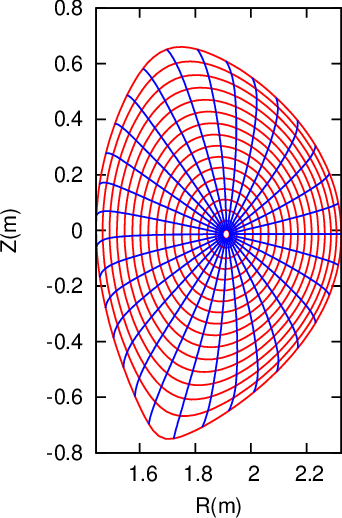
\includegraphics{/home/yj/project_new/read_gfile/fig161/out1.eps}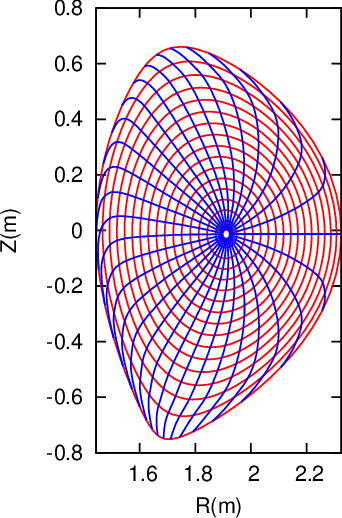
\includegraphics{/home/yj/project_new/read_gfile/fig161/out2.eps}
  \caption{\label{8-23-1}The equal-arc poloidal angle (left) and the
  straight-line poloidal angle (right) for EAST equilibrium \#38300@3.9s. The
  blue lines correspond to the equal-$\theta$ lines, with uniform $\theta$
  interval between neighbour lines. The red lines correspond to the magnetic
  surfaces, which start from $\sqrt{\overline{\Psi}_t} = 0.01714$ (the
  innermost magnetic surface) and end at $\sqrt{\overline{\Psi}_t} = 0.9851$
  (the boundary magnetic surface), and are equally spaced in
  $\sqrt{\overline{\Psi}_t}$.}
\end{figure}

\subsubsection{Verification of Jacobian}

After the magnetic coordinates are constructed, we can evaluate the Jacobian
$\mathcal{J}_{\tmop{new}}$ by using directly the definition of the Jacobian,
i.e.,
\begin{equation}
  \mathcal{J}_{\tmop{new}} = \frac{1}{(\nabla \psi \times \nabla
  \overline{\theta}) \cdot \nabla \phi},
\end{equation}
which can be further written as
\begin{equation}
  \mathcal{J}_{\tmop{new}} = R (R_{\overline{\theta}} Z_{\psi} - R_{\psi}
  Z_{\overline{\theta}}),
\end{equation}
where the partial differential can be evaluated by using numerical
differential schemes. The results obtained by this way should agree with
results obtained from the analytical form of the Jacobian. This consistency
check provide a verification for the correctness of the theory derivation and
numerical implementation. In evaluating the Jacobian by using the analytical
form, we may need to evaluate $\nabla \psi$, which finally reduces to
evaluating $\nabla \Psi$. The value of $| \nabla \Psi |$ is obtained
numerically based on the numerical data of $\Psi$ given in cylindrical
coordinate grids. Then the cubic spline interpolating formula is used to
obtain the value of $| \nabla \Psi |$ at desired points.
($\mathcal{J}_{\tmop{new}}$ calculated by the second method (i.e. using
analytic form) is used in the GTAW code; the first methods are also
implemented in the code for the benchmark purpose.) In the following sections,
for notation ease, the Jacobiban of the constructed coordinate system will be
denoted by $\mathcal{J}$, rather than $\mathcal{J}_{\tmop{new}}$.

\subsubsection{Radial coordinate}\label{9-27-1}

The radial coordinate $\psi$ can be chosen to be various surface function,
e.g., volume, poloidal or toroidal magnetic flux within a magnetic surface.
The frequently used radial coordinates include $\overline{\Psi}$, and
$\sqrt{\overline{\Psi}}$, where $\overline{\Psi}$ is defined by
\begin{equation}
  \label{19-4-11-3} \overline{\Psi} = \frac{\Psi - \Psi_0}{\Psi_a - \Psi_0},
\end{equation}
where $\Psi_0$ and $\Psi_a$ are the values of $\Psi$ at the magnetic axis and
LCFS, respectively. Other choices of the radial coordinates: the toroidal
magnetic flux and its square root, $\overline{\Psi}_t$, and
$\sqrt{\overline{\Psi}_t}$, where $\Psi_t$ and $\overline{\Psi}_t$ are defined
by
\begin{equation}
  \frac{d \Psi_t}{d \Psi} = 2 \pi q, \Psi_t (0) = 0
\end{equation}
and
\begin{equation}
  \overline{\Psi}_t = \frac{\Psi_t}{\Psi_t (1)},
\end{equation}
respectively, where $\Psi_t (0)$ and $\Psi_t (1)$ are the values of $\Psi_t$
at the magnetic axis and LCFS, respectively.

If $\psi = \sqrt{\overline{\Psi}_t}$, then
\begin{equation}
  \frac{d \Psi}{d \psi} = \frac{d \Psi}{d \Psi_t}  \frac{d \Psi_t}{d \psi} =
  \frac{1}{2 \pi q}  \frac{d \Psi_t}{d \psi} = \frac{1}{2 \pi q}  \frac{d
  \Psi_t}{d \overline{\Psi_t}}  \frac{d \overline{\Psi}_t}{d \psi} =
  \frac{1}{2 \pi q} \Psi_t (1) 2 \psi
\end{equation}
The cylindrical coordinates $(R, \phi, Z)$ is a right-hand system, with the
positive direction of $Z$ pointing vertically up. In GTAW code, the positive
direction of $\theta$ is chosen in the anticlockwise direction when observers
look along the direction of $\hat{\tmmathbf{\phi}}$. Then the definition
$\mathcal{J}^{- 1} = \nabla \psi \times \nabla \theta \cdot \nabla \phi$
indicates that (1) $\mathcal{J}$ is negative if $\nabla \psi$ points from the
magnetic axis to LCFS; (2) $\mathcal{J}$ is positive if $\nabla \psi$ points
from the LCFS to the magnetic axis. This can be used to determine the sign of
Jacobian after using the analytical formula to obtain the absolute value of
Jacobian.

If $\psi = \overline{\Psi}$ or $\psi = \sqrt{\overline{\Psi}}$, $\nabla \psi$
points from the magnetic axis to LCFS.

The volume between magnetic surfaces can also be used as a radial coordinate.
The differential volume element is written as
\begin{equation}
  d^3 V = \mathcal{J} d \psi d \theta d \phi .
\end{equation}
Integrating over the toroidal angle, we obtain
\begin{equation}
  d^2 V = 2 \pi \mathcal{J} d \psi d \theta
\end{equation}
Further integrating over the poloidal angle, we obtain
\begin{equation}
  d^1 V = 2 \pi d \psi \oint \mathcal{J} d \theta,
\end{equation}
i.e.,
\begin{equation}
  \frac{d^1 V}{d \psi} = 2 \pi \oint \mathcal{J} d \theta .
\end{equation}
In codes I wrote, I stick to using $\overline{\Psi}$ as the radial coordinate
when doing computation, and transform to other radial coordinates when
presenting the results if needed.

\

\section{Constructing magnetic surface coordinate system from discrete $\Psi
(R, Z)$ data}\label{6-25-1}

Given an axisymmetric tokamak equilibrium in $(R, \phi, Z)$ coordinates (e.g.,
2D data $\Psi (R, Z)$ on a rectangular grids $(R, Z)$ in G-file), we can
construct a magnetic surface coordinates $(\psi, \theta, \phi)$ by the
following two steps. (1) Find out a series of magnetic surfaces on $(R, Z)$
plane and select radial coordinates for each magnetic surface (e.g. the
poloidal flux within each magnetic surface). (2) Specify the Jacobian or some
property that we want the poloidal angle to have. Then calculate the poloidal
angle of each point on each flux surface (on the $\phi = \tmop{const}$ plane)
by using Eq. (\ref{5-30-p1}) (if the Jacobian is specified) or some method
specified by us to achieve some property we prefer for the poloidal angle (if
a Jacobian is not directly specified). Then we obtain the magnetic surface
coordinates system $(\psi, \theta, \phi)$.

\subsection{Finding magnetic surfaces}

Two-dimensional data $\Psi (R, Z)$ on a rectangular grids $(R, Z)$ is read
from the G\_EQDSK file (G-file) of EFIT code. Based on the 2D array data, I
use 2D cubic spline interpolation to construct a interpolating function $\Psi
= \Psi (R, Z)$. To construct a magnetic surface coordinate system, I need to
find the contours of $\Psi$, i.e., magnetic surfaces. The values of $\Psi$ on
the magnetic axis, $\Psi_0$, and the value of $\Psi$ on the last closed flux
surface (LCFS), $\Psi_b$, are given in G-file. Using these two values, I
construct a 1D array ``psival'' with value of elements changing uniform from
$\Psi_0$ to $\Psi_b$. Then I try to find the contours of $\Psi$ with contour
level value ranging from $\Psi_0$ to $\Psi_b$. This is done in the following
way: construct a series of straight line (in the poloidal plane) that starts
from the location of the magnetic axis and ends at one of the points on the
LCFS. Combine the straight line equation, $Z = Z (R)$, with the interpolating
function $\Psi (R, Z)$, we obtain a one variable function $h = \Psi (R, Z
(R))$. Then finding the location where $\Psi$ is equal to a specified value
$\Psi_i$, is reduced to finding the root of the equation $\Psi (R, Z (R)) -
\Psi_i = 0$. Since this is a one variable equation, the root can be easily
found by using simple root finding scheme, such as bisection method (bisection
method is used in GTAW code). After finding the roots for each value in the
array ``psival'' on each straight lines, the process of finding the contours
of $\Psi$ is finished. The contours of $\Psi$ found this way are plotted in
Fig. \ref{4-3-p2}.

\

\begin{figure}[h]
  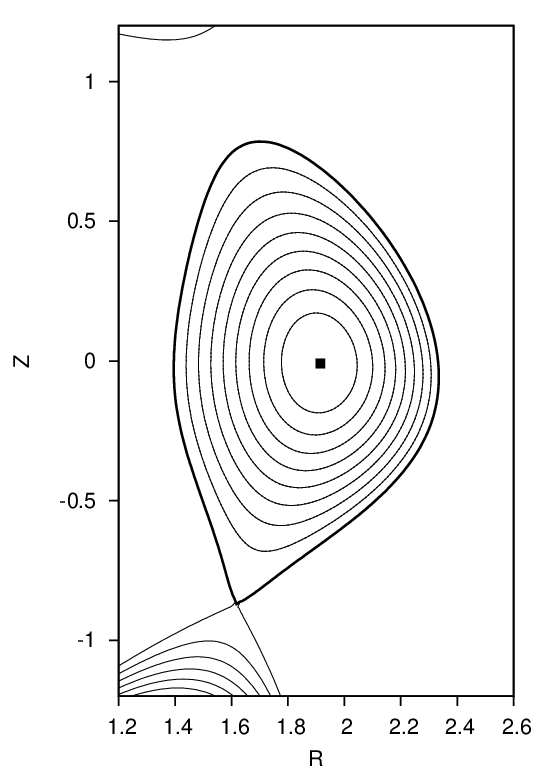
\includegraphics{/home/yj/project_new/read_gfile/fig1/contour.eps}
  \caption{\label{4-3-p2}Verification of the numerical code that calculates
  the contours of the poloidal flux $\Psi$. The bold line in the figure
  indicates the LCFS. The contour lines (solid lines) given by the gnuplot
  program agrees well with the results I calculate by using interpolation and
  root-finding method (the two sets of contours are indistinguishable in this
  scale). My code only calculate the contour lines within the LCFS, while
  those given by gnuplot contains additional contour lines below the X point
  and on the left top in the figure. Eqdisk file of the equilibrium was
  provided by Dr. Guoqiang Li (filename: g013606.07104).}
\end{figure}

\

In the above, we mentioned that the point of magnetic axis and points on the
LCFS are needed to construct the straight lines. In G-file, points on LCFS are
given explicitly in an array. The location of magnetic axis is also explicitly
given in G-file. It is obvious that some of the straight lines $Z = Z (R)$
that pass through the location of magnetic axis and points on the LCFS will
have very large or even infinite slope. On these lines, finding the accurate
root of the equation $\Psi (R, Z (R)) - \Psi_i = 0$ is difficult or even
impossible. The way to avoid this situation is obvious: switch to use function
$R = R (Z)$ instead of $Z = Z (R)$ when the slope of $Z = Z (R)$ is large (the
switch condition I used is $|d Z / d R| > 1$).

In constructing the flux surface coordinate with desired Jacobian, we will
need the absolute value of the gradient of $\Psi$, $| \nabla \Psi |$, on some
specified spatial points. To achieve this, we need to construct a
interpolating function for $| \nabla \Psi |$. The $| \nabla \Psi |$ can be
written as
\begin{equation}
  | \nabla \Psi | = \sqrt{\left( \frac{\partial \Psi}{\partial R} \right)^2 +
  \left( \frac{\partial \Psi}{\partial Z} \right)^2},
\end{equation}
By using the center difference scheme to evaluate the partial derivatives with
respect to $R$ and $Z$ in the above equation (using one side difference scheme
for the points on the rectangular boundary), we can obtain an 2D array for the
value of $| \nabla \Psi |$ on the rectangular $(R, Z)$ grids. Using this 2D
array, we can construct an interpolating function for $\nabla \Psi$ by using
the cubic spline interpolation scheme.

\begin{figure}[h]
  \includegraphics{/home/yj/project_new/read_gfile/fig2/plt.eps}\includegraphics{/home/yj/project_new/read_gfile/fig40/plt.eps}
  \caption{Grid points (the intersecting points of two curves in the figure)
  corresponding to uniform poloidal flux and uniform poloidal arc length for
  EAST equilibrium shot 13606 at 7.1s (left) (G-file name: g013606.07104) and
  shot 38300 at 3.9s (right) (G-file name: g038300.03900).}
\end{figure}

\begin{figure}[h]
  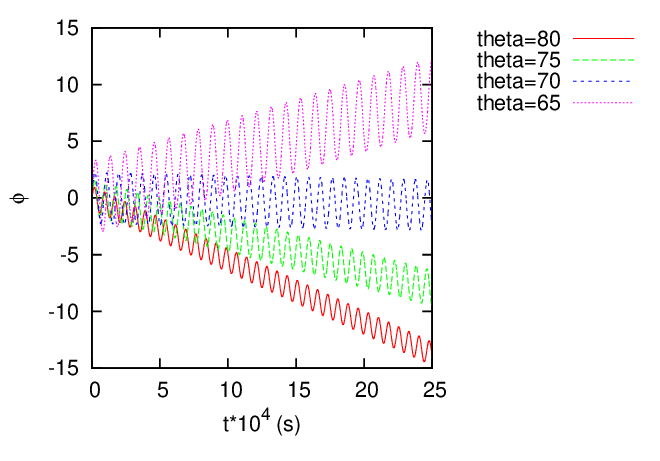
\includegraphics{/home/yj/project_new/read_gfile/fig41/p2.eps}
  \caption{$| \nabla \Psi |$ as a function of the poloidal angle. The
  different lines corresponds to the values of $| \nabla \Psi |$ on different
  magnetic surfaces. The stars correspond to the values on the boundary
  magnetic surface while the plus signs correspond to the value on the
  innermost magnetic surface (the magnetic surface adjacent to the magnetic
  axis). The equilibrium is for EAST shot 38300 at 3.9s.}
\end{figure}

\begin{figure}[h]
  \resizebox{0.4\columnwidth}{!}{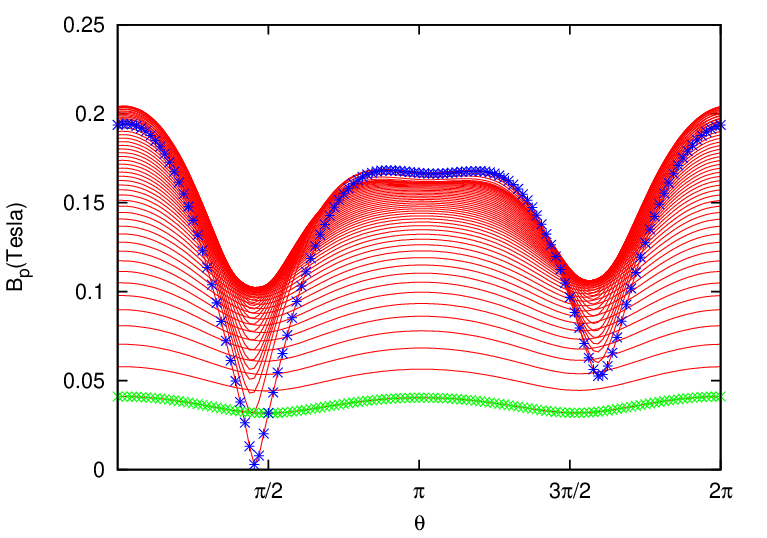
\includegraphics{/home/yj/project_new/read_gfile/fig41/p3.eps}}\resizebox{0.4\columnwidth}{!}{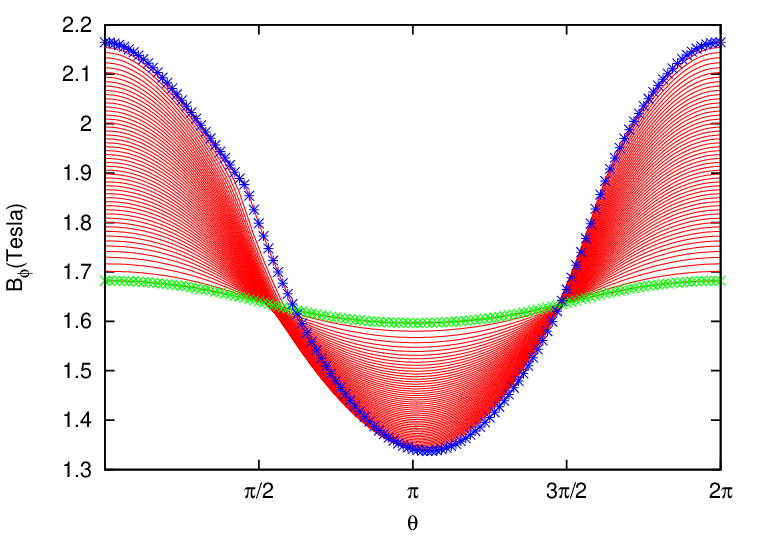
\includegraphics{/home/yj/project_new/read_gfile/fig41/p4.eps}}
  \caption{The Poloidal magnetic field $B_p = | \nabla \Psi | / R$ (left) and
  toroidal magnetic field $B_{\phi} = g / R$ (right) as a function of the
  poloidal angle. The different lines corresponds to the values on different
  magnetic surfaces. The stars correspond to the values on the boundary
  magnetic surface while the plus signs correspond to the value on the
  innermost magnetic surface (the magnetic surface adjacent to the magnetic
  axis). The equilibrium is for EAST shot 38300 at 3.9s.}
\end{figure}

\

\

\begin{figure}[h]
  \includegraphics{/home/yj/project_new/read_gfile/fig41/tmp.eps}
  \caption{Equal-arc Jacobian as a function of the poloidal angle on different
  magnetic surfaces. The dotted line corresponds to the values of Jacobian on
  the boundary magnetic surface. The equilibrium is for EAST shot 38300 at
  3.9s.}
\end{figure}

\begin{figure}[h]
  \includegraphics{/home/yj/project_new/read_gfile/fig32/tmp.eps}
  \caption{$| \nabla \Psi |$ as a function of the poloidal angle. The
  different lines corresponds to values of $| \nabla \Psi |$ on different
  magnetic surfaces. The stars correspond to the values of $| \nabla \Psi |$
  on the boundary magnetic surface while the plus signs correspond to the
  value on the innermost magnetic surface (the magnetic surface adjacent to
  the magnetic axis). The equilibrium is a Solovev equilibrium.}
\end{figure}

\

\begin{figure}[h]
  \includegraphics{/home/yj/project_new/read_gfile/fig29/tmp.eps}
  \caption{Jacobian on different magnetic surfaces as a function of the
  poloidal angle. The equilibrium is a Solovev equilibrium and the Jacobian is
  an equal-arc Jacobian. The stars correspond to the values of Jacobian on the
  boundary magnetic surface while the plus signs correspond to the value on
  the innermost magnetic surface (the magnetic surface adjacent to the
  magnetic axis).}
\end{figure}

\

\subsection{Expression of metric elements of magnetic coordinates $(\psi,
\theta, \phi)$}

Metric elements of the $(\psi, \theta, \phi)$ coordinates, e.g., $\nabla \psi
\cdot \nabla \theta$, are often needed in practical calculations. Next, we
express these metric elements in terms of the cylindrical coordinates $(R, Z)$
and their partial derivatives with respect to $\psi$ and $\theta$. Note that,
in this case, the coordinate system is $(\psi, \theta, \phi)$ while $R$ and
$Z$ are functions of $\psi$ and $\theta$, i.e.,
\begin{equation}
  R = R (\psi, \theta),
\end{equation}
\begin{equation}
  Z = R (\psi, \theta) .
\end{equation}
Then $\nabla R$ and $\nabla Z$ are written as
\begin{equation}
  \label{4-19-e10} \nabla R = \hat{\mathbf{R}} = R_{\psi} \nabla \psi +
  R_{\theta} \nabla \theta,
\end{equation}
\begin{equation}
  \label{4-19-e11} \nabla Z = \hat{\mathbf{Z}} = Z_{\psi} \nabla \psi +
  Z_{\theta} \nabla \theta,
\end{equation}
wehre $R_{\psi} \equiv \partial R / \partial \psi$, etc. Equations
(\ref{4-19-e10}) and (\ref{4-19-e11}) can be solved to give
\begin{equation}
  \label{4-19-e2} \nabla \psi = \frac{1}{R_{\psi} Z_{\theta} - Z_{\psi}
  R_{\theta}} (Z_{\theta} \hat{\mathbf{R}} - R_{\theta} \hat{\mathbf{Z}}),
\end{equation}
\begin{equation}
  \label{4-19-e3} \nabla \theta = \frac{1}{Z_{\psi} R_{\theta} - R_{\psi}
  Z_{\theta}} (Z_{\psi} \hat{\mathbf{R}} - R_{\psi} \hat{\mathbf{Z}}) .
\end{equation}
Using the above expressions, the Jacobian of $(\psi, \theta, \phi)$
coordinates, $\mathcal{J}$, is written as
\begin{eqnarray}
  \mathcal{J}^{- 1} & = & \nabla \psi \times \nabla \theta \cdot \nabla \phi
  \nonumber\\
  & = & - \frac{1}{(R_{\psi} Z_{\theta} - Z_{\psi} R_{\theta})^2} (Z_{\theta}
  R_{\psi} \hat{\tmmathbf{\phi}} - R_{\theta} Z_{\psi} \hat{\tmmathbf{\phi}})
  \times \frac{\hat{\tmmathbf{\phi}}}{R} \nonumber\\
  & = & - \frac{1}{(Z_{\theta} R_{\psi} - R_{\theta} Z_{\psi}) R}, 
\end{eqnarray}
i.e.,
\begin{equation}
  \label{4-19-e1} \mathcal{J}= R (R_{\theta} Z_{\psi} - R_{\psi} Z_{\theta}) .
\end{equation}
Using this, Expressions (\ref{4-19-e2}) and (\ref{4-19-e3}) are written as
\begin{equation}
  \label{6-9-e1} \nabla \psi = - \frac{R}{\mathcal{J}} (Z_{\theta}
  \hat{\mathbf{R}} - R_{\theta} \hat{\mathbf{Z}})
\end{equation}
and
\begin{equation}
  \label{6-9-e2} \nabla \theta = \frac{R}{\mathcal{J}} (Z_{\psi}
  \hat{\mathbf{R}} - R_{\psi} \hat{\mathbf{Z}}) .
\end{equation}
Then the elements of the metric matrix are written as
\begin{equation}
  \label{4-19-e7} | \nabla \psi |^2 = \frac{R^2}{\mathcal{J}^2} (Z_{\theta}^2
  + R_{\theta}^2),
\end{equation}
\begin{equation}
  \label{4-19-e8} | \nabla \theta |^2 = \frac{R^2}{\mathcal{J}^2} (Z_{\psi}^2
  + R_{\psi}^2),
\end{equation}
and
\begin{equation}
  \label{4-19-e9} \nabla \psi \cdot \nabla \theta = -
  \frac{R^2}{\mathcal{J}^2} (Z_{\theta} Z_{\psi} + R_{\theta} R_{\psi}) .
\end{equation}
Equations (\ref{4-19-e7}), (\ref{4-19-e8}), and (\ref{4-19-e9}) are the
expressions of the metric elements in terms of $R$, $R_{\psi}$, $R_{\theta}$,
$Z_{\psi}$, and $Z_{\theta}$. [Combining the above results, we obtain
\begin{equation}
  \label{11-11-1} \frac{\nabla \psi \cdot \nabla \theta}{| \nabla \psi |^2} =
  - \frac{Z_{\theta} Z_{\psi} + R_{\theta} R_{\psi}}{Z_{\theta}^2 +
  R_{\theta}^2} .
\end{equation}
Equation (\ref{4-19-e9}) is used in GTAW code. Using the above results,
$h^{\alpha \beta} = \frac{\mathcal{J}}{R^2} \nabla \alpha \cdot \nabla \beta$
are written as
\begin{equation}
  h^{\psi \psi} = \frac{\mathcal{J}}{R^2} | \nabla \psi |^2 =
  \frac{1}{\mathcal{J}} (Z_{\theta}^2 + R_{\theta}^2)
\end{equation}
\begin{equation}
  h^{\theta \theta} = \frac{\mathcal{J}}{R^2} | \nabla \theta |^2 =
  \frac{1}{\mathcal{J}} (Z_{\psi}^2 + R_{\psi}^2),
\end{equation}
\begin{equation}
  h^{\psi \theta} = \frac{\mathcal{J}}{R^2} \nabla \psi \cdot \nabla \theta =
  - \frac{1}{\mathcal{J}} (Z_{\theta} Z_{\psi} + R_{\theta} R_{\psi})
\end{equation}
As a side product of the above results, we can calculate the arc length in the
poloidal plane along a constant $\psi$ surface, $d \ell_p$, which is expressed
as
\begin{eqnarray*}
  d \ell_p & = & \sqrt{(d R)^2 + (d Z)^2}\\
  & = & \sqrt{(R_{\psi} d \psi + R_{\theta} d \theta)^2 + (Z_{\psi} d \psi +
  Z_{\theta} d \theta)^2} .
\end{eqnarray*}
Note that $d \psi = 0$ since we are considering the arc length along a
constant $\psi$ surface in $(R, Z)$ plane. Then the above expression is
reduced to
\begin{eqnarray}
  d \ell_p & = & \sqrt{(R_{\theta} d \theta)^2 + (Z_{\theta} d \theta)^2}
  \nonumber\\
  & = & \sqrt{R_{\theta}^2 + Z_{\theta}^2} d \theta \nonumber\\
  & = & \frac{|\mathcal{J} \nabla \psi |}{R} d \theta,  \label{6-8-e1}
\end{eqnarray}
which agrees with Eq. (\ref{5-30-p1}).]

\section{Constructing model tokamak magnetic field}

In some cases (e.g., turbulence simulation), model tokamak magnetic field,
which is not an exact solution to the GS equation, is often used. In the
model, the safety factor profile $q (\psi)$, toroidal field function $g
(\psi)$, and the magnetic surface shape $(R (\psi, \theta), Z (\psi, \theta))$
are given. To use this model in a simulation, we need to calculate its
poloidal magnetic field, which is determined by the poloidal magnetic flux
function $\Psi$. To determine $\Psi$, we need to use Eq. (\ref{7-11-p1}),
i.e.,
\begin{equation}
  q (\psi) = - \frac{1}{2 \pi}  \frac{g}{\Psi'} \int_0^{2 \pi}
  \frac{\mathcal{J}}{R^2} d \theta,
\end{equation}
and re-organize the formula as
\begin{equation}
  \frac{d \Psi}{d \psi} = - \frac{1}{2 \pi}  \frac{g (\psi)}{q (\psi)}
  \int_0^{2 \pi} \frac{\mathcal{J}}{R^2} d \theta,
\end{equation}
which can be integrated to obtain $\Psi$ and thus the poloidal magnetic field
$\mathbf{B}_p = \nabla \Psi \times \nabla \phi$, where $\mathcal{J} = [(\nabla
\psi \times \nabla \theta) \cdot \nabla \phi]^{- 1}$. The toroidal magnetic
field can be obtained from $g (\psi)$ by $B_{\phi} = g / R$. In most papers,
$g (\psi)$ is chosen to be a constant.

A typical magnetic surface shape used in simulations is the Miller shape,
which is given by
\begin{equation}
  \begin{array}{l}
    R (r, \theta) = R_0 (r) + r \cos [\theta + (\sin^{- 1} \delta (r)) \sin
    \theta]\\
    Z (r, \theta) = \kappa (r) r \sin \theta
  \end{array}
\end{equation}
where $r = \psi$ is the radial coordinate, $R_0 (r)$, $\delta (r)$, and
$\kappa_r (r)$ are the Shafronov shift, triangularity, and elongation
profiles, which can be arbitrarily specified. For the special case of $R_0$
being a constant, $\delta (r) = 0$, and $\kappa (r) = 1$, this shape reduces
to a concentric-circular magnetic field. An example of calculating the
poloidal field of the model field is given in Sec. \ref{19-4-8-p1}. This kind
of model field can be called theoretical physicists' tokamak. Computational
physicists often use this model for code benchmarking purpose. The famous
DIII-D cyclone base case is an example, which was extensively used for
benchmarking gyrokinetic simulation of ion temperature driven turbulence.

\section{Magnetic surface averaging}

\subsection{Definition}

The magnetic surface average of a physical quantity $G (\psi, \theta, \phi)$
is defined by
\begin{equation}
  \label{6-14-2} \langle G \rangle \equiv \lim_{\Delta \Psi \rightarrow 0}
  \left( \frac{\int \int \int_{\Delta \Psi} G d^3 V}{\int \int \int_{\Delta
  \Psi} d^3 V} \right),
\end{equation}
where the volume integration is over a small volume between two adjacent flux
surfaces with $\Psi$ differing by $\triangle \Psi$. [This formula (with finite
$\Delta \Psi$) is used in \tmtexttt{TEK} code to calculate the radial heat
flux.]

The above 3D volume integration can also be written as a 2D surface
integration. The differential volume element is given by $d^3 V = |
\mathcal{J} | d \psi d \theta d \phi$, where $\mathcal{J}$ is the Jacobian of
$(\psi, \theta, \phi)$ coordinates. Using this, equation (\ref{6-14-2}) is
written as
\begin{eqnarray}
  \langle G \rangle & = & \lim_{\Delta \Psi \rightarrow 0} \left( \frac{\int
  \int \int_{\Delta \Psi} G | \mathcal{J} | d \psi d \theta d \phi}{\int \int
  \int_{\Delta \Psi} | \mathcal{J} | d \psi d \theta d \phi} \right)
  \nonumber\\
  & = & \frac{\int \int G | \mathcal{J} | d \theta d \phi}{\int \int |
  \mathcal{J} | d \theta d \phi},  \label{23-1-4-1}
\end{eqnarray}
which is a 2D averaging over a magnetic surface and thus is called magnetic
surface average. Note that the surface averaging of any $n \neq 0$ harmonic is
zero ($n$ is the toroidal mode number). Therefore the magnetic surface average
contains only the contribution from the $n = 0$ component, i.e., axisymmetric
component. (On the other hand, $m \neq 0$ poloidal harmonics of $G$ can
contribute to the surface average since the Jacobian has a poloidal angle
dependence.) Using this and noting that $\mathcal{J}$ is axisymmetric, then
expression (\ref{23-1-4-1}) is written as
\begin{equation}
  \langle G \rangle = \frac{\int G_0 (\psi, \theta) | \mathcal{J} | d
  \theta}{\int | \mathcal{J} | d \theta},
\end{equation}
where $G_0 (\theta)$ is defined by the following Fourier expansion:
\begin{equation}
  G = \sum_{n = - \infty}^{+ \infty} G_n (\psi, \theta) \exp (- i n \phi) .
\end{equation}


\hrulefill

``Zonal'' and ``mean'' components

$\langle G \rangle$ is sometimes called the ``zonal'' component of $G$ if the
radial wavelength of $\langle G \rangle$ is much smaller than the equilibrium
scale length. If the radial wavelength of $\langle G \rangle$ is comparable to
the equilibrium scale length, $\langle G \rangle$ is usually called ``mean''
component in tokamak literature. For example, mean flows are of system space
scale and thus are easy to be observed in experiments. On the other hand, the
``zonal'' flow, which usually refers to the turbulence generated secondary
flow, is of much smaller radial scale (the radial wavelength of zonal flow is
of several Larmor radius) and thus is difficult to observe in experiments.

\hrulefill

Sometimes, we do not want the Jacobian to explicitly appear in the formula.
This can be achieved by writing the differential volume element as
\begin{equation}
  \label{6-14-1} d^3 V = R d \phi \frac{d \Psi}{| \nabla \Psi |} d l_p .
\end{equation}
Using $B_p = | \nabla \Psi | / R$, the volume element is further written as
\begin{equation}
  d^3 V = d \phi \frac{d \Psi}{B_p} d l_p
\end{equation}
Using this, the averaging defined in Eq. (\ref{6-14-2}) is written as
\begin{eqnarray}
  \langle G \rangle & = & \lim_{\Delta \Psi \rightarrow 0} \frac{\int \int
  \int_{\Delta \Psi} G d \phi \frac{d \Psi}{B_p} d l_p}{\int \int \int_{\Delta
  \Psi} d \phi \frac{d \Psi}{B_p} d l_p} \nonumber\\
  & = & \frac{\int \int G \frac{1}{B_p} d \phi d l_p}{\int \int \frac{1}{B_p}
  d \phi d l_p} . 
\end{eqnarray}
If $G$ is axisymmetric, then the above equation is written as
\begin{equation}
  \label{10-16-3} \langle G \rangle = \frac{\oint G \frac{1}{B_p} d l_p}{\oint
  \frac{1}{B_p} d l_p} .
\end{equation}
(Equation (\ref{10-16-3}) is used in the GTAW code to calculate the magnetic
surface averaging.) Using Eq. (\ref{5-30-p1}) and $B_p = | \nabla \Psi | / R$,
equation (\ref{10-16-3}) can also be written as
\begin{equation}
  \label{3-18-a1m} \langle G \rangle = \frac{\int_0^{2 \pi} G |\mathcal{J}| d
  \theta}{\int_0^{2 \pi} |\mathcal{J}| d \theta} .
\end{equation}
Using the expression of the volume element $d \tau = |\mathcal{J}| d \theta d
\phi d \psi$, the volume within a magnetic surface is written
\begin{equation}
  \label{4-18-3} V (\psi) = \int d \tau = \int |\mathcal{J}| d \theta d \phi d
  \psi = 2 \pi \int_{\psi_0}^{\psi} \int_0^{2 \pi} |\mathcal{J}| d \theta d
  \psi .
\end{equation}
Using this, the differential of $V$ with respect to $\psi$ is written as
\begin{equation}
  \label{4-7-p1} V' \equiv \frac{d V}{d \psi} = 2 \pi \int_0^{2 \pi}
  |\mathcal{J}| d \theta .
\end{equation}
Using this, Eq. (\ref{3-18-a1m}) is written as
\[ \langle G \rangle = \frac{2 \pi}{V'} \int_0^{2 \pi} G |\mathcal{J}| d
   \theta \]


\subsection{Flux Surface Functions---to be deleted}\label{7-25-e1}

Next, examine the meaning of the following volume integral
\begin{equation}
  D (\psi) \equiv \int_V \mathbf{B} \cdot \nabla \theta d \tau,
\end{equation}
where the volume $V = V (\psi)$ is the volume within the magnetic surface
labeled by $\psi$. Using $\nabla \cdot \mathbf{B}= 0$, the quantity $D$ can be
further written as
\begin{equation}
  \label{4-17-p1} D = \int_V \nabla \cdot (\theta \mathbf{B}) d \tau .
\end{equation}
Note that $\theta$ is not a single-value function of the spacial points. In
order to evaluate the integration in Eq. (\ref{4-17-p1}), we need to select
one branch of $\theta$, which can be chosen to be $0 \leqslant \theta < 2
\pi$. Note that function $\theta = \theta (R, Z)$ is not continuous in the
vicinity of the contour of $\theta = 0$. Next, we want to use the Gauss's
theorem to convert the above volume integration to surface integration. Noting
the discontinuity of the integrand $\theta \mathbf{B}$ in the vicinity of the
contour of $\theta = 0$, the volume should be cut along the contour, thus,
generating two surfaces. Denote these two surfaces by $S_1$ and $S_2$, then
equation (\ref{4-17-p1}) is written as
\begin{eqnarray*}
  D & = & \int_{S_1} \theta \mathbf{B} \cdot d\mathbf{S}+ \int_{S_2} \theta
  \mathbf{B} \cdot d\mathbf{S}+ \int_{S_3} \theta \mathbf{B} \cdot
  d\mathbf{S},
\end{eqnarray*}
where the direction of surface $S_1$ is in the negative direction of $\theta$,
the direction of $S_2$ is in the positive direction of $\theta$, and the
surface $S_3$ is the toroidal magnetic surface $\psi = \psi_0$. The surface
integration through $S_3$ is obviously zero since $\mathbf{B}$ lies in this
surface. Therefore, we have
\begin{eqnarray}
  D & = & \int_{S_1} \theta \mathbf{B} \cdot d\mathbf{S}+ \int_{S_2} \theta
  \mathbf{B} \cdot d\mathbf{S}+ 0 \nonumber\\
  & = & \int_{S_1} 0\mathbf{B} \cdot d\mathbf{S}+ \int_{S_2} 2 \pi \mathbf{B}
  \cdot d\mathbf{S} \nonumber\\
  & = & 2 \pi \int_{S_2} \mathbf{B} \cdot d\mathbf{S}.  \label{4-18-4}
\end{eqnarray}
Eq. (\ref{4-18-4}) indicates that $D$ is $2 \pi$ times the magnetic flux
through the $S_2$ surface. Thus, the poloidal flux through $S_2$ is written as
\begin{equation}
  \Psi_p = \frac{1}{2 \pi} D = \frac{1}{2 \pi} \int_V \mathbf{B} \cdot \nabla
  \theta d \tau .
\end{equation}
Using the expression of the volume element $d \tau = |\mathcal{J}| d \theta d
\phi d \psi$, $\Psi_p$ can be further written in terms of flux surface
averaged quantities.
\begin{eqnarray}
  \Psi_p & = & \frac{1}{2 \pi} \int_V \mathbf{B} \cdot \nabla \theta
  |\mathcal{J}| d \theta d \phi d \psi \nonumber\\
  & = & \int_0^{\psi} d \psi \int_0^{2 \pi} \mathbf{B} \cdot \nabla \theta
  |\mathcal{J}| d \theta \nonumber\\
  & = & \int_0^{\psi} d \psi \int_0^{2 \pi} \Psi' \nabla \psi \times \nabla
  \phi \cdot \nabla \theta |\mathcal{J}| d \theta \nonumber\\
  & = & - \tmop{sign} (\mathcal{J}) \int_0^{\psi} d \psi \int_0^{2 \pi} \Psi'
  (\psi) d \theta \nonumber\\
  & = & - 2 \pi \tmop{sign} (\mathcal{J}) \int_0^{\psi} \Psi' (\psi) d \psi
  \nonumber\\
  & = & - 2 \pi \tmop{sign} (\mathcal{J}) [\Psi (\psi) - \Psi (0)] . 
  \label{4-10-p11}
\end{eqnarray}
Note that the sign of the Jacobian appears in Eq. (\ref{4-10-p11}), which is
due to the positive direction of surface $S_2$ is determined by the positive
direction of $\theta$, which in turn is determined by the sign of the Jacobian
(In my code, however, the positive direction of $\theta$ is chosen by me and
the sign of the Jacobian is determined by the positive direction of $\theta$).
We can verify the sign of Eq. (\ref{4-10-p11}) is exactly consistent with that
in Eq. (\ref{12-30-2}).

Similarly, the toroidal flux within a flux surface is written as
\begin{equation}
  \Psi_t = \frac{1}{2 \pi} \int_V \mathbf{B} \cdot \nabla \phi d \tau,
\end{equation}
the poloidal current within a flux surface is written as
\begin{equation}
  K (\psi) = \frac{1}{2 \pi} \int_V \mathbf{J} \cdot \nabla \theta d \tau,
\end{equation}
and toroidal current within a flux surface is written as
\begin{equation}
  \label{4-18-1} I (\psi) = \frac{1}{2 \pi} \int_V \mathbf{J} \cdot \nabla
  \phi d \tau .
\end{equation}
(**check**)The toroidal magnetic flux is written as
\begin{eqnarray}
  \Psi_t & = & \frac{1}{2 \pi} \int \mathbf{B} \cdot \nabla \phi |\mathcal{J}|
  d \theta d \phi d \psi \nonumber\\
  & = & \int_0^{\psi} d \psi \int_0^{2 \pi} g \frac{1}{R^2} |\mathcal{J}| d
  \theta \nonumber\\
  & = & \int_0^{\psi} \left[ g \frac{V'}{2 \pi} \left\langle \frac{1}{R^2}
  \right\rangle \right] d \psi .  \label{4-7-p3}
\end{eqnarray}
\[ \Rightarrow \Psi_t' = g \frac{V'}{2 \pi} \left\langle \frac{1}{R^2}
   \right\rangle \]
\[ \Rightarrow \frac{d \Psi_t}{d V} = g \frac{1}{2 \pi} \left\langle
   \frac{1}{R^2} \right\rangle \]
\begin{equation}
  \Rightarrow \frac{d \Psi}{d V} = \frac{g}{2 \pi q}  \frac{1}{2 \pi}
  \left\langle \frac{1}{R^2} \right\rangle .
\end{equation}
Next, calculate the derivative of the toroidal flux with respect to the
poloidal flux.
\begin{eqnarray}
  \frac{d \Psi_t}{d \Psi_p} & = & \frac{\Psi_t'}{\Psi_p'} \nonumber\\
  & = & - \frac{g V'}{(2 \pi)^2 \Psi'}  \left\langle \frac{1}{R^2}
  \right\rangle,  \label{4-18-6}
\end{eqnarray}
Comparing this result with Eq. (\ref{12-21-p2}) indicates that it is equal to
the safety factor, i.e.,
\begin{equation}
  \label{5-14-3} \frac{d \Psi_t}{d \Psi_p} = q (\psi) .
\end{equation}
By using the contravariant representation of current density (\ref{4-16-p2}),
the poloidal current within a magnetic surface is written as
\begin{eqnarray}
  K (\psi) & = & \frac{1}{2 \pi} \int \mathbf{J} \cdot \nabla \theta
  \mathcal{J}d \theta d \phi d \psi \nonumber\\
  & = & \frac{1}{\mu_0} \int (- g') \nabla \phi \times \nabla \psi \cdot
  \nabla \theta \mathcal{J}d \theta d \psi \nonumber\\
  & = & - \frac{1}{\mu_0} \int g' d \theta d \psi \nonumber\\
  & = & - \frac{2 \pi}{\mu_0} \int_0^{\psi} g' d \psi \nonumber\\
  & = & - \frac{2 \pi}{\mu_0} [g (\psi) - g (0)] . 
\end{eqnarray}
Note that the poloidal current is proportional to $g$, which explains why $g$
is sometimes called poloidal current function in tokamak literature.
\[ - \left[ \left( \Psi' \frac{\mathcal{J}}{R^2} | \nabla \psi |^2
   \right)_{\psi} + \left( \Psi' \frac{\mathcal{J}}{R^2} \nabla \psi \cdot
   \nabla \theta \right)_{\theta} \right] \nabla \psi \times \nabla \theta -
   g' \nabla \phi \times \nabla \psi, \]
The toroidal current is written as
\begin{eqnarray}
  I_{\phi} (\psi) & = & \frac{1}{2 \pi} \int \mathbf{J} \cdot \nabla \phi
  \mathcal{J}d \theta d \phi d \psi \nonumber\\
  & = & - \frac{1}{2 \pi \mu_0} \int \left[ \left( \Psi'
  \frac{\mathcal{J}}{R^2} | \nabla \psi |^2 \right)_{\psi} + \left( \Psi'
  \frac{\mathcal{J}}{R^2} \nabla \psi \cdot \nabla \theta \right)_{\theta}
  \right] \nabla \psi \times \nabla \theta \cdot \nabla \phi \mathcal{J}d
  \theta d \phi d \psi \nonumber\\
  & = & - \frac{1}{\mu_0} \int \left[ \left( \Psi' \frac{\mathcal{J}}{R^2} |
  \nabla \psi |^2 \right)_{\psi} + \left( \Psi' \frac{\mathcal{J}}{R^2} \nabla
  \psi \cdot \nabla \theta \right)_{\theta} \right] d \theta d \psi
  \nonumber\\
  & = & - \frac{1}{\mu_0} \int \left[ \left( \Psi' \frac{\mathcal{J}}{R^2} |
  \nabla \psi |^2 \right)_{\psi} \right] d \theta d \psi \nonumber\\
  & = & - \frac{1}{\mu_0} \int_0^{2 \pi} d \theta \int_0^{\psi} d \psi \left(
  \Psi' \frac{\mathcal{J}}{R^2} | \nabla \psi |^2 \right)_{\psi} \nonumber\\
  & = & - \frac{1}{\mu_0} \int_0^{2 \pi} d \theta \left( \Psi'
  \frac{\mathcal{J}}{R^2} | \nabla \psi |^2 - 0 \right) .  \label{4-17-e1}
\end{eqnarray}
The last equality is due to $\nabla \psi = 0$ at $\psi = 0$. By using the flux
surface average operator, Eq. (\ref{4-17-e1}) is written
\begin{equation}
  I_{\phi} (\psi) = - \frac{V' \Psi'}{2 \pi \mu_0} \left\langle \frac{| \nabla
  \psi |^2}{R^2} \right\rangle .
\end{equation}


Next, calculate another useful surface-averaged quantity,
\begin{eqnarray}
  \frac{\langle \mathbf{J} \cdot \mathbf{B} \rangle}{\langle \mathbf{B} \cdot
  \nabla \phi \rangle} & = & \frac{\left\langle \frac{g^2}{\mathcal{J}} \left[
  \left( \frac{1}{g} \Psi' \frac{\mathcal{J}}{R^2} | \nabla \psi |^2
  \right)_{\psi} + \left( \frac{1}{g} \Psi' \nabla \psi \cdot \nabla \theta
  \frac{\mathcal{J}}{R^2} \right)_{\theta} \right] \right\rangle}{\mu_0
  \langle g / R^2 \rangle} \nonumber\\
  & = & \frac{\frac{2 \pi}{V'} \int_0^{2 \pi} d \theta g^2 \left[ \left(
  \frac{1}{g} \Psi' \frac{\mathcal{J}}{R^2} | \nabla \psi |^2 \right)_{\psi} +
  \left( \frac{1}{g} \Psi' \nabla \psi \cdot \nabla \theta
  \frac{\mathcal{J}}{R^2} \right)_{\theta} \right]}{\mu_0 g \langle R^{- 2}
  \rangle} \nonumber\\
  & = & \frac{\frac{2 \pi}{V'} g^2 \int_0^{2 \pi} d \theta \left[ \left(
  \frac{1}{g} \Psi' \frac{\mathcal{J}}{R^2} | \nabla \psi |^2 \right)_{\psi} +
  \left( \frac{1}{g} \Psi' \nabla \psi \cdot \nabla \theta
  \frac{\mathcal{J}}{R^2} \right)_{\theta} \right]}{\mu_0 g \langle R^{- 2}
  \rangle} \nonumber\\
  & = & \frac{\frac{2 \pi}{V'} g \int_0^{2 \pi} d \theta \left[ \left(
  \frac{1}{g} \Psi' \frac{\mathcal{J}}{R^2} | \nabla \psi |^2 \right)_{\psi}
  \right]}{\mu_0 \langle R^{- 2} \rangle} \nonumber\\
  & = & \frac{\frac{2 \pi}{V'} g \int_0^{2 \pi} d \theta \left[ \left(
  \frac{1}{g} \Psi' \frac{\mathcal{J}}{R^2} | \nabla \psi |^2 \right)_{\psi}
  \right]}{\mu_0 \langle R^{- 2} \rangle} 
\end{eqnarray}
The differential with respect to $\psi$ and the integration with respect to
$\theta$ can be interchanged, yielding
\begin{eqnarray}
  \frac{\langle \mathbf{J} \cdot \mathbf{B} \rangle}{\langle \mathbf{B} \cdot
  \nabla \phi \rangle} & = & \frac{\frac{2 \pi}{V'} g \left[ \frac{1}{g} \Psi'
  \left( \int_0^{2 \pi} d \theta \frac{\mathcal{J}}{R^2} | \nabla \psi |^2
  \right) \right]_{\psi}}{\mu_0 \langle R^{- 2} \rangle} \nonumber\\
  & = & \frac{\frac{1}{V'} g \left[ \frac{1}{g} \Psi' V' \left\langle \frac{|
  \nabla \psi |^2}{R^2} \right\rangle \right]_{\psi}}{\mu_0 \langle R^{- 2}
  \rangle} \nonumber\\
  & = & \frac{g}{\mu_0 V' \langle R^{- 2} \rangle} \left[ \frac{\Psi' V'}{g}
  \left\langle \frac{| \nabla \psi |^2}{R^2} \right\rangle \right]_{\psi} 
\end{eqnarray}


\

\section{Magnetic coordinates $(\psi, \theta, \zeta)$ with general toroidal
angle $\zeta$}\label{23-12-27-1}

\subsection{General toroidal angle $\zeta$}\label{6-25-3}

In Sec. \ref{7-25-e5}, we introduced the local safety factor $\hat{q} (\psi,
\theta)$. Equation (\ref{12-25-1}) indicates that if the Jacobian is chosen to
be of the particular form $\mathcal{J}= h (\psi) R^2$, then the local safety
factor is independent of $\theta$, i.e., magnetic line is straight in
$(\theta, \phi)$ plane. On the other hand, if we want to make field line
straight in $(\theta, \phi)$ plane, the Jacobian must be chosen to be of the
specific form $\mathcal{J}= h (\psi) R^2$. We note that, as mentioned in Sec.
\ref{3-13-p7}, the poloidal angle is fully determined by the choice of the
Jacobian. The specific choice of $\mathcal{J}= \alpha (\psi) R^2$ is usually
too restrictive for achieve a desired poloidal resolution (for example, the
equal-arc poloidal angle can not be achieved by this choice of Jacobian). Is
there any way that we can make the field line straight in a coordinate system
at the same time ensure that the Jacobian can be freely adjusted to obtain
desired poloidal angle? The answer is yes. The obvious way to achieve this is
to define a new toroidal angle $\zeta$ that generalizes the usual toroidal
angle $\phi$. Define a new toroidal angle $\zeta$ by{\cite{cheng1987}}
\begin{equation}
  \label{5-13-e10} \zeta = \phi - q (\psi) \delta (\psi, \theta),
\end{equation}
where $\delta = \delta (\psi, \theta)$ is a unknown function to be determined
by the constraint of field line being straight in $(\theta, \zeta)$ plane.
Using Eq. (\ref{18-3-9-a1}), the new local safety factor in $(\psi, \theta,
\zeta)$ coordinates is written as
\begin{eqnarray}
  \hat{q}_{\tmop{new}} & \equiv & \frac{\mathbf{B} \cdot \nabla
  \zeta}{\mathbf{B} \cdot \nabla \theta} \nonumber\\
  & = & \frac{(\nabla \phi \times \nabla \psi + \hat{q} \nabla \psi \times
  \nabla \theta) \cdot \nabla \zeta}{(\nabla \phi \times \nabla \psi + \hat{q}
  \nabla \psi \times \nabla \theta) \cdot \nabla \theta} \nonumber\\
  & = & \frac{\nabla \phi \times \nabla \psi \cdot \nabla \zeta + \hat{q}
  \nabla \psi \times \nabla \theta \cdot \nabla \zeta}{(\nabla \phi \times
  \nabla \psi) \cdot \nabla \theta} \nonumber\\
  & = & \frac{\nabla \phi \times \nabla \psi \cdot \nabla (- q \delta) +
  \hat{q} \nabla \psi \times \nabla \theta \cdot \nabla \phi}{(\nabla \phi
  \times \nabla \psi) \cdot \nabla \theta} \nonumber\\
  & = & - q \frac{\partial \delta}{\partial \theta} + \hat{q} . 
  \label{6-24-5}
\end{eqnarray}
To make the new local safety factor be independent of $\theta$, the right-hand
side of Eq. (\ref{6-24-5}) should be independent of $\theta$, i.e.,
\begin{equation}
  \label{6-24-8} - q \frac{\partial \delta}{\partial \theta} + \hat{q} = c
  (\psi),
\end{equation}
where $c (\psi)$ can be an arbitrary function of $\psi$. A convenient choice
for $c (\psi)$ is $c (\psi) = q$, i.e., making the new local safety factor be
equal to the original global safety factor, i.e., $\hat{q}_{\tmop{new}} = q$.
In this case, equation (\ref{6-24-8}) is written as
\begin{equation}
  \label{11-12-p1} \frac{\partial \delta}{\partial \theta} = \frac{\hat{q}}{q}
  - 1,
\end{equation}
which, on a magnetic surface labed by $\psi$, can be integrated over $\theta$
to give
\begin{equation}
  \delta (\psi, \theta) = \delta (\psi, \theta_{\tmop{ref}}) - (\theta -
  \theta_{\tmop{ref}}) + \frac{1}{q} \int_{\theta_{\tmop{ref}}}^{\theta}
  \hat{q} d \theta,
\end{equation}
where $\theta_{\tmop{ref}}$ is an starting poloidal angle arbitrarily chosen
for the integration, and $\delta (\psi, \theta_{\tmop{ref}})$ is the constant
of integration. In the following, both $\theta_{\tmop{ref}}$ and $\delta
(\psi, \theta_{\tmop{ref}})$ will be chosen to be zero. Then the above
equations is written
\begin{equation}
  \label{17-3-18-2} \delta = - \theta + \frac{1}{q} \int_0^{\theta} \hat{q} d
  \theta .
\end{equation}
Substituting the above expression into the definition of $\zeta$ (Eq.
\ref{5-13-e10}), we obtain
\begin{equation}
  \label{17-4-11-1} \zeta = \phi + q \theta - \int_0^{\theta} \hat{q} d
  \theta,
\end{equation}
which is the formula for calculating the general toroidal angle. If $\theta$
is a straight-field line poloidal angle, then $\zeta$ in Eq. (\ref{17-4-11-1})
reduces to the usual toroidal angle $\phi$.

In summary, magnetic field line is straight in $(\theta, \zeta)$ plane with
slope being $q$ if $\zeta$ is defined by Eq. (\ref{17-4-11-1}). In this
method, we make the field line straight by defining a new toroidal angle,
instead of requiring the Jacobian to take particular forms. Thus, the freedom
of choosing the form of the Jacobian is still available to be used later to
choose a good poloidal angle coordinate. Note that the Jacobian of the new
coordinates $(\psi, \theta, \zeta)$ is equal to that of $(\psi, \theta,
\phi)$. [Proof:
\begin{eqnarray*}
  \mathcal{J}_{\tmop{new}}^{- 1} & = & \nabla \psi \times \nabla \theta \cdot
  \nabla \zeta\\
  & = & \nabla \psi \times \nabla \theta \cdot \nabla (\phi - q \delta)\\
  & = & \nabla \psi \times \nabla \theta \cdot \nabla \phi - \nabla \psi
  \times \nabla \theta \cdot \nabla (q \delta)\\
  & = & \nabla \psi \times \nabla \theta \cdot \nabla \phi - 0\\
  & = & \mathcal{J}^{- 1} .
\end{eqnarray*}
] Also note that $\delta (\psi, \theta)$ defined by Eq. (\ref{17-3-18-2}) is a
periodic function of $\theta$. [Proof: Equation (\ref{17-3-18-2}) implies that
\begin{eqnarray}
  \delta (\psi, \theta + 2 \pi) & = & \frac{1}{q} \int_0^{\theta + 2 \pi}
  \hat{q} d \theta - (\theta - \theta_{\tmop{ref}}) - 2 \pi \nonumber\\
  & = & \frac{1}{q} \int_0^{\theta} \hat{q} d \theta - (\theta -
  \theta_{\tmop{ref}}) - 2 \pi + \frac{1}{q} \int_{\theta}^{\theta + 2 \pi}
  \hat{q} d \theta \nonumber\\
  & = & \delta (\psi, \theta) - 2 \pi + \frac{1}{q} \int_{\theta}^{\theta + 2
  \pi} \hat{q} d \theta \nonumber\\
  & = & \delta (\psi, \theta) . 
\end{eqnarray}
]

[In numerical implementation, the term $\int_0^{\theta} \frac{\mathbf{B} \cdot
\nabla \phi}{\mathbf{B} \cdot \nabla \theta} d \theta$ appearing in $\delta$
is computed by using
\begin{eqnarray}
  \int_0^{\theta} \frac{\mathbf{B} \cdot \nabla \phi}{\mathbf{B} \cdot \nabla
  \theta} d \theta & = & \int_0^{\theta}  \frac{g}{R^2} 
  \frac{\mathcal{J}}{\Psi'} d \theta = \int_0^{\theta}  \frac{g}{R^2} 
  \frac{1}{\Psi'} \frac{R}{| \nabla \psi |} d l_p \nonumber\\
  & = & \int_0^{\theta}  \frac{g}{R}  \frac{1}{| \nabla \Psi |} d l_p
  \nonumber\\
  & = & \int_0^{\theta}  \frac{1}{R}  \frac{B_{\phi}}{B_p} d \ell_p . 
\end{eqnarray}


For later use, from Eq. (\ref{17-3-18-2}), we obtain
\begin{eqnarray}
  \frac{\partial (\delta q)}{\partial \psi} & = & - \frac{d}{d \psi} \left(
  \frac{g}{\Psi'} \right) \int_0^{\theta} \frac{\mathcal{J}}{R^2} d \theta -
  \frac{g}{\Psi'}  \frac{\partial}{\partial \psi} \int_0^{\theta}
  \frac{\mathcal{J}}{R^2} d \theta - \frac{d q}{d \psi} \theta . 
  \label{6-25-a1}
\end{eqnarray}
This formula is used in GTAW code, where the derivative $\partial (g / \Psi')
/ \partial \psi$ is calculated numerically by using the central difference
scheme.]

\

\subsection{ Contravariant form of magnetic field in $(\psi, \theta, \zeta)$
coordinates}\label{6-25-4}

Recall that the contravariant form of the magnetic field in $(\psi, \theta,
\phi)$ coordinates is given by Eq. (\ref{18-3-9-a1}), i.e.,
\begin{equation}
  \label{6-24-p10} \mathbf{B}= - \Psi' (\nabla \phi \times \nabla \psi +
  \hat{q} \nabla \psi \times \nabla \theta) .
\end{equation}
Next, let us derive the corresponding form in $(\psi, \theta, \zeta)$
coordinates. Using the definition of $\zeta$, equation (\ref{6-24-p10}) is
written as
\begin{eqnarray}
  \mathbf{B} & = & - \Psi' \nabla (\zeta + q \delta) \times \nabla \psi -
  \Psi' \hat{q} \nabla \psi \times \nabla \theta \nonumber\\
  & = & - \Psi' \nabla \zeta \times \nabla \psi - \Psi' \nabla (q \delta)
  \times \nabla \psi - \Psi' \hat{q} \nabla \psi \times \nabla \theta
  \nonumber\\
  & = & - \Psi' \nabla \zeta \times \nabla \psi - \Psi' q \frac{\partial
  \delta}{\partial \theta} \nabla \theta \times \nabla \psi - \Psi' \hat{q}
  \nabla \psi \times \nabla \theta 
\end{eqnarray}
Using Eq. (\ref{11-12-p1}), the above equation is simplified as
\begin{eqnarray}
  \label{18-8-22-p1} \mathbf{B} & = & - \Psi' (\nabla \zeta \times \nabla \psi
  + q \nabla \psi \times \nabla \theta) .  \label{3-13-p3}
\end{eqnarray}
Equation (\ref{3-13-p3}) is the contravariant form of the magnetic field in
$(\psi, \theta, \zeta)$ coordinates.

The expression of the magnetic field in Eq. (\ref{3-13-p3}) can be rewritten
in terms of the flux function $\Psi_p$ and $\Psi_t$ discussed in Sec.
\ref{7-25-e1}. Equation (\ref{3-13-p3}) is
\begin{equation}
  \label{3-20-a2} \mathbf{B}= \nabla \Psi \times \nabla \zeta + q \nabla
  \theta \times \nabla \Psi,
\end{equation}
which, by using Eq. (\ref{4-10-p11}), i.e., $\nabla \Psi = \nabla \Psi_p / (2
\pi)$, is rewritten as
\begin{equation}
  \label{4-10-p8} \mathbf{B}= \frac{1}{2 \pi} (\nabla \zeta \times \nabla
  \Psi_p + q \nabla \Psi_p \times \nabla \theta),
\end{equation}
which, by using Eq. (\ref{5-14-3}), i.e., $q = d \Psi_t / d \Psi_p$, is
further written as
\begin{equation}
  \label{6-30-e1} \mathbf{B}= \frac{1}{2 \pi} (\nabla \zeta \times \nabla
  \Psi_p + \nabla \Psi_t \times \nabla \theta) .
\end{equation}
\subsection{Relation between the partial derivatives in $(\psi, \theta, \phi)$
and $(\psi, \theta, \zeta)$ coordinates}

Noting the simple fact that
\begin{equation}
  \frac{d}{d x} = \frac{d}{d (x + c)},
\end{equation}
where $c$ is a constant, we conclude that
\begin{equation}
  \left( \frac{\partial f}{\partial \zeta} \right)_{\psi, \theta} = \left(
  \frac{\partial f}{\partial \phi} \right)_{\psi, \theta},
\end{equation}
(since $\phi = \zeta + q (\psi) \delta (\psi, \theta)$, where the part $q
(\psi) \delta (\psi, \theta)$ acts as a constant when we hold $\psi$ and
$\theta$ constant), i.e., the symmetry property with respect to the new
toroidal angle $\zeta$ is identical with the one with respect to the old
toroidal angle $\phi$. On the other hand, generally,
\begin{equation}
  \label{6-28-1} \left( \frac{\partial f}{\partial \psi} \right)_{\theta,
  \zeta} \neq \left( \frac{\partial f}{\partial \psi} \right)_{\theta, \phi}
\end{equation}
and
\begin{equation}
  \label{6-28-2} \left( \frac{\partial f}{\partial \theta} \right)_{\psi,
  \zeta} \neq \left( \frac{\partial f}{\partial \theta} \right)_{\psi, \phi} .
\end{equation}
In the special case that $f$ is axisymmetric (i.e., $f$ is independent of
$\phi$ in $(\psi, \theta, \phi)$ coordinates), then two sides of Eqs.
(\ref{6-28-1}) and (\ref{6-28-2}) are equal to each other. Note that the
partial derivatives $\partial / \partial \psi$ and $\partial / \partial
\theta$ in Sec. \ref{6-25-3} and \ref{6-25-4} are taken in $(\psi, \theta,
\phi)$ coordinates. Because the quantities involved in Sec. \ref{6-25-3} and
\ref{6-25-4} are axisymmetric, these partial derivatives are equal to their
counterparts in $(\psi, \theta, \zeta)$ coordinates.

\subsection{Steps to construct a straight-line magnetic coordinate system}

In Sec. \ref{6-25-1}, we have provided the steps to construct the magnetic
surface coordinate system $(\psi, \theta, \phi)$. Only one additional step is
needed to construct the straight-line flux coordinate system $(\psi, \theta,
\zeta)$. The additional step is to calculate the generalized toroidal angle
$\zeta$ according to Eq. (\ref{5-13-e10}), where $\delta$ is obtained from Eq.
(\ref{17-3-18-2}). Also note that the Jacobian of $(\psi, \theta, \zeta)$
coordinates happens to be equal to that of $(\psi, \theta, \phi)$ coordinates.

\subsection{Form of operator $B \cdot \nabla$ in $(\psi, \theta, \zeta)$
coordinates}

The usefulness of the contravariant form [Eq. (\ref{3-13-p3}] of the magnetic
field lies in that it allows a simple form of $\mathbf{B} \cdot \nabla$
operator in a coordinate system. (The operator $\mathbf{B}_0 \cdot \nabla$ is
usually called magnetic differential operator.) In $(\psi, \theta, \zeta)$
coordinate system, by using the contravariant form Eq. (\ref{3-13-p3}), the
operator is written as
\begin{eqnarray}
  \mathbf{B} \cdot \nabla f & = & - \Psi' (\nabla \zeta \times \nabla \psi)
  \cdot \nabla f (\psi, \theta, \zeta) - \Psi' q (\nabla \psi \times \nabla
  \theta) \cdot \nabla f (\psi, \theta, \zeta) \nonumber\\
  & = & - \Psi' \mathcal{J}^{- 1} \left( \frac{\partial}{\partial \theta} + q
  \frac{\partial}{\partial \zeta} \right) f.  \label{4-7-a4}
\end{eqnarray}
Next, consider the solution of the following magnetic differential equation:
\begin{equation}
  \label{17-4-27-1} \mathbf{B} \cdot \nabla f = h.
\end{equation}
where $h = h (\psi, \theta, \zeta)$ is some known function. Using Eq.
(\ref{4-7-a4}), the magnetic differential equation is written as
\begin{equation}
  \label{4-7-a3} \left( \frac{\partial}{\partial \theta} + q (\psi)
  \frac{\partial}{\partial \zeta} \right) f = - \frac{1}{\Psi'} \mathcal{J}h
  (\psi, \theta, \zeta) .
\end{equation}
Note that the coefficients before the two partial derivatives of the above
equation are all independent of $\theta$ and $\zeta$. This indicates that
different Fourier harmonics in $\theta$ and $\zeta$ are decoupled. As a result
of this fact, if $f$ is Fourier expanded as
\begin{equation}
  f (\psi, \theta, \zeta) = \sum_{m, n} f_{m n} (\psi) e^{i (m \theta - n
  \zeta)},
\end{equation}
(note that, following the convention adopted in tokamak
literature{\cite{cheng1987}}, the Fourier harmonics are chosen to be $e^{i (m
\theta - n \zeta)}$, instead of $e^{i (m \theta + n \zeta)}$), and the
right-hand side is expanded as
\begin{equation}
  - \frac{1}{\Psi'} \mathcal{J}h (\psi, \theta, \zeta) = \sum_{m, n} \gamma_{m
  n} (\psi) e^{i (m \theta - n \zeta)},
\end{equation}
then Eq. (\ref{4-7-a3}) can be readily solved to give
\begin{equation}
  \label{10-6-e1} f_{m n} = \frac{\gamma_{m n}}{i [m - n q]} .
\end{equation}
The usefulness of the straight line magnetic coordinates $(\psi, \theta,
\zeta)$ lies in that, as mentioned previously, it makes the coefficients
before the two partial derivatives both independent of $\theta$ and $\zeta$,
thus, allowing a simple solution to the magnetic differential equation.

\subsection{Resonant surface of a perturbation}

Equation (\ref{10-6-e1}) indicates that, for the differential equation
(\ref{17-4-27-1}), there is a resonant response to a perturbation $e^{i (m
\theta - n \zeta)}$ on a magnetic surface with $m - n q = 0$. Therefore, the
magnetic surface with $q = m / n$ is called the ``resonant surface'' for the
perturbation $e^{i (m \theta - n \zeta)}$.

The phase change of the perturbation $e^{i (m \theta - n \zeta)}$ along a
magnetic field is given by $m \Delta \theta - n \Delta \zeta$, which can be
written as $\Delta \theta (m - n q)$. Since $m - n q = 0$ on a resonant
surface, this indicates that there is no phase change along a magnetic field
line on a resonant surface, i.e., the parallel wavenumber $k_{\parallel}$ is
zero on a resonant surface.

\subsection{Helical angle used in tearing mode theory}

Next, we discuss a special poloidal angle, which is useful in describling a
perturnbation of single harmonic $(m, n)$. This poloidal angle is defined by
\begin{equation}
  \chi = \theta - \frac{n}{m} \zeta,
\end{equation}
where $(m, n)$ are the mode numbers of the perturbation. The poloidal angle
$\chi$ is often called helical angle and is special in that its definition is
associated with a perturbation (the mode numbers of the perturbation appear in
the definition) while the definition of the poloidal angles discussed
previously only involve the equilibrium quantities.

The poloidal angle $\chi$ is designed to make 3D perturbations of the form
$\sim f (\psi, m \theta - n \zeta)$ reduce to 2D perturbations, i.e.,
\begin{equation}
  \left. \frac{\partial f}{\partial \zeta} \right|_{\psi, \chi} = 0.
\end{equation}


It is ready to verify that the Jacobian of coordinates $(\psi, \chi, \zeta)$
is equal to that of coordinates $(\psi, \theta, \zeta)$ [proof:
$(\mathcal{J}')^{- 1} = \nabla \psi \times \nabla \chi \cdot \nabla \zeta =
\nabla \psi \times \nabla (\theta - n \zeta / m) \cdot \nabla \zeta = \nabla
\psi \times \nabla \theta \cdot \nabla \zeta =\mathcal{J}^{- 1}$].

The component of $\mathbf{B}$ along $\nabla \chi$ direction (i.e., the
covariant component) is written
\begin{eqnarray}
  B^{(\chi)} & \equiv & \mathbf{B} \cdot \nabla \chi \nonumber\\
  & = & - \Psi' (\nabla \zeta \times \nabla \psi + q \nabla \psi \times
  \nabla \theta) \cdot \nabla (\theta - n \zeta / m) \nonumber\\
  & = & - \Psi' (\nabla \zeta \times \nabla \psi \cdot \nabla \theta) + \Psi'
  \frac{n}{m} (q \nabla \psi \times \nabla \theta \cdot \nabla \zeta)
  \nonumber\\
  & = & - \Psi' \mathcal{J}^{- 1} + \Psi' \frac{n}{m} q\mathcal{J}^{- 1}
  \nonumber\\
  & = & \Psi' \mathcal{J}^{- 1} \left( \frac{n q}{m} - 1 \right) . 
  \label{1-10-1}
\end{eqnarray}
At the resonant surface $q = m / n$, equation (\ref{1-10-1}) implies
$B^{(\chi)} = 0$. The direction $\nabla \chi$ defines the reconnecting
component of the magnetic field?

On the other hand, the component of $\mathbf{B}$ along $\nabla \theta$
direction is written
\begin{eqnarray}
  B^{(\theta)} & \equiv & \mathbf{B} \cdot \nabla \theta \nonumber\\
  & = & - \Psi' (\nabla \zeta \times \nabla \psi + q \nabla \psi \times
  \nabla \theta) \cdot \nabla \theta \nonumber\\
  & = & - \Psi' \nabla \zeta \times \nabla \psi \cdot \nabla \theta
  \nonumber\\
  & = & - \Psi' \mathcal{J}^{- 1} .  \label{5-13-1b}
\end{eqnarray}
Using (\ref{5-13-1b}) and (\ref{1-10-1}), the relation between $B^{(\theta)}$
and $B^{(\chi)}$ is written as
\begin{equation}
  B^{(\chi)} = B^{(\theta)} \left( 1 - \frac{n q}{m} \right) .
\end{equation}
\subsection{Covariant form of magnetic field in $(\psi, \theta, \zeta)$
coordinate system}\label{23-12-26-1}

In the above, we have obtained the covariant form of the magnetic field in
$(\psi, \theta, \phi)$ coordinates (i.e., Eq. (\ref{5-6-2})). Next, we derive
the corresponding form in $(\psi, \theta, \zeta)$ coordinate. In order to do
this, we need to express the $\nabla \phi$ basis vector in terms of $\nabla
\psi$, $\nabla \theta$, and $\nabla \zeta$ basis vectors. Using the definition
of the generalized toroidal angle, we obtain
\begin{eqnarray}
  g \nabla \phi & = & g \nabla (\zeta + q \delta) \nonumber\\
  & = & g \nabla \zeta + g q \nabla \delta + g \delta \nabla q \nonumber\\
  & = & g \nabla \zeta + g q \left( \frac{\partial \delta}{\partial \psi}
  \nabla \psi + \frac{\partial \delta}{\partial \theta} \nabla \theta \right)
  + g \delta q' \nabla \psi \nonumber\\
  & = & \left( g q \frac{\partial \delta}{\partial \psi} + g \delta q'
  \right) \nabla \psi + g q \frac{\partial \delta}{\partial \theta} \nabla
  \theta + g \nabla \zeta \nonumber\\
  & = & g \frac{\partial (q \delta)}{\partial \psi} \nabla \psi + g q
  \frac{\partial \delta}{\partial \theta} \nabla \theta + g \nabla \zeta . 
  \label{5-6-1}
\end{eqnarray}
Using Eq. (\ref{5-6-1}), the covariant form of the magnetic field, Eq.
(\ref{5-6-2}), is written as
\begin{equation}
  \label{5-9-a1} \mathbf{B}= \left( \Psi' \frac{\mathcal{J}}{R^2} \nabla \psi
  \cdot \nabla \theta + g \frac{\partial (q \delta)}{\partial \psi} \right)
  \nabla \psi + \left( g q \frac{\partial \delta}{\partial \theta} - \Psi'
  \frac{\mathcal{J}}{R^2} | \nabla \psi |^2 \right) \nabla \theta + g \nabla
  \zeta .
\end{equation}
This expression can be further simplified by using equation (\ref{11-12-p1})
to eliminate $\partial \delta / \partial \theta$, which gives
\begin{eqnarray}
  \mathbf{B} & = & \left( \Psi' \frac{\mathcal{J}}{R^2} \nabla \psi \cdot
  \nabla \theta + g \frac{\partial (q \delta)}{\partial \psi} \right) \nabla
  \psi + \left( - \frac{g^2}{\Psi'} - g q \frac{R^2}{\mathcal{J}} - \Psi' |
  \nabla \psi |^2 \right) \frac{\mathcal{J}}{R^2} \nabla \theta + g \nabla
  \zeta \nonumber\\
  & = & \left( \Psi' \frac{\mathcal{J}}{R^2} \nabla \psi \cdot \nabla \theta
  + g \frac{\partial (q \delta)}{\partial \psi} \right) \nabla \psi + \left( -
  \frac{g^2 + | \nabla \Psi |^2}{\Psi'} - g q \frac{R^2}{\mathcal{J}} \right)
  \frac{\mathcal{J}}{R^2} \nabla \theta + g \nabla \zeta . 
\end{eqnarray}
Using $B^2 = (| \nabla \Psi |^2 + g^2) / R^2$, the above equation is written
as
\begin{eqnarray}
  \mathbf{B} & = & \left( \Psi' \frac{\mathcal{J}}{R^2} \nabla \psi \cdot
  \nabla \theta + g \frac{\partial (q \delta)}{\partial \psi} \right) \nabla
  \psi + \left( - \frac{B^2 R^2}{\Psi'} - g q \frac{R^2}{\mathcal{J}} \right)
  \frac{\mathcal{J}}{R^2} \nabla \theta + g \nabla \zeta \nonumber\\
  & = & \left( \Psi' \frac{\mathcal{J}}{R^2} \nabla \psi \cdot \nabla \theta
  + g \frac{\partial (q \delta)}{\partial \psi} \right) \nabla \psi + \left( -
  \frac{B^2}{\Psi'} \mathcal{J}- g q \right) \nabla \theta + g \nabla \zeta . 
  \label{5-6-4}
\end{eqnarray}
Equation (\ref{5-6-4}) is the covariant form of the magnetic field in $(\psi,
\theta, \zeta)$ coordinate system. For the particular choice of the radial
coordinate $\psi = - \Psi$ and the Jacobian $\mathcal{J}= h (\psi) / B^2$
(i.e., Boozer's Jacobian, discussed in Sec. \ref{18-5-1-p1}), equation
(\ref{5-6-4}) reduces to
\begin{equation}
  \label{9-10-1} \mathbf{B}= \left( - \frac{\mathcal{J}}{R^2} \nabla \psi
  \cdot \nabla \theta + g \frac{\partial (q \delta)}{\partial \psi} \right)
  \nabla \psi + I (\psi) \nabla \theta + g (\psi) \nabla \zeta,
\end{equation}
with $I (\psi) = h (\psi) - g q$. The magnetic field expression in Eq.
(\ref{9-10-1}) frequently appears in tokamak literature{\cite{white1984}}. In
this form, the coefficients before both $\nabla \theta$ and $\nabla \zeta$
depends on only the radial coordinate. In terms of $I (\psi)$, the Jabobian
can also be written as
\begin{equation}
  \mathcal{J} = \frac{g q + I}{B^2} .
\end{equation}


\subsection{Form of operator $(B \times \nabla \psi / B^2) \cdot \nabla$ in
$(\psi, \theta, \zeta)$ coordinates}\label{18-5-1-p1}

In solving the MHD eigenmode equations in toroidal geometries, besides the
$\mathbf{B} \cdot \nabla$ operator, we will also encounter another surface
operator $(\mathbf{B} \times \nabla \psi / B^2) \cdot \nabla$. Next, we derive
the form of the this operator in $(\psi, \theta, \zeta)$ coordinate system.
Using the covariant form of the equilibrium magnetic field [Eq. \
(\ref{5-6-4})], we obtain
\begin{equation}
  \label{5-6-7} \frac{\mathbf{B} \times \nabla \psi}{B^2} = \frac{1}{B^2}
  \left( - \frac{B^2}{\Psi'} \mathcal{J}- g q \right) \nabla \theta \times
  \nabla \psi + \frac{g}{B^2} \nabla \zeta \times \nabla \psi .
\end{equation}
Using this, the $(\mathbf{B} \times \nabla \psi / B^2) \cdot \nabla$ operator
is written as
\begin{eqnarray}
  \frac{\mathbf{B} \times \nabla \psi}{B^2} \cdot \nabla & = & \frac{1}{B^2}
  \left( \frac{B^2}{\Psi'} \mathcal{J}+ g q \right) \mathcal{J}^{- 1}
  \frac{\partial}{\partial \zeta} + \frac{g}{B^2} \mathcal{J}^{- 1}
  \frac{\partial}{\partial \theta} \\
  & = & \left( \frac{1}{\Psi'} + g \frac{\mathcal{J}^{- 1}}{B^2} q \right)
  \frac{\partial}{\partial \zeta} + g \frac{\mathcal{J}^{- 1}}{B^2} 
  \frac{\partial}{\partial \theta},  \label{5-9-a3}
\end{eqnarray}
which is the form of the operator in $(\psi, \theta, \zeta)$ coordinate
system.

Examining Eq. (\ref{5-9-a3}), we find that the coefficients before the two
partial derivatives will be independent of $\theta$ and $\zeta$ if the
Jacobian $\mathcal{J}$ is chosen to be of the form $\mathcal{J}= h (\psi) /
B^2$, where $h$ is some magnetic surface function. It is obvious that the
independence of the coefficients on $\theta$ and $\zeta$ will be advantageous
to some applications. The coordinate system $(\psi, \theta, \zeta)$ with the
particular choice of $\mathcal{J}= h (\psi) / B^2$ is called the Boozer
coordinates. The usefulness of the new toroidal angle $\zeta$ is highlighted
in Boozer's choice of the Jacobian, which makes both $\mathbf{B} \cdot \nabla$
and $(\mathbf{B} \times \nabla \psi / B^2) \cdot \nabla$ be a
constant-coefficient differential operator. For other choices of the Jacobian,
only the $\mathbf{B} \cdot \nabla$ operator is a constant-coefficient
differential operator.

\subsection{Radial differential operator}

In solving the MHD eigenmode equations in toroidal geometry, we also need the
radial differential operator $\nabla \psi \cdot \nabla$. Next, we derive the
form of the operator in $(\psi, \theta, \zeta)$ coordinates. Using
\[ \nabla f = \frac{\partial f}{\partial \psi} \nabla \psi + \frac{\partial
   f}{\partial \theta} \nabla \theta + \frac{\partial f}{\partial \zeta}
   \nabla \zeta, \]
the radial differential operator is written as
\begin{eqnarray}
  \nabla \psi \cdot \nabla f & = & | \nabla \psi |^2 \frac{\partial
  f}{\partial \psi} + (\nabla \theta \cdot \nabla \psi) \frac{\partial
  f}{\partial \theta} + (\nabla \zeta \cdot \nabla \psi) \frac{\partial
  f}{\partial \zeta} \nonumber\\
  & = & | \nabla \psi |^2 \frac{\partial f}{\partial \psi} + (\nabla \theta
  \cdot \nabla \psi) \frac{\partial f}{\partial \theta} + \{ \nabla [\phi - q
  \delta (\psi, \theta)] \cdot \nabla \psi \} \frac{\partial f}{\partial
  \zeta} \nonumber\\
  & = & | \nabla \psi |^2 \frac{\partial f}{\partial \psi} + (\nabla \theta
  \cdot \nabla \psi) \frac{\partial f}{\partial \theta} - \nabla [q \delta]
  \cdot \nabla \psi \frac{\partial f}{\partial \zeta} \nonumber\\
  & = & | \nabla \psi |^2 \frac{\partial f}{\partial \psi} + (\nabla \theta
  \cdot \nabla \psi) \frac{\partial f}{\partial \theta} - [q \nabla \delta +
  \delta \nabla q] \cdot \nabla \psi \frac{\partial f}{\partial \zeta}
  \nonumber\\
  & = & | \nabla \psi |^2 \frac{\partial f}{\partial \psi} + (\nabla \theta
  \cdot \nabla \psi) \frac{\partial f}{\partial \theta} - \left[ q \left(
  \frac{\partial \delta}{\partial \psi} \nabla \psi + \frac{\partial
  \delta}{\partial \theta} \nabla \theta \right) + \delta q' \nabla \psi
  \right] \cdot \nabla \psi \frac{\partial f}{\partial \zeta} \nonumber\\
  & = & | \nabla \psi |^2 \frac{\partial f}{\partial \psi} + (\nabla \theta
  \cdot \nabla \psi) \frac{\partial f}{\partial \theta} - \left[
  \frac{\partial (q \delta)}{\partial \psi} | \nabla \psi |^2 + q
  \frac{\partial \delta}{\partial \theta} \nabla \theta \cdot \nabla \psi
  \right] \frac{\partial f}{\partial \zeta},  \label{5-13-2}
\end{eqnarray}
where $\partial (q \delta) / \partial \psi$ and $q \partial \delta / \partial
\theta$ are given respectively by Eqs. (\ref{6-25-a1}) and (\ref{11-12-p1}).
Using the above formula, $\nabla \psi \cdot \nabla \zeta$ is written as
\begin{equation}
  \nabla \psi \cdot \nabla \zeta = - \left[ \frac{\partial (q
  \delta)}{\partial \psi} | \nabla \psi |^2 + q \frac{\partial
  \delta}{\partial \theta} \nabla \theta \cdot \nabla \psi \right] .
\end{equation}
This formula is used in GTAW code.

\section{Field-line-following coordinates}\label{21-10-8-1}

\subsection{Definition of the field-line-following coordinates $(\psi, \theta,
\alpha)$}

In $(\psi, \theta, \zeta)$ coordinates, a magnetic field line is straight in
$(\theta, \zeta)$ plane with slope being $q$. Then the equation for a magnetic
field line is written as
\begin{equation}
  \zeta = q \theta + \alpha,
\end{equation}
where $\alpha$ is a constant in $(\theta, \zeta)$ plane and can be used to
label magnetic field lines on a magnetic surface. This motivates us to use
$\alpha$, i.e.,
\begin{equation}
  \label{17-3-18-1} \alpha \equiv \zeta - q \theta,
\end{equation}
to replace $\zeta$. Then the magnetic field in Eq. (\ref{3-13-p3}) is written
as
\begin{equation}
  \label{10-9-p1} \mathbf{B}= \Psi' \nabla \psi \times \nabla \alpha,
\end{equation}
which is called the Clebsch form. The direction
\begin{equation}
  \frac{\partial \mathbf{r}}{\partial \theta} |_{\psi, \alpha} \nobracket =
  \mathcal{J} \nabla \alpha \times \nabla \psi,
\end{equation}
is parallel (or anti-parallel) to the magnetic field direction. Due to this
fact, $(\psi, \theta, \alpha)$ coordinates are usually called
``field-line-following coordinates'' or ``field-aligned coordinates''
{\cite{beer1995,ychen2003}}.

Equation (\ref{10-9-p1}) implies that
\begin{equation}
  \mathbf{B} \cdot \nabla \alpha = 0,
\end{equation}
and
\begin{equation}
  \mathbf{B} \cdot \nabla \psi = 0,
\end{equation}
i.e., both $\alpha$ and $\psi$ are constant along a magnetic field line.
Taking scalar product of Eq. (\ref{10-9-p1}) with $\nabla \theta$, we obtain
\begin{equation}
  \mathbf{B} \cdot \nabla \theta = - \frac{\Psi'}{\mathcal{J}},
\end{equation}
which is nonzero, i.e., only $\theta$ among $(\psi, \theta, \alpha)$ is
changing along a magnetic field line. (Here $\mathcal{J}= (\nabla \psi \times
\nabla \theta \cdot \nabla \alpha)^{- 1}$ is the Jacobian of the coordinate
system $(\psi, \theta, \alpha)$, which happens to be equal to the Jacobian of
$(\psi, \theta, \zeta)$ coordinates.)

Using Eq. (\ref{10-9-p1}), the magnetic differential operator $\mathbf{B}
\cdot \nabla$ in the new coordinate system $(\psi, \theta, \alpha)$ is written
\begin{equation}
  \label{10-25-e1} \mathbf{B} \cdot \nabla f = - \frac{\Psi'}{\mathcal{J}}
  \frac{\partial}{\partial \theta} f,
\end{equation}
which is just a partial derivative over $\theta$, as is expected, since only
$\theta$ is changing along a magnetic field line.

By the way, note that $(\mathbf{B} \cdot \nabla \alpha) / (\mathbf{B} \cdot
\nabla \theta) = 0$, i.e., the magnetic field lines are straight with zero
slope on $(\theta, \alpha)$ plane.

Using Eqs. (\ref{17-3-18-1}) and (\ref{17-4-11-1}), $\alpha$ can be written as
\begin{eqnarray}
  \alpha & = & \phi - \int_0^{\theta} \hat{q} d \theta,  \label{17-9-15-1}
\end{eqnarray}
where $\hat{q} =\mathbf{B} \cdot \nabla \phi /\mathbf{B} \cdot \nabla \theta$
is the local safety factor. (If we choose the straight-field-line $\theta$,
then $\alpha$ is written as $\alpha = \phi - q \theta$.) Define
$\overline{\delta} = \int_0^{\theta} \hat{q} d \theta$, which is called
\tmtexttt{tor\_shift} in \tmtexttt{TEK} code, then $\alpha = \phi -
\overline{\delta}$. In \tmtexttt{TEK}, I choose $\theta \in [- \pi, \pi)$ with
$\theta = - \pi$ corresponding to the high-field-side midplane, and $\theta$
is increasing along the counter-clockwise direction viewed along $\nabla
\phi$. \ The $\theta$ cut, i.e., $\theta = \pm \pi$ is far away from the
low-field-side where ballooning modes often have larger amplitude. The $(x,
y)$ grid near the $\theta$ cut is highly twisted in real space and
interplation is needed in mapping physical quantity from the grid at $\theta =
- \pi$ plane to that at $\theta = + \pi$. Numerical errors more likely appear
there. So we prefer that the $\theta$ cut is located in less important area
(area where mode amplitude is small).

It is widely believed that turbulence responsible for energy transport in
tokamak plasmas usually has $k_{\parallel} \ll k_{\perp}$, where
$k_{\parallel}$ and $k_{\perp}$ are the parallel and perpendicular
wavenumbers, respectively. Due to this elongated structure along the parallel
direction, less grids can be used in the parallel direction than that in the
perpendicular direction in turbulence simulation. In this case, the
field-aligned coordinates $(\psi, \theta, \alpha)$ provide suitable
coordinates to be used, where less gridpoints can be used for $\theta$
coordinate in simulations and even some $\partial / \partial \theta$
derivatives can be neglected (high-n approximation), which simplifies the
equations that need to be solved. There is another reason why almost all
gyrokinetic codes use field-aligned coordinates: the \ stability of numerical
algorthims is improved when we use coarse grids in the parallel direction
because the parallel Courant condition (for explicit schemes) $\Delta t
\leqslant \Delta L_{\parallel} / v_{\parallel}$ can be more easily satisfied
(especially for the cases with kinetic electrons), where $\Delta
L_{\parallel}$ is the parallel grid spacing, which is larger when coarse grids
are used in the parallel direction. This is also mentioned in Ref.
{\cite{ottaviani2011}} and it seems to be right from my experiences of testing
several algorithm but a strict test is needed to verify this. This can also be
understood in the following way: the coarse parallel grid automatically
filters out physically irrelevant but numerically problematic
high-$k_{\parallel}$ modes, permitting much longer time steps for explicit
time stepping, in both particle and fluid codes{\cite{dimits1993}}.

\subsection{Some discussions}

The fact $\mathbf{B} \cdot \nabla \alpha = 0$ implies that $\alpha$ is
constant along a magnetic field line. At first glance, a magnetic line on an
irrational surface seems to sample all the points on the surface. This seems
to indicate that $\alpha$ is a flux surface label for irrational surface.
However, $\alpha$ must be a non-flux-surface-function so that it can provide a
suitable toroidal coordinate. I had once been confused by this conflict for a
long time. The key point to resolve this confusion is to realize that it is
wrong to say there is only one magnetic line on an irrational surface, i.e. it
is wrong to say a magnetic line on an irrational surface samples all the
points on the surface. There are still infinite number of magnetic field lines
that can not be connected with each other on an irrational surface. Then the
fact $\mathbf{B} \cdot \nabla \alpha = 0$ does not imply that $\alpha$ must be
the same on these different magnetic field lines. In fact, although
$\mathbf{B} \cdot \nabla \alpha = 0$, the gradient of $\alpha$ on a
flux-surface along the perpendicular (to $\mathbf{B}$) direction is nonzero,
i.e., $\mathbf{B} \times \nabla \Psi \cdot \nabla \alpha \neq 0$. [Proof:
\begin{eqnarray}
  \mathbf{B} \times \nabla \Psi \cdot \nabla \alpha & = & \nabla \Psi \times
  \nabla \alpha \cdot \mathbf{B} \nonumber\\
  & = & B^2 
\end{eqnarray}
which is obviously nonzero.] This indicates that $\alpha$ is not constant on a
flux-surface.

In $(\psi, \theta, \phi)$ coordinates, $\nabla \phi$ is perpendicular to
$\nabla \psi$. However, in field-line-following coordinates $(\psi, \theta,
\alpha)$, $\nabla \alpha$ is not perpendicular to $\nabla \psi$. Therefore
$\nabla \alpha$ is not along the binormal direction $\mathbf{B} \times \nabla
\psi$.

\subsection{Expression of $\nabla \alpha$, $\nabla \psi \cdot \nabla \alpha$,
and $\nabla \alpha \cdot \nabla \theta$}

The generalized toroidal angle $\alpha$ is defined by Eq. (\ref{17-9-15-1}),
i.e., $\alpha = \phi - \overline{\delta}$, where $\overline{\delta} =
\int_0^{\theta} \hat{q} d \theta$. The gradient of $\alpha$ is then written as
\begin{eqnarray}
  \nabla \alpha & = & \nabla \phi - \nabla \overline{\delta} \nonumber\\
  & = & \frac{\hat{\tmmathbf{\phi}}}{R} - \frac{\partial
  \overline{\delta}}{\partial \psi} \nabla \psi - \frac{\partial
  \overline{\delta}}{\partial \theta} \nabla \theta .  \label{24-4-25-p1}
\end{eqnarray}
Then
\begin{equation}
  \nabla \psi \cdot \nabla \alpha = - \frac{\partial
  \overline{\delta}}{\partial \psi} | \nabla \psi |^2 - \frac{\partial
  \overline{\delta}}{\partial \theta} \nabla \psi \cdot \nabla \theta
\end{equation}
\begin{equation}
  \nabla \alpha \cdot \nabla \theta = - \frac{\partial
  \overline{\delta}}{\partial \psi} \nabla \psi \cdot \nabla \theta -
  \frac{\partial \overline{\delta}}{\partial \theta} | \nabla \theta |^2
\end{equation}
Another method of computing the above quantities: Using Eqs. (\ref{6-9-e1})
and (\ref{6-9-e2}), expression (\ref{24-4-25-p1}) is written as
\begin{eqnarray}
  \nabla \alpha & = & \frac{\hat{\tmmathbf{\phi}}}{R} + \frac{\partial
  \overline{\delta}}{\partial \psi} \frac{R}{\mathcal{J}} (Z_{\theta}
  \hat{\mathbf{R}} - R_{\theta} \hat{\mathbf{Z}}) - \frac{\partial
  \overline{\delta}}{\partial \theta} \frac{R}{\mathcal{J}} (Z_{\psi}
  \hat{\mathbf{R}} - R_{\psi} \hat{\mathbf{Z}}) \nonumber\\
  & = & \frac{\hat{\tmmathbf{\phi}}}{R} + \left( \frac{\partial
  \overline{\delta}}{\partial \psi} \frac{R}{\mathcal{J}} Z_{\theta} -
  \frac{\partial \overline{\delta}}{\partial \theta} \frac{R}{\mathcal{J}}
  Z_{\psi} \right) \hat{\mathbf{R}} + \left( \frac{\partial
  \overline{\delta}}{\partial \theta} \frac{R}{\mathcal{J}} R_{\psi} -
  \frac{\partial \overline{\delta}}{\partial \psi} \frac{R}{\mathcal{J}}
  R_{\theta} \right) \hat{\mathbf{Z}} . 
\end{eqnarray}
(Note that $\partial \overline{\delta} / \partial \psi$ is discontinuous
across the $\theta$ cut.) Then
\begin{eqnarray}
  \nabla \psi \cdot \nabla \alpha & = & \left( - \frac{R}{\mathcal{J}}
  Z_{\theta} \hat{\mathbf{R}} + \frac{R}{\mathcal{J}} R_{\theta}
  \hat{\mathbf{Z}} \right) \cdot \left[ \frac{\hat{\tmmathbf{\phi}}}{R} +
  \left( \frac{\partial \overline{\delta}}{\partial \psi}
  \frac{R}{\mathcal{J}} Z_{\theta} - \frac{\partial
  \overline{\delta}}{\partial \theta} \frac{R}{\mathcal{J}} Z_{\psi} \right)
  \hat{\mathbf{R}} + \left( \frac{\partial \overline{\delta}}{\partial \theta}
  \frac{R}{\mathcal{J}} R_{\psi} - \frac{\partial \overline{\delta}}{\partial
  \psi} \frac{R}{\mathcal{J}} R_{\theta} \right) \hat{\mathbf{Z}} \right]
  \nonumber\\
  & = & - \frac{R}{\mathcal{J}} Z_{\theta} \left( \frac{\partial
  \overline{\delta}}{\partial \psi} \frac{R}{\mathcal{J}} Z_{\theta} -
  \frac{\partial \overline{\delta}}{\partial \theta} \frac{R}{\mathcal{J}}
  Z_{\psi} \right) + \frac{R}{\mathcal{J}} R_{\theta} \left( \frac{\partial
  \overline{\delta}}{\partial \theta} \frac{R}{\mathcal{J}} R_{\psi} -
  \frac{\partial \overline{\delta}}{\partial \psi} \frac{R}{\mathcal{J}}
  R_{\theta} \right) . 
\end{eqnarray}

\begin{eqnarray}
  \nabla \alpha \cdot \nabla \theta & = & \left[
  \frac{\hat{\tmmathbf{\phi}}}{R} + \left( \frac{\partial
  \overline{\delta}}{\partial \psi} \frac{R}{\mathcal{J}} Z_{\theta} -
  \frac{\partial \overline{\delta}}{\partial \theta} \frac{R}{\mathcal{J}}
  Z_{\psi} \right) \hat{\mathbf{R}} + \left( \frac{\partial
  \overline{\delta}}{\partial \theta} \frac{R}{\mathcal{J}} R_{\psi} -
  \frac{\partial \overline{\delta}}{\partial \psi} \frac{R}{\mathcal{J}}
  R_{\theta} \right) \hat{\mathbf{Z}} . \right] \cdot \left(
  \frac{R}{\mathcal{J}} Z_{\psi} \hat{\mathbf{R}} - \frac{R}{\mathcal{J}}
  R_{\psi} \hat{\mathbf{Z}} \right) \nonumber\\
  & = & \left( \frac{\partial \overline{\delta}}{\partial \psi}
  \frac{R}{\mathcal{J}} Z_{\theta} - \frac{\partial
  \overline{\delta}}{\partial \theta} \frac{R}{\mathcal{J}} Z_{\psi} \right)
  \frac{R}{\mathcal{J}} Z_{\psi} - \left( \frac{\partial
  \overline{\delta}}{\partial \theta} \frac{R}{\mathcal{J}} R_{\psi} -
  \frac{\partial \overline{\delta}}{\partial \psi} \frac{R}{\mathcal{J}}
  R_{\theta} \right) \frac{R}{\mathcal{J}} R_{\psi} . 
\end{eqnarray}
The figures below plot the spatial variation of some quantities.

\begin{figure}[h]
  \resizebox{8cm}{!}{\includegraphics{/home/yj/project_new/fig_lorentz/fig15/p.eps}}\resizebox{0.4\columnwidth}{!}{\includegraphics{/home/yj/project_new/fig_lorentz/fig15b/p.eps}}
  
  \resizebox{8cm}{!}{\includegraphics{/home/yj/project_new/fig_lorentz/fig14b/p.eps}}\resizebox{0.4\columnwidth}{!}{\includegraphics{/home/yj/project_new/fig_lorentz/fig14/p.eps}}
  
  \
  
  \resizebox{8cm}{!}{\includegraphics{/home/yj/project_new/fig_lorentz/fig14g/p.eps}}\resizebox{0.4\columnwidth}{!}{\includegraphics{/home/yj/project_new/fig_lorentz/fig14f/p.eps}}
  \caption{\label{17-11-10-p1}The value of $\theta$, $\alpha$ and their
  gradients on an annulus on the poloidal plane $(R, Z)$. Note that $\nabla
  \theta$ is single-valued while $\partial \alpha / \partial R$ and $\nabla
  \alpha$ are multi-valued and thus there is a jump near the branch cut when a
  single branch is chosen.}
\end{figure}

\begin{figure}[h]
  \resizebox{8cm}{!}{\includegraphics{/home/yj/project_new/fig_lorentz/fig14c/p.eps}}
  
  \resizebox{8cm}{!}{\includegraphics{/home/yj/project_new/fig_lorentz/fig16/p.eps}}\resizebox{0.4\columnwidth}{!}{\includegraphics{/home/yj/project_new/fig_lorentz/fig16b/p.eps}}
  
  \resizebox{8cm}{!}{\includegraphics{/home/yj/project_new/fig_lorentz/fig14d/p.eps}}\resizebox{0.4\columnwidth}{!}{\includegraphics{/home/yj/project_new/fig_lorentz/fig14e/p.eps}}
  
  \
  \caption{The same as Fig. \ref{17-11-10-p1}, but gradients are computed in
  cylindrical coordinates. The results agrees with those of Fig.
  \ref{17-11-10-p1}, which provides the confidence in the correctness of the
  numerical implementation.}
\end{figure}

\

\subsection{Field-aligned coordinates in GEM{\cite{ychen2007}} and
GENE{\cite{gorler2016}} codes}

In GEM{\cite{ychen2007}} and GENE{\cite{gorler2016}} codes, the field-aligned
coordinates $(x, y, z)$ are defined by
\begin{equation}
  x = r - r_0,
\end{equation}
\begin{equation}
  y = \alpha \frac{r_0}{q_0},
\end{equation}
\begin{equation}
  z = \theta q_0 R_0,
\end{equation}
where $r$ is an arbitrary flux surface label with length dimension, which is
often chosen in {\texttt{GEM}} to be the minor radius of a magnetic surface
in the midplane. Here $r_0$ and $R_0$ are constant quantities of length
dimension, $r_0$ is the minor radius of a reference magnetic surface (usually
corresponding to the center of the radial simulation box), $R_0$ is the major
radius of the magnetic axis, $q_0$ is the safety factor value on the $r = r_0$
surface. The constant length $q_0 R_0$ introduced in the definition of $z$ is
to make $z$ approximately correspond to the length along the field line in the
large-aspect ratio limit. The constant length $r_0 / q_0$ introduced in the
definition of $y$ is to make $y$ corresponds to the arc-length in the poloidal
plane traced by a field line when its usual toroidal angle increment $\Delta
\phi$ is $\alpha$. This explanation makes $y$ look like a poloidal coordinate
whereas $y$ is actually a toroidal coordinate.

Next, let us calculate the wave number along the $y$ direction, $k_y$, for a
mode with toroidal wave number $n$. The wavelength along the $y$ direction,
$\lambda_y$, is given by
\begin{equation}
  \label{20-4-20-a1} \lambda_y = \frac{2 \pi}{n}  \frac{r_0}{q_0} .
\end{equation}
Then the wavenumber $k_y$ is written as
\begin{equation}
  \label{20-4-20-a2} k_y = \frac{2 \pi}{\lambda_y} = \frac{n q_0}{r_0} .
\end{equation}
On the other hand, the poloidal wavenumber $k_{\theta}$ is given by
\begin{equation}
  k_{\theta} = \frac{2 \pi}{\lambda_{\theta}} \approx \frac{2 \pi}{2 \pi r_0 /
  m} = \frac{m}{r_0} .
\end{equation}
where $m$ is the poloidal mode number of the mode in $(\psi, \theta, \phi)$
coordinates. If the mode has the property $k_{\parallel} \approx 0$, i.e., $m
\approx n q_0$, then $k_{\theta}$ is equal to the $k_y$. The motivation of
introducing the constant length $r_0 / q_0$ in the definition of $y$ is to
make $k_y \approx k_{\theta}$ for a mode with $k_{\parallel} \approx 0$.

Some authors call $k_y$ or $k_{\theta}$ by the name ``binormal wavenumber'',
which is not an appropriate name in my opinion. Some authors call $y$ the
binormal direction, which is also an inappropriate name since neither $\nabla
y$ nor $\partial \mathbf{r}/ \partial y$ is along the binormal direction
$\mathbf{B}_0 \times \nabla \psi$.

\subsection{Visualization of gridpoints in field aligned coordinate system}

In this section, I try to visualize gridpoints in the field aligned
coordinates. The directions of the covariant basis vectors of $(\psi, \theta,
\alpha)$ coordinates are as follows:
\begin{equation}
  \frac{\partial \mathbf{r}}{\partial \alpha} |_{\psi, \theta} \nobracket
  \longrightarrow \tmop{usual} \tmop{toroidal} \tmop{direction},
  \hat{\tmmathbf{\phi}},
\end{equation}
\begin{equation}
  \frac{\partial \mathbf{r}}{\partial \theta} |_{\psi, \alpha} \nobracket
  \longrightarrow \left( \tmop{parallel} \infixor \tmop{antiparallel}
  \tmop{to} \right) \tmop{field} \tmop{line} \tmop{direction}
\end{equation}
\begin{equation}
  \frac{\partial \mathbf{r}}{\partial \psi} |_{\theta, \alpha} \nobracket
  \longrightarrow \tmop{combination} \tmop{of} \tmop{the} \tmop{usual}
  \tmop{radial} \tmop{and} \tmop{toroidal} \tmop{direction}
\end{equation}
Here $\partial \mathbf{r}/ \partial \psi |_{\theta, \alpha} \nobracket$ is a
combination of the usual radial and toroidal direction, which needs some
clarification. Note that, $\phi$ is related to $\alpha$ by Eq.
(\ref{17-9-15-1}), i.e.,
\begin{equation}
  \label{17-10-30-2} \phi = \alpha + \int_0^{\theta} \frac{\mathbf{B} \cdot
  \nabla \phi}{\mathbf{B} \cdot \nabla \theta} d \theta \approx \alpha + q
  (\psi) \theta,
\end{equation}
(where the second equality becomes exact if $\theta$ is the
straight-field-line poloidal angle defined in Sec. \ref{17-10-30-1}.), which
indicates that, for $q' (\psi) \neq 0$ and $\theta \neq 0$, the usual toroidal
angle $\phi$ is changing when changing $\psi$ and holding $\theta$ and
$\alpha$ fixed. Figure \ref{17-9-16-1}b shows how the usual toroidal angle
$\phi$ changes when we change $\psi$ and hold $\theta$ and $\alpha$ fixed.

\begin{figure}[h]
  \resizebox{4cm}{!}{\includegraphics{/home/yj/project_new/fig_lorentz/fig2b2/p.eps}}\resizebox{0.4\columnwidth}{!}{\includegraphics{/home/yj/project_new/fig_lorentz/fig2f/p.eps}}
  
  \resizebox{0.4\columnwidth}{!}{\includegraphics{/home/yj/project_new/fig_lorentz/fig2r1/p.eps}}\resizebox{0.4\columnwidth}{!}{\includegraphics{/home/yj/project_new/fig_lorentz/fig2/p.eps}}
  \caption{\label{17-9-16-1}(a): A $\theta$ contour on $\phi = 0$ plane. Here
  $\theta = 9 \times 2 \pi / 63$. \ This is the direction of $\partial
  \mathbf{r}/ \partial \psi |_{\theta, \phi} \nobracket$. (b): $\psi$
  coordinate lines in $(\psi, \theta, \alpha)$ coordinates ( $\partial
  \mathbf{r}/ \partial \psi |_{\theta, \alpha} \nobracket$ are the tangent
  lines to these curves) on the isosurface of $\theta = 9 \times 2 \pi / 63$.
  Here different lines correspond to different values of $\alpha$. (c):
  $\alpha$ coordinate lines ($\partial \mathbf{r}/ \partial \alpha |_{\psi,
  \theta} \nobracket$ are tangent lines to these curves), which are along the
  usual toroidal direction $\hat{\tmmathbf{\phi}}$. (d): Grid on the
  isosurface of $\theta = 9 \times 2 \pi / 63$, where the red lines are
  $\alpha$ coordinate lines while the blue lines are $\psi$ coordinate lines.
  Magnetic field from EAST discharge \#59954@3.03s.}
\end{figure}

The relation $\phi \approx \alpha + q (\psi) \theta$ given by Eq.
(\ref{17-10-30-2}) indicates that the toroidal shift along $\partial
\mathbf{r}/ \partial \psi |_{\alpha, \theta} \nobracket$ for a radial change
form $\psi_1$ to $\psi_2$ is given by $(q (\psi_2) - q (\psi_2)) \theta$,
which is larger on $\theta$ isosurface with larger value of $\theta$. An
example for this is shown in Fig. \ref{17-10-30-5} for $\theta = 19 \times 2
\pi / 63$, where $\partial \mathbf{r}/ \partial \psi |_{\alpha, \theta}
\nobracket$ has larger toroidal shift than that in Fig. \ref{17-9-16-1} for
$\theta = 9 \times 2 \pi / 63$.

\begin{figure}[h]
  \resizebox{4cm}{!}{\includegraphics{/home/yj/project_new/fig_lorentz/fig2b3/p.eps}}\resizebox{0.4\columnwidth}{!}{\includegraphics{/home/yj/project_new/fig_lorentz/fig2d/p.eps}}
  
  \resizebox{0.4\columnwidth}{!}{\includegraphics{/home/yj/project_new/fig_lorentz/fig2e/p.eps}}\resizebox{0.4\columnwidth}{!}{\includegraphics{/home/yj/project_new/fig_lorentz/fig2c/p.eps}}
  \caption{\label{17-10-30-5}(a) $\theta = 19 \times 2 \pi / 63$ contour on
  $\phi = 0$ plane, (b) $\partial \mathbf{r}/ \partial \psi$ curves, (c)
  $\partial \mathbf{r}/ \partial \alpha$ curves on isosurface of $\theta = 19
  \times 2 \pi / 63$. $\partial \mathbf{r}/ \partial \alpha$ lines are
  identical with $\partial \mathbf{r}/ \partial \phi$ lines. (d): Grid on the
  isosurface of $\theta = 19 \times 2 \pi / 63$, which are the combinations of
  $\partial \mathbf{r}/ \partial \psi$ curves and $\partial \mathbf{r}/
  \partial \alpha$ curves.}
\end{figure}

\

The $\partial \mathbf{r}/ \partial \psi |_{\theta, \alpha} \nobracket$ curves
can be understood from another perspective. Examine a family of magnetic field
lines that start from $\theta = 0$ and $\phi = \phi_1$ but different radial
coordinates. These starting points all have the same value of $\alpha$, which
is equal to $\phi_1$. When following these field lines to another isosurfce of
$\theta$, the intersecting points of these field lines with the $\theta$
isosurface will trace out a $\partial \mathbf{r}/ \partial \psi |_{\theta,
\alpha} \nobracket$ line with $\alpha = \phi_1$. Examine another family of
magnetic field lines similar to the above but with the starting toroidal angle
$\phi = \phi_2$. They will trace out another $\partial \mathbf{r}/ \partial
\psi |_{\theta, \alpha} \nobracket$ line (with $\alpha = \phi_2$) on the
$\theta$ isosurface. Continue the process, we finally get those curves in Fig.
\ref{17-9-16-1}b and Fig. \ref{17-10-30-5}b.

\subsubsection{Radial wavenumber in field-aligned coordinates $(\psi, \theta,
\alpha)$}

For a harmonic in $(\psi, \theta, \phi)$ coordinates given by $A (\psi,
\theta, \phi) = \exp (i k_{\psi} \psi + i m \theta + i n \phi)$, the radial
wave number is $k_{\psi}$. Let us calculate the corresponding radial
wavenumber $k_{\psi}^{\star}$ in the new coordinates $(\psi, \theta, \alpha)$,
which is defined by
\begin{equation}
  k_{\psi}^{\star} \left. = \frac{\partial \tmop{phase}}{\partial \psi}
  \right|_{\theta, \alpha},
\end{equation}
where the phase is given by $\tmop{phase} = k_{\psi} \psi + m \theta + n
\phi$. Then the above expression is written as
\begin{eqnarray}
  k_{\psi}^{\star} & = & \left. \frac{\partial (k_{\psi} \psi + m \theta + n
  \phi)}{\partial \psi} \right|_{\theta, \alpha} \nonumber\\
  & = & k_{\psi} + n \left. \frac{\partial \phi}{\partial \psi}
  \right|_{\theta, \alpha} 
\end{eqnarray}
Using \ Using $\phi \approx \alpha + q (\psi) \theta$, the above expression is
written as
\begin{eqnarray}
  k_{\psi}^{\star} & = & k_{\psi} + n q' \theta, 
\end{eqnarray}
where $q' = d q / d \psi$. This result indicates that, compared with the
radial wavenumber in coordinate system $(\psi, \theta, \phi)$, the radial
wavenumber in the new coordinate system $(\psi, \theta, \alpha)$ has an
increment $n \theta q'$. For nonzero magnetic shear ($q' \neq 0$) and nonzero
poloidal location ($\theta \neq 0$), the increment $n \theta q'$ can be large
for modes with toroidal mode number $n \gg 1$. Then we need to use more radial
grid number (compared what is needed in $(\psi, \theta, \phi)$ coordinates) to
resolve the radial variation. This is one of disadvantage of using
field-aligned coordinates. If the saving associated with using less parallel
grid number out-weights the cost associated with using more radial grid
number, we obtain a net saving in using the field-aligned coordinates.

Let us examine how many $\psi$ grid points are needed to resolve the $\psi$
dependence in $(\psi, \theta, \alpha)$ coordinates on the high-field side
($\theta = \pi$). Assume $k_{\psi} \approx 0$, then $k_{\psi}^{\star}$ at
$\theta = \pi$ is given by $k_{\psi}^{\star} = n \pi q'$. The corresponding
wave-length is given by $\lambda_{\psi}^{\star} = 2 \pi / k_{\psi}^{\star}$.
The grid spacing $\Delta \psi$ should be less than half of this wave-length
(sampling theorem). Then the grid number should satisfy that
\begin{equation}
  N_{\psi}^{\star} = \frac{L_{\psi}}{\Delta \psi} \geqslant
  \frac{L_{\psi}}{\lambda_{\psi}^{\star} / 2} = n q' L_{\psi},
\end{equation}
where $L_{\psi}$ is the radial width of the computational domain.

The number of Fourier harmonics that need to be included is given by
\begin{equation}
  N_{k_{\psi}^{\star}} = \frac{k_{\psi}^{\star}}{2 \pi / L_{\psi}} = \frac{n
  q' L_{\psi}}{2} .
\end{equation}
For DIII-D cyclone base case, choose the radial coordinate $\psi$ as $r$. At
the radial location $\psi = r_0 = 0.24 m$, $q_0 = 1.4$, $\hat{s}_0 = 0.78$,
then $q'_0 = s_0 q_0 / r_0 = 4.5 m^{- 1}$. Then $N_r^{\star} = n \times 0.45$
for the radial width $L_r = 0.10 m$.

\

Figure \ref{17-11-10-1} plots $\partial \mathbf{r}/ \partial \psi |
\nobracket_{\theta, \alpha}$ lines on the $\theta = 0, 2 \pi$ isosurfaces,
which are chosen to be on the low-field-side midplane. On $\theta = 0$
surface, $\partial \mathbf{r}/ \partial \psi |_{\theta, \alpha} \nobracket$
lines are identical to $\partial \mathbf{r}/ \partial \psi |_{\theta, \phi}
\nobracket$ lines. On $\theta = 2 \pi$ surface, each $\partial \mathbf{r}/
\partial \psi |_{\theta, \alpha} \nobracket$ line has large $\phi$ shift. In
old version of my code, $\theta = 0, 2 \pi$ surfaces are chosen as the
$\theta$ cuts (in the new version $\theta = [- \pi, \pi]$). A connection
condition for the perturbations is needed between these two surfaces. This
connection condition is discussed in Sec. \ref{17-11-10-3}.

\begin{figure}[h]
  \resizebox{3cm}{!}{\includegraphics{/home/yj/project_new/fig_lorentz/fig2jr1/p.eps}}\resizebox{0.4\columnwidth}{!}{\includegraphics{/home/yj/project_new/fig_lorentz/fig2fr1/p.eps}}
  
  \resizebox{0.4\columnwidth}{!}{\includegraphics{/home/yj/project_new/fig_lorentz/fig2fr2/p.eps}}
  \caption{\label{17-11-10-1}(a) $\theta = 0$ contour (blue line) in $\phi =
  0$ plane; (b) a series of $\partial \mathbf{r}/ \partial \psi |_{\theta,
  \alpha} \nobracket$ curves (with $\alpha_j = j 2 \pi / 20$, $j = 0, 1, 2,
  \ldots, 20$) on $\theta = 0$ isosurface, (c) a single $\partial \mathbf{r}/
  \partial \psi |_{\theta, \alpha} \nobracket$ curve (with $\alpha = 0$) on
  $\theta = 2 \pi$ isosurface. This curve finish about 4 torodial loops
  because $(q_{\max} - q_{\min}) 2 \pi = (5.56 - 1.79) \times 2 \pi \approx 4
  \times 2 \pi$. The radial range is $\psi = 0.2 \rightarrow 0.9$, where
  $\psi$ is the normalized poloidal magnetic flux. Magnetic field from EAST
  discharge \#59954@3.03s (gfile g059954.003030 provided by Hao BaoLong).}
\end{figure}

\subsubsection{Periodic conditions of physical quantity along $\theta$ and
$\alpha$ in field-line-following coordinates $(\psi, \theta,
\alpha)$}\label{17-11-10-3}

Since $(\psi, \theta, \phi)$ and $(\psi, \theta + 2 \pi, \phi)$ correspond to
the same spatial point, a real space continuous quantity $f$ expressed in
terms of coordinates $(\psi, \theta, \phi)$, i.e., $f = f (\psi, \theta,
\phi)$, must satisfy the following periodic conditions along $\theta$:
\begin{equation}
  f (\psi, \theta + 2 \pi, \phi) = f (\psi, \theta, \phi) .
\end{equation}
Since $(\psi, \theta, \phi)$ and $(\psi, \theta, \phi + 2 \pi)$ correspond to
the same spatial point, $f$ must satisfy the following periodic conditions
along $\phi$:
\begin{equation}
  f (\psi, \theta, \phi + 2 \pi) = f (\psi, \theta, \phi) .
\end{equation}
Since $(\psi, \theta, \alpha)$ and $(\psi, \theta, \alpha + 2 \pi)$ correspond
to the same spatial point, a real space continuous quantity $g$ expressed in
terms of field-line-following coordinates $(\psi, \theta, \alpha)$, i.e., $g =
g (\psi, \theta, \alpha)$, must satisfy the following periodic condition along
$\alpha$:
\begin{equation}
  g (\psi, \theta, \alpha + 2 \pi) = g (\psi, \theta, \alpha) .
\end{equation}
However, generally there is no periodic condition along $\theta$,
\begin{equation}
  g (\psi, \theta + 2 \pi, \alpha) \neq g (\psi, \theta, \alpha),
\end{equation}
because $P_1 = (\psi, \theta, \alpha)$ and $P_2 = (\psi, \theta + 2 \pi,
\alpha)$ are generally not the same spatial point. In fact, equation
(\ref{17-9-15-1}) implies, for point $P_1$, its toroidal angle $\phi_1$ is
given by
\begin{equation}
  \phi_1 = \alpha + \int_0^{\theta} \frac{\mathbf{B} \cdot \nabla
  \phi}{\mathbf{B} \cdot \nabla \theta} d \theta,
\end{equation}
while for point $P_2$, its toroidal angle $\phi_2$ is given by
\begin{equation}
  \phi_2 = \alpha + \int_0^{\theta + 2 \pi} \frac{\mathbf{B} \cdot \nabla
  \phi}{\mathbf{B} \cdot \nabla \theta} d \theta = \phi_1 + 2 \pi q,
\end{equation}
i.e., $\phi_1$ and $\phi_2$ are different by $2 \pi q$. From this, we know
that $(\psi, \theta, \alpha)$ and $(\psi, \theta + 2 \pi, \alpha - 2 \pi q)$
correspond to the same spatial point. Therefore we have the following periodic
condition:
\begin{equation}
  \label{17-11-2-p1} g (\psi, \theta, \alpha) = g (\psi, \theta + 2 \pi,
  \alpha - 2 \pi q),
\end{equation}
or equivalently
\begin{equation}
  \label{21-9-30-1} g (\psi, \theta + 2 \pi, \alpha) = g (\psi, \theta, \alpha
  + 2 \pi q) .
\end{equation}

\subsubsection{Numerical implementation of periodic condition
(\ref{17-11-2-p1})}

For the fully kinetic ion module of GEM code that I am developing, $\theta$ is
chosen in the range $[0 : 2 \pi]$. The condition (\ref{21-9-30-1}) imposes the
following boundary condition:
\begin{equation}
  g (\psi, 2 \pi, \alpha) = g (\psi, 0, \alpha + 2 \pi q) .
\end{equation}
If $\alpha$ is on a grid, $\alpha + 2 \pi q$ is usually not on a grid.
Therefore, to get the value of $g (\psi, 0, \alpha + 2 \pi q)$, an
interpolation of the discrete date over the generalized toroidal angle
$\alpha$ (or equivalently $\phi$) is needed, as is shown in Fig.
\ref{17-11-2-1}.

\

\

\begin{figure}[h]
  \resizebox{8cm}{!}{\includegraphics{/home/yj/project_new/fig_lorentz/fig2fr3/p.eps}}
  \caption{\label{17-11-2-1}Twenty magnetic field lines (on $\psi = 0.2$
  magnetic surface) starting at different toroidal angle (blue points) on the
  midplane ($\theta = 0$) go a full poloidal loop (i.e., $\Delta \theta = 2
  \pi$), arriving at a toroidal angle (red points) which are different from
  their respective starting toroidal angle. The field values on the red points
  can be obtained by interpolating the field values on the blue points. The
  safety factor of the magnetic surface $q = 1.79$. Magnetic field from EAST
  discharge \#59954@3.03s.}
\end{figure}

\

\subsubsection{$\alpha$ contours on a magnetic surface}

Figure \ref{17-10-29-1} compares a small number of $\phi$ contours and
$\alpha$ contours on a magnetic surface.

\begin{figure}[h]
  \resizebox{0.4\columnwidth}{!}{\includegraphics{/home/yj/project_new/fig_lorentz/fig3e/p.eps}}\resizebox{0.4\columnwidth}{!}{\includegraphics{/home/yj/project_new/fig_lorentz/fig3d/p.eps}}
  \caption{\label{17-10-29-1}Comparison between a series of $\phi$ contours
  (left) and a series of $\alpha$ contours (right) on a magnetic surface. Here
  contour levels are $\phi_j = \alpha_j = (j - 1) 2 \pi / 4 / (10 - 1)$ with
  $j = 1, 2, \ldots, 10$, i.e., only $1 / 4$ of the full torus. Every $\phi$
  and $\alpha$ contour start from the lower-field-side midplane and go one
  poloidal loop. \ Magnetic field from EAST discharge \#59954@3.03s.}
\end{figure}

As is shown in the left panel of Fig. \ref{17-10-29-1}, with $\phi$ fixed, an
$\theta$ curve reaches its starting point when $\theta$ changes from zero to
$2 \pi$. However, as shown in the right panel of Fig. \ref{17-10-29-1}, with
$\alpha$ fixed, an $\theta$ curve (i.e. a magnetic field line) does not
necessarily reach its starting point when $\theta$ changes from zero to $2
\pi$. There is a toroidal shift, $2 \pi q$, between the starting point and
ending point. Therefore there is generally no periodic condition along
$\theta$ since $q$ is not always an integer. A mixed periodic condition
involves both $\theta$ and $\alpha$ is given in (\ref{17-11-2-p1}).

In field-line-following coordinates $(\psi, \theta, \alpha)$, a toroidal
harmonic of a physical perturbation can be written as
\begin{equation}
  \label{17-10-30-e1} \delta A (\psi, \theta, \alpha) = \delta A_0 (\psi) \cos
  (m' \theta + n \alpha + \alpha_0)
\end{equation}
where $n$ is the toroidal mode number, $m'$, which is not necessary an
integer, is introduced to describe the variation along a field line. The
periodic condition given by Eq. (\ref{17-11-2-p1}) requires that
\begin{equation}
  \cos (m' \theta + n \alpha + \alpha_0) = \cos [m' (\theta + 2 \pi) + n
  (\alpha - 2 \pi q) + \alpha_0],
\end{equation}
To satisfy the above condition, we can choose
\begin{equation}
  m' 2 \pi - n 2 \pi q = N 2 \pi,
\end{equation}
where $N$ is an arbitrary integer, i.e.,
\begin{equation}
  \label{17-12-16-5} m' = N + n q.
\end{equation}
We are interested in perturbation with a slow variation along the field line
direction (i.e., along $\partial \mathbf{r}/ \partial \theta |_{\psi, \alpha}
\nobracket$) and thus we want the value of $m'$ to be small. One of the
possible small values given by expression (\ref{17-12-16-5}) is to choose $N =
- n \times \tmop{NINT} ((q_{\max} + q_{\min}) / 2)$, so that $m'$ is given by
\begin{equation}
  \label{18-5-4-p1} m' (\psi) = n q - n \times \tmop{NINT} \left(
  \frac{q_{\max} + q_{\min}}{2} \right),
\end{equation}
where N$\tmop{INT}$ is a function that return the nearest integer of its
argument, $q_{\max}$ and $q_{\min}$ is the maximal and minimal value of the
safety factor in the radial region in which we are interested. [In the past, I
choose $m' (\psi) = n q - \tmop{NINT} (n q)$. However, $m' (\psi)$ in this
case is not a continuous function of $\psi$ and thus is not physical.] This
form is used to set the initial density perturbation in the fully kinetic code
I am developing. Note that $m'$ in Eq. (\ref{18-5-4-p1}) depends on the radial
coordinate $\psi$ through $q (\psi)$. Also note that $m'$ here is different
from the poloidal mode number $m$ in $(\psi, \theta, \phi)$ coordinate system.
It is ready to show that the perturbation given by Eq. (\ref{17-10-30-e1})
with $m' \sim 1$ and $n \gg 1$ has large poloidal mode number $m$ when
expressed in $(\psi, \theta, \phi)$ coordinates. [Proof: Expression
(\ref{17-10-30-e1}) can be written as
\begin{equation}
  \delta A = \delta A_0 (\psi) \cos [m' \theta + n (\phi - \overline{\delta}
  (\psi, \theta)) + \alpha_0]
\end{equation}
Assume that $\theta$ is the straight-field-line poloidal angle in $(\psi,
\theta, \phi)$ coordinate system, then $\overline{\delta} (\psi, \theta) = q
\theta$ and the above equation is written as
\begin{equation}
  \delta A = \delta A_0 (\psi) \cos [(m' - n q) \theta + n \phi + \alpha_0],
\end{equation}
which indicates the poloidal mode number $m$ in $(\psi, \theta, \phi)$
coordinates is given by $m = m' - n q$. For the case with $m' \sim 1$ and $n
\gg 1$, $m$ is much larger than one.]

Since $\alpha$ contours on a magnetic surface are magnetic field lines, they
span out the 3D shape of magnetic surface when there are many $\alpha$
contours on a magnetic surface, as is shown by the right-panel of Fig.
\ref{17-10-29-e1}.

\begin{figure}[h]
  \resizebox{8cm}{!}{\includegraphics{/home/yj/project_new/fig_lorentz/fig3c/p.eps}}\resizebox{0.4\columnwidth}{!}{\includegraphics{/home/yj/project_new/fig_lorentz/fig3b/p.eps}}
  \caption{\label{17-10-29-e1}Comparison between a series of $\phi$
  contours(left) and a series of $\alpha$ contours (left) on a magnetic
  surface. The $\alpha$ contours correspond to magnetic field lines. Here the
  $\alpha$ values of adjacent $\alpha$ contours differ by $d \alpha = 2 \pi /
  20$ and each $\alpha$ contour goes one full poloidal loop. Magnetic field
  from EAST discharge \#59954@3.03s.}
\end{figure}

\

\

\subsubsection{$\alpha$ contours in a toroidal annulus}

Figure \ref{17-9-18-1} compares the $\phi$ coordinate surface of $(\psi,
\theta, \phi)$ coordinates with the $\alpha$ coordinate surface of $(\psi,
\theta, \alpha)$ coordinates.

\begin{figure}[h]
  \resizebox{8cm}{!}{\includegraphics{/home/yj/project_new/fig_lorentz/fig3g/p.eps}}\resizebox{0.4\columnwidth}{!}{\includegraphics{/home/yj/project_new/fig_lorentz/fig3f/p.eps}}
  \caption{\label{17-9-18-1}Comparison between isosurface of $\phi = 2 \pi /
  8$ (projection of magnetic field lines onto $\phi = 2 \pi / 8$ plane) and
  isosurface of $\alpha = 2 \pi / 8$. The $\alpha$ isosurface is made of a
  family of contours of $\alpha = 2 \pi / 8$, which are all magnetic field
  lines. These field lines are traced by starting from a series of points on
  the low-field-side midplane $(\theta = 0)$ at different radial locations and
  the field lines are followed by one poloidal loop. The radial range is given
  by $\psi_N \in [0.4 : 0.5]$, where $\psi_N$ is the normalized poloidal
  magnetic flux. Magnetic field from EAST discharge \#59954@3.03s.}
\end{figure}

\

\

\begin{figure}[h]
  \resizebox{8cm}{!}{\includegraphics{/home/yj/project_new/fig_lorentz/fig3i/p.eps}}\resizebox{0.4\columnwidth}{!}{\includegraphics{/home/yj/project_new/fig_lorentz/fig3h/p.eps}}
  \caption{The same plot as in Fig. \ref{17-9-18-1} but with a larger radial
  range. $\psi_N \in [0.4 : 0.7]$, where $\psi_N$ is the normalized poloidal
  magnetic flux.}
\end{figure}

\begin{figure}[h]
  \resizebox{8cm}{!}{\includegraphics{/home/yj/project_new/fig_lorentz/fig15c/p.eps}}\resizebox{0.4\columnwidth}{!}{\includegraphics{/home/yj/project_new/fig_lorentz/fig15d/p.eps}}
  
  \resizebox{8cm}{!}{\includegraphics{/home/yj/project_new/fig_lorentz/fig15e/p.eps}}\resizebox{0.4\columnwidth}{!}{\includegraphics{/home/yj/project_new/fig_lorentz/fig15f/p.eps}}
  
  \
  \caption{Values of $\theta$ and $\overline{\delta} \equiv \int_0^{\theta}
  \hat{q} d \theta$ on an annulus in the poloidal plane $(R, Z)$. Upper panel:
  using magnetic coordinates. Lower panel: comparison with the results
  computed in cylindricall coordinates. Both $\theta$ and $\overline{\delta}$
  are discontinuous at the $\theta$ cut, $\theta = \pm \pi$, which is chosen
  on the high-field-side.}
\end{figure}

\

\

\begin{figure}[h]
  \resizebox{0.9\columnwidth}{!}{\includegraphics{/home/yj/theory/tek/etg_paper/grid/fig2/3.eps}}
  
  \
  
  \resizebox{0.9\columnwidth}{!}{\includegraphics{/home/yj/theory/tek/etg_paper/grid/fig2/4.eps}}
  \caption{Upper pannel: 2D grid $(\psi, \theta)$ of resolution $(27, 33)$ for
  a fixed value of $\alpha$. Lower pannel: 3D grid $(\psi, \alpha, \theta)$ of
  resolution $(27, 4, 33)$ for a toroidal wedge of $2 \pi / 40$. The blue
  lines are field lines. The 3D grid is generated by rotating the 2D grid
  toroidally. Only 3 field-lines are shown for both cases.}
\end{figure}

\

\

The above grid is often called ``flux-tube'', since it is created by
following field lines, and it looks like a tube if the field lines are very
near to each other (e.g., when we choose a very narrow radial and toroidal
region to start from). Since no magnetic field line passes through the sides
of the tube, the flux through any cross section of the tube is equal. The term
``flux tube'' is often used in astrophysics.

\

\subsection{Field-line-following mesh in gyrokinetic turbulence simulation
codes}

Most gyrokinetic simulation codes use field-line-following coordinates in
constructing spatial mesh. The mesh is conceptually generated by the following
three steps: (1) selecting some initial points; (2) tracing out
magnetic-field-lines passing through these points; (3) choose the intersecting
points of these field-lines with a series of chosen surfaces as the final
grid-points. The initial points and the chosen surfaces differ among various
codes and thus the resulting grid differs. Next, let us discuss some examples.

\subsubsection{Mesh in GENE, GYRO, and GEM codes}

Given the definition of $(\psi, \theta)$ coordinates, choose toroidally
symmetrical points (can be a toroidal wedge) in $\theta = 0$ plane ($\theta =
0$ plane is usually chosen to be the low-field-side midplane). Then trace out
the magnetic-field-lines passing through these points for one poloidal circuit
(usually chosen in the range $\theta \in [- \pi, \pi]$) and record the
intersection points of these field-lines with various $\theta = \tmop{const}$
planes. Note that the gridpoints in $\theta = - \pi$ plane usually do not
coincide those in $\theta = + \pi$ plane due to the toroidal shift arising
when the safety factor is irrational. Interpolation can be used to map
physical variables defined on gridpoints in $\theta = - \pi$ plane to those in
$\theta = + \pi$ plane.

\subsubsection{Mesh in GTC and GTS codes{\cite{wxwang2006}}}

Given the definition of $(\psi, \theta)$ coordinates, 2D grid-points can be
chosen on $\phi = 0$ plane based on $(\psi, \theta)$ coordinates. Then trace
out the magnetic-field-lines starting from these points for one toroidal
circuit and record the intersection points of these field-lines with $\phi_j =
j \Delta \phi$ planes, where $j = 1, 2, \ldots, N_t - 1$, $\Delta \phi = 2 \pi
/ (N_t - 1)$. It is obvious that the resulting mesh are not toroidally
symmetrical. And also the grids on $\phi = 0$ plane differ from those on $\phi
= 2 \pi$ plane. Interpolation can be used to mapping physical variables
defined on grid-points of $\phi = 0$ to those of $\phi = 2 \pi$ plane. In this
case, the number of ``toroidal grid-points'' $N_t$ (i.e., the number of
poloidal planes) is actually the number of grid-points in the parallel
direction within one toroidal circuit.

\subsubsection{Mesh in XGC1 code ***check**}

{\texttt{XGC1}} can handle the region outside of the LCFS. Here we only
discuss the region inside the LCFS. At each radial gridpoint on $\phi = 0$
plane, follow the magnetic field line starting form this point for one
poloidal loop and record the intersection points of this field-line with
$\phi_j = j \Delta \phi$ planes, where $j = 1, 2, \ldots, N_t$, $\Delta \phi =
2 \pi / N_t$. For the case $q > 1$, one magnetic-field-line will have more
than one intersection points on some poloidal planes. Repeat tracing the field
line for each radial location. Then project (toroidally) all the intersection
points on different poloidal planes to a single poloidal plane and rotate
(toroidally) these 2D grids to define a 3D grid that are toroidally
symmetrical.

\subsection{Numerical verification of the field-aligned coordinates}

The generalized toroidal angle $\alpha$ is numerically calculated in my code.
To verify $\mathbf{B} \cdot \nabla \alpha = 0$ along a magnetic field-line,
figure \ref{17-10-2-p1} plots the values of $\alpha$ along a magnetic field
line, which indicates that $\alpha$ is constant. This indicates the numerical
implementation of the field-aligned coordinates is correct.

\begin{figure}[h]
  \includegraphics{/home/yj/project_new/lorentz_ions/figures/fig4b/p.eps}\includegraphics{/home/yj/project_new/lorentz_ions/figures/fig4/p.eps}
  \caption{\label{17-10-2-p1}Left: Projection of a field line on the poloidal
  plane. Right: the value of $\Delta$ and $\alpha$ along the magnetic field
  line. Here $\alpha$ is defined by $\alpha = \phi - \Delta$, where $\phi$ is
  the usual cylindrical toroidal angle and $\Delta = \int_0^{\theta}
  \frac{\mathbf{B} \cdot \nabla \phi}{\mathbf{B} \cdot \nabla \theta} d
  \theta$.}
\end{figure}

\

\subsubsection{Binormal wavenumber}

Let us introduce the binormal wavenumber, which is frequently used in
presenting turbulence simulation results. Define the binormal direction
$\mathbf{s}$ by
\[ \mathbf{s}= \frac{\mathbf{B} \times \nabla \Psi}{| \mathbf{B} \times \nabla
   \Psi |}, \]
which is a unit vector lying on a magnetic surface and perpendicular to
$\mathbf{B}$. The binormal wavenumber of a mode is defined by
\begin{equation}
  \label{18-5-4-p2} k_{b n} =\mathbf{s} \cdot \nabla p,
\end{equation}
where $p$ is the phase of the mode. Consider a mode given by $\exp (i k_{\psi}
\psi + i m \theta - i n \zeta)$, then the phase $p = k_{\psi} \psi + m \theta
- n \zeta$. Then $k_{b n}$ is written as
\begin{eqnarray}
  k_{b n} & = & \frac{\mathbf{B} \times \nabla \Psi}{| \mathbf{B} \times
  \nabla \Psi |} \cdot \nabla (k_{\psi} \psi + m \theta - n \zeta) \nonumber\\
  & = & \frac{\mathbf{B} \times \nabla \Psi}{| \mathbf{B} \times \nabla \Psi
  |} \cdot \nabla (m \theta - n \zeta), 
\end{eqnarray}
where the radial phase $k_{\psi} \psi$ does not appear since $\mathbf{B}
\times \nabla \Psi \cdot \nabla \psi = 0$. The above expression can be further
written as
\begin{eqnarray}
  k_{b n} & = & \frac{1}{| \mathbf{B} \times \nabla \Psi |} [m\mathbf{B}
  \times \nabla \Psi \cdot \nabla \theta - n\mathbf{B} \times \nabla \Psi
  \cdot \nabla \zeta] \nonumber\\
  & = & \frac{1}{| \mathbf{B} \times \nabla \Psi |} [m\mathbf{B} \cdot \nabla
  \Psi \times \nabla \theta - n\mathbf{B} \cdot \nabla \Psi \times \nabla
  \zeta] \nonumber\\
  & = & \frac{n\mathbf{B} \cdot}{| \mathbf{B} \times \nabla \Psi |} \left[
  \frac{m}{n} \nabla \Psi \times \nabla \theta - \nabla \Psi \times \nabla
  \zeta \right] .  \label{18-8-23-1}
\end{eqnarray}
Equation (\ref{18-8-23-1}) is the general expression of the binormal
wavenumber. On the resonant surface of the mode, i.e., $q (\psi) = m / n$,
then the above expression is written as
\begin{equation}
  k_{b n} = \frac{n\mathbf{B} \cdot}{| \mathbf{B} \times \nabla \Psi |} [q
  \nabla \Psi \times \nabla \theta - \nabla \Psi \times \nabla \zeta] .
\end{equation}
Using Eq. (\ref{18-8-22-p1}), i.e., $\mathbf{B}= - (\nabla \zeta \times \nabla
\Psi + q \nabla \Psi \times \nabla \theta)$, the above expression is written
as
\begin{eqnarray*}
  k_{b n} & = & \frac{- n\mathbf{B} \cdot}{| \mathbf{B} \times \nabla \Psi |}
  \mathbf{B}\\
  & = & - n \frac{B}{| \nabla \Psi |}
\end{eqnarray*}
Using $B_p = | \nabla \Psi | / R$, the above equation is written
\begin{equation}
  \label{17-11-3-1} k_{b n} = - n \frac{B}{R B_p}
\end{equation}
which indicates the binormal wavenumber generally depends on the poloidal
angle. For large aspect-ratio tokamak, we have $B_{\phi} \approx B$, $q
\approx B_{\phi} r / (B_p R)$. Then Eq. (\ref{17-11-3-1}) is written
\begin{equation}
  k_{b n} \approx - \frac{n q}{r},
\end{equation}
which indicates the binormal wavenumber are approximately independent of the
poloidal angle. Since $m = n q$ on a resonant surface, the above equation is
written $| k_{b n} | \approx m / r$, which is the usual poloidal wave number.
Due to this relation, the binormal wavenumber $k_{b n}$ is often called the
poloidal wavenumber and denoted by $k_{\theta}$ in papers on tokamak
turbulence. In the GENE code, $y$ coordinate is defined by $y = \alpha r_0 /
q_0$. Then the $k_y$ of a mode of toroidal mode number $n$ is given by $k_y =
2 \pi / \lambda_y$ where $\lambda_y = \lambda_{\alpha} r_0 / q_0$ and
$\lambda_{\alpha} = 2 \pi / n$. Then $k_y$ is written as $k_y = n q_0 / r_0$,
which is similar to the binormal defined above. For this reason, $k_y$ of GENE
code is also called binormal wave-vector, which is in fact not reasonable
because neither $\partial \mathbf{r}/ \partial y$ or $\nabla y$ is along the
binormal direction.

\

\section{Concentric-circular magnetic configuration with a given safety
factor profile}\label{19-4-8-p1}

Assume magnetic surfaces of a magnetic configuration are known and given by
\begin{equation}
  R (r, \theta) = R_0 + r \cos \theta,
\end{equation}
\begin{equation}
  Z (r, \theta) = r \sin \theta,
\end{equation}
where $(r, \theta)$ are two parameters and $r$ is magnetic surface label
(i.e., $\partial \Psi / \partial \theta |_r = 0 \nobracket$). The above
parametric equations specify a series of concentric-circular magnetic
surfaces.

Assume the toroidal field function $g (r) = R B_{\phi}$ is given. Then the
toroidal magnetic field is determined by $B_{\phi} = g / R$. Further assume
the safety factor profile $q (r)$ is given, then the magnetic field is fully
determined. Next, let us derive the explicit form of the poloidal magnetic
field $\mathbf{B}_p$, which is given by
\begin{equation}
  \label{17-11-21-6} \mathbf{B}_p = \nabla \Psi \times \nabla \phi =
  \frac{1}{2 \pi} \nabla \Psi_p \times \nabla \phi,
\end{equation}
which involves the poloidal magnetic flux $\Psi_p$. Therefore our task is to
express $\Psi_p$ in terms of $q$ and $g$. Using $q (r) = d \Psi_t / d \Psi_p$,
we obtain
\[ d \Psi_p = \frac{1}{q} d \Psi_t, \]
Integrate the above equation over $r$, we obtain
\begin{equation}
  \int_0^r d \Psi_p = \int_0^r \frac{1}{q} d \Psi_t,
\end{equation}
which an be written as
\begin{equation}
  \Psi_p (r) - \Psi_p (0) = \int_0^r \frac{1}{q (r)} d \left( \int_0^r \int_{-
  \pi}^{\pi} B_{\phi} r d r d \theta \right),
\end{equation}
where use has been made of $\Psi_t = \int_0^r \int_{- \pi}^{\pi} B_{\phi} r d
r d \theta$. Using $B_{\phi} = g / R$ and $R = R_0 + r \cos \theta$, the above
equation is written
\begin{equation}
  \label{17-11-21-1} \Psi_p (r) - \Psi_p (0) = \int_0^r \frac{1}{q (r)} d
  \left( \int_0^r \int_{- \pi}^{\pi} \frac{g}{R_0 + r \cos \theta} r d r d
  \theta \right)
\end{equation}
Using {\texttt{maxima}} (an open-source computer algebra system), the above
integration over $\theta$ can be performed analytically, giving
\begin{equation}
  \int_{- \pi}^{\pi} \frac{1}{R_0 + r \cos \theta} d \theta = \frac{2
  \pi}{\sqrt{R_0^2 - r^2}} .
\end{equation}
Using this, equation (\ref{17-11-21-1}) is written as
\begin{equation}
  \Psi_p (r) - \Psi_p (0) = \int_0^r \frac{1}{q (r)} d \left( \int_0^r \frac{2
  \pi g r}{\sqrt{R_0^2 - r^2}} d r \right),
\end{equation}
which can be simplified as
\begin{equation}
  \label{17-11-21-e3} \Psi_p (r) - \Psi_p (0) = \int_0^r \frac{1}{q (r)} 
  \frac{2 \pi g r}{\sqrt{R_0^2 - r^2}} d r.
\end{equation}
This is what we want---the expression of the poloidal magnetic flux in terms
of $q$ and $g$. [Another way of obtaining Eq. (\ref{17-11-21-e3}) is to use
Eq. (\ref{7-11-p1}), i.e.,
\begin{equation}
  \label{19-5-9-p1} \frac{d \Psi_p}{d r} = - \frac{g}{q} \int_0^{2 \pi}
  \frac{\mathcal{J}}{R^2} d \theta,
\end{equation}
where $\mathcal{J}$ is the Jacobian of the $(r, \theta, \phi)$ coordinates and
is given by $\mathcal{J} = R (R_{\theta} Z_r - R_r Z_{\theta}) = - R r$. Then
Eq. (\ref{19-5-9-p1}) is simplified as
\begin{equation}
  \frac{d \Psi_p}{d r} = \frac{g}{q} \int_0^{2 \pi} \frac{r}{R } d \theta =
  \frac{g}{q} \int_0^{2 \pi} \frac{r}{R_0 + r \cos \theta } d \theta =
  \frac{g}{q} r \frac{2 \pi}{\sqrt{R_0^2 - r^2}},
\end{equation}
which, after being integrated over $r$, gives Eq. (\ref{17-11-21-e3}).]

Using Eq. (\ref{17-11-21-e3}), the poloidal magnetic field in Eq.
(\ref{17-11-21-6}) is written as
\begin{eqnarray}
  \mathbf{B}_p & = & \frac{\nabla r \times \nabla \phi}{2 \pi}
  \frac{\partial}{\partial r} \left( \int_0^r \frac{1}{q (r)}  \frac{2 \pi g
  r}{\sqrt{R_0^2 - r^2}} d r \right) \nonumber\\
  & = & \nabla r \times \nabla \phi \frac{1}{q (r)}  \frac{g r}{\sqrt{R_0^2 -
  r^2}} .  \label{17-11-21-e1}
\end{eqnarray}
[Using the formulas $\nabla r = - \frac{R}{\mathcal{J}} (Z_{\theta}
\hat{\mathbf{R}} - R_{\theta} \hat{\mathbf{Z}})$ and $\mathcal{J} = R
(R_{\theta} Z_r - R_r Z_{\theta})$, where $\mathcal{J}$ is the Jacobian of the
$(r, \theta, \phi)$ coordinates, we obtain $\mathcal{J} = - R r$ and $\nabla r
= \cos \theta \hat{\mathbf{R}} + \sin \theta \hat{\mathbf{Z}}$, $\nabla \phi =
\hat{\tmmathbf{\phi}} / R$. Then Eq. (\ref{17-11-21-e1}) is written as
\begin{equation}
  \mathbf{B}_p = \frac{\cos \theta \hat{\mathbf{Z}} - \sin \theta
  \hat{\mathbf{R}}}{R}  \frac{1}{q (r)}  \frac{g r}{\sqrt{R_0^2 - r^2}}
\end{equation}
This is the explicit form of the poloidal magnetic field in terms of $g$ and
$q$. The magnitude of $\mathbf{B}_p$ is written as
\begin{equation}
  B_p = \frac{1}{(R_0 + r \cos \theta)}  \frac{1}{q (r)}  \frac{g
  r}{\sqrt{R_0^2 - r^2}}
\end{equation}
Note that both $B_p$ and $B_{\phi}$ depend on the poloidal angle $\theta$.]

I use Eq. (\ref{17-11-21-e3}) to compute the 2D data of $\Psi$ ($\Psi = \Psi_p
/ 2 \pi$) on the poloidal plane when creating a numerical G-eqdsk file for the
above magnetic configuration (Fortran code is at
{\texttt{/home/yj/project\_new/circular\_configuration\_with\_q\_given}}).

Assume that the poloidal plasma current is zero, then $g (r) = R B_{\phi}$ is
a constant independent of $r$. This is always assumed by the authors who use
concentric-circular configuration but is seldom explicitly mentioned.

In analytical work, $1 / R$ dependence on $(r, \theta)$ is often approximated
as
\[ \frac{1}{R} = \frac{1}{R_0 + r \cos \theta} = \frac{1}{R_0}  \frac{1}{1 +
   \varepsilon \cos \theta} \approx \frac{1}{R_0} (1 - \varepsilon \cos
   \theta), \]
where $\varepsilon = r / R_0$ is the local inverse aspect ratio.

\subsection{Is the above $\mathbf{B}$ divergence-free?}

Since the above field is derived from the general form given by Eq.
(\ref{7-28-6}), it is guaranteed that the field is divergence-free. In case of
any doubt, let us directly verify this. Write $\mathbf{B}$ as
\begin{equation}
  \mathbf{B}= B^{(1)} \mathcal{J} \nabla \theta \times \nabla \phi + B^{(2)}
  \mathcal{J} \nabla \phi \times \nabla r + B^{(3)} \mathcal{J} \nabla r
  \times \nabla \theta,
\end{equation}
where $\mathcal{J}$ is the Jacobian of $(r, \theta, \phi)$ coordinates;
$B^{(1)}$, $B^{(2)}$, and $B^{(3)}$ are given by
\begin{equation}
  B^{(1)} =\mathbf{B} \cdot \nabla r
\end{equation}
\begin{equation}
  B^{(2)} =\mathbf{B} \cdot \nabla \theta
\end{equation}
\begin{equation}
  B^{(3)} =\mathbf{B} \cdot \nabla \phi
\end{equation}
Use $\mathbf{B}_p$ given by (\ref{17-11-21-e1}), then $B^{(1)}$, $B^{(2)}$,
and $B^{(3)}$ are written as
\begin{equation}
  B^{(1)} = 0,
\end{equation}
\begin{equation}
  B^{(2)} = - \frac{1}{\mathcal{J}}  \frac{1}{q (r)}  \frac{g_0 r}{\sqrt{R_0^2
  - r^2}},
\end{equation}
and
\begin{equation}
  B^{(3)} = \frac{B_{\phi}}{R},
\end{equation}
respectively. Then, by using the divergence formula in $(r, \theta, \phi)$
coordinates, $\nabla \cdot \mathbf{B}$ is written as
\begin{eqnarray}
  \nabla \cdot \mathbf{B} & = & \frac{1}{\mathcal{J}} \left( \frac{\partial
  B^{(1)} \mathcal{J}}{\partial r} + \frac{\partial B^{(2)}
  \mathcal{J}}{\partial \theta} + \frac{\partial B^{(3)} \mathcal{J}}{\partial
  \phi} \right) \nonumber\\
  & = & \frac{1}{\mathcal{J}} \left( 0 + \frac{\partial B^{(2)}
  \mathcal{J}}{\partial \theta} + 0 \right) \nonumber\\
  & = & \frac{1}{\mathcal{J}} \frac{\partial}{\partial \theta} \left( -
  \frac{1}{q (r)}  \frac{g_0 r}{\sqrt{R_0^2 - r^2}} \right) \nonumber\\
  & = & 0 
\end{eqnarray}
i.e., $\mathbf{B}$ in this case is indeed divergence-free.

\subsection{Is the above $\mathbf{B}$ a solution to the GS equation?}

The answer is no. It is ready to verify that the poloidal magnetic flux
function $\Psi = \Psi_p / 2 \pi$ given by Eq. (\ref{17-11-21-e3}) is not a
solution to the GS equation (\ref{9-17-e5}) even if the plasma pressure in the
GS equation is set to zero. The above expression is a solution to the GS
equation in the limit of infinite aspect ratio and zero plasma pressure. The
finite aspect ratio and plasma pressure requires the magnetic surfaces to have
the Shafranov shift in order to satisfy the GS equation (see Sec.
\ref{17-11-22-p1}).

\subsection{Explicit expression for the generalized toroidal angle}

For the above magnetic field, the toroidal shift involved in the definition of
the generalized toroidal angle can be expressed in simple analytical form. The
toroidal shift is given by
\begin{equation}
  \label{17-12-5-1} \overline{\delta} = \int_0^{\theta} \hat{q} d \theta,
\end{equation}
where the local safety factor $\hat{q}$ can be written as
\begin{equation}
  \label{18-1-5-p1} \hat{q} = - \frac{g_0}{R^2}  \frac{\mathcal{J}}{\Psi'} .
\end{equation}
Using $\mathcal{J} = - R r$ and
\begin{equation}
  \Psi' = \frac{1}{q (r)}  \frac{g_0 r}{\sqrt{R_0^2 - r^2}}
\end{equation}
The local safety factor $\hat{q}$ in Eq. (\ref{18-1-5-p1}) is written as
\begin{equation}
  \label{18-4-30-e1} \hat{q} = q \sqrt{R_0^2 - r^2} \frac{1}{R} .
\end{equation}
Using this, expression (\ref{17-12-5-1}) is written
\begin{equation}
  \label{17-12-5-2} \overline{\delta} = q \sqrt{R_0^2 - r^2} \int_0^{\theta}
  \frac{1}{R} d \theta
\end{equation}
Assume $\theta \in (- \pi, \pi)$, then the integration $\int_0^{\theta} 1 / R
d \theta$ can be analytically performed (using maxima), yielding
\begin{equation}
  \int_0^{\theta} \frac{1}{R} d \theta = \frac{2 \arctan \left( \frac{\sin
  \theta (R_0 - r)}{(\cos \theta + 1) \sqrt{R_0^2 - r^2}} \right)}{\sqrt{R_0^2
  - r^2}} .
\end{equation}
Then expression (\ref{17-12-5-2}) is written
\begin{equation}
  \label{17-12-5-5} \overline{\delta} = 2 q \arctan \left( \frac{(R_0 -
  r)}{\sqrt{R_0^2 - r^2}} \tan \left( \frac{\theta}{2} \right) \right),
\end{equation}
where use has been made of $\sin \theta / (\cos \theta + 1) = \tan (\theta /
2)$. Using this, the generalized toroidal angle can be written as
\begin{eqnarray}
  \alpha & = & \phi - \overline{\delta} \nonumber\\
  & = & \phi - 2 q \arctan \left( \frac{(R_0 - r)}{\sqrt{R_0^2 - r^2}} \tan
  \left( \frac{\theta}{2} \right) \right) .  \label{18-9-11-a1}
\end{eqnarray}
The results given by the formula (\ref{17-12-5-5}) are compared with the
results from my code that assumes a general numerical configuration. The
results from the two methods agree with each other, as is shown in Fig.
\ref{17-12-5-8}, which provides confidence in both the analytical formula and
the numerical code.

\begin{figure}[h]
  \includegraphics{/home/yj/project_new/fig_lorentz/fig19/p.eps}
  \caption{\label{17-12-5-8}The results of $\overline{\delta} =
  \int_0^{\theta} \hat{q} d \theta$ computed by using formula
  (\ref{17-12-5-5}) and the numerical code agree with each other. The
  different lines correspond to values of $\overline{\delta}$ on different
  magnetic surfaces. In the numerical code, two kinds of poloidal angles can
  be selected: one is the equal-volume poloidal angle, and another is the
  equal-arch-length angle. Make sure that the latter is selected when doing
  the comparison because the the poloidal angle $\theta$ appearing in the
  analytical formula is the equal-arc-length poloidal angle.}
\end{figure}

In passing, we note that the straight-field-line poloidal angle $\theta_f$ can
also be considered to be defined by
\begin{equation}
  \alpha = \phi - q \theta_f,
\end{equation}
i.,e,
\begin{equation}
  \theta_f = \frac{1}{q} (\phi - \alpha) = \frac{\overline{\delta}}{q} .
\end{equation}
Then using Eq. (\ref{18-9-11-a1}), $\theta_f$ is written as
\begin{equation}
  \theta_f = 2 \arctan \left( \frac{(R_0 - r)}{\sqrt{R_0^2 - r^2}} \tan \left(
  \frac{\theta}{2} \right) \right),
\end{equation}
which agrees with Eq. (A2) in Gorler's paper{\cite{gorler2016}}.

\subsection{Metric elements}

Let $\psi = r$ and define $h^{\psi R} = \nabla \psi \cdot \hat{\mathbf{R}}$,
$h^{\alpha R} = \nabla \alpha \cdot \hat{\mathbf{R}}$, etc. Explicit
expressions for these elements can be written as
\begin{eqnarray}
  h^{\psi R} & = & \nabla \psi \cdot \hat{\mathbf{R}} \nonumber\\
  & = & \nabla r \cdot \hat{\mathbf{R}} \nonumber\\
  & = & - \frac{R}{\mathcal{J}} (Z_{\theta} \hat{\mathbf{R}} - R_{\theta}
  \hat{\mathbf{Z}}) \cdot \hat{\mathbf{R}} \nonumber\\
  & = & - \frac{R}{\mathcal{J}} Z_{\theta} \nonumber\\
  & = & \cos \theta 
\end{eqnarray}
\begin{eqnarray*}
  h^{\psi Z} & = & \nabla \psi \cdot \hat{\mathbf{Z}}\\
  & = & \nabla r \cdot \hat{\mathbf{Z}}\\
  & = & - \frac{R}{\mathcal{J}} (Z_{\theta} \hat{\mathbf{R}} - R_{\theta}
  \hat{\mathbf{Z}}) \cdot \hat{\mathbf{Z}}\\
  & = & \frac{R}{\mathcal{J}} R_{\theta}\\
  & = & \sin \theta
\end{eqnarray*}
\begin{eqnarray*}
  h^{\psi \phi} & = & \nabla \psi \cdot \hat{\tmmathbf{\phi}}\\
  & = & 0
\end{eqnarray*}

\begin{eqnarray*}
  h^{\theta R} & = & \nabla \theta \cdot \hat{\mathbf{R}}\\
  & = & \frac{R}{\mathcal{J}} (Z_{\psi} \hat{\mathbf{R}} - R_{\psi}
  \hat{\mathbf{Z}}) \cdot \hat{\mathbf{R}}\\
  & = & \frac{R}{\mathcal{J}} Z_{\psi}\\
  & = & - \frac{1}{r} \sin \theta
\end{eqnarray*}
\begin{eqnarray*}
  h^{\theta Z} & = & \nabla \theta \cdot \hat{\mathbf{Z}}\\
  & = & \frac{R}{\mathcal{J}} (Z_{\psi} \hat{\mathbf{R}} - R_{\psi}
  \hat{\mathbf{Z}}) \cdot \hat{\mathbf{Z}}\\
  & = & - \frac{R}{\mathcal{J}} R_{\psi}\\
  & = & \frac{1}{r} \cos \theta
\end{eqnarray*}
\begin{eqnarray*}
  h^{\theta \phi} & = & \nabla \theta \cdot \hat{\tmmathbf{\phi}}\\
  & = & 0
\end{eqnarray*}
\begin{eqnarray*}
  h^{\alpha R} & = & \nabla \alpha \cdot \hat{\mathbf{R}}\\
  & = & \left[ \frac{\hat{\tmmathbf{\phi}}}{R} + \left( \frac{\partial
  \overline{\delta}}{\partial \psi} \frac{R}{\mathcal{J}} Z_{\theta} -
  \frac{\partial \overline{\delta}}{\partial \theta} \frac{R}{\mathcal{J}}
  Z_{\psi} \right) \hat{\mathbf{R}} + \left( \frac{\partial
  \overline{\delta}}{\partial \theta} \frac{R}{\mathcal{J}} R_{\psi} -
  \frac{\partial \overline{\delta}}{\partial \psi} \frac{R}{\mathcal{J}}
  R_{\theta} \right) \hat{\mathbf{Z}} \right] \cdot \hat{\mathbf{R}}\\
  & = & \frac{\partial \overline{\delta}}{\partial \psi}
  \frac{R}{\mathcal{J}} Z_{\theta} - \frac{\partial
  \overline{\delta}}{\partial \theta} \frac{R}{\mathcal{J}} Z_{\psi}\\
  & = & \frac{\partial \overline{\delta}}{\partial \psi}
  \frac{R}{\mathcal{J}} r \cos \theta - \frac{\partial
  \overline{\delta}}{\partial \theta} \frac{R}{\mathcal{J}} \sin \theta\\
  & = & - \frac{\partial \overline{\delta}}{\partial \psi} \cos \theta +
  \frac{\partial \overline{\delta}}{\partial \theta} \frac{1}{r} \sin \theta\\
  & = & - \frac{\partial \overline{\delta}}{\partial r} \cos \theta + \hat{q}
  \frac{1}{r} \sin \theta
\end{eqnarray*}
\begin{eqnarray*}
  h^{\alpha Z} & = & \nabla \alpha \cdot \hat{\mathbf{Z}}\\
  & = & \left[ \frac{\hat{\tmmathbf{\phi}}}{R} + \left( \frac{\partial
  \overline{\delta}}{\partial \psi} \frac{R}{\mathcal{J}} Z_{\theta} -
  \frac{\partial \overline{\delta}}{\partial \theta} \frac{R}{\mathcal{J}}
  Z_{\psi} \right) \hat{\mathbf{R}} + \left( \frac{\partial
  \overline{\delta}}{\partial \theta} \frac{R}{\mathcal{J}} R_{\psi} -
  \frac{\partial \overline{\delta}}{\partial \psi} \frac{R}{\mathcal{J}}
  R_{\theta} \right) \hat{\mathbf{Z}} \right] \cdot \hat{\mathbf{Z}}\\
  & = & \frac{\partial \overline{\delta}}{\partial \theta}
  \frac{R}{\mathcal{J}} R_{\psi} - \frac{\partial \overline{\delta}}{\partial
  \psi} \frac{R}{\mathcal{J}} R_{\theta}\\
  & = & - \hat{q} \frac{1}{r} \cos \theta - \frac{\partial
  \overline{\delta}}{\partial r} \sin \theta
\end{eqnarray*}
\begin{equation}
  h^{\alpha \phi} = \frac{1}{R} .
\end{equation}
Using expression (\ref{17-12-5-5}), $d \overline{\delta} / d r$ can be
evaluated analytically, yielding
\begin{eqnarray*}
  \frac{d \overline{\delta}}{d r} & = & 2 \frac{d q}{d r} \arctan \left(
  \frac{(R_0 - r)}{\sqrt{R_0^2 - r^2}} \tan \left( \frac{\theta}{2} \right)
  \right) + 2 q \frac{1}{1 + \left( \frac{(R_0 - r)}{\sqrt{R_0^2 - r^2}} \tan
  \left( \frac{\theta}{2} \right) \right)^2} \tan \left( \frac{\theta}{2}
  \right) \frac{d}{d r} \left[ \frac{(R_0 - r)}{\sqrt{R_0^2 - r^2}} \right]\\
  & = & 2 \frac{d q}{d r} \arctan \left( \frac{(R_0 - r)}{\sqrt{R_0^2 - r^2}}
  \tan \left( \frac{\theta}{2} \right) \right)\\
  & + & 2 q \frac{1}{1 + \left( \frac{(R_0 - r)}{\sqrt{R_0^2 - r^2}} \tan
  \left( \frac{\theta}{2} \right) \right)^2} \tan \left( \frac{\theta}{2}
  \right) \frac{- R_0}{(R_0 + r) \sqrt{R_0^2 - r^2}}
\end{eqnarray*}
where use has been made of
\[ \frac{d}{d x} \arctan (x) = \frac{1}{1 + x^2} \]
(I did not remember this formula and I use SymPy to obtain this.) These
expressions are used to benchmark the numerical code that assume general flux
surface shapes. The results show that the code gives correct result when
concentric circular flux surfaces are used.

\

Taking the $\theta$ derivative of $\overline{\delta}$, equation
(\ref{17-12-5-5}) is written as (using Sympy)
\begin{equation}
  \frac{\partial \overline{\delta}}{\partial \theta} = 2 q A \left(
  \frac{\tan^2 \left( \frac{\theta}{2} \right)}{2} + \frac{1}{2} \right)
  \frac{1}{A^2 \tan^2 \left( \frac{\theta}{2} \right) + 1}
\end{equation}
where
\begin{equation}
  A = \frac{(R_0 - r)}{\sqrt{R_0^2 - r^2}}
\end{equation}
Equation (\ref{18-4-30-e1}) should be equal to $\hat{q}$ given by Eq.
(\ref{18-4-30-e1}). This was verified numerically.

\

Taking the $r$ derivative of Eq. (\ref{17-11-21-e3}), we obtain
\begin{equation}
  \frac{d \Psi_p}{d r} = \frac{1}{q (r)}  \frac{2 \pi g_0 r}{\sqrt{R_0^2 -
  r^2}}
\end{equation}
i.e.,
\begin{equation}
  \frac{d \Psi}{d r} = \frac{1}{q (r)}  \frac{g_0 r}{\sqrt{R_0^2 - r^2}} .
\end{equation}

\begin{equation}
  \frac{d \psi}{d r} = \frac{1}{\Psi (a) - \Psi (0)}  \frac{1}{q (r)} 
  \frac{g_0 r}{\sqrt{R_0^2 - r^2}} .
\end{equation}


\

\

\begin{figure}[h]
  \resizebox{8cm}{!}{\includegraphics{/home/yj/project_new/fig_lorentz/fig31/p.eps}}\resizebox{0.4\columnwidth}{!}{\includegraphics{/home/yj/project_new/fig_lorentz/fig31b/p.eps}}
  
  \
  \caption{$\partial \overline{\delta} / \partial \theta$ and $\partial
  \overline{\delta} / \partial \psi$. Numerical and analytical results are
  plotted, which are so close to each other that they can not be distinguished
  by eyes. $\partial \overline{\delta} / \partial \theta$ is equal to the
  local safety factor $\hat{q}$. Note that $\partial \overline{\delta} /
  \partial \psi$ is discontinuous at the $\theta$ cut, which in this case is
  on the high-field-side.}
\end{figure}

\subsection{Safety factor profile}

The magnetic shear for a concentric-circular configuration is defined by
\begin{equation}
  \hat{s} = \frac{d q}{d r}  \frac{r}{q},
\end{equation}
where $r$ is the minor radius of a magnetic surface. The above expression can
be re-arranged as
\begin{equation}
  \hat{s} \frac{d r}{r} = \frac{d q}{q}
\end{equation}
Integrating the above equation over $r$ and assuming $\hat{s}$ is a constant,
we obtain
\begin{equation}
  \hat{s} \int_{r_0}^r \frac{d r}{r} = \int_{r_0}^r \frac{d q}{q},
\end{equation}
Performing the integration, the above equation is written as
\begin{equation}
  \label{17-11-21-4} \hat{s} (\ln r - \ln r_0) = \ln q - \ln q_0,
\end{equation}
where $q_0 = q (r_0)$. Equation (\ref{17-11-21-4}) can be finally written as
\begin{equation}
  q = q_0 \left( \frac{r}{r_0} \right)^{\hat{s}} .
\end{equation}
This is a profile with a constant magnetic shear $s$. In Ben's toroidal ITG
simulation, the following $q$ profile is used:
\begin{equation}
  q = q_0 + (r - r_0) q' (r_0),
\end{equation}
with $q' (r_0) = \hat{s} q_0 / r_0$. This is a linear profile over $r$, with
the values of $q$ and the shear at $r = r_0$ being $q_0$ and $\hat{s}$,
respectively.

\section{Fixed boundary tokamak equilibrium problem}

The fixed boundary equilibrium problem (also called the ``inverse equilibrium
problem'' by some authors) refers to the case where the shape of a boundary
magnetic surface is given and one is asked to solve the equilibrium within
this magnetic surface. To make it convenient to deal with the shape of the
boundary, one usually uses a general coordinates system which has one
coordinate surface coinciding with the given magnetic surface. This makes it
trivial to deal with the irregular boundary. To obtain the equilibrium, one
needs to solve the GS equation in the general coordinate system.

\subsection{Toroidal elliptic operator in general coordinates}

Next we derive the form of the GS equation in a general coordinate system. The
main task is to derive the form of the toroidal elliptic operator in the
general coordinate system. The toroidal elliptic operator takes the form
\begin{equation}
  \label{4-23-5} \triangle^{\ast} \Psi \equiv R^2 \nabla \cdot \left(
  \frac{1}{R^2} \nabla \Psi \right)
\end{equation}
For an arbitrary general coordinate system $(\psi, \theta, \phi)$ (the $(\psi,
\theta, \phi)$ coordinate system here is an arbitrary general coordinate
system except that $\nabla \phi$ is perpendicular to both $\nabla \psi$ and
$\nabla \theta$), the toroidal elliptic operator is written
\begin{equation}
  \label{4-23-4} \triangle^{\star} \Psi = \frac{R^2}{\mathcal{J}} \left\{
  \left[ \Psi_{\psi} \frac{\mathcal{J}}{R^2} | \nabla \psi |^2 \right]_{\psi}
  + \left[ \Psi_{\theta} \frac{\mathcal{J}}{R^2} | \nabla \theta |^2
  \right]_{\theta} + \left[ \Psi_{\psi} \frac{\mathcal{J}}{R^2} (\nabla \psi
  \cdot \nabla \theta) \right]_{\theta} + \left[ \Psi_{\theta}
  \frac{\mathcal{J}}{R^2} \nabla \theta \cdot \nabla \psi \right]_{\psi}
  \right\},
\end{equation}
where the subscripts denotes partial derivatives, $\mathcal{J}$ is the
Jacobian of the coordinate system $(\psi, \theta, \phi)$. [Next, we provide
the proof of Eq. (\ref{4-23-4}). The gradient of $\Psi$ is written as (note
that $\Psi$ is independent of $\phi$)
\begin{equation}
  \label{4-23-1} \nabla \Psi = \frac{\partial \Psi}{\partial \psi} \nabla \psi
  + \frac{\partial \Psi}{\partial \theta} \nabla \theta
\end{equation}
Using this expression and the divergence formula (\ref{6-8-e5}), the elliptic
operator in Eq. (\ref{4-23-5}) is written
\begin{eqnarray}
  \triangle^{\ast} \Psi & = & R^2 \nabla \cdot \left( \frac{1}{R^2}
  \frac{\partial \Psi}{\partial \psi} \nabla \psi + \frac{1}{R^2}
  \frac{\partial \Psi}{\partial \theta} \nabla \theta \right) \nonumber\\
  & = & R^2 \frac{1}{\mathcal{J}} \frac{\partial}{\partial \psi} \left(
  \mathcal{J} \frac{1}{R^2} \frac{\partial \Psi}{\partial \psi} \nabla \psi
  \cdot \nabla \psi + \mathcal{J} \frac{1}{R^2} \frac{\partial \Psi}{\partial
  \theta} \nabla \theta \cdot \nabla \psi \right) \nonumber\\
  & + & R^2 \frac{1}{\mathcal{J}} \frac{\partial}{\partial \theta} \left(
  \mathcal{J} \frac{1}{R^2} \frac{\partial \Psi}{\partial \psi} \nabla \psi
  \cdot \nabla \theta + \mathcal{J} \frac{1}{R^2} \frac{\partial
  \Psi}{\partial \theta} \nabla \theta \cdot \nabla \theta \right) \nonumber\\
  & = & \frac{R^2}{\mathcal{J}} \left[ \left( \Psi_{\psi}
  \frac{\mathcal{J}}{R^2} | \nabla \psi |^2 \right)_{\psi} + \left(
  \Psi_{\theta} \frac{\mathcal{J}}{R^2} \nabla \psi \cdot \nabla \theta
  \right)_{\psi} + \left( \Psi_{\psi} \frac{\mathcal{J}}{R^2} \nabla \psi
  \cdot \nabla \theta \right)_{\theta} + \left( \Psi_{\theta}
  \frac{\mathcal{J}}{R^2} | \nabla \theta |^2 \right)_{\theta} \right], 
\end{eqnarray}
which is Eq. (\ref{4-23-4}).]

Using Eq. (\ref{4-23-4}), the GS equation (\ref{7-1-p1}) is written
\begin{equation}
  \label{4-25-7} \frac{R^2}{\mathcal{J}} \left[ \left( \Psi_{\psi}
  \frac{\mathcal{J}}{R^2} | \nabla \psi |^2 \right)_{\psi} + \left(
  \Psi_{\theta} \frac{\mathcal{J}}{R^2} | \nabla \theta |^2 \right)_{\theta} +
  \left( \Psi_{\theta} \frac{\mathcal{J}}{R^2} \nabla \psi \cdot \nabla \theta
  \right)_{\psi} + \left( \Psi_{\psi} \frac{\mathcal{J}}{R^2} \nabla \psi
  \cdot \nabla \theta \right)_{\theta} \right] = - \mu_0 R^2 \frac{d P}{d
  \Psi} - \frac{d g}{d \Psi} g,
\end{equation}
which is the form of the GS equation in $(\psi, \theta, \phi)$ coordinate
system.

\subsection{Finite difference form of toroidal elliptic operator in general
coordinate system}

The toroidal elliptic operator in Eq. (\ref{4-23-4}) can be written
\begin{equation}
  \triangle^{\ast} \Psi = \frac{R^2}{\mathcal{J}} [(h^{\psi \psi}
  \Psi_{\psi})_{\psi} + (h^{\theta \theta} \Psi_{\theta})_{\theta} + (h^{\psi
  \theta} \Psi_{\theta})_{\psi} + (h^{\psi \theta} \Psi_{\psi})_{\theta}],
\end{equation}
where $h^{a \beta}$ is defined by Eq. (\ref{4-25-e20}), i.e.,
\begin{equation}
  \label{4-25-e20b} h^{\alpha \beta} = \frac{\mathcal{J}}{R^2} \nabla \alpha
  \cdot \nabla \beta .
\end{equation}
Next, we derive the finite difference form of the toroidal elliptic operator.
The finite difference form of the term $(h^{\psi \psi} \Psi_{\psi})_{\psi}$ is
written
\begin{eqnarray}
  \nobracket (h^{\psi \psi} \Psi_{\psi})_{\psi} |_{i, j} & = & \frac{1}{\delta
  \psi} \left[ h^{\psi \psi}_{i, j + 1 / 2} \left( \frac{\Psi_{i, j + 1} -
  \Psi_{i, j}}{\delta \psi} \right) - h_{i, j - 1 / 2}^{\psi \psi} \left(
  \frac{\Psi_{i, j} - \Psi_{i, j - 1}}{\delta \psi} \right) \right]
  \nonumber\\
  & = & H^{\psi \psi}_{i, j + 1 / 2} (\Psi_{i, j + 1} - \Psi_{i, j}) -
  H^{\psi \psi}_{i, j - 1 / 2} (\Psi_{i, j} - \Psi_{i, j - 1}), 
\end{eqnarray}
where
\begin{equation}
  H^{\psi \psi} = \frac{h^{\psi \psi}}{(\delta \psi)^2} .
\end{equation}
The finite difference form of $(h^{\theta \theta} \Psi_{\theta})_{\theta}$ is
written
\begin{eqnarray}
  \nobracket (h^{\theta \theta} \Psi_{\theta})_{\theta} |_{i, j} & = &
  \frac{1}{\delta \theta} \left[ h^{\theta \theta}_{i + 1 / 2, j} \left(
  \frac{\Psi_{i + 1, j} - \Psi_{i, j}}{\delta \theta} \right) - h^{\theta
  \theta}_{i - 1 / 2, j} \left( \frac{\Psi_{i, j} - \Psi_{i - 1, j}}{\delta
  \theta} \right) \right] \nonumber\\
  & = & H^{\theta \theta}_{i + 1 / 2, j} (\Psi_{i + 1, j} - \Psi_{i, j}) -
  H^{\theta \theta}_{i - 1 / 2, j} (\Psi_{i, j} - \Psi_{i - 1, j}), 
\end{eqnarray}
where
\begin{equation}
  H^{\theta \theta} = \frac{h^{\theta \theta}}{(\delta \theta)^2} .
\end{equation}
The finite difference form of $(h^{\psi \theta} \Psi_{\theta})_{\psi}$ is
written as
\begin{equation}
  \left. \label{4-27-e1} (\Psi_{\theta} h^{\psi \theta})_{\psi} \right|_{i, j}
  = \frac{1}{\delta \psi} \left[ h^{\psi \theta}_{i, j + 1 / 2} \left(
  \frac{\Psi_{i + 1, j + 1 / 2} - \Psi_{i - 1, j + 1 / 2}}{2 \delta \theta}
  \right) - h^{\psi \theta}_{i, j - 1 / 2} \left( \frac{\Psi_{i + 1, j - 1 /
  2} - \Psi_{i - 1, j - 1 / 2}}{2 \delta \theta} \right) \right] .
\end{equation}
Approximating the value of $\Psi$ at the grid centers by the average of the
value of $\Psi$ at the neighbor grid points, Eq. (\ref{4-27-e1}) is written as
\begin{equation}
  \nobracket (\Psi_{\theta} h^{\psi \theta})_{\psi} |_{i, j} = H^{\psi
  \theta}_{i, j + 1 / 2} (\Psi_{i + 1, j} + \Psi_{i + 1, j + 1} - \Psi_{i - 1,
  j} - \Psi_{i - 1, j + 1}) - H^{\psi \theta}_{i, j - 1 / 2} (\Psi_{i + 1, j -
  1} + \Psi_{i + 1, j} - \Psi_{i - 1, j - 1} - \Psi_{i - 1, j}) .
\end{equation}
where
\begin{equation}
  \label{4-27-e3} H^{\psi \theta} = \frac{h^{\psi \theta}}{4 \delta \psi d
  \theta} .
\end{equation}
Similarly, the finite difference form of $(h^{\psi \theta}
\Psi_{\psi})_{\theta}$ is written as
\begin{eqnarray}
  \nobracket (\Psi_{\psi} h^{\psi \theta})_{\theta} |_{i, j} & = &
  \frac{1}{\delta \theta} \left[ h^{\psi \theta}_{i + 1 / 2, j} \left(
  \frac{\Psi_{i + 1 / 2, j + 1} - \Psi_{i + 1 / 2, j - 1}}{2 \delta \psi}
  \right) - h^{\psi \theta}_{i - 1 / 2, j} \left( \frac{\Psi_{i - 1 / 2, j +
  1} - \Psi_{i - 1 / 2, j - 1}}{2 \delta \psi} \right) \right] \nonumber\\
  & = & H^{\psi \theta}_{i + 1 / 2, j} (\Psi_{i + 1, j + 1} + \Psi_{i, j + 1}
  - \Psi_{i + 1, j - 1} - \Psi_{i, j - 1}) - H^{\psi \theta}_{i - 1 / 2, j}
  (\Psi_{i, j + 1} + \Psi_{i - 1, j + 1} - \Psi_{i, j - 1} - \Psi_{i - 1, j -
  1}) . 
\end{eqnarray}
Using the above results, the finite difference form of the operator
$\mathcal{J} \triangle^{\star} \Psi / R^2$ is written as
\begin{eqnarray*}
  \left. \frac{\mathcal{J}}{R^2} \triangle^{\ast} \Psi \right|_{i, j} & = &
  (h^{\psi \theta} \Psi_{\theta})_{\psi} + (h^{\psi \psi} \Psi_{\psi})_{\psi}
  + (h^{\theta \theta} \Psi_{\theta})_{\theta} + (h^{\psi \theta}
  \Psi_{\psi})_{\theta}\\
  & = & H^{\psi \psi}_{i, j + 1 / 2} (\Psi_{i, j + 1} - \Psi_{i, j}) -
  H^{\psi \psi}_{i, j - 1 / 2} (\Psi_{i, j} - \Psi_{i, j - 1})\\
  & + & H^{\theta \theta}_{i + 1 / 2, j} (\Psi_{i + 1, j} - \Psi_{i, j}) -
  H^{\theta \theta}_{i - 1 / 2, j} (\Psi_{i, j} - \Psi_{i - 1, j})\\
  & + & H^{\psi \theta}_{i, j + 1 / 2} (\Psi_{i + 1, j} + \Psi_{i + 1, j + 1}
  - \Psi_{i - 1, j} - \Psi_{i - 1, j + 1}) - H^{\psi \theta}_{i, j - 1 / 2}
  (\Psi_{i + 1, j - 1} + \Psi_{i + 1, j} - \Psi_{i - 1, j - 1} - \Psi_{i - 1,
  j})\\
  & + & H^{\psi \theta}_{i + 1 / 2, j} (\Psi_{i + 1, j + 1} + \Psi_{i, j + 1}
  - \Psi_{i + 1, j - 1} - \Psi_{i, j - 1}) - H^{\psi \theta}_{i - 1 / 2, j}
  (\Psi_{i, j + 1} + \Psi_{i - 1, j + 1} - \Psi_{i - 1, j - 1} - \Psi_{i, j -
  1})\\
  & = & \Psi_{i, j} (- H^{\psi \psi}_{i, j + 1 / 2} - H^{\psi \psi}_{i, j - 1
  / 2} - H^{\theta \theta}_{i + 1 / 2, j} - H^{\theta \theta}_{i - 1 / 2,
  j})\\
  & + & \Psi_{i - 1, j - 1} (H^{\psi \theta}_{i, j - 1 / 2} + H^{\psi
  \theta}_{i - 1 / 2, j}) + \Psi_{i, j - 1} (H^{\psi \psi}_{i, j - 1 / 2} -
  H^{\psi \theta}_{i + 1 / 2, j} + H^{\psi \theta}_{i - 1 / 2, j})\\
  & + & \Psi_{i + 1, j - 1} (- H^{\psi \theta}_{i, j - 1 / 2} - H^{\psi
  \theta}_{i + 1 / 2, j}) + \Psi_{i - 1, j} (H^{\theta \theta}_{i - 1 / 2, j}
  - H^{\psi \theta}_{i, j + 1 / 2} + H^{\psi \theta}_{i, j - 1 / 2})\\
  & + & \Psi_{i + 1, j} (H^{\theta \theta}_{i + 1 / 2, j} + H^{\psi
  \theta}_{i, j + 1 / 2} - H^{\psi \theta}_{i, j - 1 / 2}) + \Psi_{i - 1, j +
  1} (- H^{\psi \theta}_{i, j + 1 / 2} - H^{\psi \theta}_{i - 1 / 2, j})\\
  & + & \Psi_{i, j + 1} (H^{\psi \psi}_{i, j + 1 / 2} + H^{\psi \theta}_{i +
  1 / 2, j} - H^{\psi \theta}_{i - 1 / 2, j}) + \Psi_{i + 1, j + 1} (H^{\psi
  \theta}_{i, j + 1 / 2} + H^{\psi \theta}_{i + 1 / 2, j})
\end{eqnarray*}
The coefficients are given by
\begin{equation}
  \label{7-5-1} h^{\psi \psi} = \frac{\mathcal{J}}{R^2} | \nabla \psi |^2 =
  \frac{1}{\mathcal{J}} (R_{\theta}^2 + Z_{\theta}^2),
\end{equation}
\begin{equation}
  h^{\theta \theta} = \frac{\mathcal{J}}{R^2} | \nabla \theta |^2 =
  \frac{1}{\mathcal{J}} (R_{\psi}^2 + Z_{\psi}^2),
\end{equation}
and
\begin{equation}
  h^{\psi \theta} = \frac{\mathcal{J}}{R^2} \nabla \psi \cdot \nabla \theta =
  - \frac{1}{\mathcal{J}} (R_{\theta} R_{\psi} + Z_{\theta} Z_{\psi}),
\end{equation}
where the Jacobian
\begin{equation}
  \label{7-5-2} \mathcal{J}= R (R_{\theta} Z_{\psi} - R_{\psi} Z_{\theta}) .
\end{equation}
The partial derivatives, $R_{\theta}$, $R_{\psi}$, $Z_{\theta}$, and
$Z_{\psi}$, appearing in Eqs. (\ref{7-5-1})-(\ref{7-5-2}) are calculated by
using the central difference scheme. The values of $h^{\psi \psi}$, $h^{\theta
\theta}$, $h^{\psi \theta}$ and $\mathcal{J}$ at the middle points are
approximated by the linear average of their values at the neighbor grid
points.

\subsection{Special treatment at coordinate origin, wrong! to be deleted}

\begin{equation}
  \Psi \approx a^{00} + a^{10} R + a^{01} Z + a^{11} R Z + a^{20} R^2 + a^{02}
  Z^2 .
\end{equation}
\begin{equation}
  R = R_0 + b^{11} \sqrt{\psi} \cos \theta
\end{equation}
\begin{equation}
  Z = Z_0 + c^{11} \sqrt{\psi} \sin \theta
\end{equation}
\begin{eqnarray*}
  \Psi & \approx & a^{00} + a^{10} \left( R_0 + b^{11} \sqrt{\psi} \cos \theta
  \right) + a^{01} c^{11} \sqrt{\psi} \sin \theta + a^{11} \left( R_0 + b^{11}
  \sqrt{\psi} \cos \theta \right) c^{11} \sqrt{\psi} \sin \theta + a^{20}
  \left( R_0 + b^{11} \sqrt{\psi} \cos \theta \right)^2 + a^{02} \left( c^{11}
  \sqrt{\psi} \sin \theta \right)^2\\
  & = & a^{00} + a^{10} R_0 + a^{10} b^{11} \sqrt{\psi} \cos \theta + a^{01}
  c^{11} \sqrt{\psi} \sin \theta + a^{11} R_0 c^{11} \sqrt{\psi} \sin \theta +
  \frac{1}{2} a^{11} b^{11} \sqrt{\psi} c^{11} \sqrt{\psi} \sin 2 \theta + 2
  a^{20} R_0^2 + a^{20} (b^{11})^2 \psi \cos^2 \theta + 2 a^{20} R_0 b^{11}
  \sqrt{\psi} \cos \theta + a^{02} (c^{11})^2 \psi \sin^2 \theta\\
  & = & d_0 + d_1 \sqrt{\psi} \cos \theta + d_2 \sqrt{\psi} \sin \theta + d_3
  \psi \sin 2 \theta + d_4 \psi \cos^2 \theta + d_5 \psi \sin^2 \theta
\end{eqnarray*}



\[ \Psi = d_0 + d_1 \sqrt{\psi} \cos \theta + d_2 \sqrt{\psi} \sin \theta \]

\begin{equation}
  R = R_0 + b^{11} \sqrt{\psi} \cos \theta + b^{12} \sqrt{\psi} \cos 2 \theta
  + b^{21} \left( \sqrt{\psi} \right)^2 \cos \theta + b^{22} \left(
  \sqrt{\psi} \right)^2 \cos 2 \theta
\end{equation}
\begin{equation}
  Z = Z_0 + c^{11} \sqrt{\psi} \sin \theta + c^{12} \sqrt{\psi} \sin 2 \theta
  + c^{21} \left( \sqrt{\psi} \right)^2 \sin \theta + c^{22} \left(
  \sqrt{\psi} \right)^2 \sin 2 \theta
\end{equation}

\subsection{Pressure and toroidal field function profile}

The function $p (\Psi)$ and $g (\Psi)$ in the GS equation are free functions
which must be specified by users before solving the GS equation. Next, we
discuss one way to specify the free functions. Following Ref.
{\cite{jardin2010}}, \ we take $P (\Psi)$ and $g (\Psi)$ to be of the forms
\begin{equation}
  \label{4-28-p1} P (\Psi) = P_0 - (P_0 - P_b) \hat{p} (\overline{\Psi}),
\end{equation}
\begin{equation}
  \label{4-28-p2} \frac{1}{2} g^2 (\Psi) = \frac{1}{2} g_0^2 (1 - \gamma
  \hat{g} (\overline{\Psi})),
\end{equation}
with $\hat{p}$ and $\hat{g}$ chosen to be of polynomial form:
\begin{equation}
  \label{1-2-1} \hat{p} (\overline{\Psi}) = \overline{\Psi}^{\alpha},
\end{equation}
\begin{equation}
  \label{1-2-2} \hat{g} (\overline{\Psi}) = \overline{\Psi}^{\beta},
\end{equation}
where
\begin{equation}
  \overline{\Psi} \equiv \frac{\Psi - \Psi_a}{\Psi_b - \Psi_a},
\end{equation}
with $\Psi_b$ the value of $\Psi$ on the boundary, $\Psi_a$ the value of
$\Psi$ on the magnetic axis, $\alpha$, $\beta$, $\gamma$, $P_0$, $P_b$, and
$g_0$ are free parameters. Using the profiles of $P$ and $g$ given by Eqs.
(\ref{4-28-p1}) and (\ref{4-28-p2}), we obtain
\begin{equation}
  \frac{d P (\Psi)}{d \Psi} = - \frac{1}{\Delta} (P_0 - P_b) \alpha
  \overline{\Psi}^{\alpha - 1}
\end{equation}
where $\Delta = \Psi_b - \Psi_a$, and
\begin{equation}
  g \frac{d g}{d \Psi} = - \frac{1}{2} g_0^2 \gamma \frac{1}{\Delta} \beta
  \overline{\Psi}^{\beta - 1} .
\end{equation}
Then the term on the r.h.s (nonlinear source term) of the GS equation is
written
\begin{equation}
  - \mu_0 R^2 \frac{d P}{d \Psi} - \frac{d g}{d \Psi} g = \mu_0 R^2 \left[
  \frac{1}{\Delta} (P_0 - P_b) \alpha \overline{\Psi}^{\alpha - 1} \right] +
  \frac{1}{2} g_0^2 \gamma \frac{1}{\Delta} \beta \overline{\Psi}^{\beta - 1}
  .
\end{equation}
The value of parameters $P_0$, $P_b$, and $g_0$ in Eqs. (\ref{4-28-p1}) and
(\ref{4-28-p2}), and the value of $\alpha$ and $\beta$ in Eqs. (\ref{1-2-1})
and (\ref{1-2-2}) can be chosen arbitrarily. The parameter $\gamma$ is used to
set the value of the total toroidal current. The toroidal current density is
given by Eq. (\ref{4-10-1}), i.e.,
\begin{equation}
  J_{\phi} = R \frac{d P}{d \Psi} + \frac{1}{\mu_0} \frac{d g}{d \Psi}
  \frac{g}{R},
\end{equation}
which can be integrated over the poloidal cross section within the boundary
magnetic surface to give the total toroidal current,
\begin{eqnarray}
  I_{\phi} & = & \int J_{\phi} d S \nonumber\\
  & = & \int \left( R \frac{d P}{d \Psi} + \frac{1}{\mu_0} \frac{d g}{d \Psi}
  \frac{g}{R} \right) d R d Z \nonumber\\
  & = & \int \left[ R \left( - \frac{1}{\Delta} \right) (P_0 - P_b) \hat{p}'
  (\overline{\Psi}) - \frac{1}{\mu_0 R}  \frac{1}{2} g_0^2 \gamma
  \frac{1}{\Delta} \hat{g}' (\overline{\Psi}) \right] d R d Z  \label{9-28-1}
\end{eqnarray}
Using
\begin{equation}
  d R d Z = \frac{1}{R} \mathcal{J}d \psi d \theta,
\end{equation}
Eq. (\ref{9-28-1}) is written as
\begin{equation}
  I_{\phi} = \int \left[ \left( - \frac{1}{\Delta} \right) (P_0 - P_b)
  \hat{p}' (\overline{\Psi}) - \frac{1}{\mu_0 R^2} \frac{1}{2} g_0^2 \gamma
  \frac{1}{\Delta} \hat{g}' (\overline{\Psi}) \right] \mathcal{J}d \psi d
  \theta,
\end{equation}
from which we solve for $\gamma$, giving
\begin{equation}
  \label{9-28-2} \gamma = \frac{- \Delta I_{\phi} - (P_0 - P_b) \int [\hat{p}'
  (\overline{\Psi})] \mathcal{J}d \psi d \theta}{\frac{1}{2 \mu_0} g_0^2 \int
  \left[ \frac{1}{R^2} \hat{g}' (\overline{\Psi}) \right] \mathcal{J}d \psi d
  \theta} .
\end{equation}
If the total toroidal current $I_{\phi}$ is given, Eq. (\ref{9-28-2}) can be
used to determine the value of $\gamma$.

\subsection{Boundary magnetic surface and initial coordinates}

In the fixed boundary equilibrium problem, the shape of the boundary magnetic
surface (it is also the boundary of the computational region) is given while
the shape of the inner flux surface is to be solved. A simple analytical
expression for a D-shaped magnetic surface takes the form
\begin{equation}
  \label{4-20-1} R = R_0 + a \cos (\theta + \Delta \sin \theta),
\end{equation}
\begin{equation}
  \label{4-20-2} Z = \kappa a \sin \theta,
\end{equation}
with $\theta$ changing from $0$ to $2 \pi$. According to the definition in
Eqs. (\ref{4-25-p1}), (\ref{4-25-p2}), and (\ref{4-25-p4}) we can readily
verify that the parameters $a$, $R_0$, $\kappa$ appearing in Eqs.
(\ref{4-20-1}) and (\ref{4-20-2}) are indeed the minor radius, major radius,
and ellipticity, respectively. According to the definition of triangularity
Eq. (\ref{4-25-p3}), the triangularity $\delta$ for the magnetic surface
defined by Eqs. (\ref{4-20-1}) and (\ref{4-20-2}) is written as
\begin{equation}
  \label{8-10-1} \delta = \sin \Delta .
\end{equation}
Another common expression for the shape of a magnetic surface was given by
Miller{\cite{chen2010,miller1998}}, which is written as
\begin{equation}
  \label{10-31-e1} R = R_0 + a \cos [\theta + \arcsin (\Delta \sin \theta)],
\end{equation}
\begin{equation}
  \label{10-31-e2} Z = \kappa a \sin \theta .
\end{equation}
Note that Miller's formula is only slightly different from the formula
(\ref{4-20-1}). For Miller's formula, it is easy to prove that the
triangularity $\delta$ is equal to $\Delta$ (instead of $\delta = \sin \Delta$
as given in Eq. (\ref{8-10-1})).

In the iterative metric method{\cite{delucia1980}} for solving the fixed
boundary equilibrium problem, we need to provide an initial guess of the shape
of the inner flux surface (this initial guess is used to construct a initial
generalized coordinates system). A common guess of the inner flux surfaces is
given by
\begin{equation}
  \label{4-25-p5} R = \psi^{\alpha} (R_{\tmop{LCFS}} - R_0) + R_0,
\end{equation}
\begin{equation}
  \label{4-25-p6} Z = \psi^{\alpha} Z_{\tmop{LCFS}},
\end{equation}
where $\alpha$ is a parameter, $\psi$ is a label parameter of flux surface. If
the shape of the LCFS is given by Eqs. (\ref{4-20-1}) and (\ref{4-20-2}), then
Eqs. (\ref{4-25-p5}) and (\ref{4-25-p6}) are written as
\begin{equation}
  \label{4-25-p8} R = R_0 + \psi^{\alpha} a \cos (\theta + \Delta \sin
  \theta),
\end{equation}
\begin{equation}
  \label{4-25-p9} Z = \psi^a \kappa a \sin \theta .
\end{equation}
Fig. \ref{4-25-p10} plots the shape given by Eqs. (\ref{4-25-p8}) and
(\ref{4-25-p9}) for $a =$0.4, $R_0 = 1.7$, $\kappa = 1.7$, $\Delta = \arcsin
(0.6)$, and $\alpha = 1$ with $\psi$ varying from zero to one.

\begin{figure}[h]
  \includegraphics{/home/yj/project_new/inverse_metric_method/fig1/plt.eps}\includegraphics{/home/yj/project_new/inverse_metric_method/fig2/plt.eps}
  \caption{ \label{4-25-p10}Shape of flux surface given by Eqs.
  (\ref{4-25-p8}) and (\ref{4-25-p9}). Left figure: points with the same value
  of $\psi$ are connected to show $\psi$ coordinate surface; Right figure: dot
  plot. Parameters are $a =$0.4m, $R_0 = 1.7 m$, $\kappa = 1.7$, $\Delta =
  \arcsin (0.6)$, $\alpha = 1$ with $\psi$ varying from zero (center) to one
  (boundary). The shape parameters of $\tmop{LCFS}$ are chosen according to
  the parameters of EAST tokamak.}
\end{figure}

\subsection{Fixed boundary equilibrium numerical code}

The tokamak equilibrium problem where the shape of the LCFS is given is called
fixed boundary equilibrium problem. I wrote a numerical code that uses the
iterative metric method{\cite{delucia1980}} to solve this kind of equilibrium
problem. Figure \ref{12-26-1} describes the steps involved in the iterative
metric method.

\begin{figure}[h]
  \includegraphics{/home/yj/project_new/inverse_metric_method/fig3/plt.eps}\includegraphics{/home/yj/project_new/inverse_metric_method/fig4/plt.eps}
  
  \includegraphics{/home/yj/project_new/inverse_metric_method/fig3/reshape.eps}\includegraphics{/home/yj/project_new/inverse_metric_method/fig6/plt.eps}
  
  \includegraphics{/home/yj/project_new/inverse_metric_method/fig5/plt.eps}
  \caption{\label{12-26-1}Upper left figure plots the initial coordinate
  surfaces. After solving the GS equation to obtain the location of the
  magnetic axis, I shift the origin point of the initial coordinate system to
  the location of the magnetic axis (upper right figure). Then, reshape the
  coordinate surface so that the coordinate surfaces $\psi = \tmop{const}$
  lies on magnetic surfaces (middle left figure). Recalculate the radial
  coordinate $\psi$ that is consistent with the Jacobian constraint and
  interpolate flux surface to uniform $\psi$ coordinates (middle right
  figure). Recalculate the poloidal coordinate $\theta$ that is consistent
  with the Jacobian constraint and interpolate poloidal points on every flux
  surface to uniform $\theta$ coordinates (bottom left figure).}
\end{figure}

\subsection{Benchmark of the code}

To benchmark the numerical code, I set the profile of $P$ and $g$ according to
Eqs. (\ref{11-1-2}) and (\ref{3-15-a1}) with the parameters $c_2 = 0$, $c_1 =
B_0 (\kappa_0^2 + 1) / (R_0^2 \kappa_0 q_0)$, $\kappa_0 = 1.5$, and $q_0 =
1.5$. The comparison of the analytic and numerical results are shown in Fig.
\ref{3-15-a2}.

\begin{figure}[h]
  \includegraphics{/home/yj/project_new/inverse_metric_method/fig13/tmp.eps}
  \caption{\label{3-15-a2}Agreement between the magnetic surfaces (contours of
  $\Psi$) given by the Solovev analytic formula and those calculated by the
  numerical code. The two sets of magnetic surfaces are indistinguishable at
  this scale. The boundary magnetic surface is selected by the requirement
  that $\overline{\Psi} = 0.11022$ in the Solovev formula (\ref{3-12-p1}).
  Parameters: $\kappa_0 = 1.5$, $q_0 = 1.5$.}
\end{figure}

Note that the parameter $c_0$ in the Solovev equilibrium seems to be not
needed in the numerical calculation. In fact this impression is wrong: the
$c_0$ parameter is actually needed in determining the boundary magnetic
surface of the numerical equilibrium (in the case considered here $c_0$ is
chosen as $c_0 = B_0 / (R_0^2 \kappa_0 q_0)$).

\subsection{Low-beta equilibrium vs. high-beta equilibrium}

With the pressure increasing, the magnetic axis usually shifts to the
low-field-side of the device, as is shown in Fig. \ref{10-31-e8}.

\begin{figure}[h]
  \includegraphics{/home/yj/project_new/inverse_metric_method/fig14/tmp1.eps}\includegraphics{/home/yj/project_new/inverse_metric_method/fig14/tmp2.eps}
  \caption{\label{10-31-e8}Comparison of two equilibria obtained with $P_0 =
  10^4 \tmop{Pasca}$ (left) and $P_0 = 10^5 \tmop{Pasca}$ (right),
  respectively, where $P_0$ is the pressure at the magnetic axis. All the
  other parameters are the same for the two equilibria, $\alpha = 1.0$, $\beta
  = 1.0$, $P_b = 10^{- 1} \tmop{Pasca}$, $g_0 = 1.0 T m$, $I_{\phi} = 500
  \tmop{kA}$, and the LCFS is given by miller's formulas (\ref{10-31-e1}) and
  (\ref{10-31-e2}) with $R_0 = 1.7$, $a = 0.45$, $\kappa = 1.7$, and $\delta =
  0.6$.}
\end{figure}

\

\

\

\subsection{Analytical form of Jacobian (need cleaning up)}

Consider the Jacobian of the form
\begin{equation}
  \label{1-4-1} \mathcal{J}= \mu \left( \frac{R}{R_0} \right)^m \psi^n,
\end{equation}
where $m$ and $n$ are arbitrary integers which can be appropriately chosen by
users, $\mu_0$ and $R_0$ are constants included for normalization. In the
iterative metric method of solving fixed boundary equilibrium problem, we
first construct a coordinates transformation $(\theta, \psi) \rightarrow (R
(\theta, \psi), Z (\theta, \psi))$ (this transformation is arbitrary except
for that surface $\psi = 1$ coincides with the last closed flux surface), then
solve the GS equation in $(\theta, \psi)$ coordinate system to get the value
of $\Psi$ at grid points, and finally adjust the value of $(R (\theta, \psi),
Z (\theta, \psi))$ to make surface $\psi = \tmop{const}$ lies on a magnetic
surface. It is obvious the Jacobian of the final transformation we obtained
usually does not satisfy the constraint given by Eq. (\ref{1-4-1}) since we do
not use any information of Eq. (\ref{1-4-1}) in the above steps. Now comes the
question: how to make the transformation obtained above satisfy the constraint
Eq. (\ref{1-4-1}) through adjusting the values of $\theta$? To make the
constraint Eq. (\ref{1-4-1}) satisfied, $\theta$ and $\psi$ should satisfy the
relation
\begin{equation}
  \mathcal{J} (\theta, \psi) = \mu \left[ \frac{R (\theta, \psi)}{R_0}
  \right]^m \psi^n,
\end{equation}
which

\

\

Using Eq. (), we obtain
\[ \int_0^{\theta} d \theta = \int_0^{\theta} d \theta
   \frac{\mathcal{J}}{\psi^n} \frac{1}{\mu} \left( \frac{R_0}{R} \right)^m \]
\begin{equation}
  \theta = \int_0^{\theta} d \theta \frac{\mathcal{J}}{\psi^n} \frac{1}{\mu}
  \left( \frac{R_0}{R} \right)^m
\end{equation}
normalized to $2 \pi$, the normalized $\theta$ is written as
\begin{equation}
  \theta = 2 \pi \frac{\int_0^{\theta} d \theta \frac{\mathcal{J}}{\psi^n}
  \frac{1}{\mu} \left( \frac{R_0}{R} \right)^m}{\int_0^{2 \pi} d \theta
  \frac{\mathcal{J}}{\psi^n} \frac{1}{\mu} \left( \frac{R_0}{R} \right)^m} = 2
  \pi \frac{\int_0^{\theta} d \theta \mathcal{J} \left( \frac{1}{R}
  \right)^m}{\int_0^{2 \pi} d \theta \mathcal{J} \left( \frac{1}{R} \right)^m}
\end{equation}


\

\subsection{Grad-Shafranov equation with prescribed safety factor profile (to
be finished)}

In the GS equation, $g (\Psi)$ is one of the two free functions which can be
prescribed by users. In some cases, we want to specify the safety factor
profile $q (\Psi)$, instead of $g (\Psi)$, in solving the GS equation. Next,
we derive the form of the GS equation that contains $q (\Psi)$, rather than $g
(\Psi)$, as a free function. The safety factor defined in Eq. (\ref{7-11-p1})
can be written
\begin{eqnarray}
  q (\psi) & = & - \frac{1}{2 \pi}  \frac{g}{\Psi'} \int_0^{2 \pi}
  \frac{\mathcal{J}}{R^2} d \theta \\
  & = & - \frac{1}{2 \pi}  \frac{g}{\Psi'}  \frac{\int_0^{2 \pi} R^{- 2}
  \mathcal{J}d \theta}{\int_0^{2 \pi} \mathcal{J}d \theta} \int_0^{2 \pi}
  \mathcal{J}d \theta \nonumber\\
  & = & - \frac{1}{2 \pi}  \frac{g}{\Psi'} \langle R^{- 2} \rangle \int_0^{2
  \pi} \mathcal{J}d \theta \\
  & = & - \tmop{sgn} (\mathcal{J}) \frac{V'}{(2 \pi)^2}  \frac{\langle R^{-
  2} \rangle}{\Psi'} g.  \label{12-21-p2}
\end{eqnarray}
Equation (\ref{12-21-p2}) gives the relation between the safety factor $q$ and
the toroidal field function $g$. This relation can be used in the GS equation
to eliminate $g$ in favor of $q$, which gives
\begin{equation}
  g = - \tmop{sgn} (\mathcal{J}) \frac{(2 \pi)^2}{V' \langle R^{- 2} \rangle}
  \Psi' q.
\end{equation}
\begin{equation}
  \label{4-18-p3} \Rightarrow \frac{d g}{d \Psi} g = \frac{(2 \pi)^2}{V'
  \langle R^{- 2} \rangle} q \left[ \frac{(2 \pi)^2}{V' \langle R^{- 2}
  \rangle} q \Psi' \right]_{\psi} .
\end{equation}
Note that this expression involves the flux surface average, which depends on
the flux surface shape and the shape is unknown before $\Psi$ is determined.

Multiplying Eq. (\ref{9-28-e1}) by $R^{- 2}$ gives
\begin{equation}
  \frac{1}{\mathcal{J}} \left[ \left( \Psi' \frac{\mathcal{J}}{R^2} | \nabla
  \psi |^2 \right)_{\psi} + \left( \Psi' \frac{\mathcal{J}}{R^2} (\nabla \psi
  \cdot \nabla \theta) \right)_{\theta} \right] + \mu_0 \frac{d p}{d \Psi} +
  R^{- 2} \frac{d g}{d \Psi} g = 0.
\end{equation}
Surface-averaging the above equation, we obtain
\begin{equation}
  \frac{2 \pi}{V'} \int d \theta \left[ \left( \Psi' \frac{\mathcal{J}}{R^2} |
  \nabla \psi |^2 \right)_{\psi} + \left( \Psi' \frac{\mathcal{J}}{R^2}
  (\nabla \psi \cdot \nabla \theta) \right)_{\theta} \right] + \mu_0 \frac{d
  p}{d \Psi} + \langle R^{- 2} \rangle \frac{d g}{d \Psi} g = 0,
\end{equation}
\begin{equation}
  \Rightarrow \frac{2 \pi}{V'} \int d \theta \left( \Psi'
  \frac{\mathcal{J}}{R^2} | \nabla \psi |^2 \right)_{\psi} + \mu_0 \frac{d
  p}{d \Psi} + \langle R^{- 2} \rangle \frac{d g}{d \Psi} g = 0,
\end{equation}

\begin{equation}
  \Rightarrow \frac{2 \pi}{V'} \left[ \Psi' \int d \theta \left( \mathcal{J}
  \frac{| \nabla \psi |^2}{R^2} \right) \right]_{\psi} + \mu_0 \frac{d p}{d
  \Psi} + \langle R^{- 2} \rangle \frac{d g}{d \Psi} g = 0,
\end{equation}
\begin{equation}
  \Rightarrow \frac{1}{V'} \left[ V' \Psi' \left\langle \frac{| \nabla \psi
  |^2}{R^2} \right\rangle \right]_{\psi} + \mu_0 \frac{d p}{d \Psi} + \langle
  R^{- 2} \rangle \frac{d g}{d \Psi} g = 0.
\end{equation}

\begin{equation}
  \Rightarrow \left[ V' \Psi' \left\langle \frac{| \nabla \psi |^2}{R^2}
  \right\rangle \right]_{\psi} + \mu_0 V' \frac{d p}{d \Psi} + \langle R^{- 2}
  \rangle V' \frac{d g}{d \Psi} g = 0,
\end{equation}
Substitute Eq. (\ref{4-18-p3}) into the above equation to eliminate $g d g / d
\Psi$, we obtain
\begin{equation}
  \label{4-19-5} \Rightarrow \left[ V' \Psi' \left\langle \frac{| \nabla \psi
  |^2}{R^2} \right\rangle \right]_{\psi} + \mu_0 V' \frac{d p}{d \Psi} + q (2
  \pi)^4 \left[ \frac{q \Psi'}{V' \langle R^{- 2} \rangle} \right]_{\psi} = 0,
\end{equation}
Eq. (\ref{4-19-5}) agrees with Eq. (5.55) in Ref. {\cite{jardin2010}}.
\begin{equation}
  \Rightarrow V' \left\langle \frac{| \nabla \psi |^2}{R^2} \right\rangle
  \Psi'' + \left[ V' \left\langle \frac{| \nabla \psi |^2}{R^2} \right\rangle
  \right]_{\psi} \Psi' + \mu_0 V' \frac{d p}{d \Psi} + q (2 \pi)^4 \left[
  \frac{q}{V' \langle R^{- 2} \rangle} \right] \Psi'' + q (2 \pi)^4 \left[
  \frac{q}{V' \langle R^{- 2} \rangle} \right]_{\psi} \Psi' = 0
\end{equation}
\begin{equation}
  \label{1-2-4} \Rightarrow \Psi'' = - \frac{1}{V' D} \left\{ \left[ V'
  \left\langle \frac{| \nabla \psi |^2}{R^2} \right\rangle \right]_{\psi}
  \Psi' + q (2 \pi)^4 \left[ \frac{q}{V' \langle R^{- 2} \rangle}
  \right]_{\psi} \Psi' + \mu_0 V' \frac{d p}{d \Psi} \right\}
\end{equation}
where
\begin{equation}
  D = \left\langle \frac{| \nabla \psi |^2}{R^2} \right\rangle + \frac{(2
  \pi)^4}{\langle R^{- 2} \rangle} \left( \frac{q}{V'} \right)^2
\end{equation}
The GS equation is
\begin{equation}
  \triangle^{\star} \Psi = - \mu_0 R^2 \frac{d p}{d \Psi} - g \frac{d g}{d
  \Psi}
\end{equation}
\begin{equation}
  \Rightarrow \triangle^{\star} \Psi = - \mu_0 R^2 \frac{d p}{d \Psi} -
  \frac{q (2 \pi)^4}{V' \langle R^{- 2} \rangle} \left[ \frac{q \Psi'}{V'
  \langle R^{- 2} \rangle} \right]_{\psi}
\end{equation}
\begin{equation}
  \Rightarrow \triangle^{\star} \Psi = - \mu_0 R^2 \frac{d p}{d \Psi} -
  \frac{q (2 \pi)^4}{V' \langle R^{- 2} \rangle} \left\{ \left[ \frac{q}{V'
  \langle R^{- 2} \rangle} \right]_{\psi} \Psi' + \left[ \frac{q}{V' \langle
  R^{- 2} \rangle} \right] \Psi'' \right\}
\end{equation}
Using Eq. (\ref{1-2-4}) to eliminate $\Psi''$ in the above equation, the
coefficients before ($- \mu_0 d p / d \Psi$) is written as
\begin{eqnarray}
  B & = & R^2 - \frac{q (2 \pi)^4}{V' \langle R^{- 2} \rangle} \left\{ \left[
  \frac{q}{V' \langle R^{- 2} \rangle} \right] \frac{1}{V' D} V' \right\}
  \nonumber\\
  & = & \frac{1}{D} \left\{ R^2 D - \left( \frac{q}{V'} \right)^2 \frac{(2
  \pi)^4}{\langle R^{- 2} \rangle^2} \right\} . 
\end{eqnarray}
Substituting the expression of $D$ into the above equation, we obtain
\begin{eqnarray}
  B & = & \frac{1}{D} \left\{ R^2 \left\langle \frac{| \nabla \psi |^2}{R^2}
  \right\rangle + R^2 \frac{(2 \pi)^4}{\langle R^{- 2} \rangle} \left(
  \frac{q}{V'} \right)^2 - \left( \frac{q}{V'} \right)^2 \frac{(2
  \pi)^4}{\langle R^{- 2} \rangle^2} \right\} \nonumber\\
  & = & \frac{1}{D} \left\{ R^2 \left\langle \frac{| \nabla \psi |^2}{R^2}
  \right\rangle + \left( \frac{q}{V'} \right)^2 \frac{(2 \pi)^4}{\langle R^{-
  2} \rangle} \left( R^2 - \frac{1}{\langle R^{- 2} \rangle} \right) \right\},
  \label{4-19-1}
\end{eqnarray}
which is equal to the expression (5.58) in Ref. {\cite{jardin2010}}. The
coefficient before $\Psi'$ is written as
\[ A = - \frac{q (2 \pi)^4}{V' \langle R^{- 2} \rangle} \left\{ \left[
   \frac{q}{V' \langle R^{- 2} \rangle} \right]_{\psi} - \left[ \frac{q}{V'
   \langle R^{- 2} \rangle} \right] \frac{1}{V' D} \left[ \left( V'
   \left\langle \frac{| \nabla \psi |^2}{R^2} \right\rangle \right)_{\psi} + q
   (2 \pi)^4 \left[ \frac{q}{V' \langle R^{- 2} \rangle} \right]_{\psi}
   \right] \right\} \]
Define
\[ \alpha = \left\langle \frac{| \nabla \psi |^2}{R^2} \right\rangle, \]
\[ \beta = \frac{q}{V' \langle R^{- 2} \rangle} . \]
\[ A = - (2 \pi)^4 \beta \left\{ \beta_{\psi} - \beta \frac{1}{V' D} [(V'
   \alpha)_{\psi} + q (2 \pi)^4 \beta_{\psi}] \right\} \]
\begin{equation}
  \Longrightarrow \frac{D}{- (2 \pi)^4 \beta} A = D \beta_{\psi} - \beta
  \frac{1}{V'} [(V' \alpha)_{\psi} + q (2 \pi)^4 \beta_{\psi}]
\end{equation}
\begin{equation}
  \Longrightarrow \frac{D}{- \beta (2 \pi)^4} A = D \beta_{\psi} - \beta
  \frac{1}{V'} [V'' \alpha + V' \alpha_{\psi} + q (2 \pi)^4 \beta_{\psi}]
\end{equation}
Using
\begin{equation}
  D = \alpha + (2 \pi)^4 \langle R^{- 2} \rangle \beta^2
\end{equation}
Eq. () is written as
\begin{equation}
  \left. \Longrightarrow \frac{D}{- \beta (2 \pi)^4} A = \alpha \beta_{\psi} +
  (2 \pi)^4 \langle R^{- 2} \rangle \beta^2 \beta_{\psi} - \beta \frac{1}{V'}
  V'' \alpha - \beta \frac{1}{V'} V' \alpha_{\psi} - \beta \frac{1}{V'} q (2
  \pi)^4 \beta_{\psi} \right]
\end{equation}
\begin{equation}
  \left. \Longrightarrow \frac{D}{- \beta (2 \pi)^4} A = \alpha \beta_{\psi} +
  (2 \pi)^4 \langle R^{- 2} \rangle \beta^2 \beta_{\psi} - \beta \frac{1}{V'}
  V'' \alpha - \beta \alpha_{\psi} - \beta \frac{1}{V'} q (2 \pi)^4
  \beta_{\psi} \right]
\end{equation}
\begin{equation}
  \frac{A}{- \beta (2 \pi)^4} D = \alpha \beta_{\psi} + (2 \pi)^4 \langle R^{-
  2} \rangle \beta^2 \beta_{\psi} - \beta \frac{1}{V'} V'' \alpha - \beta
  \alpha_{\psi} - \beta^2 \langle R^{- 2} \rangle (2 \pi)^4 \beta_{\psi}
\end{equation}
\begin{equation}
  \Longrightarrow \frac{A}{- \beta (2 \pi)^4} D = \alpha \beta_{\psi} - \beta
  \frac{1}{V'} V'' \alpha - \beta \alpha_{\psi}
\end{equation}

\begin{equation}
  \Longrightarrow \frac{A}{- \beta (2 \pi)^4} D = - \beta^2 \left(
  \frac{\alpha}{\beta} \right)_{\psi} - \beta \frac{1}{V'} V'' \alpha
\end{equation}

\begin{equation}
  \Longrightarrow \frac{A}{- \beta (2 \pi)^4} D = - \beta^2 \left(
  \frac{\alpha}{\beta} \right)_{\psi} - \beta^2 \frac{1}{V'} V''
  \frac{\alpha}{\beta}
\end{equation}
\begin{equation}
  \Longrightarrow \frac{A}{- \beta (2 \pi)^4} D = - \beta^2 \left[ \left(
  \frac{\alpha}{\beta} \right)_{\psi} + \frac{1}{V'} V'' \frac{\alpha}{\beta}
  \right]
\end{equation}

\begin{equation}
  \Longrightarrow \frac{A}{- \beta (2 \pi)^4} D = - \beta^2 \frac{1}{V'}
  \left[ \left( \frac{\alpha}{\beta} \right)_{\psi} V' + V''
  \frac{\alpha}{\beta} \right]
\end{equation}
\begin{equation}
  \Longrightarrow \frac{A}{- \beta (2 \pi)^4} D = - \beta^2 \frac{1}{V'}
  \left( \frac{\alpha}{\beta} V' \right)_{\psi}
\end{equation}
\begin{equation}
  \Longrightarrow A = \frac{(2 \pi)^4}{D} \left( \frac{q}{V' \langle R^{- 2}
  \rangle} \right)^3 \frac{1}{V'} \left[ \left\langle \frac{| \nabla \psi
  |^2}{R^2} \right\rangle \frac{\langle R^{- 2} \rangle}{q} {V'}^2
  \right]_{\psi}
\end{equation}
But the expression of $A$ is slightly different from that given in Ref.
{\cite{jardin2010}} [Eq. (5.57)]. Using the above coefficients, the GS
equation with the $q$-profile held fixed is written as
\begin{equation}
  \left( \Delta^{\star} - A \frac{\partial}{\partial \psi} \right) \Psi = - B
  \mu_0 \frac{d p}{d \Psi} .
\end{equation}


\

\section{Misc contents}

\subsection{Expression of current density}

Let us derive the contravariant expression for the current density. Using
\[ \mu_0 \mathbf{J}= \nabla \times \mathbf{B}, \]
along with magnetic field expression (\ref{5-6-2}) and the curl formula
(\ref{4-16-2}), we obtain
\begin{eqnarray}
  \mu_0 \mathbf{J} & = & - \left[ \left( \Psi' \frac{\mathcal{J}}{R^2} |
  \nabla \psi |^2 \right)_{\psi} + \left( \Psi' \frac{\mathcal{J}}{R^2} \nabla
  \psi \cdot \nabla \theta \right)_{\theta} \right] \nabla \psi \times \nabla
  \theta - g' \nabla \phi \times \nabla \psi,  \label{4-16-p2}
\end{eqnarray}
which is the contravariant form of the current density vector. Next, for later
use, calculate the parallel current. By using Eqs. (\ref{5-6-2}) and
(\ref{4-16-p2}), the parallel current density is written as
\begin{eqnarray}
  \mu_0 \mathbf{J} \cdot \mathbf{B} & = & - \left[ \left( \Psi'
  \frac{\mathcal{J}}{R^2} | \nabla \psi |^2 \right)_{\psi} + \left( \Psi'
  \frac{\mathcal{J}}{R^2} \nabla \psi \cdot \nabla \theta \right)_{\theta}
  \right] g \nabla \psi \times \nabla \theta \cdot \nabla \phi - g' \left( -
  \Psi' \frac{\mathcal{J}}{R^2} | \nabla \psi |^2 \right) \nabla \phi \times
  \nabla \psi \cdot \nabla \theta \nonumber\\
  & = & - \left[ \left( \Psi' \frac{\mathcal{J}}{R^2} | \nabla \psi |^2
  \right)_{\psi} + \left( \Psi' \frac{\mathcal{J}}{R^2} \nabla \psi \cdot
  \nabla \theta \right)_{\theta} \right] g\mathcal{J}^{- 1} + g'
  \mathcal{J}^{- 1} \Psi' \frac{\mathcal{J}}{R^2} | \nabla \psi |^2
  \nonumber\\
  & = & - g^2 \mathcal{J}^{- 1} \left\{ \frac{1}{g} \left( \Psi'
  \frac{\mathcal{J}}{R^2} | \nabla \psi |^2 \right)_{\psi} + \frac{1}{g}
  \left( \Psi' \frac{\mathcal{J}}{R^2} \nabla \psi \cdot \nabla \theta
  \right)_{\theta} - \frac{g'}{g^2} \Psi' \frac{\mathcal{J}}{R^2} | \nabla
  \psi |^2 \right\} \nonumber\\
  & = & - g^2 \mathcal{J}^{- 1} \left[ \left( \frac{\Psi'}{g}
  \frac{\mathcal{J}}{R^2} | \nabla \psi |^2 \right)_{\psi} + \left(
  \frac{\Psi'}{g} \frac{\mathcal{J}}{R^2} \nabla \psi \cdot \nabla \theta
  \right)_{\theta} \right] . 
\end{eqnarray}


\subsection{Cylindrical tokamak}

For a large aspect-ratio, circular cross section tokamak, the $R$ on a
magnetic surface is nearly constant, $R \approx R_0$. The poloidal angle
dependence of the magnetic field can be neglected, i.e., $B_{\phi} (r, \theta)
\approx B_{\phi} (r)$, and $B_p (r, \theta) \approx B_p (r)$, where $r$ is the
minor radius of the relavent magnetic surface. Using these, the safety factor
in Eq. \ (\ref{9-5-e1}) is approximated to
\begin{equation}
  q = \frac{1}{2 \pi} \oint \frac{1}{R} \frac{B_{\phi}}{B_p} d \ell_p \approx
  \frac{1}{2 \pi} \frac{B_{\phi} (r)}{B_p (r)}  \frac{1}{R_0} \oint d \ell_p =
  \frac{1}{2 \pi} \frac{B_{\phi} (r)}{B_p (r)}  \frac{1}{R_0} 2 \pi r =
  \frac{r}{R_0}  \frac{B_{\phi} (r)}{B_p (r)},
\end{equation}


\

\

\subsection{Coils system of EAST tokamak}

\subsubsection{Poloidal field (PF) coils}

EAST has 14 superconducting poloidal field (PF) coils (only 12 of them are
independently powered). The layout is shown in Fig. \ref{19-5-4-p1}.

\begin{figure}[h]
  \resizebox{0.5\columnwidth}{!}{\includegraphics{/home/yj/project_new/nbi_fig/fig10b/p.eps}}
  \caption{\label{19-5-4-p1}Coils system of EAST tokamak. Coils PF1 to PF6 are
  Central Solenoide (CS) coils with 140 turns/coil. Both PF11 and PF12 have 64
  turns, Both PF13 and PF14 have 32 turns. PF7 and PF9 are adjacent to each
  other and connected in series and thus are considered as one independent
  coil, with total turns being 248. The same situation applies for PF8 and
  PF10. \ Maximum current per turn in PF coils is 14.5kA. Locations of PF
  coils are from Refs. {\cite{ysun2012}}{\cite{yychen2019}}. The inner green
  D-shaped structure corresponds to the vaccum vessel wall and the outer red
  dashed D-shape corresponds to the TF-coils. Note that PF1-14 coils are all
  located outside of the TF-coils. The small blue circles are ``flux loops''
  measuring the poloidal magnetic flux. Red coils are RMP copper coils, which
  generate 3D magnetic perturbations.}
\end{figure}

All the PF coils can be considered as shaping coils since they all have
effects in shaping the plasmas. In practice, they are further classified
according to their main roles. PF1 to PF6 form a solenoid in the center of the
torus and thus called Central Solenoide (CS) coils. Their main role is to
induce electric field to drive current in the plasma and heat the plasma. As a
result, they are often called ``Ohm heating coils''. PF13 and PF14 are mainly
used to control (slow) vertical plasma displacement and thus are often called
``vertical field coils'' or ``position control coils''. PF11 and PF12 are used
to triangularize the plasma and thus is called ``shaping coils''. In order to
squeeze the plasma to form desied triangularity, their currents need to be in
the opposite direction of plamsa current (since two opposite currents repel
each other). PF7+PF9 and PF8+PF10 are often called (by EAST operators) as
``big coils'' or ``divertor coils'' since they have the largest number of
turns and current and are used to elongate the plasma to diverter
configurations.

Besides the 16 superconducting PF coils outside vaccum vessel, EAST has two
small copper coils within the vaccum vessel (2turn/coil), which are connected
in anti-series and thus have opposite currents. They are closer to the plasma
(than other PF coils) and are used to control fast plasma displacements,
specifically VDEs (vertical displacement events). They are often called ``fast
control coils''.

\

\subsubsection{Toroidal magnetic Field (TF) coils and vacuum toroidal
magnetic field}

Using Ampere's circuital law
\begin{equation}
  \label{9-5-8} \oint \mathbf{B} \cdot d\mathbf{l}= \mu_0 I,
\end{equation}
along the toroidal direction and assuming perfect toroidal symmetry, we obtain
\begin{equation}
  2 \pi R B_{\phi} = \mu_0 I,
\end{equation}
i.e.,
\begin{equation}
  \label{8-22-d1} B_{\phi} = \frac{\mu_0 I}{2 \pi R} .
\end{equation}
Neglecting the poloidal current contributed by the plasma, the poloidal
current is determined solely by the current in the TF coils. The EAST tokamak
has 16 groups of TF coils with 132turns/coil (I got to know the number of
turns from ZhaoLiang Wang: $\varphi \times R = 12 \times 11 = 132$). Denote
the current in a single turn by $I_s$, then Eq. (\ref{8-22-d1}) is written
\begin{equation}
  \label{12-3-1} B_{\phi} = \frac{\mu_0 \times 16 \times 132 \times I_s}{2 \pi
  R} = 4.224 \times 10^{- 4} \frac{I_s}{R}
\end{equation}
Using this formula, the strength of the toroidal magnetic field at $R = 1.8 m$
for $I_s = 10^4 A$ is calculated to be $B_{\phi} = 2.34 T$. This was one of
the two scenarios often used in EAST experiments (another scenario is $I_s = 8
\times 10^3 A$). (The limit of the current in a single turn of the TF coils is
$14.5 \tmop{kA}$ (from B. J. Xiao's paper {\cite{xiao2008}}).

Note that the exact equilibrium toroidal magnetic field $B_{\phi}$ is given by
$B_{\phi} = g (\Psi) / R$. Compare this with Eq. (\ref{8-22-d1}), we know that
the approximation made to obtain Eq. (\ref{12-3-1}) is equivalent to $g (\Psi)
\approx \mu_0 I_{\tmop{TF}} / 2 \pi$, i.e. assuming $g$ is a constant. The
poloidal plasma current density $j_{\tmop{pol}}$ is related to $g$ by
$j_{\tmop{pol}} = g' (\Psi) B_p / \mu_0$. The constant $g$ corresponds to zero
plasma poloidal current, which is consistent to the assumption used to obtain
Eq. (\ref{12-3-1}).

Let us estimate the safety factor value near the plasma edge using the total
plasma current and the current in a single turn of TF coils $I_s$. For
divertor magnetic configuration, the plasma edge is at the saperatrix, where
$q \rightarrow \infty$. To get a characteristic safety factor value that is
finite, one often chooses the edge to be the magnetic surface that encloses
$95\%$ of the poloidal magnetic flux. Denote this surface by $S_{95}$ and the
value of $q$ at this surface by $q_{95}$, which is given by
\begin{equation}
  \label{23-1-16-3} q_{95} \approx \frac{B_{\phi,
  \tmop{axis}}}{\overline{B}_p} \frac{a}{R_{\tmop{axis}}},
\end{equation}
where $a$ is the minor radius of the surface $S_{95}$, and $R_{\tmop{axis}}$
the major radius of the magnetic axis, $B_{\phi, \tmop{axis}}$ is the the
magnitude of toroidal magnetic field at the magnetic axis, and
$\overline{B}_p$ is the average poloidal magnetic field on the surface,
$\overline{B}_p \approx \mu_0 I_p / (2 \pi a)$. Using Eq. (\ref{12-3-1}), Eq.
(\ref{23-1-16-3}) is written as
\begin{equation}
  q_{95} \approx \frac{4.224 \times 10^{- 4} I_s}{\mu_0 I_p} \frac{2 \pi
  a^2}{R_{\tmop{axis}}^2},
\end{equation}
For EAST, tipically $R_{\tmop{axis}} = 1.85 m$ and $a = 0.45 m$. Using this,
we obtain
\begin{equation}
  q_{95} \approx 125 \frac{I_s}{I_p} .
\end{equation}


\subsubsection{RMP coils of EAST}

The so-called resonant magnetic perturbation (RMP) coils are 3D coils that are
used to suppress or mitigate edge localized modes. The shape and location of
RMP coils of EAST tokamak are plotted in Fig. \ref{19-5-4-p2}.

\

\begin{figure}[h]
  \includegraphics{/home/yj/project_new/nbi_fig/fig13d/p.eps}\includegraphics{/home/yj/project_new/nbi_fig/fig10/p.eps}
  \caption{\label{19-5-4-p2}Location of the RMP coils on EAST tokamak in 3D
  view (left) and poloidal view (right).}
\end{figure}

\

\subsection{Comparison of major tokamaks in the world}

The size of EAST is similar to that of DIII-D tokamak. The main parameters are
summarized in Table. \ref{12-3-2}. A significant difference between EAST and
DIII-D is that DIII-D has a larger minor radius, which makes DIII-D able to
operate with a larger toroidal current than that EAST can do for the same
current density. Another significant difference between EAST and DIII-D is
that the coils of EAST are supper-conducting while the coils of DIII-D are
not. The supper-conducting coils enable EAST to operate at longer pulse.

\begin{table}[h]
  \begin{tabular}{|c|c|c|c|c|c|c|}
    \hline
    & EAST & DIII-D{\cite{Luxon2002}} & KSTAR{\cite{Lee2001}} & SPARC & WEST
    & JET\\
    \hline
    Major radius $R_0$ & $1.85 m$ & $1.67 m$ & $1.8 m$ & $1.85 m$ & $2.5 m$ &
    2.96m\\
    \hline
    minor radius $a$  & $0.45 m$ & $0.67 m$ & $0.5 m$ & $0.57 m$ & $0.5 m$ &
    0.9m\\
    \hline
    elongation &  &  &  &  &  & \\
    \hline
    Plasma volume &  &  &  & 20$m^3$ &  & \\
    \hline
    No. of TF coils, turns, current & 16, 130, 14.5kA & 24, 6, 126kA & 16, 56,
    35.2kA &  &  & \\
    \hline
    $B_t$ at $R_0$ & $3.26 T$ & $2.17 T$ & 3.5T & 12.2T & 3.7T & 3.45T\\
    \hline
    CS coil module$\times$turn$\times$current & 6$\times$120$\times$14.5kA & 
    &  &  &  & \\
    \hline
    No. of independent PF coils & 6+6 & ?+18 &  &  &  & \\
    \hline
    Available solenoid magnetic flux & 12Vs & $10.5 \tmop{Vs}$ & 17Vs &  &  &
    \\
    \hline
    Maximum plasma current & 1.0MA & $3.0 \tmop{MA}$ & 2MA & $8.7 \tmop{MA}$ &
    1MA & 5MA\\
    \hline
    Pulse length & 400s & 10s & 300s &  &  & \\
    \hline
    superconducting? & Yes & No & Yes &  & Yes & No\\
    \hline
  \end{tabular}
  
  \
  \caption{\label{12-3-2}Comparison of main parameters of EAST, DIII-D, JET,
  and ITER tokamaks. The $B_t$ of EAST is calculated at $R = 1.85 m$ by using
  Eq. (\ref{12-3-1}) with $I_s = 14.5 \tmop{kA}$ (the maximal current
  allowed). The currents listed in the table are maximum plasma current
  whereas typical plasma currents for EAST are $0.5 \tmop{MA}$ and for DIII-D
  are 2MA or less.}
\end{table}

\begin{table}[h]
  \begin{tabular}{|c|c|c|c|c|}
    \hline
    & ITER{\cite{Aymar2002}} & CFETR(old version) & CFETR (new) & BEST\\
    \hline
    Major radius $R_0$ & 6.2m & 5.7m & 7.2m & 3.6m\\
    \hline
    minor radius $a$ & 2.0m & 1.6m & 2.2m & \\
    \hline
    elongation &  &  &  & \\
    \hline
    No. of TF coils, turns, current & 18, 134, 68kA & 16, 132, 67.5kA & 16, ?,
    ? & 16, 152, 45.6kA\\
    \hline
    $B_t$ at $R_0$ & 5.29T & 5.00T & 6.5T & \\
    \hline
    CS coil module$\times$turn$\times$current &  &  &  & \\
    \hline
    No. of independent PF coils &  &  &  & \\
    \hline
    Available solenoid magnetic flux &  &  &  & \\
    \hline
    Maximum plasma current & 15MA & 10MA & 14MA & \\
    \hline
    Pulse length & 400s &  &  & \\
    \hline
    superconducting? & Yes & Yes & Yes & Yes\\
    \hline
  \end{tabular}
  
  \
  \caption{\label{22-1-27-1}Continued from Table \ref{12-3-2}.}
\end{table}

\

\

\begin{table}[h]
  \begin{tabular}{|c|c|c|c|c|}
    \hline
    & ASDEX-U & HL-2M & NSTX & MAST\\
    \hline
    Major radius $R_0$ & 1.65m & 1.78m & 0.85m & 0.9m\\
    \hline
    minor radius $a$ & 0.7m & 0.65m & 0.68m & 0.6m\\
    \hline
    elongation &  &  &  & \\
    \hline
    No. of TF coils, turns, current & 16,?,? & 20,7,190kA &  & \\
    \hline
    $B_t$ at $R_0$ &  & 2.99T & 0.3T & 0.55T\\
    \hline
    CS coil module$\times$turn$\times$current &  & 1,?,? &  & \\
    \hline
    No. of independent PF coils &  & 1+16 &  & \\
    \hline
    Available solenoid magnetic flux &  & 14Vs &  & \\
    \hline
    typical plasma current & 1.6MA & 2.5MA &  & \\
    \hline
    Pulse length &  & 5s &  & \\
    \hline
    superconducting? & No & No & No & \\
    \hline
  \end{tabular}
  
  \
  \caption{Continued from Table \ref{22-1-27-1}.}
\end{table}

DIII-D has 24 groups of TF coils with 6turns/coil, i.e., total turns are $24
\times 6 = 144$, with a maximum current of $I_s = 126 \tmop{kA}$ in a single
turn{\cite{Luxon2002}}. Using formula (\ref{8-22-d1}), the toroidal filed at
$R = 1.67 m$ can be calculated, giving $2.17 T$.

DIII-D is special in that its poloidal field (PF) coils are located inside of
the TF-coils, which makes the PF-coils more close to the plasma and thus more
efficient in shaping the plasma. However, this nested structure is difficult
to assemble. In superconducting tokamaks (e.g., EAST, KSTAR, ITER), PF coils
are all placed outside of the TF-coils.

I noticed that HL-2M also has the PF coils located within the TF-coils,
similar to DIII-D. This remind me that this layout may apply to all
non-superconducting tokamaks (to be confirmed, No, non-superconducting tokamak
ASDEX-U has PF coils outside of TF coils).

KSTAR has 16 TF coils and 14 PF coils. Both of the TF and PF coil system use
internally cooled superconductors. The nominal current in TF coils is $35.2
\tmop{kA} / \tmop{turn}$ with $56 \tmop{turns} / \tmop{coil}$ and all coils
connected in series{\cite{song2007}}. Using these information and formula
(\ref{8-22-d1}), the toroidal filed at $R = 1.8 m$ can be calculated, giving
$3.5 T$. The PF coil system consists of 8 Central Solenoide (CS) coils and 6
outer PF coils and can provide 17 V-sec.

ITER has 18 TF coils with number of turns in one coil being 134 and current
per turn $68 \tmop{kA}${\cite{sborchia2008}}. Using these information and
formula (\ref{8-22-d1}), the toroidal filed at $R = 6.2 m$ can be calculated,
giving $5.29 T$

\

\subsection{Miller's formula for shaped flux surfaces}

According to Refs. {\cite{chen2010,miller1998}}, Miller's formula for a series
of shaped flux surfaces is given by
\begin{equation}
  \label{8-15-1} R = R_0 (r) + r \cos \{ \theta + \arcsin [\delta (r) \sin
  \theta] \},
\end{equation}
\begin{equation}
  \label{8-15-2} Z = \kappa (r) r \sin \theta,
\end{equation}
where $\kappa (r)$ and $\delta (r)$ are elongation and triangularity profile,
$R_0 (r)$ is the Shafranov shift profile, which is given by
\begin{equation}
  R_0 (r) = R_0 (a) - \frac{a R_0'}{2} \left[ 1 - \left( \frac{r}{a} \right)^2
  \right],
\end{equation}
where $R_0'$ is a constant, $R_0 (a)$ is the major radius of the center of the
boundary flux surface. The triangularity profile is
\begin{equation}
  \delta (r) = \delta_0  \left( \frac{r}{a} \right)^2,
\end{equation}
and the elongation profile is
\begin{equation}
  \kappa (r) = \kappa_0 - 0.3 + 0.3 \left( \frac{r}{a} \right)^4 .
\end{equation}
The nominal ITER parameters are $\kappa_0 = 1.8$, $\delta_0 = 0.5$ and $R_0' =
- 0.16$. I wrote a code to plot the shapes of the flux surface
(/home/yj/project/miller\_flux\_surface). An example of the results is given
in Fig. \ref{8-15-4}.

\begin{figure}[h]
  
  \caption{\label{8-15-4}Flux-surfaces given by Eqs. (\ref{8-15-1}) and
  (\ref{8-15-2}) with $r / a$ varying from 0.1 to 1.0 (corresponding boundary
  surface). Other parameters are $R_0 (a) / a = 3$, $\kappa_0 = 1.8$,
  $\delta_0 = 0.5$, $R_0' = - 0.16$.}
\end{figure}

\

\

\subsection{Double transport barriers pressure profile}

An analytic expression for the pressure profile of double (inner and external)
transport barriers is given by
\begin{equation}
  \label{5-26-5} P (\psi) = a_i \left( 1 + \tanh \left( \frac{- (\psi -
  \psi_i)}{w_i} \right) \right) + a_e \left( 1 + \tanh \left( \frac{- (\psi -
  \psi_e)}{w_e} \right) \right) - c
\end{equation}
where $\psi$ is the normalized poloidal flux, $w_i$ and $w_e$ are the width of
the inner and external barriers, \ $\psi_i$ and $\psi_e$ are the locations of
the barriers, $a_i$ and $a_e$ is the height of the barriers, $c$ is a constant
to ensure $P (\psi) = 0$ at $\psi = 1$.

\begin{figure}[h]
  \includegraphics{/home/yj/theory/figures/transp_barrier.eps}
  \caption{Pressure profile of double (inner and external) transport barriers
  given by Eq. (\ref{5-26-5}) with $a_i = 1$, $b_i = 0.2$, $\psi_i = 0.36$,
  $\psi_e = 0.96$, $w_i = 0.2$, $w_e = 0.04$, $c = 0$.}
\end{figure}

\

\begin{figure}[h]
  \includegraphics{/home/yj/project_new/read_gfile/fig37/pressure.eps}
  \caption{Equilibrium pressure profile for EAST discharge \#38300 at 3.9s
  (reconstructed by EFIT code, gfile name: g038300.03900), which shows a
  boundary transport barrier.}
\end{figure}

\subsection{Ballooning transformation}

To construct a periodic function about $\theta$, we introduces a function
$\overline{z} (\theta)$ which is defined over $- \infty < \theta < \infty$ and
vanishes sufficiently fast as $| \theta | \rightarrow \infty$ so that the
following infinite summation converge:
\begin{equation}
  \sum_{l = - \infty}^{\infty} \overline{z} (\theta + 2 \pi l) .
\end{equation}
If we use the above sum to define a function
\begin{equation}
  \label{12-13-e1} z (\theta) = \sum_{l = - \infty}^{\infty} \overline{z}
  (\theta + 2 \pi l),
\end{equation}
then it is obvious that
\begin{equation}
  z (\theta + 2 \pi) = z (\theta),
\end{equation}
i.e., $z (\theta)$ is a periodic function about $\theta$ with period of $2
\pi$.

If we use the right-hand-side of Eq. (\ref{12-13-e1}) to represent $z
(\theta)$, then we do not need to worry about the periodic property of $z
(\theta)$ (the periodic property is guaranteed by the representation)

\appendix\section{mics}

\subsection{Shape parameters of a closed magnetic surface}

Let us introduce parameters characterizing the shape of a magnetic surface in
the poloidal plane. The ``midplane'' is defined as the plane that passes
through the magnetic axis and is perpendicular to the symmetric axis ($Z$
axis). For a up-down symmetric (about the midplane) magnetic surface, its
shape can be roughly characterized by four parameters, namely, the $R$
coordinate of the innermost and outermost points in the midplane,
$R_{\tmop{in}}$ and $R_{\tmop{out}}$; the $(R, Z)$ coordinators of the highest
point of the magnetic surface, $(R_{\tmop{top}}, Z_{\tmop{top}})$. These four
parameters are indicated in Fig. \ref{8-9-p1}.

\begin{figure}[h]
  \includegraphics{/home/yj/project_new/solovev_equilibrium/fig2/plt.eps}
  \caption{\label{8-9-p1}Four parameters characterizing the shape of a flux
  surface: the $R$ coordinate of the innermost and outermost points in the
  middle-plane, $R_{\tmop{in}}$ and $R_{\tmop{out}}$; the $(R, Z)$
  coordinators of the highest point of the flux surface, $(R_{\tmop{top}},
  Z_{\tmop{top}})$.}
\end{figure}

In terms of these four parameters, we can define the major radius of a
magnetic surface
\begin{equation}
  \label{4-25-p1} R_0 = \frac{R_{\tmop{in}} + R_{\tmop{out}}}{2},
\end{equation}
(which is the $R$ coordinate of the geometric center of the magnetic surface),
the minor radius of a magnetic surface
\begin{equation}
  \label{4-25-p2} a = \frac{R_{\tmop{out}} - R_{\tmop{in}}}{2},
\end{equation}
the triangularity of a magnetic surface
\begin{equation}
  \label{4-25-p3} \delta_t = \frac{R_0 - R_{\tmop{top}}}{a},
\end{equation}
and, the ellipticity (elongation) of a magnetic surface
\begin{equation}
  \label{4-25-p4} \kappa = \frac{Z_{\tmop{top}}}{a} .
\end{equation}
Usually, we specify the value of $R_0$, $a$, $\delta_t$, and $\kappa$, instead
of $(R_{\tmop{in}}, R_{\tmop{out}}, R_{\tmop{top}}, Z_{\tmop{top}})$, to
characterize the shape of a magnetic surface. The value of the triangularity
$\delta_t$ is usually positive in traditional tokamak operations, but negative
triangularity is achievable and potentially useful, which is under active
investigation.

Besides, using $a$ and $R_0$, we can define another useful parameter
$\varepsilon \equiv a / R_0$, which is called the inverse aspect ratio. Note
that the major radius $R_0$ of the LCFS is usually different from
$R_{\tmop{axis}}$ (the $R$ coordinate of the magnetic axis). Usually we have
$R_{\tmop{axis}} > R_0$ due to the so-called Shafranov shift.

\

\subsection{$\Psi$ is a covariant component of $\mathbf{A}$ in cylindrical
coordinates}

We note that $\Psi \equiv A_{\phi} R$ is the covariant toroidal component of
$\mathbf{A}$ in cylindrical coordinates $(R, \phi, Z)$. The proof is as
follows. Note that the covariant form of $\mathbf{A}$ should be expressed in
terms of the contravariant basis vector ($\nabla R$, $\nabla \phi$, and
$\nabla Z$), i.e.,
\begin{equation}
  \label{12-29-1} \mathbf{A}= A_1 \nabla R + A_2 \nabla \phi + A_3 \nabla Z.
\end{equation}
where $A_2$ is the covariant toroidal component of $\mathbf{A}$. To obtain
$A_2$, we take scalar product of Eq. (\ref{12-29-1}) with $\partial
\mathbf{r}/ \partial \phi$ and use the orthogonality relation (\ref{4-6-e1}),
which gives
\begin{equation}
  \label{10-16-p1} \mathbf{A} \cdot \frac{\partial \mathbf{r}}{\partial \phi}
  = A_2 .
\end{equation}
In cylindrical coordinates $(R, \phi, Z)$, the position vector is written as
\begin{equation}
  \mathbf{r} (R, Z, \phi) = R \hat{\mathbf{R}} (\phi) + Z \hat{\mathbf{Z}} + 0
  \hat{\tmmathbf{\phi}}
\end{equation}
where $\hat{\mathbf{R}}$, $\hat{\mathbf{Z}}$, and $\hat{\tmmathbf{\phi}}$ are
unit vectors along $\partial \mathbf{r}/ \partial R$, $\partial \mathbf{r}/
\partial Z$, and $\partial \mathbf{r}/ \partial \phi$, respectively, i.e.
\begin{equation}
  \hat{\mathbf{R}} = \frac{\partial \mathbf{r}}{\partial R} \left|
  \frac{\partial \mathbf{r}}{\partial R} \right|^{- 1}, \hat{\mathbf{Z}} =
  \frac{\partial \mathbf{r}}{\partial Z} \left| \frac{\partial
  \mathbf{r}}{\partial Z} \right|^{- 1}, \hat{\tmmathbf{\phi}} =
  \frac{\partial \mathbf{r}}{\partial \phi} \left| \frac{\partial
  \mathbf{r}}{\partial \phi} \right|^{- 1}
\end{equation}
Using this, we obtain
\begin{equation}
  \label{12-29-3} \frac{\partial \mathbf{r}}{\partial \phi} = R
  \hat{\tmmathbf{\phi}},
\end{equation}
Use Eq. (\ref{12-29-3}) in Eq. (\ref{10-16-p1}) giving
\begin{equation}
  \label{20-10-15-a3} A_2 = A_{\phi} R,
\end{equation}
with $A_{\phi}$ defined by $A_{\phi} =\mathbf{A} \cdot \hat{\tmmathbf{\phi}}$.
Equation (\ref{20-10-15-a3}) indicates that $\Psi = A_{\phi} R$ is the
covariant toroidal component of the vector potential.

\subsection{Solov{\'e}v equilibrium}\label{20-4-8-p1}

For most choices of $P (\Psi)$ and $g (\Psi)$, the GS equation (\ref{7-1-p1})
has to be solved numerically. For the specific choice of $P$ and $g$ profiles
given by
\begin{equation}
  \label{11-1-2} \frac{d P}{d \Psi} = - \frac{c_1}{\mu_0},
\end{equation}
\begin{equation}
  \label{3-15-a1} g \frac{d g}{d \Psi} = - c_2 R_0^2,
\end{equation}
where $c_1$, $c_2$, and $R_0$ are constants, there is an analytical solution,
which is given by{\cite{jardin2010}}
\begin{equation}
  \label{4-12-p1} \Psi = \frac{1}{2} (c_2 R_0^2 + c_0 R^2) Z^2 + \frac{1}{8}
  (c_1 - c_0) (R^2 - R_0^2)^2,
\end{equation}
where $c_0$ is an constant. [Proof: By direct substitution, we can verify
$\Psi$ of this form is indeed a solution to the GS equation (\ref{7-1-p1}).] A
useful choice for tokamak application is to set $c_0 = B_0 / (R_0^2 \kappa_0
q_0)$, $c_1 = B_0 (\kappa_0^2 + 1) / (R_0^2 \kappa_0 q_0)$, and $c_2 = 0$.
Then Eq. (\ref{4-12-p1}) is written
\begin{equation}
  \label{6-5-p1} \Psi = \frac{B_0}{2 R_0^2 \kappa_0 q_0} \left[ R^2 Z^2 +
  \frac{\kappa_0^2}{4} (R^2 - R_0^2)^2 \right] .
\end{equation}
For this case, the toroidal field function $g$ is a constant. (For the Solovev
equilibrium (\ref{6-5-p1}), I found numerically that the value of the safety
factor at the magnetic axis ($R = R_0, Z = 0$) is equal to $q_0 g / (R_0
B_0)$. This result should be able to be proved analytically. I will do this
later. In calculating the safety factor, we also need the expression of $|
\nabla \Psi |$, which is given analytically by
\begin{eqnarray}
  | \nabla \Psi | & = & \sqrt{\left( \frac{\partial \Psi}{\partial R}
  \right)^2 + \left( \frac{\partial \Psi}{\partial Z} \right)^2} \nonumber\\
  & = & \frac{B_0}{2 R_0^2 \kappa_0 q_0} \sqrt{[2 R Z^2 + \kappa_0^2 (R^2 -
  R_0^2) R]^2 + (2 R^2 Z)^2} . 
\end{eqnarray}
)

\

Define $\Psi_0 = B_0 R_0^2$, and $\overline{\Psi} = \Psi / \Psi_0$, then Eq.
(\ref{6-5-p1}) is written as
\begin{eqnarray}
  \overline{\Psi} & = & \frac{1}{2 \kappa_0 q_0} \left[ \overline{R}^2
  \overline{Z}^2 + \frac{\kappa_0^2}{4} (\overline{R}^2 - 1)^2 \right], 
  \label{4-24-p1}
\end{eqnarray}
where $\overline{R} = R / R_0$, $\overline{Z} = Z / R_0$. From Eq.
(\ref{4-24-p1}), we obtain
\begin{equation}
  \label{3-12-p1} \overline{Z} = \pm \frac{1}{\overline{R}} \sqrt{2 \kappa_0
  q_0 \overline{\Psi} - \frac{\kappa_0^2}{4} (\overline{R}^2 - 1)^2} .
\end{equation}
Given the value of $\kappa_0$, $q_0$, for each value of $\overline{\Psi}$, we
can plot a magnetic surface on $(\overline{R}, \overline{Z})$ plane. An
example of the nested magnetic surfaces is shown in Fig. \ref{4-24-p6}.

\begin{figure}[h]
  \includegraphics{/home/yj/project_new/solovev_equilibrium/fig1/plt.eps}
  \caption{\label{4-24-p6}Flux surfaces of Solov{\'e}v equilibrium for
  $\kappa_0 = 1.5$ and $q_0 = 1.5$, with $\overline{\Psi}$ varying from zero
  (center) to 0.123 (edge). The value of $\overline{\Psi}$ on the edge is
  determined by the requirement that the minimum of $\overline{R}$ is equal to
  zero. (To prevent ``divided by zero'' that appears in Eq. (\ref{3-12-p1})
  when $R = 0$, the value of $\overline{\Psi}$ on the edge is shifted to
  $0.123 - \varepsilon$ when plotting the above figure, where $\varepsilon$ is
  a small number, $\varepsilon = 10^{- 3}$ in this case.)}
\end{figure}

Equation (\ref{6-5-p1}) can be solved to give explicit form of the contour of
$\Psi$ in $(R, Z)$ plane:
\begin{equation}
  \label{9-9-1} Z = \pm \frac{1}{R} \sqrt{\frac{2 R_0^2 \kappa_0 q_0}{B_0}
  \Psi - \frac{\kappa_0^2}{4} (R^2 - R_0^2)^2} .
\end{equation}
The minor radius of a magnetic surface of the Solovev equilibrium can be
calculated by using Eq. (\ref{9-9-1}), which gives
\begin{equation}
  R_{\tmop{in}} = \sqrt{R_0^2 - \sqrt{A \Psi}},
\end{equation}
\begin{equation}
  R_{\tmop{out}} = \sqrt{R_0^2 + \sqrt{A \Psi}},
\end{equation}
and thus
\begin{equation}
  \label{9-9-p2} a = \frac{R_{\tmop{out}} - R_{\tmop{in}}}{2} =
  \frac{\sqrt{R_0^2 + \sqrt{A \Psi}} - \sqrt{R_0^2 - \sqrt{A \Psi}}}{2} .
\end{equation}
where $A = 8 R_0^2 q_0 / (B_0 \kappa_0)$. In my code of constructing Solovev
magnetic surface, the value of $a$ is specified by users, and then Eq.
(\ref{9-9-p2}) is solved numerically to obtain the value of $\Psi$ of the flux
surface. Note that the case $\Psi = 0$ corresponds to $R_{\tmop{in}} =
R_{\tmop{out}} = R_0$, i.e., the magnetic axis, while the case $\Psi = R_0^2
B_0 \kappa_0 / (8 q_0)$ corresponds to $R_{\tmop{in}} = 0$. Therefore, the
reasonable value of $\Psi$ of a magnetic surface should be in the range $0
\leqslant \Psi < R_0^2 B_0 \kappa_0 / (8 q_0)$. This range is used as the
interval bracketing a root in the bisection root finder.

Using Eq. (\ref{9-9-p2}), the inverse aspect ratio of a magnetic surface
labeled by $\Psi$ can be approximated as{\cite{jardin2010}}
\begin{equation}
  \varepsilon \approx \sqrt{\frac{2 q_0 \Psi}{\kappa_0 R_0^2 B_0}} .
\end{equation}
Therefore, the value of $\Psi$ of a magnetic surface with the inverse aspect
ratio $\varepsilon$ is approximately given by
\begin{equation}
  \Psi = \frac{\varepsilon^2 \kappa_0 R_0^2 B_0}{2 q_0} .
\end{equation}
\subsection{Plasma rotation}\label{20-4-7-p2}

In deriving the Grad-Shafranov equation, we have assumed that there is no
plasma flow. Next, let us examine whether this assumption is justified for
plasmas in EAST tokamak.

The complete momentum equation is given by
\begin{equation}
  \rho_m \left[ \frac{\partial \mathbf{U}}{\partial t} +\mathbf{U} \cdot
  \nabla \mathbf{U} \right] = \rho_q \mathbf{E}+\mathbf{J} \times \mathbf{B}-
  \nabla \cdot \mathbb{P},
\end{equation}
where $\rho_q \mathbf{E}$ term can be usually neglected due to either $\rho_q
\approx 0$ or $\mathbf{E} \approx 0$, $\mathbb{P}$ is a pressure tensor, which
is different from the scalar pressure considered in this note. The equilibrium
with pressure tensor can be important for neutral beam heating plasma, where
pressure contributed by NBI fast ions can be a tensor. With plasma flow and
scalar pressure and neglecting electric force term, the steady state momentum
equation is written
\begin{equation}
  \label{19-4-11-1} \rho_m \mathbf{U} \cdot \nabla \mathbf{U}=\mathbf{J}
  \times \mathbf{B}- \nabla P,
\end{equation}
where the term on the left-hand side is the contribution of plasma flow to the
force balance. Let us estimate the magnitude of this term. Macroscopic flows
in tokamak are usually along the toroidal direction (the poloidal flow is
usually heavily damped). The toroidal flow usually has the same toroidal
angular frequency on a magnetic surface, i.e., the flow can be written as
\begin{equation}
  \mathbf{U}= R \omega_T (\psi) \mathbf{e}_{\phi},
\end{equation}
where $\omega_T = \omega_T (\psi)$ is the toroidal angular frequency of the
flow, which can have radial variation. Using this expression, the left-hand
side of Eq. (\ref{19-4-11-1}) is written as
\begin{eqnarray}
  \rho_m \mathbf{U} \cdot \nabla \mathbf{U} & = & \rho_m R \omega_T
  \mathbf{e}_{\phi} \cdot \nabla (R \omega_T \mathbf{e}_{\phi}) \nonumber\\
  & = & \rho_m R \omega_T \frac{1}{R} \frac{\partial}{\partial \phi} (R
  \omega_T \mathbf{e}_{\phi}) \nonumber\\
  & = & - \rho_m R \omega_T^2 \mathbf{e}_R, 
\end{eqnarray}
which is just the centripetal force. For typical EAST plasma, the rotation
frequency $f_T = \omega_T / 2 \pi$ is less than $10 \tmop{kHz}$. For $f_T = 10
\tmop{kHz}$, $R = 1.8 m$ and $\rho_m = 1.3 \times 10^{- 7} \tmop{kg} / m^3$
[Mass density of EAST\#38300@3.9s, $\rho_m = n_D m_D = 4 \times 10^{19} m^{-
3} \times 2 \times 1.6726 \times 10^{- 27} \tmop{kg} = 1.3 \times 10^{- 7}
\tmop{kg} / m^3$], the above fore is about $9.23 \times 10^2$ newton. On the
other hand, the pressure gradient force in Eq. (\ref{19-4-11-1}) is about $4
\times 10^4$ newton, which is one order larger than the force contributed by
the rotation. [Pressure gradient force is estimated by using $\nabla P \approx
P_0 / a$, where $P_0$ is the thermal pressure at the magnetic axis and $a$ is
the minor radius of plasma. For typical EAST plasmas (EAST\#38300@3.9s), $P_0
\approx 2 \times 10^4 \tmop{Pa}$, $a = 0.45 m$. Then $\nabla P \approx P_0 / a
= 4 \times 10^4 N / m^3$.] \ This indicates the rotation has little influence
on the force balance. In other words, the EAST tokamak equilibrium can be well
described by the static equilibrium without rotation.

\subsection{Poloidal plasma current}\label{2-14-10}

As is discussed in Sec. (), to satisfy the force balance, $g \equiv R
B_{\phi}$ must be a magnetic surface function, i.e., $g = g (\Psi)$. Using
this, expression (\ref{5-2-a2}) and (\ref{5-2-a1}) are written
\begin{equation}
  \mu_0 J_R = - \frac{1}{R} \frac{d g}{d \Psi}  \frac{\partial \Psi}{\partial
  Z} = \frac{d g}{d \Psi} B_R,
\end{equation}
and
\begin{equation}
  \mu_0 J_Z = \frac{1}{R} \frac{d g}{d \Psi}  \frac{\partial \Psi}{\partial R}
  = \frac{d g}{d \Psi} B_z,
\end{equation}
respectively. The above two equations imply that
\begin{equation}
  \frac{J_R}{J_Z} = \frac{B_R}{B_Z},
\end{equation}
which implies that the projections of $\mathbf{B}$ lines and $\mathbf{J}$
lines in the poloidal plane are identical to each other. This indicates that
the $\mathbf{J}$ surfaces coincide with the magnetic surfaces.

The poloidal plasma current density is usually small (compared with the
toroidal plasma current density) but is important for some cases of interest
and thus could not be safely neglected. Many model equilibria (e.g., Solovev
equilibria, DIII-D cyclone base cases) frequently used in simulations assume
that $g$ is a spatial constant, i.e., neglecting the poloidal plasmas current.
The conclusions drawn from these simulations could be misleading.

Using this and $\nabla \cdot \mathbf{J}= 0$, and following the same steps in
Sec. \ref{9-5-5}, we obtain
\begin{equation}
  \label{2-14-e10} I_{\tmop{pol}} = \frac{1}{\mu_0} 2 \pi [g (\Psi_2) - g
  (\Psi_1)],
\end{equation}
where $I_{\tmop{pol}}$ is the poloidal current enclosed by the two magnetic
surfaces, the positive direction of $I_{\tmop{pol}}$ is chosen to be in the
clockwise direction when observers look along $\hat{\tmmathbf{\phi}}$.
Equation (\ref{2-14-e10}) indicates that the difference of $g$ between two
magnetic surface is proportional to the poloidal current. For this reason, $g$
is usually call the ``poloidal current function''.

In the above, we see that the relation of $g$ with the poloidal electric
current is similar to that of $\Psi$ with the poloidal magnetic flux. This
similarity is due to the following differential relations:
\[ \left\{ \begin{array}{l}
     \mathbf{B}= \nabla \times \mathbf{A}\\
     \Psi = R A_{\phi}
   \end{array} \right. \]
\[ \left\{ \begin{array}{l}
     \mu_0 \mathbf{J}= \nabla \times \mathbf{B}\\
     g = R B_{\phi}
   \end{array} \right. \]
The poloidal plasma current density $\mathbf{J}_p$ can be further written as
\begin{eqnarray}
  \mathbf{J}_p & \equiv & J_R \hat{\mathbf{R}} + J_Z \hat{\mathbf{Z}}
  \nonumber\\
  & = & \frac{1}{\mu_0} \left( - \frac{1}{R}  \frac{\partial g}{\partial Z}
  \hat{\mathbf{R}} + \frac{1}{R} \frac{\partial g}{\partial R}
  \hat{\mathbf{Z}} \right) . \nonumber\\
  & = & \frac{1}{\mu_0} \nabla g \times \nabla \phi  \label{15-11-26-1}
\end{eqnarray}
Using $g = g (\Psi)$, Eq. (\ref{15-11-26-1}) can also be written as
\begin{eqnarray}
  \mathbf{J}_p & = & \frac{1}{\mu_0}  \frac{d g}{d \Psi} \nabla \Psi \times
  \nabla \phi \nonumber\\
  & = & \frac{1}{\mu_0}  \frac{d g}{d \Psi} \mathbf{B}_p . 
\end{eqnarray}
\subsection{Plasma beta}\label{2015-5-31-p1}

Plasma $\beta$ is is the ratio of thermal pressure to magnetic pressure, i.e.,
\begin{equation}
  \beta = \frac{p}{B^2 / (2 \mu_0)} .
\end{equation}
Since pressure in tokamak plasmas is not uniform, volume averaged pressure is
used to define the beta. The toroidal beta $\beta_t$ and the poloidal beta
$\beta_p$ are defined, respectively, by
\begin{equation}
  \beta_t = \frac{\langle p \rangle}{B^2_{t 0} / (2 \mu_0)},
\end{equation}
\begin{equation}
  \beta_p = \frac{\langle p \rangle}{B_a^2 / (2 \mu_0)},
\end{equation}
where $\langle \ldots \rangle$ is the volume average, $B_{t 0}$ is the vacuum
toroidal magnetic field at the magnetic axis (or geometrical center of the
plasma), $B_a = \mu_0 I_p / l$ is the flux surface averaged poloidal magnetic
fied, $l = \oint d l$ is the length of the poloidal perimeter of the boundary
flux surface. Then $\beta_p$ can be written as


\begin{equation}
  \label{7-25-1m} \beta_p = 2 l^2 \frac{\langle p \rangle}{\mu_0 I_p^2} .
\end{equation}
An alternative defintion of $\beta_p$ use the LCFS cross-sectional average of
$p$ rather than the volume average $p$ (Wesson tokamaks). This definition is
adopted in many codes, including \text{HEQ} code I developed

\

\

\

\subsection{Beta limit}

Beta can be considered as a quantity characterizing the efficiency of the
magnetic field of tokamaks in confining plasmas.

In tokamaks, the toroidal magnetic field is dominant and thus the the toroidal
beta $\beta_t$ (not $\beta_p$) is the usual way to characterize the the
efficiency of the magnetic field in confining plasmas. (Why do we need
$\beta_p$? The short answer is that $\beta_p$ is proportional to an important
current, the bootstrap current, which is important for tokamak steady state
operation.)

Tokamak experiments have found that it is easier to achieve higher $\beta_t$
in low $B_t$ plasmas than in higher $B_t$ plasmas, which indicates that the
efficiency of the magnetic field in confining plasma is a decreasing function
of the magnitude of the magnetic field.

Beta limit means there is a limit for the value of beta beyond which the
plasma will encounter a serious disruption. Early calculation of the beta
limit on JET shows that the maximal $\beta_t$ obtained is proportional to $I_p
/ (10^6 a B_{t 0})$, where all quantities are in SI units. \ This scaling
relation $\beta_{t \max} = C_T I_p / (10^6 a B_{t 0})$ is often called Troyon
scaling, where the coefficient $C_T$ was determined numerically by Troyon to
0.028. Often $C_T$ is expressed in percent, in which case $C_T = 2.8$. This
motivates us to define
\begin{equation}
  \label{1-13-e1} \beta_N = 10^8 \frac{a B_{t 0}}{I_p} \beta_t .
\end{equation}
which is called ``normalized beta''. The normalized beta $\beta_N$ is an
operational parameter indicating how close the plasma is to reach
destabilizing major MHD activities. Its typical value is of order unit. As
mentioned above, $\beta_N$ calculated by Troyon is $2.8$. Empirical evaluation
from the data of different tokamaks raises this value slightly to 3.5,
although significantly higher values, e.g., $\beta_N = 7.2$, have been
achieved in the low aspect ratio tokamak NSTX{\cite{sabbagh2006}}.

The value of $\beta_N$ indicates how close one is to the onset of deleterious
instability . The ability to increase the value of $\beta_N$ can be considered
as the ability of controlling the major MHD instabilities, and thus can be
used to characterize how well a tokamak device is operated. One goal of EAST
tokamak during 2015-2016 is to sustain a plasma with $\beta_N \geqslant 2$ for
at least 10 seconds.

(check** The tearing mode, specifically the neoclassical tearing mode (NTM)
is expected to set the beta limit in a reactor.)

(**check: Tokamak experiments have found that it is easier to achieve high
$\beta_N$ in large $I_p$ plasmas than in small $I_p$ plasmas. However,
experiments found it is easier to achieve high $\beta_p$ in small $I_p$
plasmas than in large $I_p$ plasmas. Examining the expression of $\beta_N$ and
$\beta_p$ given by Eqs. (\ref{7-25-1m}) and Eq. (), respectively, we recognize
that pressure limit should have a scaling of $\langle p \rangle \propto
I_p^{\alpha}$ with $1 < \alpha < 2$. )

\

$\beta_p$ is the ratio of the pressure to the squre of plasma current, and
thus characterizes the efficiency of the plasma current in confining the
plasma. Is there a limit for $\beta_p$?

\

\subsection{Why bigger tokamaks with larger plasma current are better for
fusion}

As is mentioned in Sec. \ref{2015-5-31-p1}, the beta limit study on JET
tokamak shows that the maximal $\beta_t$ obtained is proportional to $I_p / a
B_{t 0}$. This means the maximal plasmas pressure obtained is proportional to
$I_p / a$, i.e.,
\begin{equation}
  \label{2015-5-31-p2} \langle p \rangle \propto \frac{I_p}{a}
\end{equation}
The total plasma energy is given by $E \approx \langle p \rangle 2 \pi R \pi
a^2$, where $R$ is the major radius of the device. Using Eq.
(\ref{2015-5-31-p2}), we obtain
\begin{equation}
  E \propto I_p a R.
\end{equation}
Since fusion power is proportional to the plasma energy, the above relation
indicates, to obtain larger fusion power, we need bigger tokamaks with larger
plasma current.

The reason why larger plasma current is desired can also be appreciated by
examining an empirical scaling of the the energy confinement time $\tau_E$
given by
\begin{equation}
  \tau_E \propto \frac{I^2}{T},
\end{equation}
which is proportional to $I^2$.

Another fundamental reason for building larger tokamaks is that the energy
confinement time $\tau_E \sim a^2 / \chi$ increases with the machine size,
where $\chi$ is the heat diffusitivity. In addition, the heat diffusitivity
$\chi$ decreases with increasing machine size if the diffusitivity satisfies
the gyro-Bohm scaling, which is given by
\begin{equation}
  \chi_{G B} = \frac{\sqrt{m_i} T_i^{3 / 2}}{a B^2 q^2_i},
\end{equation}
which is inverse proportional to the machine size $a$. However, if the
diffusitivity satisfies the Bohm scaling, which is given by
\begin{equation}
  \chi_B = \frac{T}{| q | B},
\end{equation}
then, the diffusitivity is independent of the machine size. The Bohm
diffusitivity $\chi_B$ is $a / \rho_s$ times larger than the gyro-Bohm
diffusitivity $\chi_{G B}$, where $\rho_s$ is the gyro-radius. Heat
diffusitivity scaling in the low confinement operation ($L$ mode) in
present-day tokamaks is observed to be Bohm or worse than Bohm.

\

\

\subsection{Density limit}

The maximum density that can be obtained in stable plasma operations (without
disruption) is empirically given by
\begin{equation}
  n_e \approx 1.5 n_G,
\end{equation}
where $n_G$ is the Greenwalt density, which is given by
\begin{equation}
  \label{2-25-e1} n_G = 10^{14} \frac{I_p}{\pi a^2}
\end{equation}
where $I_p$ is the plasma current, $a$ is the minor radius, all physical
quantities are in SI units. The $1.5 n_G$ gives the density limit that can be
achieved for a tokamak operation scenario with plasma current $I_p$ and plasma
minor radius $a$. The Greenwalt density limit is an empirical one, which, like
other empirical limits, can be exceeded in practice. Equation (\ref{2-25-e1})
indicates that the Greenwalt density is proportional to the current density.
Therefore the ability to operate in large plasma current density means the
ability to operate with high plasma density.

Note that neither the pressure limit nor the density limit is determined by
the force-balance constraints. They are determined by the stability of the
equilibrium. On the other hand, since the stability of the equilibrium is
determined by the equilibrium itself, the pressure and density limit is
determined by the equilibrium.

\

\subsection{Normalized internal inductance}

The self-inductance of a current loop is defined as the ratio of the magnetic
flux $\Phi$ traversing the loop and its current $I$:
\begin{equation}
  L = \frac{\Phi}{I},
\end{equation}
where
\begin{equation}
  \Phi = \int_S \mathbf{B} \cdot d\mathbf{S}.
\end{equation}
It can be proved that $L$ is independent of the current $I$ in the loop, i.e.,
$L$ is fully determined by the shape of the loop.

On the other hand, the energy contained in the magnetic field produced by the
loop current is given by
\begin{equation}
  W = \int_{V_0} \frac{B^2}{2 \mu_0} \tmop{dV},
\end{equation}
where the volume includes all space where $B$ is not negligible. It can be
proved that (to be proved) $W$, $L$, and $I$ are related to each other by:
\begin{equation}
  W = \frac{1}{2} L I^2,
\end{equation}
i.e.,
\begin{equation}
  L = \frac{2 W}{I^2},
\end{equation}
which can be considered an equivalent definition of the self-inductance.

The internal inductance $L_i$ of tokamak plasma is defined in such a way that
$W$ only includes the magnetic energy within the plasma. Specifically, $L_i$
is defined by
\begin{equation}
  \label{22-9-30-1} L_i \equiv \frac{2 W_i}{I^2} = \frac{2}{I^2} \int_P
  \frac{B^2_{\theta}}{2 \mu_0} \tmop{dV}
\end{equation}
where the integration over the plasma volume $P$ and only the poloidal field
$B_{\theta}$ appears in the integration since plasma current produces only the
poloidal magnetic field.

The normalized internal inductance $l_i$ is defined as
\begin{equation}
  \label{22-9-30-2} l_i \equiv \frac{L_i}{\mu_0 \overline{R} / 2},
\end{equation}
where $\overline{R}$ is the surface averaged major radius. Using Eq.
(\ref{22-9-30-1}), expression (\ref{22-9-30-2}) is written as
\begin{equation}
  \label{22-9-30-4} l_i = \frac{1}{\mu_0 \overline{R} / 2}  \frac{2}{I^2}
  \int_P \frac{B^2_{\theta}}{2 \mu_0} \tmop{dV} = \frac{2 V}{I^2 \mu_0^2
  \overline{R}} \langle B_{\theta}^2 \rangle,
\end{equation}
which is the definition of $l_i$ used in the ITER design. Using the defintion
of $\overline{R}$, i.e.,
\begin{equation}
  \overline{R} = \frac{\int R d S}{\int d S} = \frac{V}{2 \pi A},
\end{equation}
where $A$ is the cross section of boundary flux surface, expression
(\ref{22-9-30-4}) is written as
\begin{equation}
  \label{24-7-22-p1} l_i = \frac{4 \pi A}{\mu_0^2 I^2} \langle B_{\theta}^2
  \rangle .
\end{equation}
Another way of defining the normalized internal inductance is
\begin{equation}
  \label{22-9-30-5} l_i = \frac{\langle B_{\theta}^2 \rangle}{\langle
  B_{\theta}^2 \rangle_s},
\end{equation}
where $\langle \ldots \rangle_s$ is the surface average over the plasma
boundary. Using Ampere's law, we obtain
\begin{equation}
  \langle B_{\theta}^2 \rangle_S \approx \langle B_{\theta} \rangle_S^2 =
  \left( \frac{\mu_0 I}{l} \right)^2 .
\end{equation}
Using this Eq. (\ref{22-9-30-5}) is written as
\begin{equation}
  l_i = \frac{l^2}{\mu_0^2 I^2} \langle B_{\theta}^2 \rangle
\end{equation}
For circular cross section, $l^2 = 4 \pi A$. Then the above expression is
written as
\[ l_i = \frac{4 \pi A}{\mu_0^2 I^2} \langle B_{\theta}^2 \rangle, \]
which agrees with Eq. (\ref{24-7-22-p1}).

The normalized internal inductance reflects the peakness of the current
density profile in the toroidal plasma: smaller value of $l_i$ corresponds to
broader current profile.

\subsection{Relation of plasma current density to pressure
gradient}\label{20-4-23-a1}

Due to the force balance condition, the plasma current is related to the
plasma pressure gradient:
\begin{eqnarray}
  J_{\phi} & = & R \frac{d P}{d \Psi} + \frac{1}{\mu_0 R}  \frac{d g}{d \Psi}
  g.  \label{4-10-1}
\end{eqnarray}
The parallel (to the magnetic field) current density is written as
\begin{eqnarray}
  J_{\parallel} & \equiv & \frac{\mathbf{J} \cdot \mathbf{B}}{B} \nonumber\\
  & = & \frac{J_{\phi} B_{\phi} +\mathbf{J}_p \cdot \mathbf{B}_p}{B}
  \nonumber\\
  & = & \frac{\left( R \frac{d P}{d \Psi} + \frac{1}{\mu_0 R}  \frac{d g}{d
  \Psi} g \right) \frac{g}{R} + \frac{1}{\mu_0}  \frac{d g}{d \Psi} \left(
  \frac{\nabla \Psi}{R} \right)^2}{B} \nonumber\\
  & = & \frac{g \frac{d P}{d \Psi} + \frac{1}{\mu_0}  \frac{d g}{d \Psi}
  \left[  \left( \frac{g}{R} \right)^2 + \left( \frac{\nabla \Psi}{R}
  \right)^2 \right]}{B} \nonumber\\
  & = & \frac{g \frac{d P}{d \Psi} + \frac{1}{\mu_0}  \frac{d g}{d \Psi}
  B^2}{B} . \nonumber\\
  & = & g \frac{d P}{d \Psi}  \frac{1}{B} + \frac{1}{\mu_0}  \frac{d g}{d
  \Psi} B. 
\end{eqnarray}
For later use, define
\begin{eqnarray}
  \sigma & \equiv & \frac{J_{\parallel}}{B} \nonumber\\
  & = & g \frac{d P}{d \Psi}  \frac{1}{B^2} + \frac{1}{\mu_0}  \frac{d g}{d
  \Psi} .  \label{7-25-p5}
\end{eqnarray}
Equation (\ref{7-25-p5}) is used in GTAW code to calculate $J_{\parallel} / B$
(actually calculated is $\mu_0 J_{\parallel} / B$){\cite{hu2014}}. Note that
the expression for $J_{\parallel} / B$ in Eq. (\ref{7-25-p5}) is not a
magnetic surface function. Define $\sigma_{\tmop{ps}}$ as
\begin{eqnarray}
  \sigma_{\tmop{ps}} & \equiv & \sigma - \langle \sigma \rangle \nonumber\\
  & = & g \frac{d P}{d \Psi} \left[  \frac{1}{B^2} - \left\langle
  \frac{1}{B^2} \right\rangle \right] \\
  & \equiv & \frac{J_{\parallel}^{\tmop{ps}}}{B}, 
\end{eqnarray}
where $J_{\parallel}^{\tmop{ps}} = g \frac{d P}{d \Psi} \left[  \frac{1}{B} -
B \left\langle \frac{1}{B^2} \right\rangle \right]$ is called Pfirsch-Schluter
(PS) current. In cylindrical geometry, due to the poloidal symmetry, the
Pfiersch-Schluter current is zero. In toroidal geometry, due to the poloidal
asymmetry, the PS current is generally nonzero. Thus, this quantity
characterizes a toroidal effect.

Another useful quantity is $\mu_0 \langle \mathbf{J} \cdot \mathbf{B}
\rangle$, which is written as
\begin{eqnarray}
  \mu_0 \langle \mathbf{J} \cdot \mathbf{B} \rangle & = & \mu_0 g \frac{d P}{d
  \Psi} + \frac{d g}{d \Psi} \langle B^2 \rangle, 
\end{eqnarray}
where $\langle \ldots \rangle$ is flux surface averaging operator.

\subsection{Vacuum magnetic field (not finished)}

In the vacuum region that is between the plasma and the first wall, there is
no current, i.e.,
\begin{equation}
  \nabla \times \mathbf{B}= 0.
\end{equation}
Next, let us examine what constraint this condition imposes on the magnetic
field. Using expression \ (\ref{7-28-6}), the above equation is written as
\begin{equation}
  \nabla \times (\nabla \Psi \times \nabla \phi) + \nabla g \times \nabla \phi
  = 0,
\end{equation}
It is not obvious how to draw useful information from the above equation.

In the above, we use the vector potential approach. Next, let us try the
scalar potential approach:
\begin{equation}
  \mathbf{B}= \nabla \Phi,
\end{equation}
then the constraint $\nabla \cdot \mathbf{B}= 0$ is written as
\begin{equation}
  \nabla^2 \Phi = 0.
\end{equation}

\subsection{Discussion about the poloidal current function,
check!}\label{11-2-p4}

\

[check***As discussed in Sec. (), the force balance equation of axisymmetric
plasma requires that $\mathbf{B} \cdot \nabla g = 0$. From this and the fact
$\mathbf{B} \cdot \nabla \Psi = 0$, we conclude that $g$ is a function of
$\Psi$, i.e., $g = g (\Psi)$. However, this reasoning is not rigorous. Note
the concept of a function requires that a function can not be a one-to-more
map. This means that $g = g (\Psi)$ indicates that the values of $g$ must be
equal on two different magnetic field lines that have the same value of
$\Psi$. However, the two equations $\mathbf{B} \cdot \nabla g = 0$ and
$\mathbf{B} \cdot \nabla \Psi = 0$ do not require this constraint. To examine
whether this constraint removes some equilibria from all the possible ones, we
consider a system with an $X$ point. Inside one of the magnetic islands, we
use
\begin{equation}
  \label{11-2-p1} g = \Psi^2 / (B_0 R_0^3),
\end{equation}
and inside the another, we use
\begin{equation}
  \label{11-2-p2} g = \Psi^3 / (B_0^2 R_0^5),
\end{equation}
Then solve the two GS equations respectively within the boundary of the two
islands. It is easy to obtain two magnetic surfaces that have the same value
of $\Psi$ respectively inside the two islands. Equations (\ref{11-2-p1}) and
(\ref{11-2-p2}) indicate that the values of $g$ on the two magnetic surfaces
are different from each other. It is obvious the resulting equilibrium that
contain the two islands can not be recovered by directly solving a single GS
equation with a given function $g (\Psi)$.**check]

Note that, on both an irrational surface and a rational surface, there are
infinite number of magnetic field lines that are not connected with each other
(it is wrong to say there is only one magnetic field line on a irrational
surface). Consider a field $f$ that satisfies $\mathbf{B} \cdot \nabla f = 0$,
the value $f$ is a constant along any one of the magnetic field lines. Now
comes the question: whether the values of $f$ on different field lines are
equal to each other? To answer this question, we can choose a direction
different from $\mathbf{B}$ on the magnetic surface and examine whether $\Psi$
is constant or not along this direction, i.e, whether $\mathbf{k} \cdot \nabla
f$ equals zero or not, where $\mathbf{k}$ is the chosen direction. For
axsiymmetric magnetic surfaces, it is ready to see that $\mathbf{k}=
\hat{\tmmathbf{\phi}}$ is a direction in the magnetic surface and it is
usually not identical with $\mathbf{B}/ B$. Then we obtain
\begin{equation}
  \mathbf{k} \cdot \nabla f = \hat{\tmmathbf{\phi}} \cdot \nabla f =
  \frac{1}{R}  \frac{\partial f}{\partial \phi} .
\end{equation}
If $f$ is independent of $\phi$, then $\mathbf{k} \cdot \nabla \Psi = 0$. Then
the fact that $\mathbf{B} \cdot \nabla f = 0$ and the fact that $\mathbf{B}$
and $\mathbf{k}$ are two different directions on the magnetic surface,
indicates that $f$ is constant on the surface, i.e., the values of $f$ on
different field lines are equal to each other. If $f$ is non-axisymmetric,
then we know the values of $f$ on different magnetic field lines on the same
magnetic surface are not equal to each other. This is the case for the
$\alpha$ coordinates discussed in Sec. ().

This reasoning is for the case of axsiymmetric magnetic surfaces. It is ready
to do the same reasoning for non-axisymmetrica magnetic surface after we find
a convenient direction $\mathbf{k}$ on the magnetic surface.

\

\subsection{tmp \ check!}

(In practice, I choose the positive direction of $\theta$ and $\phi$ along the
direction of toroidal and poloidal magnetic field (i.e., $\mathbf{B} \cdot
\nabla \phi$ and $\mathbf{B} \cdot \nabla \theta$ are always positive in
$(\psi, \theta, \phi)$ coordinates system). Then, the $q_{\tmop{local}}$
defined by Eq. (\ref{7-12-a4}) is always positive. It follows that
$q_{\tmop{global}}$ should be also positive. Next, let us examine whether this
property is correctly preserved by Eq. (\ref{7-12-a1}). Case 1: The radial
coordinate $\psi$ is chosen as $\Psi' \equiv d \Psi / d \psi > 0$. Then the
factor before the integration in Eq. (\ref{7-12-a1}) is negative. We can
further verify that $\mathcal{J}$ is always negative for either the case that
$\nabla \Psi$ is pointing inward or outward. Therefore the .r.h.s. of Eq.
(\ref{7-12-a1}) is always positive for this case. Case 2: The radial
coordinate $\psi$ is chosen as $\Psi' \equiv d \Psi / d \psi < 0$. Then the
factor before the integration in Eq. (\ref{7-12-a1}) is positive. We can
further verify that $\mathcal{J}$ is always positive for either the case that
$\nabla \Psi$ is pointing inward or outward. The above two cases include all
possibilities. Therefore, the positivity of $q_{\tmop{global}}$ is always
guaranteed)

\

a magnetic surface forms a central hole around $Z$ axis. Using Gauss's
theorem in the volume within the central hole, and noting that no magnetic
field line point-intersects a magnetic surface, we know that the magnetic flux
through any cross section of the hole is equal to each other. Next we
calculate this magnetic flux. To make the calculation easy, we select a plane
cross section perpendicular to the $Z$ axis, as is shown by the dash line in
Fig. (). In this case, only $B_Z$ contribute to the magnetic flux, which is
written (the positive direction of the cross section is chosen in the
direction of $\hat{\mathbf{e}}_Z$)
\begin{eqnarray*}
  \Psi_{p 1} & = & \int_0^{R_c} B_z (R, Z_c) 2 \pi R d R\\
  & = & \int_0^{R_c} \frac{1}{R}  \frac{\partial \Psi}{\partial R} 2 \pi R d
  R\\
  & = & 2 \pi \int_0^{R_c} \frac{\partial \Psi}{\partial R} d R\\
  & = & 2 \pi [\Psi (R_c, Z_c) - \Psi (0, Z_c)] .
\end{eqnarray*}
Note that the axisymmetry requires that the axis of symmetry, $Z$ axis, must
be a magnetic field line. Since $\mathbf{B} \cdot \nabla \Psi = 0$, it follows
that the value of $\Psi$ on the $Z$ axis is a constant (denoted by $\Psi_a$
below). Further note that the value of $\Psi$ is constant on a magnetic
surface. Thus, $\Psi_{p 1}$ in Eq. (\ref{7-24-2}) is written
\begin{equation}
  \label{12-30-1} \Psi_{p 1} = 2 \pi (\Psi - \Psi_a) .
\end{equation}


be generalized to any revolution surface that is generated by rotating a curve
segment on the poloidal plane around $Z$ axis. For instance, a curve on the
poloidal plane that connects the magnetic axis and a point on a flux surface
can form a toroidal surface (e.g., surface $S_2$ in Fig. \ref{7-1-p1}). The
magnetic flux through the toroidal surface $S_2$ is given by

i.e.
\begin{equation}
  \Psi - \Psi_a = \frac{\Psi_{p 1}}{2 \pi},
\end{equation}
which indicates that the difference of $\Psi$ between the $Z$ axis and a
magnetic surface is the poloidal magnetic flux per radian through the central
hole, $\Psi_{p 1} / 2 \pi$.

\

The magnetic surface forms a central hole around $Z$ axis. The magnetic flux
through any cross section of the central hole is equal to each other and is
given by $\Psi_p = 2 \pi (\Psi_b - \Psi_a)$, where $\Psi_a$ and $\Psi_b$ are
the value of $\Psi$ at the $Z$ axis and the magnetic surface, respectively.

The conclusion in Eq. (\ref{12-30-1}) can be generalized to any revolution
surface that is generated by rotating a curve on the poloidal plane about $Z$
axis. For instance, a curve on the poloidal plane that connects the magnetic
axis and a point on a flux surface can form a toroidal surface (e.g., surface
$S_2$ in Fig. \ref{7-1-p1}).

Also note the difference between $\Psi_p$ and $\Psi_{p 1}$ defined in Sec.
\ref{9-5-5}: $\Psi_{p 1}$ is the magnetic flux through the central hole of a
torus and thus includes the flux in the center transformer, and $\Psi_p$ is
the magnetic flux through the ribbon between the magnetic axis and the
magnetic surface.

\subsection{Radial coordinate to be deleted}

We know that the toroidal flux $\psi_t$, safety factor $q$, and the $\Psi$ in
the GS equation are related by the following equations:
\begin{equation}
  d \psi_t = 2 \pi q d \Psi
\end{equation}
\begin{equation}
  \Longrightarrow \psi_t = 2 \pi \int_0^{\Psi} q d \Psi
\end{equation}
Define:
\begin{equation}
  \label{5-26-1} \rho \equiv \sqrt{\frac{\psi_t}{\pi}}
\end{equation}
(In the Toray\_ga code, the radial coordinate $\rho$ is defined as
\begin{equation}
  \label{3-21-a1} \rho \equiv \sqrt{\frac{\psi_t}{\pi B_{t 0}}},
\end{equation}
where $B_{t 0}$ is a constant factor.$\rho$ defined this way is of length
dimension, which is an effective geometry radius obtained by approximating the
flux surface as circular.)

\

I use Eq. (\ref{5-26-1}) to define $\rho$. Then we have
\begin{equation}
  \psi_t = \pi \rho^2
\end{equation}
\begin{equation}
  \Longrightarrow \frac{d \psi_t}{d \rho} = 2 \pi \rho
\end{equation}
\begin{equation}
  \Longrightarrow \frac{d \psi_t}{d \psi}  \frac{d \psi}{d \rho} = 2 \pi \rho
\end{equation}
\begin{equation}
  \Longrightarrow 2 \pi q \frac{d \psi}{d \rho} = 2 \pi \rho
\end{equation}
\begin{equation}
  \label{5-26-2} \Longrightarrow \frac{d \psi}{d \rho} = \frac{\rho}{q}
\end{equation}
Eq. (\ref{5-26-2}) is used to transform between $\psi$ and $\rho$.
\[ d \rho = \frac{1}{\sqrt{\Phi / \pi R_0^2 B_0}} \frac{1}{2} \frac{1}{\pi B_0
   R_0^2} d \Phi = \frac{1}{\rho} \frac{1}{2} \frac{1}{\pi B_0 R_0^2} 2 \pi q
   d \psi = \frac{1}{\rho} \frac{1}{B_0 R_0^2} q d \psi \]
\[ \Rightarrow d \psi = \frac{\rho B_0 R_0^2}{q} d \rho (\pi a^2) \]


\

\begin{figure}[h]
  \includegraphics{/home/yj/project_new/fig_lorentz/fig3/p.eps}
  \caption{to be delted, Isosurface of $\alpha = 2 \pi / 8$. The surface is
  made of a family of contours of $\alpha = 2 \pi / 8$, which are all magnetic
  field lines. These field lines are traced by starting from a series of
  points on the low-field-side midplane $(\theta = 0)$ at different radial
  locations and the field lines are followed by a complete poloidal loop.
  Magnetic field from EAST discharge \#59954@3.03s.}
\end{figure}

\

\subsection{Toroidal elliptic operator in magnetic surface coordinate
system}\label{4-25-9}

If $(\psi, \theta, \phi)$ are magnetic surface coordinates, i.e., $\partial
\Psi / \partial \theta = 0$, then the toroidal elliptic operator in Eq.
(\ref{4-23-4}) is reduced to
\begin{equation}
  \triangle^{\star} \Psi = \frac{R^2}{\mathcal{J}} \left[ \left( \Psi_{\psi}
  \frac{\mathcal{J}}{R^2} | \nabla \psi |^2 \right)_{\psi} + \left(
  \Psi_{\psi} \frac{\mathcal{J}}{R^2} \nabla \psi \cdot \nabla \theta
  \right)_{\theta} \right],
\end{equation}
and the GS equation, Eq. (\ref{4-25-7}), is reduced to
\begin{equation}
  \label{9-28-e1} \frac{R^2}{\mathcal{J}} \left[ \left( \Psi_{\psi}
  \frac{\mathcal{J}}{R^2} | \nabla \psi |^2 \right)_{\psi} + \left(
  \Psi_{\psi} \frac{\mathcal{J}}{R^2} \nabla \psi \cdot \nabla \theta
  \right)_{\theta} \right] = - \mu_0 R^2 \frac{d P}{d \Psi} - \frac{d g}{d
  \Psi} g (\Psi) .
\end{equation}
\subsection{Grad-Shafranov equation in $(r, \theta, \phi)$
coordinates}\label{17-11-22-p1}

\subsubsection{Definition of $(r, \theta, \phi)$ coordinates}

Define $(r, \theta, \phi)$ coordinates by
\begin{equation}
  R = R_0 + r \cos \theta,
\end{equation}
\begin{equation}
  Z = r \sin \theta,
\end{equation}
where $(R, \phi, Z)$ are the cylindrical coordinates and $R_0$ is a constant.
The above transformation is shown graphically in Fig. \ref{7-9-1}.

\begin{figure}[h]
  \resizebox{0.45\columnwidth}{!}{\includegraphics{/home/yj/theory/tokamak_equilibrium/figures/r_theta_coordinates-1.eps}}
  \caption{\label{7-9-1}The relation between coordinates $(r, \theta)$ and
  $(R, Z)$.}
\end{figure}

The Jacobian of $(r, \theta, \phi)$ coordinates can be calculated using the
definition. Using $x = R \cos \phi$, $y = R \sin \phi$, and $z = Z$, the
Jacobian (with respect to the Cartesian coordinates $(x, y, z)$) is written as
\begin{eqnarray}
  \mathcal{J} & = & \left|\begin{array}{ccc}
    \frac{\partial x}{\partial r} & \frac{\partial x}{\partial \theta} &
    \frac{\partial x}{\partial \phi}\\
    \frac{\partial y}{\partial r} & \frac{\partial y}{\partial \theta} &
    \frac{\partial y}{\partial \phi}\\
    \frac{\partial z}{\partial r} & \frac{\partial z}{\partial \theta} &
    \frac{\partial z}{\partial \phi}
  \end{array}\right| = \left|\begin{array}{ccc}
    \frac{\partial R \cos \phi}{\partial r} & \frac{\partial R \cos
    \phi}{\partial \theta} & \frac{\partial R \cos \phi}{\partial \phi}\\
    \frac{\partial R \sin \phi}{\partial r} & \frac{\partial R \sin
    \phi}{\partial \theta} & \frac{\partial R \sin \phi}{\partial \phi}\\
    \frac{\partial Z}{\partial r} & \frac{\partial Z}{\partial \theta} &
    \frac{\partial Z}{\partial \phi}
  \end{array}\right| \nonumber\\
  & = & \left|\begin{array}{ccc}
    \cos \theta \cos \phi & - r \sin \theta \cos \phi & - R \sin \phi\\
    \cos \theta \sin \phi & - r \sin \theta \sin \phi & R \cos \phi\\
    \sin \theta & r \cos \theta & 0
  \end{array}\right| \nonumber\\
  & = & \sin \theta (- R r \sin \theta \cos^2 \phi - R r \sin \theta \sin^2
  \phi) \nonumber\\
  & + & r \cos \theta (- R \sin^2 \phi \cos \theta - R \cos^2 \phi \cos
  \theta) \nonumber\\
  & = & - R r \sin^2 \theta - R r \cos^2 \theta \nonumber\\
  & = & - R r. 
\end{eqnarray}
\subsubsection{Toroidal elliptic operator $\Delta^{\star} \Psi$ in $(r,
\theta, \phi)$ coordinate system}

Next, we transform the GS equation from $(R, Z)$ coordinates to $(r, \theta)$
coordinates. Using the relations $R = R_0 + r \cos \theta$ and $Z = r \sin
\theta$, we have
\begin{equation}
  r = \sqrt{(R - R_0)^2 + Z^2} \Rightarrow \frac{\partial r}{\partial Z} =
  \frac{Z}{r} = \sin \theta
\end{equation}
\begin{equation}
  \sin \theta = \frac{Z}{\sqrt{(R - R_0)^2 + Z^2}} \Rightarrow \cos \theta
  \frac{\partial \theta}{\partial Z} = \frac{r - Z \frac{Z}{r}}{r^2} .
\end{equation}

\begin{equation}
  \Rightarrow \frac{\partial \theta}{\partial Z} = \frac{r - Z \frac{Z}{r}}{r
  (R - R_0)} = \frac{1 - \sin^2 \theta}{R - R_0} = \frac{\cos^2 \theta}{R -
  R_0}
\end{equation}
\begin{equation}
  \frac{\partial \sin \theta}{\partial Z} = \frac{r - Z \frac{Z}{r}}{r^2} =
  \frac{1 - \sin^2 \theta}{r} = \frac{\cos^2 \theta}{r}
\end{equation}
The GS equation in $(R, Z)$ coordinates is given by
\begin{equation}
  \frac{\partial^2 \Psi}{\partial Z^2} + R \frac{\partial}{\partial R} \left(
  \frac{1}{R} \frac{\partial \Psi}{\partial R} \right) = - \mu_0 R^2 \frac{d
  P}{d \Psi} - \frac{d g}{d \Psi} g (\Psi) .
\end{equation}
The term $\partial \Psi / \partial Z$ is written as
\begin{eqnarray}
  \frac{\partial \Psi}{\partial Z} & = & \frac{\partial \Psi}{\partial r} 
  \frac{\partial r}{\partial Z} + \frac{\partial \Psi}{\partial \theta} 
  \frac{\partial \theta}{\partial Z} \nonumber\\
  & = & \frac{\partial \Psi}{\partial r} \sin \theta + \frac{\partial
  \Psi}{\partial \theta}  \frac{\cos^2 \theta}{R - R_0} .  \label{8-6-p1}
\end{eqnarray}
Using Eq. (\ref{8-6-p1}), $\partial^2 \Psi / \partial Z^2$ is written as
\begin{eqnarray}
  \frac{\partial^2 \Psi}{\partial Z^2} & = & \frac{\partial}{\partial Z}
  \left( \frac{\partial \Psi}{\partial r} \sin \theta \right) +
  \frac{\partial}{\partial Z} \left( \frac{\partial \Psi}{\partial \theta} 
  \frac{\cos^2 \theta}{R - R_0} \right) \nonumber\\
  & = & \sin \theta \frac{\partial}{\partial Z} \left( \frac{\partial
  \Psi}{\partial r} \right) + \frac{\partial \Psi}{\partial r} 
  \frac{\partial}{\partial Z} (\sin \theta) + \frac{\cos^2 \theta}{R - R_0} 
  \frac{\partial}{\partial Z} \left( \frac{\partial \Psi}{\partial \theta} 
  \right) + \frac{\partial \Psi}{\partial \theta} \frac{\partial}{\partial Z}
  \left( \frac{\cos^2 \theta}{R - R_0} \right) \nonumber\\
  & = & \sin \theta \left( \frac{\partial^2 \Psi}{\partial r^2} \sin \theta +
  \frac{\partial^2 \Psi}{\partial r \partial \theta}  \frac{\cos^2 \theta}{R -
  R_0} \right) + \frac{\partial \Psi}{\partial r}  \frac{\cos^2 \theta}{r} +
  \frac{\cos^2 \theta}{R - R_0}  \left( \frac{\partial^2 \Psi}{\partial \theta
  \partial r} \sin \theta + \frac{\partial^2 \Psi}{\partial \theta^2} 
  \frac{\cos^2 \theta}{R - R_0} \right) \nonumber\\
  & - & \frac{\partial \Psi}{\partial \theta}  \frac{1}{R - R_0} 2 \cos
  \theta \sin \theta \frac{\cos^2 \theta}{R - R_0}  \label{9-17-e1}
\end{eqnarray}



\begin{equation}
  \frac{\partial r}{\partial R} = \frac{\partial}{\partial R} \sqrt{(R -
  R_0)^2 + Z^2} = \frac{R - R_0}{r} = \cos \theta
\end{equation}
\[ \sin \theta = \frac{Z}{\sqrt{(R - R_0)^2 + Z^2}} . \]
\[ \cos \theta \frac{\partial \theta}{\partial R} = - Z \frac{R - R_0}{r^3} \]
\begin{equation}
  \frac{\partial \theta}{\partial R} = - \frac{Z}{r^2} .
\end{equation}
\[ \cos \theta = \frac{R - R_0}{\sqrt{(R - R_0)^2 + Z^2}} \]

\begin{equation}
  \frac{\partial}{\partial R} \cos \theta = \frac{r - \frac{R - R_0}{r} (R -
  R_0)}{r^2} = \frac{1 - \cos^2 \theta}{r} = \frac{\sin^2 \theta}{r}
\end{equation}



\begin{eqnarray}
  R \frac{\partial}{\partial R} \left( \frac{1}{R} \frac{\partial
  \Psi}{\partial R} \right) & = & R \frac{\partial}{\partial R} \left[
  \frac{1}{R} \left( \frac{\partial \Psi}{\partial r}  \frac{\partial
  r}{\partial R} + \frac{\partial \Psi}{\partial \theta}  \frac{\partial
  \theta}{\partial R} \right) \right] \nonumber\\
  & = & R \frac{\partial}{\partial R} \left[ \frac{1}{R} \left(
  \frac{\partial \Psi}{\partial r} \cos \theta - \frac{\partial \Psi}{\partial
  \theta}  \frac{Z}{r^2} \right) \right] \nonumber\\
  & = & \frac{\partial}{\partial R} \left( \frac{\partial \Psi}{\partial r}
  \cos \theta - \frac{\partial \Psi}{\partial \theta}  \frac{Z}{r^2} \right) +
  R \left( \frac{\partial \Psi}{\partial r} \cos \theta - \frac{\partial
  \Psi}{\partial \theta}  \frac{Z}{r^2} \right) \left( - \frac{1}{R^2} \right)
  \nonumber\\
  & = & \left( \frac{\partial^2 \Psi}{\partial r^2} \frac{\partial
  r}{\partial R} + \frac{\partial^2 \Psi}{\partial r \partial \theta}
  \frac{\partial \theta}{\partial R} \right) \cos \theta + \frac{\partial
  \Psi}{\partial r} \frac{\partial}{\partial R} \cos \theta - \left(
  \frac{\partial^2 \Psi}{\partial \theta \partial r} \frac{\partial
  r}{\partial R} + \frac{\partial^2 \Psi}{\partial \theta^2} \frac{\partial
  \theta}{\partial R} \right) \frac{Z}{r^2} - \frac{\partial \Psi}{\partial
  \theta} \frac{\partial}{\partial R} \left( \frac{Z}{r^2} \right) -
  \frac{1}{R} \left( \frac{\partial \Psi}{\partial r} \cos \theta -
  \frac{\partial \Psi}{\partial \theta}  \frac{Z}{r^2} \right) \nonumber\\
  & = & \left( \frac{\partial^2 \Psi}{\partial r^2} \cos \theta -
  \frac{\partial^2 \Psi}{\partial r \partial \theta}  \frac{Z}{r^2} \right)
  \cos \theta + \frac{\partial \Psi}{\partial r}  \frac{\sin^2 \theta}{r} -
  \left( \frac{\partial^2 \Psi}{\partial \theta \partial r} \cos \theta -
  \frac{\partial^2 \Psi}{\partial \theta^2} \frac{Z}{r^2} \right)
  \frac{Z}{r^2} + \frac{\partial \Psi}{\partial \theta} Z \frac{1}{r^3} 2 \cos
  \theta - \frac{1}{R} \left( \frac{\partial \Psi}{\partial r} \cos \theta -
  \frac{\partial \Psi}{\partial \theta}  \frac{Z}{r^2} \right) \nonumber\\
  & = & \frac{\partial^2 \Psi}{\partial r^2} \cos^2 \theta + \frac{\partial^2
  \Psi}{\partial \theta^2}  \frac{\sin^2 \theta}{r^2} - 2 \frac{\partial^2
  \Psi}{\partial r \partial \theta}  \frac{Z}{r^2} \cos \theta +
  \frac{\partial \Psi}{\partial r}  \frac{\sin^2 \theta}{r} + \frac{\partial
  \Psi}{\partial \theta} Z \frac{1}{r^3} 2 \cos \theta  \label{9-17-e3}\\
  & - & \frac{1}{R} \left( \frac{\partial \Psi}{\partial r} \cos \theta -
  \frac{\partial \Psi}{\partial \theta}  \frac{1}{r} \sin \theta \right) 
\end{eqnarray}
Summing the the right-hand-side of Eq. (\ref{9-17-e1}) and the expression on
line (\ref{9-17-e3}) yields
\begin{equation}
  \frac{\partial^2 \Psi}{\partial r^2} + \frac{\partial \Psi}{\partial r} 
  \frac{1}{r} + \frac{1}{r^2} \frac{\partial^2 \Psi}{\partial \theta^2} .
\end{equation}
Using these, the GS equation is written as
\[ \frac{\partial^2 \Psi}{\partial r^2} + \frac{\partial \Psi}{\partial r} 
   \frac{1}{r} + \frac{1}{r^2} \frac{\partial^2 \Psi}{\partial \theta^2} -
   \frac{1}{R_0 + r \cos \theta} \left( \frac{\partial \Psi}{\partial r} \cos
   \theta - \frac{\partial \Psi}{\partial \theta}  \frac{1}{r} \sin \theta
   \right) = - \mu_0 (R_0 + r \cos \theta)^2 \frac{d P}{d \Psi} - \frac{d g}{d
   \Psi} g (\Psi), \]
which can be arranged in the form
\begin{equation}
  \label{9-17-e5} \left( \frac{1}{r}  \frac{\partial}{\partial r} r
  \frac{\partial}{\partial r} + \frac{1}{r^2}  \frac{\partial^2}{\partial
  \theta^2} \right) \Psi - \frac{1}{R_0 + r \cos \theta} \left( \frac{\partial
  \Psi}{\partial r} \cos \theta - \frac{\partial \Psi}{\partial \theta} 
  \frac{1}{r} \sin \theta \right) = - \mu_0 (R_0 + r \cos \theta)^2 \frac{d
  P}{d \Psi} - \frac{d g}{d \Psi} g (\Psi),
\end{equation}
which agrees with Eq. (3.6.2) in Wessson's book{\cite{wesson2004}}, where $f$
is defined by $f = R B_{\phi} / \mu_0$, which is different from $g \equiv R
B_{\phi}$ by a $1 / \mu_0$ factor.

\subsection{Large aspect ratio expansion}

Consider the case that the boundary flux surface is circular with radius $r =
a$ and the center of the cirle at $(R = R_0, Z = 0)$. Consider the case
$\varepsilon = r / R_0 \rightarrow 0$. Expanding $\Psi$ in the small parameter
$\varepsilon$,
\begin{equation}
  \label{9-17-e4} \Psi = \Psi_0 + \Psi_1
\end{equation}
where $\Psi_0 \sim O (\varepsilon^0)$, $\Psi_1 \sim O (\varepsilon^1)$.
Substituting Eq. (\ref{9-17-e4}) into Eq. (\ref{9-17-e5}), we obtain
\[ \frac{1}{r}  \frac{\partial}{\partial r} r \frac{\partial \Psi_0}{\partial
   r} + \frac{1}{r}  \frac{\partial}{\partial r} r \frac{\partial
   \Psi_1}{\partial r} + \frac{1}{r^2}  \frac{\partial^2 \Psi_0}{\partial
   \theta^2} + \frac{1}{r^2}  \frac{\partial^2 \Psi_1}{\partial \theta^2} -
   \frac{1}{R_0 + r \cos \theta} \left( \frac{\partial \Psi_0}{\partial r}
   \cos \theta - \frac{\partial \Psi_0}{\partial \theta}  \frac{1}{r} \sin
   \theta \right) - \frac{1}{R_0 + r \cos \theta} \left( \frac{\partial
   \Psi_1}{\partial r} \cos \theta - \frac{\partial \Psi_1}{\partial \theta} 
   \frac{1}{r} \sin \theta \right) = - \mu_0 (R_0 + r \cos \theta)^2 P'
   (\Psi_0 + \Psi_1) - g' (\Psi_0 + \Psi_1) g (\Psi_0 + \Psi_1) \]
Multiplying the above equation by $R_0^2$, we obtain
\begin{equation}
  \label{10-11-1} R_0^2 \frac{1}{r}  \frac{\partial}{\partial r} r
  \frac{\partial \Psi_0}{\partial r} + R_0^2 \frac{1}{r} 
  \frac{\partial}{\partial r} r \frac{\partial \Psi_1}{\partial r} + R_0^2
  \frac{1}{r^2}  \frac{\partial^2 \Psi_0}{\partial \theta^2} + R_0^2
  \frac{1}{r^2}  \frac{\partial^2 \Psi_1}{\partial \theta^2} -
  \frac{R_0^2}{R_0 + r \cos \theta} \left( \frac{\partial \Psi_0}{\partial r}
  \cos \theta - \frac{\partial \Psi_0}{\partial \theta}  \frac{1}{r} \sin
  \theta \right) - \frac{R_0^2}{R_0 + r \cos \theta} \left( \frac{\partial
  \Psi_1}{\partial r} \cos \theta - \frac{\partial \Psi_1}{\partial \theta} 
  \frac{1}{r} \sin \theta \right) = - \mu_0 R_0^2 (R_0 + r \cos \theta)^2 P'
  (\Psi_0 + \Psi_1) - R_0^2 g' (\Psi_0 + \Psi_1) g (\Psi_0 + \Psi_1)
\end{equation}
Further assume the following orderings (why?)
\begin{equation}
  R_0 \frac{\partial \Psi}{\partial r} \sim O (\varepsilon^{- 1}) \Psi,
\end{equation}
and
\begin{equation}
  \frac{\partial \Psi}{\partial \theta} \sim O (\varepsilon^0) \Psi .
\end{equation}
Using these orderings, the order of the terms in Eq. (\ref{10-11-1}) can be
estimated as
\begin{equation}
  R_0^2 \frac{1}{r}  \frac{\partial}{\partial r} r \frac{\partial
  \Psi_0}{\partial r} \sim \frac{\Psi_0}{\varepsilon^2} \sim O (\varepsilon^{-
  2})
\end{equation}
\begin{equation}
  R_0^2 \frac{1}{r}  \frac{\partial}{\partial r} r \frac{\partial
  \Psi_1}{\partial r} \sim \frac{\Psi_1}{\varepsilon^2} \sim O (\varepsilon^{-
  1})
\end{equation}
\begin{equation}
  R_0^2 \frac{1}{r^2}  \frac{\partial^2 \Psi_0}{\partial \theta^2} \sim
  \frac{1}{\varepsilon^2} \Psi_0 \sim O (\varepsilon^{- 2})
\end{equation}

\begin{equation}
  R_0^2 \frac{1}{r^2}  \frac{\partial^2 \Psi_1}{\partial \theta^2} \sim
  \frac{\Psi_1}{\varepsilon^2} \sim O (\varepsilon^{- 1})
\end{equation}
\begin{equation}
  \frac{R_0}{R_0 + r \cos \theta} \approx 1 - \frac{r}{R_0} \cos \theta
\end{equation}
\begin{equation}
  R_0  \frac{\partial \Psi_0}{\partial r} \cos \theta \sim
  \frac{\Psi_0}{\varepsilon} \sim O (\varepsilon^{- 1})
\end{equation}
\begin{equation}
  R_0  \frac{\partial \Psi_0}{\partial \theta}  \frac{1}{r} \sin \theta \sim
  \frac{\Psi_0}{\varepsilon} \sim O (\varepsilon^{- 1})
\end{equation}

\begin{equation}
  R_0 \frac{\partial \Psi_1}{\partial r} \cos \theta \sim
  \frac{\Psi_1}{\varepsilon} = O (\varepsilon^0)
\end{equation}
\begin{equation}
  R_0 \frac{\partial \Psi_1}{\partial \theta}  \frac{1}{r} \sin \theta \sim
  \frac{\Psi_1}{\varepsilon} = O (\varepsilon^0)
\end{equation}
The leading order ($\varepsilon^{- 2}$ order) balance is given by the
following equation:
\begin{equation}
  \label{11-21-1} R_0^2 \frac{1}{r}  \frac{\partial}{\partial r} r
  \frac{\partial \Psi_0}{\partial r} + R_0^2 \frac{1}{r^2}  \frac{\partial^2
  \Psi_0}{\partial \theta^2} = - \mu_0 R_0^4 P' (\Psi_0) - R_0^2 g' (\Psi_0) g
  (\Psi_0),
\end{equation}
It is reasonable to assume that $\Psi_0$ is independent of $\theta$ since
$\Psi_0$ corresponds to the limit $a / R \rightarrow 0$. (The limit $a / R
\rightarrow 0$ can have two cases, one is $r \rightarrow 0$, another is $R
\rightarrow \infty$. In the former case, $\Psi$ must be independent of
$\theta$ since $\Psi$ should be single-valued. The latter case corresponds to
a cylinder, for which it is reasonable (really?) to assume that $\Psi_0$ is
independent of $\theta$.) Then Eq. (\ref{11-21-1}) is written
\begin{equation}
  \label{11-21-2} \frac{1}{r}  \frac{\partial}{\partial r} r \frac{\partial
  \Psi_0}{\partial r} = - \mu_0 R_0^2 P' (\Psi_0) - g' (\Psi_0) g (\Psi_0) .
\end{equation}
(My remarks: The leading order equation (\ref{11-21-2}) does not corresponds
strictly to a cylinder equilibrium because the magnetic field $\mathbf{B}=
\nabla \Psi_0 \times \nabla \phi + g \nabla \phi$ depends on $\theta$.) The
next order ($\varepsilon^{- 1}$ order) equation is
\[ R_0^2 \frac{1}{r}  \frac{\partial}{\partial r} r \frac{\partial
   \Psi_1}{\partial r} + R_0^2 \frac{1}{r^2}  \frac{\partial^2
   \Psi_1}{\partial \theta^2} - R_0  \frac{\partial \Psi_0}{\partial r} \cos
   \theta = - \mu_0 R_0^2 2 R_0 r \cos \theta P' (\Psi_0) - \mu_0 R_0^4 P''
   (\Psi_0) \Psi_1 - R_0^2 [g' (\Psi_0) g (\Psi_0)]' \Psi_1 \]

\begin{equation}
  R_0^2 \frac{1}{r}  \frac{\partial}{\partial r} r \frac{\partial
  \Psi_1}{\partial r} + R_0^2 \frac{1}{r^2}  \frac{\partial^2 \Psi_1}{\partial
  \theta^2} + \{ \mu_0 R_0^4 P'' (\Psi_0) + R_0^2 [g' (\Psi_0) g (\Psi_0)]' \}
  \Psi_1 = - \mu_0 R_0^2 2 R_0 r \cos \theta P' (\Psi_0) + R_0  \frac{\partial
  \Psi_0}{\partial r} \cos \theta
\end{equation}
\begin{equation}
  R_0^2 \frac{1}{r}  \frac{\partial}{\partial r} r \frac{\partial
  \Psi_1}{\partial r} + R_0^2 \frac{1}{r^2}  \frac{\partial^2 \Psi_1}{\partial
  \theta^2} + \frac{d}{d r} \{ \mu_0 R_0^4 P' (\Psi_0) + R_0^2 g' (\Psi_0) g
  (\Psi_0) \} \frac{d r}{d \Psi_0} \Psi_1 = - \mu_0 R_0^2 2 R_0 r \cos \theta
  P' (\Psi_0) + R_0  \frac{\partial \Psi_0}{\partial r} \cos \theta
\end{equation}
It is obvious that the simple poloidal dependence of $\cos \theta$ will
satisfy the above equation. Therefore, we consider $\Psi_1$ of the form
\begin{equation}
  \Psi_1 = \Delta (r) \frac{d \Psi_0 (r)}{d r} \cos \theta,
\end{equation}
where $\Delta (r)$ is a new function to be determined. Substitute this into
the Eq. (), we obtain an equation for $\Delta (r)$,


\begin{equation}
  R_0^2 \frac{1}{r}  \frac{d}{d r} \left( r \frac{d \Psi_0}{d r}  \frac{d
  \Delta}{d r} + r \Delta \frac{d^2 \Psi_0}{d r^2} \right) - R_0^2
  \frac{1}{r^2} \Delta \frac{d \Psi_0 (r)}{d r} + \frac{d}{d r} \{ \mu_0 R_0^4
  P' (\Psi_0) + R_0^2 g' (\Psi_0) g (\Psi_0) \} \frac{d r}{d \Psi_0} \Delta
  \frac{d \Psi_0 (r)}{d r} = - \mu_0 R_0^2 2 R_0 r P' (\Psi_0) + R_0  \frac{d
  \Psi_0}{d r} 
\end{equation}

\begin{equation}
  R_0^2 \frac{1}{r}  \frac{d}{d r} \left( r \frac{d \Psi_0}{d r}  \frac{d
  \Delta}{d r}  \right) + R_0^2 \frac{1}{r}  \frac{d}{d r} \left( r \Delta
  \frac{d^2 \Psi_0}{d r^2} \right) - R_0^2 \frac{1}{r^2} \Delta \frac{d \Psi_0
  (r)}{d r} + \frac{d}{d r} \{ \mu_0 R_0^4 P' (\Psi_0) + R_0^2 g' (\Psi_0) g
  (\Psi_0) \} \Delta = - \mu_0 R_0^2 2 R_0 r P' (\Psi_0) + R_0  \frac{d
  \Psi_0}{d r} 
\end{equation}
\begin{equation}
  R_0^2 \frac{1}{r}  \frac{d}{d r} \left( r \frac{d \Psi_0}{d r}  \frac{d
  \Delta}{d r}  \right) + \Delta R_0^2 \frac{1}{r}  \frac{d}{d r} \left( r
  \frac{d^2 \Psi_0}{d r^2} \right) + R_0^2 \frac{d^2 \Psi_0}{d r^2}  \frac{d
  \Delta}{d r} - R_0^2 \frac{1}{r^2} \Delta \frac{d \Psi_0 (r)}{d r} +
  \frac{d}{d r} \{ \mu_0 R_0^4 P' (\Psi_0) + R_0^2 g' (\Psi_0) g (\Psi_0) \}
  \Delta = - \mu_0 R_0^2 2 R_0 r P' (\Psi_0) + R_0  \frac{d \Psi_0}{d r} 
\end{equation}
\begin{equation}
  R_0^2 \frac{1}{r}  \frac{d}{d r} \left( r \frac{d \Psi_0}{d r}  \frac{d
  \Delta}{d r}  \right) + \Delta R_0^2 \left[ \frac{1}{r}  \frac{d}{d r}
  \left( r \frac{d^2 \Psi_0}{d r^2} \right) - \frac{1}{r^2}  \frac{d \Psi_0
  (r)}{d r} \right] + R_0^2 \frac{d^2 \Psi_0}{d r^2}  \frac{d \Delta}{d r} +
  \frac{d}{d r} \{ \mu_0 R_0^4 P' (\Psi_0) + R_0^2 g' (\Psi_0) g (\Psi_0) \}
  \Delta = - \mu_0 R_0^2 2 R_0 r P' (\Psi_0) + R_0  \frac{d \Psi_0}{d r} 
\end{equation}
Using the identity
\[ \frac{d}{d r} \left[ \frac{1}{r}  \frac{d}{d r} \left( r \frac{d \Psi_0}{d
   r} \right) \right] = \frac{1}{r}  \frac{d}{d r} \left( r \frac{d^2
   \Psi_0}{d r^2} \right) - \frac{1}{r^2}  \frac{d \Psi_0 (r)}{d r}, \]
equation () is written as
\begin{equation}
  R_0^2 \frac{1}{r}  \frac{d}{d r} \left( r \frac{d \Psi_0}{d r}  \frac{d
  \Delta}{d r}  \right) + \Delta R_0^2 \frac{d}{d r} \left[ \frac{1}{r} 
  \frac{d}{d r} \left( r \frac{d \Psi_0}{d r} \right) \right] + R_0^2
  \frac{d^2 \Psi_0}{d r^2}  \frac{d \Delta}{d r} + \frac{d}{d r} \{ \mu_0
  R_0^4 P' (\Psi_0) + R_0^2 g' (\Psi_0) g (\Psi_0) \} \Delta = - \mu_0 R_0^2 2
  R_0 r P' (\Psi_0) + R_0  \frac{d \Psi_0}{d r} 
\end{equation}
Using the leading order equation (), we know that the second and fourth term
on the l.h.s of the above equation cancel each other, giving
\begin{equation}
  R_0^2 \frac{1}{r}  \frac{d}{d r} \left( r \frac{d \Psi_0}{d r}  \frac{d
  \Delta}{d r}  \right) + R_0^2 \frac{d^2 \Psi_0}{d r^2}  \frac{d \Delta}{d r}
  = - \mu_0 R_0^2 2 R_0 r P' (\Psi_0) + R_0  \frac{d \Psi_0}{d r} 
\end{equation}
\begin{equation}
  \label{9-17-e8} \Rightarrow \frac{1}{r}  \frac{d}{d r} \left( r \frac{d
  \Psi_0}{d r}  \frac{d \Delta}{d r}  \right) + \frac{d^2 \Psi_0}{d r^2} 
  \frac{d \Delta}{d r} = - \mu_0 2 R_0 r P' (\Psi_0) + \frac{1}{R_0}  \frac{d
  \Psi_0}{d r} 
\end{equation}


Using the identity
\begin{equation}
  \frac{1}{r}  \frac{d r}{d \Psi_0}  \frac{d}{d r} \left[ r \left( \frac{d
  \Psi_0}{d r} \right)^2 \frac{d \Delta}{d r} \right] = \frac{1}{r} 
  \frac{d}{d r} \left( r \frac{d \Psi_0}{d r}  \frac{d \Delta}{d r}  \right) +
  \frac{d^2 \Psi_0}{d r^2}  \frac{d \Delta}{d r},
\end{equation}
equation (\ref{9-17-e8}) is written
\begin{equation}
  \frac{1}{r}  \frac{d r}{d \Psi_0}  \frac{d}{d r} \left[ r \left( \frac{d
  \Psi_0}{d r} \right)^2 \frac{d \Delta}{d r} \right] = - \mu_0 2 R_0 r P'
  (\Psi_0) + \frac{1}{R_0}  \frac{d \Psi_0}{d r},
\end{equation}
\begin{equation}
  \label{9-17-e10} \Rightarrow \frac{1}{r}  \frac{d}{d r} \left[ r \left(
  \frac{d \Psi_0}{d r} \right)^2 \frac{d \Delta}{d r} \right] = - \mu_0 2 R_0
  r \frac{d P}{d r} + \frac{1}{R_0} \left(  \frac{d \Psi_0}{d r} \right)^2,
\end{equation}
Using
\begin{equation}
  B_{\theta 0} = \frac{1}{R_0}  \frac{d \Psi_0}{d r}
\end{equation}
equation (\ref{9-17-e10}) is written
\begin{equation}
  \frac{1}{r}  \frac{d}{d r} \left[ r B_{\theta 0}^2 \frac{d \Delta}{d r}
  \right] = - \mu_0 2 \frac{1}{R_0} r \frac{d P}{d r} + \frac{B_{\theta
  0}^2}{R_0} .
\end{equation}
\begin{equation}
  \Rightarrow \frac{d}{d r} \left[ r B_{\theta 0}^2 \frac{d \Delta}{d r}
  \right] = \frac{r}{R_0} \left( - 2 \mu_0 r \frac{d P (\Psi_0)}{d r} +
  B_{\theta 0}^2 \right),
\end{equation}
which agrees with equation (3.6.7) in Wessson's book{\cite{wesson2004}}.

\subsection{$(s, \alpha)$ parameters}

The normalized pressure gradient, $\alpha$, which appears frequently in
tokamak literature, is defined by{\cite{berk1995}}
\begin{equation}
  \alpha = - R_0 q^2 \frac{1}{B^2_0 / 2 \mu_0}  \frac{d p}{d r},
\end{equation}
which can be further written
\begin{equation}
  \label{1-24-p1} \alpha = - R_0 q^2  \frac{d \overline{p}}{d r},
\end{equation}
where $\overline{p} = p / (B_0^2 / 2 \mu_0)$. Equation (\ref{1-24-p1}) can be
further written as
\begin{equation}
  \alpha = - \frac{1}{\varepsilon_a} q^2  \frac{d \overline{p}}{d
  \overline{r}},
\end{equation}
where $\varepsilon_a = a / R_0$, $\overline{r} = r / a$, and $a$ is the minor
radius of the boundary flux surface. (Why is there a $q^2$ factor in the
definition of $\alpha$?)

The global magnetic shear $s$ is defined by
\begin{equation}
  s = \frac{r}{q}  \frac{d q}{d r},
\end{equation}
which can be written
\begin{equation}
  s = \frac{\overline{r}}{q}  \frac{d q}{d \overline{r}} .
\end{equation}
In the case of large aspect ratio and circular flux surface, the leading order
equation of the Grad-Shafranov equation in $(r, \theta)$ coordinates is
written


\begin{equation}
  \label{11-20-e3} \frac{1}{r}  \frac{d}{d r} r \frac{d \Psi}{d r} = - \mu_0
  R_0 J_{\phi} (r),
\end{equation}
which gives concentric circular flux surfaces centered at $(R = R_0, Z = 0)$.
Assume that $J_{\phi}$ is uniform distributed, i.e., $|J_{\phi} | = I / (\pi
a^2)$, where $I$ is the total current within the flux surface $r = a$. Further
assume the current is in the opposite direction of $\nabla \phi$, then
$J_{\phi} = - I / (\pi a^2)$. Using this, Eq. (\ref{11-20-e3}) can be solved
to give
\begin{equation}
  \label{11-21-4} \Psi = \frac{\mu_0 I}{4 \pi a^2} R_0 r^2 .
\end{equation}
Then it follows that the normalized radial coordinate $\rho \equiv (\Psi -
\Psi_0) / (\Psi_b - \Psi_0)$ relates to $\overline{r}$ by $\overline{r} =
\sqrt{\rho}$ \ (I check this numerically for the case of EAST discharge
\#38300). Sine in my code, the radial coordinate is $\Psi$, I need to
transform the derivative with respect to $\overline{r}$ to one with respect to
$\Psi$, which gives
\begin{equation}
  \label{7-9-3} \alpha = - \frac{1}{\varepsilon} q^2  \frac{d \overline{p}}{d
  \overline{r}} = - \frac{1}{\varepsilon} q^2  \frac{d \overline{p}}{d
  \sqrt{\rho}} = - \frac{1}{\varepsilon} q^2  \frac{d \overline{p}}{d \rho} 
  \frac{1}{2 \sqrt{\rho}} = - \frac{1}{\varepsilon} q^2  \frac{d
  \overline{p}}{d \Psi}  \frac{1}{2 \sqrt{\rho}} (\Psi_b - \Psi_0) .
\end{equation}
\begin{equation}
  \label{7-9-4} s = \frac{\overline{r}}{q}  \frac{d q}{d \overline{r}} =
  \frac{\sqrt{\rho}}{q}  \frac{d q}{d \Psi}  \frac{1}{2 \sqrt{\rho}} (\Psi_b -
  \Psi_0) = \frac{1}{2 q}  \frac{d q}{d \Psi}  (\Psi_b - \Psi_0) .
\end{equation}
The necessary condition for the existence of TAEs with frequency near the
upper tip of the gap is given by{\cite{berk1995}}
\begin{equation}
  \alpha < - s^2 + \varepsilon,
\end{equation}
which is used in my paper on Alfv{\'e}n eigenmodes on EAST
tokamak{\cite{hu2014}}. Equations (\ref{7-9-3}) and (\ref{7-9-4}) are used in
the GTAW code to calculate $s$ and $\alpha$.

\section{Computing magnetic field generated by coils}

Magnetic field (e.g., equilibrium poloidal field, RMP field, ripple field) and
vector potential generated by coils can be calculated in the following way.

\subsection{Magnetic field}

The Biot-Savart law for a zero-thinkness wire is given by
\begin{eqnarray}
  \mathbf{B} (\mathbf{r}) & = & \frac{\mu_0}{4 \pi} \int I \frac{d\mathbf{l}
  (\mathbf{r}') \times (\mathbf{r}-\mathbf{r}')}{| \mathbf{r}-\mathbf{r}'
  |^3}, 
\end{eqnarray}
where $d\mathbf{l} (\mathbf{r}')$ is a line element along the wire (the
freedom of choosing which one of the two possible directions along the wire is
up to users), $I$ is the current in the wire ($I$ is positive if the current
in the same direction of $d\mathbf{l}$, otherwise, negative).

\subsection{Magnetic vector potential}

Given a current source $\mathbf{J} (\mathbf{r}, t)$, the vector potential can
be calculated using
\begin{equation}
  \label{21-12-11-a1} \mathbf{A} (\mathbf{r}, t) = \frac{\mu_0}{4 \pi}
  \int_{\Omega} \frac{\mathbf{J} (\mathbf{r}', t')}{| \mathbf{r}-\mathbf{r}'
  |} d^3 \mathbf{r}',
\end{equation}
where
\begin{equation}
  t' = t - \frac{| \mathbf{r}-\mathbf{r}' |}{c},
\end{equation}
is called the retarded time. For a steady-state source, $\mathbf{J}
(\mathbf{r}', t') =\mathbf{J} (\mathbf{r})$. Then Eq. (\ref{21-12-11-a1}) is
simplified as
\begin{equation}
  \mathbf{A} (\mathbf{r}) = \frac{\mu_0}{4 \pi} \int_{\Omega} \frac{\mathbf{J}
  (\mathbf{r}')}{| \mathbf{r}-\mathbf{r}' |} d^3 \mathbf{r}' .
\end{equation}
For a current flowing in a thin wire, the above equation is written as
\begin{equation}
  \mathbf{A} (\mathbf{r}) = \frac{\mu_0}{4 \pi} \int \frac{\mathbf{J}
  (\mathbf{r}')}{| \mathbf{r}-\mathbf{r}' |} d S (\mathbf{r}') \tmop{dl}
  (\mathbf{r}'),
\end{equation}
where $d S$ is a surface element perpendicular to the wire and $d l$ is a line
element along the wire. Using $\mathbf{J} (\mathbf{r}') d S (\mathbf{r}')
=\mathbf{I} (\mathbf{r}')$, the above eqaution is written as
\begin{eqnarray}
  \mathbf{A} (\mathbf{r}) & = & \frac{\mu_0}{4 \pi} \int \frac{\mathbf{I}
  (\mathbf{r}')}{| \mathbf{r}-\mathbf{r}' |} \tmop{dl} (\mathbf{r}')
  \nonumber\\
  & = & \frac{\mu_0}{4 \pi} \int \frac{I (\mathbf{r}')}{|
  \mathbf{r}-\mathbf{r}' |} d\mathbf{l} (\mathbf{r}') . 
\end{eqnarray}
In cylindrical coordinates, the toroidal component of $\mathbf{A}$, $A_{\phi}
\equiv \mathbf{A} \cdot \mathbf{e}_{\phi} (\mathbf{r})$, is written as
\begin{equation}
  \label{24-6-14-p1} A_{\phi} (\mathbf{r}) = \frac{\mu_0}{4 \pi} \int \frac{I
  (\mathbf{r}')}{| \mathbf{r}-\mathbf{r}' |} d\mathbf{l} (\mathbf{r}') \cdot
  \mathbf{e}_{\phi} (\mathbf{r}) .
\end{equation}
($A_{\phi}$ is needed in several applications. In solving the free-boundy
equilibrium problem, we need to calculate $A_{\phi}$ generated by the PF
coils. In studying the effects of RMP on particles, we need to calculate
$P_{\phi}$, the canonical toroidal angular momentum, whose defintion involves
$A_{\phi}$. Then we need to calculate $A_{\phi}$ generated by the RMP coils.)

\subsection{For wires along toroidal direction}

For a curve along the toroidal direction, the line element $d\mathbf{l}$ in
terms of the cylindrical basis is written as $d\mathbf{l}' = R' d \phi'
\hat{\mathbf{e}}_{\phi}'$. Using Cartesian coordinate basis vectors,
$d\mathbf{l}'$ is written as
\begin{equation}
  \label{16-12-16-e3} d\mathbf{l}' = R' d \phi' (- \sin \phi'
  \hat{\mathbf{e}}_x + \cos \phi' \hat{\mathbf{e}}_y),
\end{equation}
and
\begin{equation}
  \mathbf{r}' = R' \cos \phi' \hat{\mathbf{e}}_x + R' \sin \phi'
  \hat{\mathbf{e}}_y + Z' \hat{\mathbf{e}}_z
\end{equation}
where a global Cartesian coordinates with $x$ axis in $\phi = 0$ plane is
assumed.

Let us consider a full toroidal coil at $(R', Z') $with current $I$ (a
filamentary current loop). Since the problem is symmetric, the magnetic
field/potential is independent of $\phi$. For calculation ease, we select
$\phi = 0$ plane and calculate $\mathbf{A}$ and $\mathbf{B}$ values in this
plane. Then
\begin{equation}
  \mathbf{e}_{\phi} (\mathbf{r}) = \hat{\mathbf{e}}_y,
\end{equation}
\begin{equation}
  \mathbf{r}= R \hat{\mathbf{e}}_x + 0 \hat{\mathbf{e}}_y + Z
  \hat{\mathbf{e}}_z,
\end{equation}
Using these, we obtain
\begin{equation}
  d\mathbf{l}' \cdot \mathbf{e}_{\phi} (\mathbf{r}) = R' d \phi' \cos \phi' .
\end{equation}
and Eq. (\ref{24-6-14-p1}) is written as
\begin{equation}
  A_{\phi} (R, Z, \phi = 0) = \frac{\mu_0 I}{4 \pi} \int_0^{2 \pi} \frac{R'
  \cos \phi' d \phi'}{\sqrt{(Z - Z')^2 + (R - R' \cos \phi')^2 + (R' \sin
  \phi')^2}} .
\end{equation}
Sine $A_{\phi}$ is axsymmetric, the above formula applies to all values of
$\phi$. Multiply $A_{\phi}$ by $R$ and set $I = 1$, we get Green's function of
$\Psi$:
\begin{eqnarray}
  &  & G (R', Z', R, Z) \nonumber\\
  & = & R A_{\phi} \nonumber\\
  & = & \frac{\mu_0}{4 \pi} \int_0^{2 \pi} \frac{R R' \cos \phi' d
  \phi'}{\sqrt{(Z - Z')^2 + (R - R' \cos \phi')^2 + (R' \sin \phi')^2}}
  \nonumber\\
  & = & \frac{\mu_0}{4 \pi} \int_0^{2 \pi} \frac{R R' \cos \phi' d
  \phi'}{\sqrt{(Z - Z')^2 + R^2 {+ R'}^2 - 2 R R' \cos \phi'}} . 
  \label{24-5-29-p1}
\end{eqnarray}
This expression can be directly used in numerical codes to compute the Green
function table. One can also write the above integration to the elipitic
integrals and use library to compute these inegreals. Let us write the above
expresion in this form. Define $\theta = (\pi - \phi) / 2$, then $\cos \phi' =
\cos (\pi - 2 \theta) = - \cos (2 \theta) = 2 \sin^2 \theta - 1$. Using this
Eq. (\ref{24-5-29-p1}) is written as
\begin{eqnarray}
  &  & G (R', Z', R, Z) \nonumber\\
  & = & \frac{\mu_0}{4 \pi} \int_{\pi / 2}^{- \pi / 2} \frac{- 2 R R' (2
  \sin^2 \theta - 1) d \theta}{\sqrt{(Z - Z')^2 + R^2 {+ R'}^2 - 2 R R' (2
  \sin^2 \theta - 1)}} \nonumber\\
  & = & \frac{\mu_0}{4 \pi} \int_0^{\pi / 2} \frac{4 R R' (2 \sin^2 \theta -
  1) d \theta}{\sqrt{(Z - Z')^2 + R^2 {+ R'}^2 - 2 R R' (2 \sin^2 \theta -
  1)}} \nonumber\\
  & = & \frac{\mu_0}{4 \pi} \int_0^{\pi / 2} \frac{4 R R' (2 \sin^2 \theta -
  1) d \theta}{\sqrt{(Z - Z')^2 + (R + R')^2 - 4 R R' \sin^2 \theta}} 
\end{eqnarray}
Define
\begin{equation}
  k^2 = \frac{4 R R'}{(Z - Z')^2 + (R + R')^2}
\end{equation}
Then
\begin{eqnarray}
  &  & G (R', Z', R, Z) \nonumber\\
  & = & \frac{\mu_0}{4 \pi} \int_0^{\pi / 2} \frac{4 R R' (2 \sin^2 \theta -
  1) d \theta}{\sqrt{(Z - Z')^2 + (R + R')^2} \sqrt{1 - k^2 \sin^2 \theta}}
  \nonumber\\
  & = & \frac{\mu_0}{2 \pi} \sqrt{R R'} \int_0^{\pi / 2} \frac{k (2 \sin^2
  \theta - 1) d \theta}{\sqrt{1 - k^2 \sin^2 \theta}} \nonumber\\
  & = & \frac{\mu_0}{2 \pi} \frac{\sqrt{R R}}{k} \left[ \int_0^{\pi / 2}
  \frac{2 - k^2}{\sqrt{1 - k^2 \sin^2 \theta}} d \theta - \int_0^{\pi / 2}
  \frac{2 - 2 k^2 \sin^2 \theta}{\sqrt{1 - k^2 \sin^2 \theta}} d \theta
  \right] \nonumber\\
  & = & \frac{\mu_0}{2 \pi}  \frac{\sqrt{R R}}{k} \left[ \int_0^{\pi / 2}
  \frac{2 - k^2}{\sqrt{1 - k^2 \sin^2 \theta}} d \theta - 2 \int_0^{\pi / 2}
  \sqrt{1 - k^2 \sin^2 \theta} d \theta \right] \nonumber\\
  & = & \frac{\mu_0}{2 \pi} \frac{\sqrt{R R'}}{k} [(2 - k^2) K (k) - 2 E (k)]
  . 
\end{eqnarray}
where
\[ E (k) = \int_0^{\pi / 2} \sqrt{1 - k^2 \sin^2 \theta} d \theta, \]
\[ K (k) = \int_0^{\pi / 2} \frac{1}{\sqrt{1 - k^2 \sin^2 \theta}} d \theta \]
are the eliptic integrals of the first and second kind.

Similarly, we can calculate the magnetic field:
\begin{eqnarray}
  \mathbf{B} (\mathbf{r}) & = & \frac{\mu_0 I}{4 \pi} \oint \frac{d\mathbf{l}'
  \times (\mathbf{r}-\mathbf{r}')}{| \mathbf{r}-\mathbf{r}' |^3}, 
  \label{24-6-5-p6m}
\end{eqnarray}
where the cross product is written as
\begin{eqnarray*}
  d\mathbf{l}' \times (\mathbf{r}-\mathbf{r}') & = & \left|\begin{array}{ccc}
    \hat{\mathbf{e}}_x & \hat{\mathbf{e}}_y & \hat{\mathbf{e}}_z\\
    - R' d \phi' \sin \phi' & R' d \phi' \cos \phi' & 0\\
    R - R' \cos \phi' & - R' \sin \phi' & Z - Z'
  \end{array}\right|\\
  & = & \hat{\mathbf{e}}_x R' d \phi' \cos \phi' (Z - Z') +
  \hat{\mathbf{e}}_y R' d \phi' \sin \phi' (Z - Z')\\
  & + & \hat{\mathbf{e}}_z \left( {R'}^2 - R R' \cos \phi' \right) d \phi'
\end{eqnarray*}
The $\hat{\mathbf{e}}_R (\mathbf{r})$ and $\hat{\mathbf{e}}_Z (\mathbf{r})$
components of the above result are written as
\[ \hat{\mathbf{e}}_R \cdot d\mathbf{l}' \times (\mathbf{r}-\mathbf{r}') = R' 
   (Z - Z') \cos \phi' d \phi' \]
\[ \hat{\mathbf{e}}_Z \cdot d\mathbf{l}' \times (\mathbf{r}-\mathbf{r}') =
   \left( {R'}^2 - R R' \cos \phi' \right) d \phi' \]
Using these in Eq. (\ref{24-6-5-p6m}), $B_R (\mathbf{r})$ and $B_Z
(\mathbf{r})$ are written as


\begin{eqnarray*}
  B_R & = & \frac{\mu_0 I}{4 \pi} \int_0^{2 \pi} \frac{R'  (Z - Z') \tmop{cso}
  \phi'}{\left( \sqrt{(Z - Z')^2 + (R - R' \cos \phi')^2 + (R' \sin \phi')^2}
  \right)^3} d \phi',
\end{eqnarray*}

\begin{eqnarray*}
  B_Z & = & \frac{\mu_0 I}{4 \pi} \int_0^{2 \pi} \frac{{R'}^2 - R R' \cos
  \phi'}{\left( \sqrt{(Z - Z')^2 + (R - R' \cos \phi')^2 + (R' \sin \phi')^2}
  \right)^3} d \phi',
\end{eqnarray*}
Dropping $I$ in the above expressions gives the corresponding Green's
function:
\begin{eqnarray}
  \label{24-6-6-3} G_{B_R} (R', Z', R, Z) & = & \frac{\mu_0}{2 \pi}
  \int_0^{\pi} \frac{R' (Z - Z') \cos \phi'}{\left( \sqrt{(Z - Z')^2 + R^2 {+
  R'}^2 - 2 R R' \cos \phi'} \right)^3} d \phi', 
\end{eqnarray}
\begin{eqnarray}
  \label{24-6-6-4} G_{B_Z} (R', Z', R, Z) & = & \frac{\mu_0}{2 \pi}
  \int_0^{\pi} \frac{{R'}^2 - R R' \cos \phi'}{\left( \sqrt{(Z - Z')^2 + R^2
  {+ R'}^2 - 2 R R' \cos \phi'} \right)^3} d \phi', 
\end{eqnarray}


One can also try to write the above formula to eliplicity integral form. The
ressult is not compact as the above formula. So I directly use Eqs.
(\ref{24-6-6-3}) and (\ref{24-6-6-4})\quad in HEQ code. Alternatively, one can
directly take the finite difference of $G$ to get $G_{B_R}$ and $G_{B_Z}$ in a
numerical code.

\

\subsection{For wires in poloial plane}

For a curve in the poloidal plane, the line element $d\mathbf{l}$ in terms of
the cylindrical basis is written as $d\mathbf{l}= d R \hat{\mathbf{e}}_R
(\phi) + d Z \hat{\mathbf{e}}_z$. Using Cartesian coordinate basis vectors,
$d\mathbf{l}$ is written as
\begin{equation}
  \label{16-12-16-e1} d\mathbf{l}= d R \cos \phi \hat{\mathbf{e}}_x + d R \sin
  \phi \hat{\mathbf{e}}_y + d Z \hat{\mathbf{e}}_z .
\end{equation}
Using Eq. (\ref{16-12-16-e1}) and (), we obtain
\begin{equation}
  d\mathbf{l} \times (\mathbf{r}-\mathbf{r}') = \left|\begin{array}{ccc}
    \hat{\mathbf{e}}_x & \hat{\mathbf{e}}_y & \hat{\mathbf{e}}_z\\
    d R \cos \phi & d R \sin \phi & d Z\\
    (x - x') & (y - y') & (z - z')
  \end{array}\right| .
\end{equation}

\section{About this document}

This document initially contains notes I took when learning tokamak
equilibrium theory. As a result of the on-going learning, the document is
evolving. I enjoy seeing the continuous improvement of this document over a
long time scale (10 years). Most of the content is elementary but I still
found I got something totally wrong in the first version. Let me know if you
spot something specious.

This document was written by using TeXmacs{\cite{texmacs}}, a structured
wysiwyw (what you see is what you want) editor for scientists. The HTML
version is generated by first converting the TeXmacs file to TeX format and
then using {\texttt{htlatex}} to convert the TeX to HTML.

\begin{thebibliography}{10}
  \bibitem[1]{Aymar2002}R Aymar, P Barabaschi, and  Y Shimomura.
  {\newblock}The ITER design. {\newblock}\tmtextit{Plasma Physics and
  Controlled Fusion}, 44(5):519--565, apr 2002.{\newblock}
  
  \bibitem[2]{beer1995}M.~A.~Beer, S.~C.~Cowley, and  G.~W.~Hammett.
  {\newblock}Field-aligned coordinates for nonlinear simulations of tokamak
  turbulence. {\newblock}\tmtextit{Phys. Plasmas (1994-present)},
  2(7):2687--2700, 1995.{\newblock}
  
  \bibitem[3]{berk1995}H.~L.~Berk, J.~W.~Van Dam, D.~Borba, J.~Candy,
  G.~T.~A.~Huysmans, and  S.~Sharapov. {\newblock}More on core localized
  toroidal alfv{\'e}n eigenmodes. {\newblock}\tmtextit{Phys. Plasmas},
  2(9):3401--3406, 1995.{\newblock}
  
  \bibitem[4]{boozer2005}Allen~H.~Boozer. {\newblock}Physics of magnetically
  confined plasmas. {\newblock}\tmtextit{Rev. Mod. Phys.}, 76:1071--1141, Jan
  2005.{\newblock}
  
  \bibitem[5]{sborchia2008}R.~Gallix,~C.~Jong,~J.~Knaster,~N.~Mitchell C.
  Sborchia, Y. Fu. {\newblock}Design and specifications of the iter tf coils.
  {\newblock}\tmtextit{IEEE TRANSACTIONS ON APPLIED SUPERCONDUCTIVITY,},
  18(2):463, 2008.{\newblock}
  
  \bibitem[6]{ychen2003}Yang Chen  and  Scott~E.~Parker. {\newblock}A delta-f
  particle method for gyrokinetic simulations with kinetic electrons and
  electromagnetic perturbations. {\newblock}\tmtextit{Journal of Computational
  Physics}, 189(2):463--475, 2003.{\newblock}
  
  \bibitem[7]{ychen2007}Yang Chen  and  Scott~E.~Parker.
  {\newblock}Electromagnetic gyrokinetic $\delta$f particle-in-cell turbulence
  simulation with realistic equilibrium profiles and geometry.
  {\newblock}\tmtextit{Journal of Computational Physics}, 220(2):839--855,
  2007.{\newblock}
  
  \bibitem[8]{chen2010}Yang Chen, Scott~E.~Parker, J.~Lang, and  G.-Y.~Fu.
  {\newblock}Linear gyrokinetic simulation of high-n toroidal alfv{\'e}n
  eigenmodes in a burning plasma. {\newblock}\tmtextit{Phys. Plasmas},
  17(10):102504, 2010.{\newblock}
  
  \bibitem[9]{yychen2019}Fu~Peng,~Gao~Ge Chen Yuan-Yang, Bao Xiao-Hua.
  {\newblock}Plasma shape optimization for east tokamak using orthogonal
  method. {\newblock}\tmtextit{Chinese Physics B}, 28(1):15201,
  2019.{\newblock}
  
  \bibitem[10]{cheng1987}C.Z Cheng  and  M.S Chance. {\newblock}Nova: a
  nonvariational code for solving the mhd stability of axisymmetric toroidal
  plasmas. {\newblock}\tmtextit{J. of Comput. Phys.}, 71(1):124--146,
  1987.{\newblock}
  
  \bibitem[11]{delucia1980}J DeLucia, S.C Jardin, and  A.M.M Todd.
  {\newblock}An iterative metric method for solving the inverse tokamak
  equilibrium problem. {\newblock}\tmtextit{Journal of Computational Physics},
  37(2):183--204, 1980.{\newblock}
  
  \bibitem[12]{dimits1993}A.~M.~Dimits. {\newblock}Fluid simulations of
  tokamak turbulence in quasiballooning coordinates.
  {\newblock}\tmtextit{Phys. Rev. E}, 48:4070--4079, Nov 1993.{\newblock}
  
  \bibitem[13]{gorler2016}T.~G{\"o}rler, N.~Tronko, W.~A.~Hornsby, A.~Bottino,
  R.~Kleiber, C.~Norscini, V.~Grandgirard, F.~Jenko, and 
  E.~Sonnendr{\"u}cker. {\newblock}Intercode comparison of gyrokinetic global
  electromagnetic modes. {\newblock}\tmtextit{Physics of Plasmas},
  23(7):72503, 2016.{\newblock}
  
  \bibitem[14]{TeXmacs:website}J.~van~der Hoeven et~al. {\newblock}GNU
  TeXmacs. {\newblock}\url{https://www.texmacs.org}, 1998.{\newblock}
  
  \bibitem[15]{hu2014}Youjun Hu, Guoqiang Li, N.~N.~Gorelenkov, Huishan Cai,
  Wenjun Yang, Deng Zhou, and  Qilong Ren. {\newblock}Numerical study of
  alfv{\'e}n eigenmodes in the experimental advanced superconducting tokamak.
  {\newblock}\tmtextit{Phys. Plasmas}, 21(5):0, 2014.{\newblock}
  
  \bibitem[16]{jardin2010}Stephen~C.~Jardin.
  {\newblock}\tmtextit{Computational methods in plasma physics}.
  {\newblock}CRC Press, 2010.{\newblock}
  
  \bibitem[17]{Jeon2015}Young~Mu Jeon. {\newblock}Development of a
  Free-boundary Tokamak Equilibrium Solver for Advanced Study of Tokamak
  Equilibria. {\newblock}\tmtextit{Journal of the Korean Physical Society},
  67(5):843--853, 09 2015.{\newblock}
  
  \bibitem[18]{lao1985}L.L.~Lao, H.~St.~John, R.D.~Stambaugh, A.G.~Kellman,
  and  W.~Pfeiffer. {\newblock}Reconstruction of current profile parameters
  and plasma shapes in tokamaks. {\newblock}\tmtextit{Nucl. Fusion},
  25(11):1611, 1985.{\newblock}
  
  \bibitem[19]{Lee2001}G.S.~Lee, M.~Kwon, C.J.~Doh, B.G.~Hong, K.~Kim,
  M.H.~Cho, W.~Namkung, C.S.~Chang, Y.C.~Kim, J.Y.~Kim, H.G.~Jhang, D.K.~Lee,
  K.I.~You, J.H.~Han, M.C.~Kyum, J.W.~Choi, J.~Hong, W.C.~Kim, B.C.~Kim,
  J.H.~Choi, S.H.~Seo, H.K.~Na, H.G.~Lee, S.G.~Lee, S.J.~Yoo, B.J.~Lee,
  Y.S.~Jung, J.G.~Bak, H.L.~Yang, S.Y.~Cho, K.H.~Im, N.I.~Hur, I.K.~Yoo,
  J.W.~Sa, K.H.~Hong, G.H.~Kim, B.J.~Yoo, H.C.~Ri, Y.K.~Oh, Y.S.~Kim,
  C.H.~Choi, D.L.~Kim, Y.M.~Park, K.W.~Cho, T.H.~Ha, S.M.~Hwang, Y.J.~Kim,
  S.~Baang, S.I.~Lee, H.Y.~Chang, W.~Choe, S.G.~Jeong, S.S.~Oh, H.J.~Lee,
  B.H.~Oh, B.H.~Choi, C.K.~Hwang, S.R.~In, S.H.~Jeong, I.S.~Ko, Y.S.~Bae,
  H.S.~Kang, J.B.~Kim, H.J.~Ahn, D.S.~Kim, C.H.~Choi, J.H.~Lee, Y.W.~Lee,
  Y.S.~Hwang, S.H.~Hong, K.-H.~Chung, D.-I.~Choi, and  KSTAR Team.
  {\newblock}Design and construction of the KSTAR tokamak.
  {\newblock}\tmtextit{Nuclear Fusion}, 41(10):1515--1523, oct
  2001.{\newblock}
  
  \bibitem[20]{li2013}G~Q Li, Q~L Ren, J~P Qian, L~L Lao, S~Y Ding, Y~J Chen,
  Z~X Liu, B Lu, and  Q Zang. {\newblock}Kinetic equilibrium reconstruction on
  east tokamak. {\newblock}\tmtextit{Plasma Phys. Controlled Fusion},
  55(12):125008, 2013.{\newblock}
  
  \bibitem[21]{Luxon2002}J.L.~Luxon. {\newblock}A design retrospective of the
  DIII-D tokamak. {\newblock}\tmtextit{Nuclear Fusion}, 42(5):614--633, may
  2002.{\newblock}
  
  \bibitem[22]{miller1998}R.~L.~Miller, M.~S.~Chu, J.~M.~Greene,
  Y.~R.~Lin-Liu, and  R.~E.~Waltz. {\newblock}Noncircular, finite aspect
  ratio, local equilibrium model. {\newblock}\tmtextit{Phys. Plasmas},
  5(4):973--978, 1998.{\newblock}
  
  \bibitem[23]{ottaviani2011}M.~Ottaviani. {\newblock}An alternative approach
  to field-aligned coordinates for plasma turbulence simulations.
  {\newblock}\tmtextit{Physics Letters A}, 375(15):1677--1685,
  2011.{\newblock}
  
  \bibitem[24]{sabbagh2006}S.A.~Sabbagh, A.C.~Sontag, J.M.~Bialek, D.A.~Gates,
  A.H.~Glasser, J.E.~Menard, W.~Zhu, M.G.~Bell, R.E.~Bell, A.~Bondeson,
  C.E.~Bush, J.D.~Callen, M.S.~Chu, C.C.~Hegna, S.M.~Kaye, L.L.~Lao,
  B.P.~LeBlanc, Y.Q.~Liu, R.~Maingi, D.~Mueller, K.C.~Shaing, D.~Stutman,
  K.~Tritz, and  C.~Zhang. {\newblock}Resistive wall stabilized operation in
  rotating high beta nstx plasmas. {\newblock}\tmtextit{Nucl. Fusion},
  46(5):635, 2006.{\newblock}
  
  \bibitem[25]{song2007}I.~Song, C.~Choi, and  M.~Cho. {\newblock}Quench
  protection system for the superconducting coil of the kstar tokamak.
  {\newblock}\tmtextit{IEEE Transactions on Applied Superconductivity},
  17(1):1--6, March 2007.{\newblock}
  
  \bibitem[26]{ysun2012}Youwen Sun. {\newblock}Tokamak geometry and
  equilibrium.
  {\newblock}\url{http://theory.ipp.ac.cn/~yj/other/TOKAMAK_geometry_and_equilibrium_Youwen_Sun_201208.pdf},
  2012. {\newblock}[Online; Institute of Plasma Physics, Chinese Academy of
  Sciences].{\newblock}
  
  \bibitem[27]{texmacs}Joris van der~Hoeven. {\newblock}Gnu texmacs, a
  structured wysiwyw (what you see is what you want) editor for scientists.
  {\newblock}\url{http://www.texmacs.org/}, 2007.
  {\newblock}[Online].{\newblock}
  
  \bibitem[28]{wxwang2006}W.~X.~Wang, Z.~Lin, W.~M.~Tang, W.~W.~Lee,
  S.~Ethier, J.~L.~V.~Lewandowski, G.~Rewoldt, T.~S.~Hahm, and  J.~Manickam.
  {\newblock}Gyro-kinetic simulation of global turbulent transport properties
  in tokamak experiments. {\newblock}\tmtextit{Physics of Plasmas},
  13(9):92505, 2006.{\newblock}
  
  \bibitem[29]{wesson2004}John Wesson. {\newblock}\tmtextit{Tokamaks}.
  {\newblock}Oxford University Press, 2004.{\newblock}
  
  \bibitem[30]{white1984}R.~B.~White  and  M.~S.~Chance.
  {\newblock}Hamiltonian guiding center drift orbit calculation for plasmas of
  arbitrary cross section. {\newblock}\tmtextit{The Physics of Fluids},
  27(10):2455--2467, 1984.{\newblock}
  
  \bibitem[31]{xiao2008}B~J Xiao, D~A Humphreys, and  M~L Walker.
  {\newblock}East plasma control system. {\newblock}\tmtextit{Fusion
  Engineering and Design}, 83:181, 2008.{\newblock}
  
  \bibitem[32]{xiao2007}B.~J.~Xiao. {\newblock}The first diverted plasma on
  east tokamak. {\newblock}\tmtextit{34th EPS Conference on Plasma Phys},
  2007.{\newblock}
\end{thebibliography}

\end{document}
